% ----- Document Class ----- %
\documentclass{book}

% ----- Defines ----- %
\def \CourseName {\begin{spacing}{1.5}مقدمه‌ای بر برنامه نویسی بازی‌های سه‌بعدی با \\ \lr{Direct3D 12}\end{spacing}}
\def \CourseNameEng {\lr{Introdution To 3D Game Programming With DirectX 12}}
\def \Instructor {دکتر رضا روحانی}
\def \Translator {علی بدیعی}
\def \Semester {تابستان 1402}

% ----- Packages ----- %

\usepackage{geometry}
\geometry{a4paper, margin=1in}
\usepackage{commath}
\usepackage{amsmath}
\usepackage{caption}
\usepackage{sectsty}
\usepackage{fancyhdr}
\usepackage[framemethod=TikZ]{mdframed}
\usepackage{emptypage}
\usepackage[]{algorithm2e}
\usepackage{cite}
\usepackage{calc}
\usepackage{lipsum}
\usepackage{color}
\usepackage{ragged2e}
\usepackage[inline]{enumitem}
\usepackage[dvipsnames]{xcolor}
\usepackage{graphicx}
\usepackage{wrapfig}
\usepackage{float}
\usepackage{fontspec}
\usepackage{tabu}
\usepackage{hyperref}
\usepackage[outputdir=build]{minted}
\usepackage[skip=12pt,indent=2em]{parskip}
\usepackage{setspace}
\usepackage{textcomp}
\usepackage{etoolbox}
\usepackage{xpatch}
\usepackage{pdfpages}
\usepackage{csquotes}
\usepackage{amssymb}
\usepackage[numberbychapter=false]{listings}
\usepackage{chngcntr}
\usepackage{xepersian}
% ----- Default Font ----- %

\settextfont[Path=./Fonts/,
    BoldFont={XB Yas Bd},
    ItalicFont={XB Yas It},
    BoldItalicFont={XB Yas BdIt},
    Extension = .ttf]{XB Yas}

% ----- Costume Font ----- %

\defpersianfont\BYas[Path=./Fonts/, BoldFont={XB Yas Bd}, ItalicFont={XB Yas It}, BoldItalicFont={XB Yas BdIt}, Extension = .ttf]{XB Yas}
\defpersianfont\BTitr[Path=./Fonts/, Extension = .ttf]{BTitr}
\defpersianfont\BNazanin[Path=./Fonts/, Extension = .ttf]{BNAZANIN}

% ----- Points ----- %

\newcounter{point}[chapter]\setcounter{point}{0}
\renewcommand{\thepoint}{\arabic{chapter}.\arabic{point}}
%\newenvironment{name}[args]{begin_def}{end_def}

\newenvironment{point}[2][]{%
    \refstepcounter{point}%
    \ifstrempty{#1}%
    {\mdfsetup{%
        frametitle={%
        \tikz[baseline=(current bounding box.east),outer sep=0pt]
        \node[anchor=east,rectangle,fill=blue!30]
        {\strut نکته~};}}
    }%
    {\mdfsetup{%
        frametitle={%
        \tikz[baseline=(current bounding box.east),outer sep=0pt]
        \node[anchor=east,rectangle,fill=blue!30]
        {\Large \strut نکته~};}}%
    }%
    \mdfsetup{innertopmargin=10pt,linecolor=blue!30,%
        linewidth=2pt,topline=true,%
        frametitleaboveskip=\dimexpr-\ht\strutbox\relax
    }
    \begin{mdframed}[]
        \relax%
        \label{#2}}{
    \end{mdframed}
}

% ----- Equation ----- %

\newcounter{eqtn}[chapter]\setcounter{eqtn}{0}
\renewcommand{\theeqtn}{\arabic{eqtn}.\arabic{chapter}}

\newenvironment{eqtn}[2][]{
    \refstepcounter{eqtn}
    \ifstrempty{#1}
    {\mdfsetup{
        frametitle={
            \tikz[baseline=(current bounding box.east),outer sep=0pt]
            \node[anchor=east,rectangle,fill=green!40]
            {\strut معادله~\theeqtn};
        }
    }
    }
    {\mdfsetup{
        frametitle={
            \tikz[baseline=(current bounding box.east),outer sep=0pt]
            \node[anchor=east,rectangle,fill=green!40]
            {\strut معادله~\theeqtn:~#1};
        }
    }
    }
    \mdfsetup{innertopmargin=10pt,linecolor=green!40,
        linewidth=2pt,topline=true,
        frametitleaboveskip=\dimexpr-\ht\strutbox\relax
    }
    \begin{mdframed}[]
        \relax
        \label{#2}}{
    \end{mdframed}
}

% ----- Examples ----- %

\newcounter{exmp}[chapter]\setcounter{exmp}{0}
\renewcommand{\theexmp}{\arabic{exmp}.\arabic{chapter}}

\newenvironment{exmp}[2][]{
    \refstepcounter{exmp}
    \ifstrempty{#1}
    {\mdfsetup{
        frametitle={
            \tikz[baseline=(current bounding box.east),outer sep=0pt]
            \node[anchor=east,rectangle,fill=red!30]
            {\strut مثال~\theexmp};
        }
    }
    }
    {\mdfsetup{
        frametitle={
            \tikz[baseline=(current bounding box.east),outer sep=0pt]
            \node[anchor=east,rectangle,fill=red!30]
            {\strut مثال~\theexmp:~#1};
        }
    }
    }
    \mdfsetup{innertopmargin=10pt,linecolor=red!30,
        linewidth=2pt,topline=true,
        frametitleaboveskip=\dimexpr-\ht\strutbox\relax
    }
    \begin{mdframed}[]
        \relax
        \label{#2}}{
    \end{mdframed}}

% ----- Hints ----- %

\newcounter{hint}[chapter]\setcounter{hint}{0}
\renewcommand{\thehint}{\arabic{hint}.\arabic{chapter}}

\newenvironment{hint}[2][]{
    \refstepcounter{hint}
    \ifstrempty{#1}
    {\mdfsetup{
        frametitle={
            \tikz[baseline=(current bounding box.east),outer sep=0pt]
            \node[anchor=east,rectangle,fill=black!30]
            {\strut راهنمایی~};
        }
    }
    }
    {\mdfsetup{
        frametitle={
            \tikz[baseline=(current bounding box.east),outer sep=0pt]
            \node[anchor=east,rectangle,fill=black!30]
            {\strut راهنمایی~};
        }
    }
    }
    \mdfsetup{innertopmargin=10pt,linecolor=black!30,
        linewidth=2pt,topline=true,
        frametitleaboveskip=\dimexpr-\ht\strutbox\relax
    }
    \begin{mdframed}[]
        \relax
        \label{#2}}{
    \end{mdframed}}

% ----- Costume Title ----- %

\newcommand*\rullCenterTextWithLine[1]{\par\noindent\raisebox{.8ex}{\makebox[\linewidth]{\hrulefill\hspace{1ex}\raisebox{-.8ex}{#1}\hspace{1ex}\hrulefill}}}
\newcommand{\rullFillWithLine}[2][0em]{\leaders\hbox{\rule[#1]{1pt}{#2}}\hfill}

% ----- Colors ----- %

\definecolor{gray}{rgb}{0.4,0.4,0.4}
\definecolor{dkgreen}{rgb}{0,0.6,0}
\definecolor{gray}{rgb}{0.4,0.4,0.4}
\definecolor{mauve}{rgb}{0.58,0,0.82}
\definecolor{mygray}{rgb}{0.9,0.9,0.9}
\definecolor{myCyan}{rgb}{0,1,1}
\definecolor{navyBlue}{HTML}{0a065d}
\definecolor{myGreen}{HTML}{A7F432}
\definecolor{aliceblue}{rgb}{0.94, 0.97, 1.0}

% ----- Other Commands ----- %

\setminted{
    frame=lines,
    framesep=2mm,
    baselinestretch=1.0,
    xrightmargin=0in,
    xleftmargin=0in,
    fontsize=\footnotesize,
    bgcolor=aliceblue,
    linenos=true
}

\hypersetup{
    colorlinks=true,
    linkcolor=blue,
    filecolor=magenta,
    urlcolor=blue,
}
\setlist[enumerate]{itemsep=-3mm}
\setlist[itemize]{itemsep=-3mm}

\newfloat{program}{thp}{lop}
\floatname{program}{نمونه کد}
\newcommand{\programref}[1]{نمونه کد \ref{#1}}

%\renewcommand{\chaptername}{جلسه}
%\renewcommand{\baselinestretch}{1.5}
\newcommand{\grayBox}[1]{\colorbox{gray!10}{\lr{\texttt{#1}}}}
\newcommand{\grayLBox}[1]{\fbox{\grayBox{\parbox{11.8 cm}{#1}}}}

\AtBeginEnvironment{minted}{\setlength{\parskip}{-20pt}}
\xpretocmd{\inputminted}{\par\vspace{-10pt}}{}{}
\xapptocmd{\inputminted}{\par\vspace{-20pt}}{}{}

\makeatletter
\newcommand{\chapterauthor}[1]{%
        {\parindent0pt\vspace*{-25pt}%
    \linespread{1.1}\large\scshape#1%
    \par\nobreak\vspace*{35pt}}
    \@afterheading%
}
\makeatother


%---- Programs ----%

\definecolor{codegreen}{rgb}{0,0.6,0}
\definecolor{codegray}{rgb}{0.5,0.5,0.5}
\definecolor{codepurple}{rgb}{0.58,0,0.82}
\definecolor{backcolour}{rgb}{0.95,0.95,0.92}

\lstdefinestyle{mystyle}{
    backgroundcolor=\color{backcolour},
    commentstyle=\color{codegreen},
    keywordstyle=\color{magenta},
    numberstyle=\normalsize\color{codegray},
    stringstyle=\color{codepurple},
    basicstyle=\ttfamily\normalsize,
    breakatwhitespace=false,
    breaklines=true,
    captionpos=b,
    keepspaces=true,
    numbers=left,
    numbersep=5pt,
    showspaces=false,
    showstringspaces=false,
    showtabs=false,
    tabsize=2,
    captiondirection=LTR,
    fontadjust=true
}

\lstset{columns=fullflexible, xleftmargin=0.5cm, frame=tlbr, framesep=4pt, framerule=0pt}
\lstset{style=mystyle}

% ---- Else ---- %

\def\lstlistingname{Code}

\renewcommand{\thefigure}{\arabic{figure}.\arabic{chapter}}
\renewcommand{\figurename}{شکل:}
\renewcommand{\thesection}{\arabic{section}.\arabic{chapter}}
\renewcommand{\thesubsection}{\arabic{subsection}.\arabic{section}.\arabic{chapter}}

\chapterfont{\color{white}}


\begin{document}
% ----- Book Start ----- %
    
\includepdf[pages=-]{BookFiles/BookCover.pdf}

% ----- Document Settings ----- %
    \frontmatter
    \title{
    \center
    
\includegraphics[width=5cm, height=5.8cm]{images/SKU_logo_color.jpg} \\
    دانشکده فنی مهندسی \\[25pt]     
ترجمه ی کتاب \\
\textbf{\huge \CourseName}
}

\author{
    استاد راهنما:
    \Instructor \\[10pt]
    مترجم:
    \Translator \\[25pt]
}
\date{\Semester}
    \maketitle

%    \setmainfont{Arial}

    \pagestyle{fancy}
    \fancyhead{} % clear all header fields
    \fancyhead[RO]{\BYas \rightmark}
    \fancyhead[LE]{مقدمه‌ای بر برنامه نویسی بازی‌های سه‌بعدی با \lr{Direct3D 12}}

    \fancyhead[RE,LO]{\thepage}
    \fancyfoot{}
    \setlength{\headheight}{13pt}

    \chapterfont{\small}
    \sectionfont{\huge}
    \subsectionfont{\LARGE}
    \subsubsectionfont{\Large}
    \paragraphfont{\Large}

% ----- Includes ----- %
    %--------------------------------------%
\newpage

\textbf{\vspace{80pt}}
\title{
    \BTitr
    \center \Huge
    \begin{flushright}
        \textbf{قبل از شروع ...}
    \end{flushright}
}
\textbf{\vspace{80pt}}

{
    \Large
    کتابی پیش رو دارید، مباحث کتاب \lr{Introduction to 3d Game Programming With Directx 12} را در برمیگرد.
    در این کتاب از ترجمه‌ی محض خارج شده و موارد را به صورت گسترده‌تر بررسی می‌کند و هر مرحله را قدم به قدم توضیح می‌دهد.
    در اوایل ترجمه‌ی کتاب، نظر به این بود تا کتاب ترجمه شود ولی با توجه به اینکه منابع فارسی برای مباحث کتاب بسیار کم بوده و حتی نایاب است، تصمیم بر آن شد که اطلاعات و مباحث اضافی نیز به آن اضافه گردد.
    همچنین در تمامی کتاب سعی شده تا موارد تا جای ممکن به اصل خود تشابه داشته باشند.
    در هر صورت تمامی منابع استفاده شده و همه موارد مورد نیاز این منابع به صورت یکجا برای شما در لینک زیر قرار داده شده است.
    می‌توانید با اسکن \lr{QR Code} زیر نیز، آن‌ها را مشاهده کنید.

    \begin{figure}[H]
        \centering
        \setlength{\belowcaptionskip}{-10pt}
        
\includegraphics[scale=0.15]{Images/2.BeforeIntro.1.1.png}
        \caption*{\Large \lr{\href{https://alibadiee.ir/Book/3d-DirectX12}{https://alibadiee.ir/Book/3d-DirectX12}}}
    \end{figure}

    این کتاب به صورت رایگان منتشر می‌شود و بجز برای خرید نسخه‌ی چاپی آن، شما نیاز به پرداخت هزینه‌ای ندارید.
    همچنین در صورتی که تمایل دارید، می‌توانید در بهتر کردن این اثر به ما کمک کنید. برای دریافت راهنما از لینک یا \lr{QR Code} زیر استفاده کنید.

    \begin{figure}[H]
        \centering
        \Large
        \setlength{\belowcaptionskip}{-10pt}
        
\includegraphics[scale=0.15]{Images/2.BeforeIntro.1.2.png}
        \caption*{\Large \lr{\href{https://alibadiee.ir/Book/3d-DirectX12/Help-Editing}{https://alibadiee.ir/Book/3d-DirectX12/Help-Editing}}}
    \end{figure}
}

%--------------------------------------%
    \textbf{\vspace{80pt}}
\title{
    \BTitr
    \Huge
    \hspace{-40pt}
    \begin{flushright}
        معرفی
    \end{flushright}
}
\textbf{\vspace{80pt}}

{
    \Large
    \begin{spacing}{1.5}
        \lr{Direct3D 12} یک کتابخانه‌ی رندر (\lr{render}) برای نوشتن برنامه‌های گرافیکی سه بعدی با عملکرد بالا (\lr{high-performance}) با استفاده از سخت‌افزار گرافیکی مدرن بر روی پلتفرم‌های مختلف ویندوز 10 \lr{(Windows Desktop - Mobile - Xbox One)} است.
        \lr{Direct3D} یک کتابخانه سطح پایین است، به این معنا که رابط برنامه‌نویسی کاربردی آن (\lr{API}) مدل‌سازی سخت‌افزار گرافیکی زیرینی را که کنترل می‌کند، بر عهده دارد.
        بیشترین استفاده‌ی \lr{Direct3D} صنعت بازی‌سازی است که در آن موتور‌های رندرینگ سطح بالاتر بر روی \lr{Direct3D} ساخته می‌شوند.
        با این حال، صنایع دیگر به گرافیک سه بعدی تعاملی با عملکرد بالا نیز نیاز دارند، مانند: تجسم پزشکی و علمی و بررسی‌های معماری.
        علاوه بر این، با مجهز شدن هر رایانه شخصی جدید به یک کارت گرافیک مدرن، برنامه‌هایی که سه بعدی نیستند، شروع به استفاده از \lr{GPU} (واحد پردازش گرافیکی) برای سپردن محاسبات فشرده به کارت گرافیک کردند.
        این کار به عنوان \lr{\textit{general purpose GPU computing}} شناخته می‌شود و رابط برنامه‌نویسی کاربردی \lr{Direct3D}، \lr{shader} محاسباتی را برای نوشتن برنامه‌های \lr{GPU} با اهداف عمومی ارائه می‌دهد.
        اگرچه \lr{Direct3D 12} معمولاً با \lr{C++} برنامه‌نویسی می‌شود، تیم \lr{\href{https://sharpdx.org/}{SharpDX}} در حال کار بر روی بسته‌های \lr{.NET} هستند تا بتوانید از برنامه‌های مدیریت شده به این \lr{API} گرافیکی سه بعدی قدرتمند دسترسی داشته باشید.
    \end{spacing}
}
{
    \Large
    \begin{spacing}{1.5}
        این کتاب مقدمه‌ای بر برنامه‌نویسی گرافیک کامپیوتری تعاملی با استفاده از \lr{Direct3D 12} و تأکید بر توسعه بازی است. اصول برنامه‌نویسی \lr{Direct3D} و \lr{shader} را آموزش می‌دهد و پس از آن خواننده آماده می‌شود تا تکنیک‌های پیشرفته‌تری را یاد بگیرد.
        کتاب به سه بخش اصلی تقسیم شده است. بخش اول ابزار‌های ریاضی را توضیح می‌دهد که در این کتاب استفاده خواهد شد.
        بخش دوم نحوه پیاده‌سازی وظایف اساسی در \lr{Direct3D} مانند: مقداردهی اولیه، تعریف هندسه سه بعدی، راه‌اندازی دوربین‌ها، ایجاد رئوس، ایجاد پیکسل، ایجاد هندسه و محاسبه سایه زن، نورپردازی، بافت‌سازی، مخلوط کردن، شابلون‌سازی، و مفروش‌سازی را نشان می‌دهد.
        بخش سوم عمدتاً در مورد استفاده از \lr{Direct3D} برای پیاده‌سازی انواع تکنیک‌های جالب و جلوه‌های ویژه است، مانند کار با مش شخصیت‌های متحرک، برداشتن، نگاشت محیط، نقشه‌برداری معمولی، سایه‌های بلادرنگ، و انسداد محیط.
    \end{spacing}
}
{
    \Large
    \begin{spacing}{1.5}
        افراد مبتدی، بهتر است این کتاب را از ابتدا به انتها به صورت کامل بخوانند. فصل‌ها به گونه‌ای مرتب شده‌اند که با گذر از هر فصل، میزان سختی به تدریج افزایش می‌یابد. به این ترتیب، هیچ جهش ناگهانی در پیچیدگی متنها وجود ندارد که خواننده را سردرگم کند.
        به طور کلی، برای هر فصل، از تکنیک‌ها و مفاهیمی که در فصل‌های قبل گفته شده‌اند استفاده خواهیم کرد. بنابراین، مهم است که بر مطالب هر فصل تسلط داشته باشید.
        خوانندگانی که تجربه‌ی استفاده از \lr{Direct3D} را دارند، می‌توانند فصل‌های مورد علاقه خود را بخوانند. در نهایت، شاید از خود بپرسید که بعد از خواندن این کتاب چه نوع بازی‌هایی را می‌توانید توسعه دهید، پاسخ این سؤال را بهتر است با مرور این کتاب و مشاهده انواع برنامه‌های توسعه یافته به دست‌آورید.
        از این رو می‌توانید انواع بازی‌های را بر اساس تکنیک‌های آموزش داده شده در این کتاب و نبوغ خود تجسم کنید.
    \end{spacing}
}

%-----------------------------------------------------------------------------------------------------------%
\newpage

\title{
    \huge
    \hspace{-40pt}
    \textbf{مخاطبان کتاب}
}  \rullFillWithLine[0.5em]{1pt}
\textbf{\vspace{7pt}}

{
    \Large
    این کتاب با در نظر گرفتن سه مخاطب زیر طراحی شده است:
    \begin{enumerate}
        \item {برنامه‌نویسان سطح متوسط \lr{C++} که می‌خواهند مقدمه‌ای بر برنامه‌نویسی سه بعدی با استفاده از آخرین نسخه \lr{Direct3D} داشته باشند}
        \item {برنامه‌نویسان سه بعدی با تجربه که با \lr{API}‌ای غیر از \lr{DirectX} (به عنوان مثال، \lr{OpenGL}) کار کرده‌اند و می‌خواهند مقدمه‌ای برای \lr{Direct3D 12} داشته باشند}
        \item {برنامه‌نویسان با تجربه \lr{Direct3D} که مایل به یادگیری آخرین نسخه \lr{Direct3D} هستند}
    \end{enumerate}
}
\textbf{\vspace{10pt}}

\title{
    \huge
    \hspace{-40pt}
    \textbf{پیش نیاز ها}
}  \rullFillWithLine[0.5em]{1pt}
\textbf{\vspace{7pt}}

{
    \Large
    لازم به ذکر است که این مقدمه‌ای بر \lr{Direct3D 12}، برنامه‌نویسی \lr{shader} و برنامه‌نویسی بازی‌های سه بعدی است و نمی‌توان از آن برای یادگیری برنامه‌نویسی کامپیوتر به صورت کلی استفاده کرد. بنابراین خواننده باید شرایط زیر را رعایت کند:
    \begin{enumerate}
        \item {\textbf{ریاضیات دبیرستان: } مثلاً جبر، مثلثات و توابع ریاضی}
        \item {\textbf{تجربه‌ی کار با \lr{Visual Studio}:} چگونگی ایجاد پروژه‌ها، اضافه کردن فایل‌ها و \lr{link} کردن کتابخانه‌های خارجی}
        \item {\textbf{\lr{C++} متوسط و مهارت‌های ساختار داده:} به عنوان مثال: تجربه‌ی کار با اشاره گر‌ها، آرایه‌ها، سربار اپراتور‌ها، لیست‌های پیوندی، وراثت و چند ریختی}
        \item {\textbf{آشنایی با برنامه‌نویسی ویندوز با \lr{Win32 API}} (مفید است اما لازم نیست)}
    \end{enumerate}
}
\textbf{\vspace{10pt}}

\title{
    \huge
    \hspace{-40pt}
    \textbf{ابزارها و سخت افزارهای توسعه مورد نیاز}
}  \rullFillWithLine[0.5em]{1pt}
\textbf{\vspace{7pt}}

{
    \Large
    برای برنامه‌نویسی برنامه‌های \lr{Direct3D 12} به حداقل موارد زیر نیاز است:
    \begin{enumerate}
        \item {\lr{Windows 10}}
        \item {\lr{Visual Studio 2015} یا جدیدتر}
        \item {کارت گرافیکی که از \lr{Direct3D 12} پشتیبانی کند
            \begin{theo}{thm:pythagoras}
                \Large
                برای بررسی پشتیبانی کارت گرافیک از \lr{DirectX 12} می‌توانید مدل کارت گرافیک خود را در اینترنت جست و جو کنید یا از برنامه‌ی \lr{GPU-Z} استفاده کنید. عکس زیر نحوه‌ی استفاده از برنامه را نشان می‌دهد.

                \begin{figure}[H]
                    \centering
                    \setlength{\belowcaptionskip}{-10pt}
                    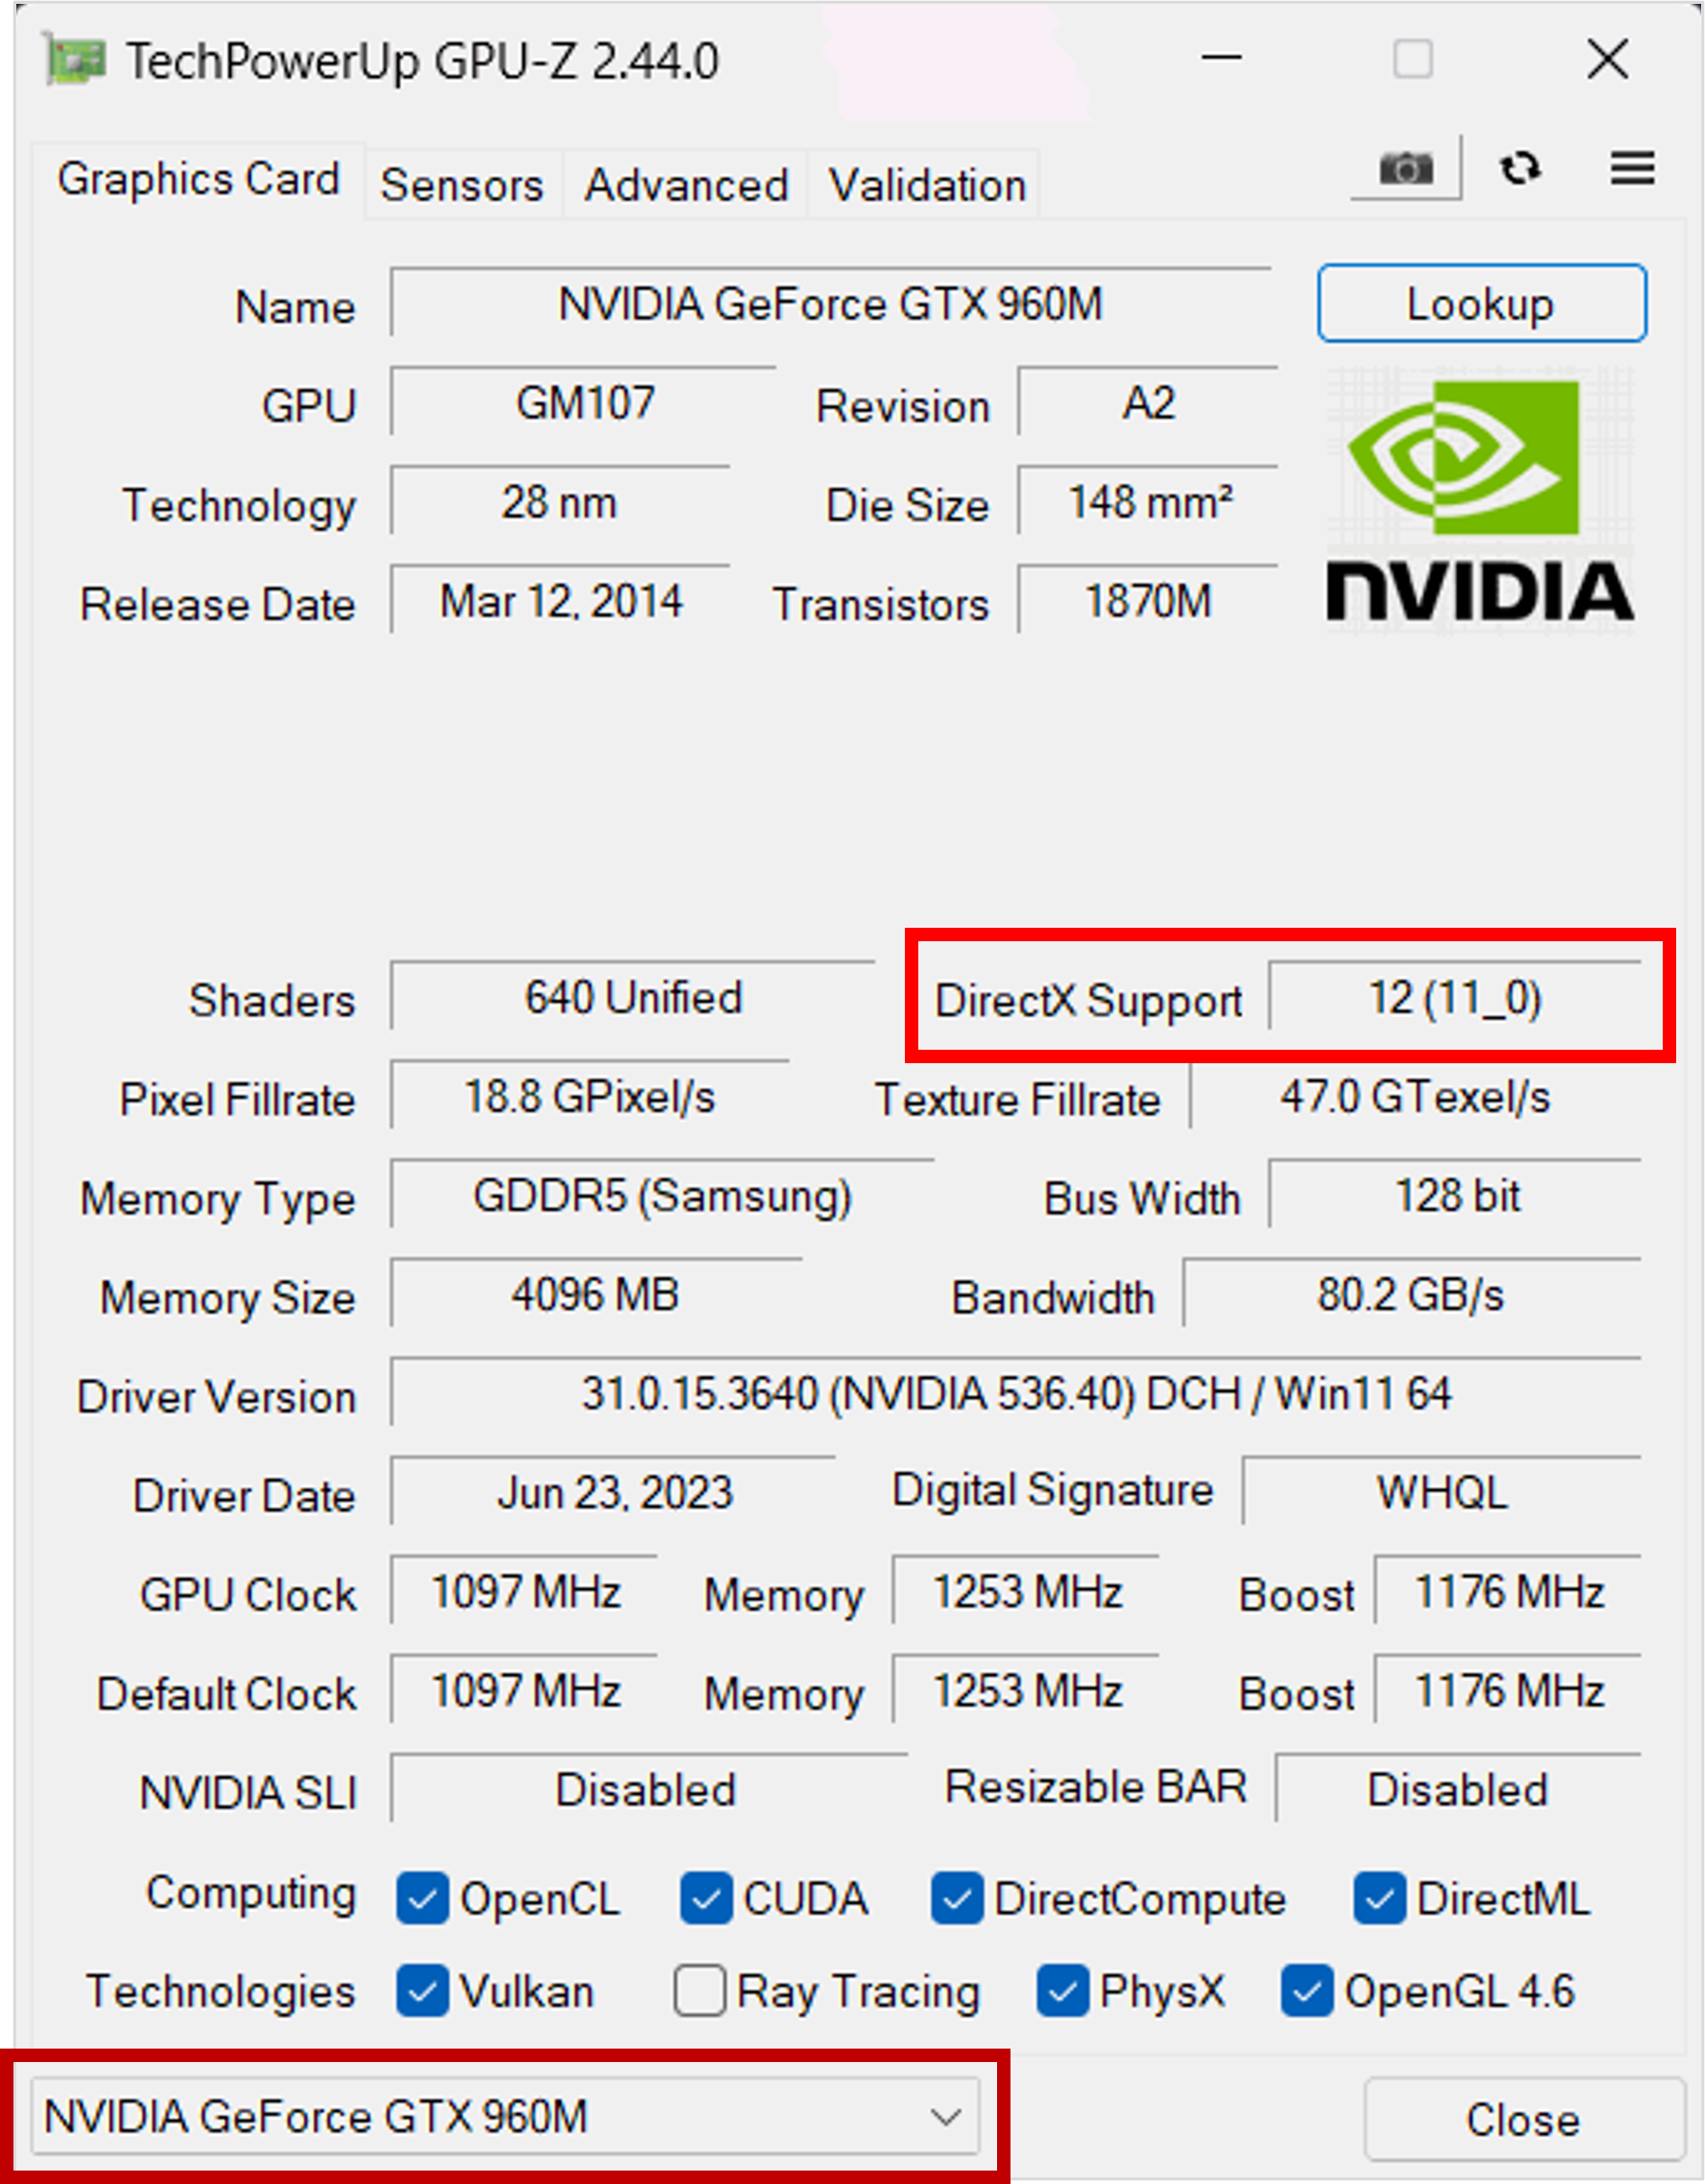
\includegraphics[scale=0.50]{Images/3/3.Intro.0.1}
                    \caption*{\Large محیط برنامه ی \lr{GPU-Z} \textbf{\vspace{12pt}}}
                \end{figure}
            \end{theo}
        }
    \end{enumerate}
}

\begin{theo}{thm:pythagoras}
    \Large
    تمامی کد های کتاب با کانفیگ های زیر تست شده اند:
    \lr{
        \begin{enumerate}
            \item {Windows 11 Pro 22H2 Build 22621.1992}
            \item {NVIDIA GeForce GTX 960m}
            \item {Visual Studio 2022 (64-bit) Version 17.1.2}
        \end{enumerate}
    }
\end{theo}

%-----------------------------------------------------------------------------------------------------------%

\title{
    \huge
    \hspace{-40pt}
    \textbf{استفاده از اسناد \lr{SDK DIRECTX} و نمونه های \lr{SDK}}
}  \rullFillWithLine[0.5em]{1pt}
\textbf{\vspace{7pt}}

{
    \Large
    \begin{spacing}{1.5}
        \lr{Direct3D} یک \lr{API} بزرگ است و ما نمی‌توانیم تمام جزئیات آن را در این یک کتاب پوشش دهیم.
        بنابراین، برای به دست آوردن اطلاعات بیشتر، ضروری است نحوه استفاده از اسناد \lr{DirectX SDK} را یاد بگیرید.
        به روزترین اسناد در \lr{\href{https://learn.microsoft.com/en-us/windows/win32/direct3d12/directx-12-programming-guide}{MSDN}} در دسترس خواهند بود.

        \begin{figure}[H]
            \centering
            \setlength{\belowcaptionskip}{-10pt}
            
\includegraphics[scale=0.15]{Images/3/3.Intro.0.2}
            \caption*{\normalsize \url{https://learn.microsoft.com/en-us/windows/win32/direct3d12/directx-12-programming-guide}}
            \label{fig:learn.microsoft.com}
        \end{figure}

        شکل \ref{fig:3.Intro.1.1} تصویری از مستندات آنلاین را نشان می‌دهد.
        اسناد \lr{DirectX} تقریباً همه‌ی بخش‌های \lr{DirectX API} را پوشش می‌دهد.
        بنابراین این اسناد می‌تواند یک مرجع بسیار مفید باشد، اما از آنجایی که مستندات آنچنان وارد جزئیات نمی‌شوند، می‌توان گفت که این اسناد بهترین ابزار یادگیری نیستند. با این حال، با هر نسخه جدید \lr{DirectX} که منتشر شود، اسناد نیز بهتر و بهتر می‌شود.

        \begin{figure}[H]
            \centering
            \setlength{\belowcaptionskip}{-10pt}
            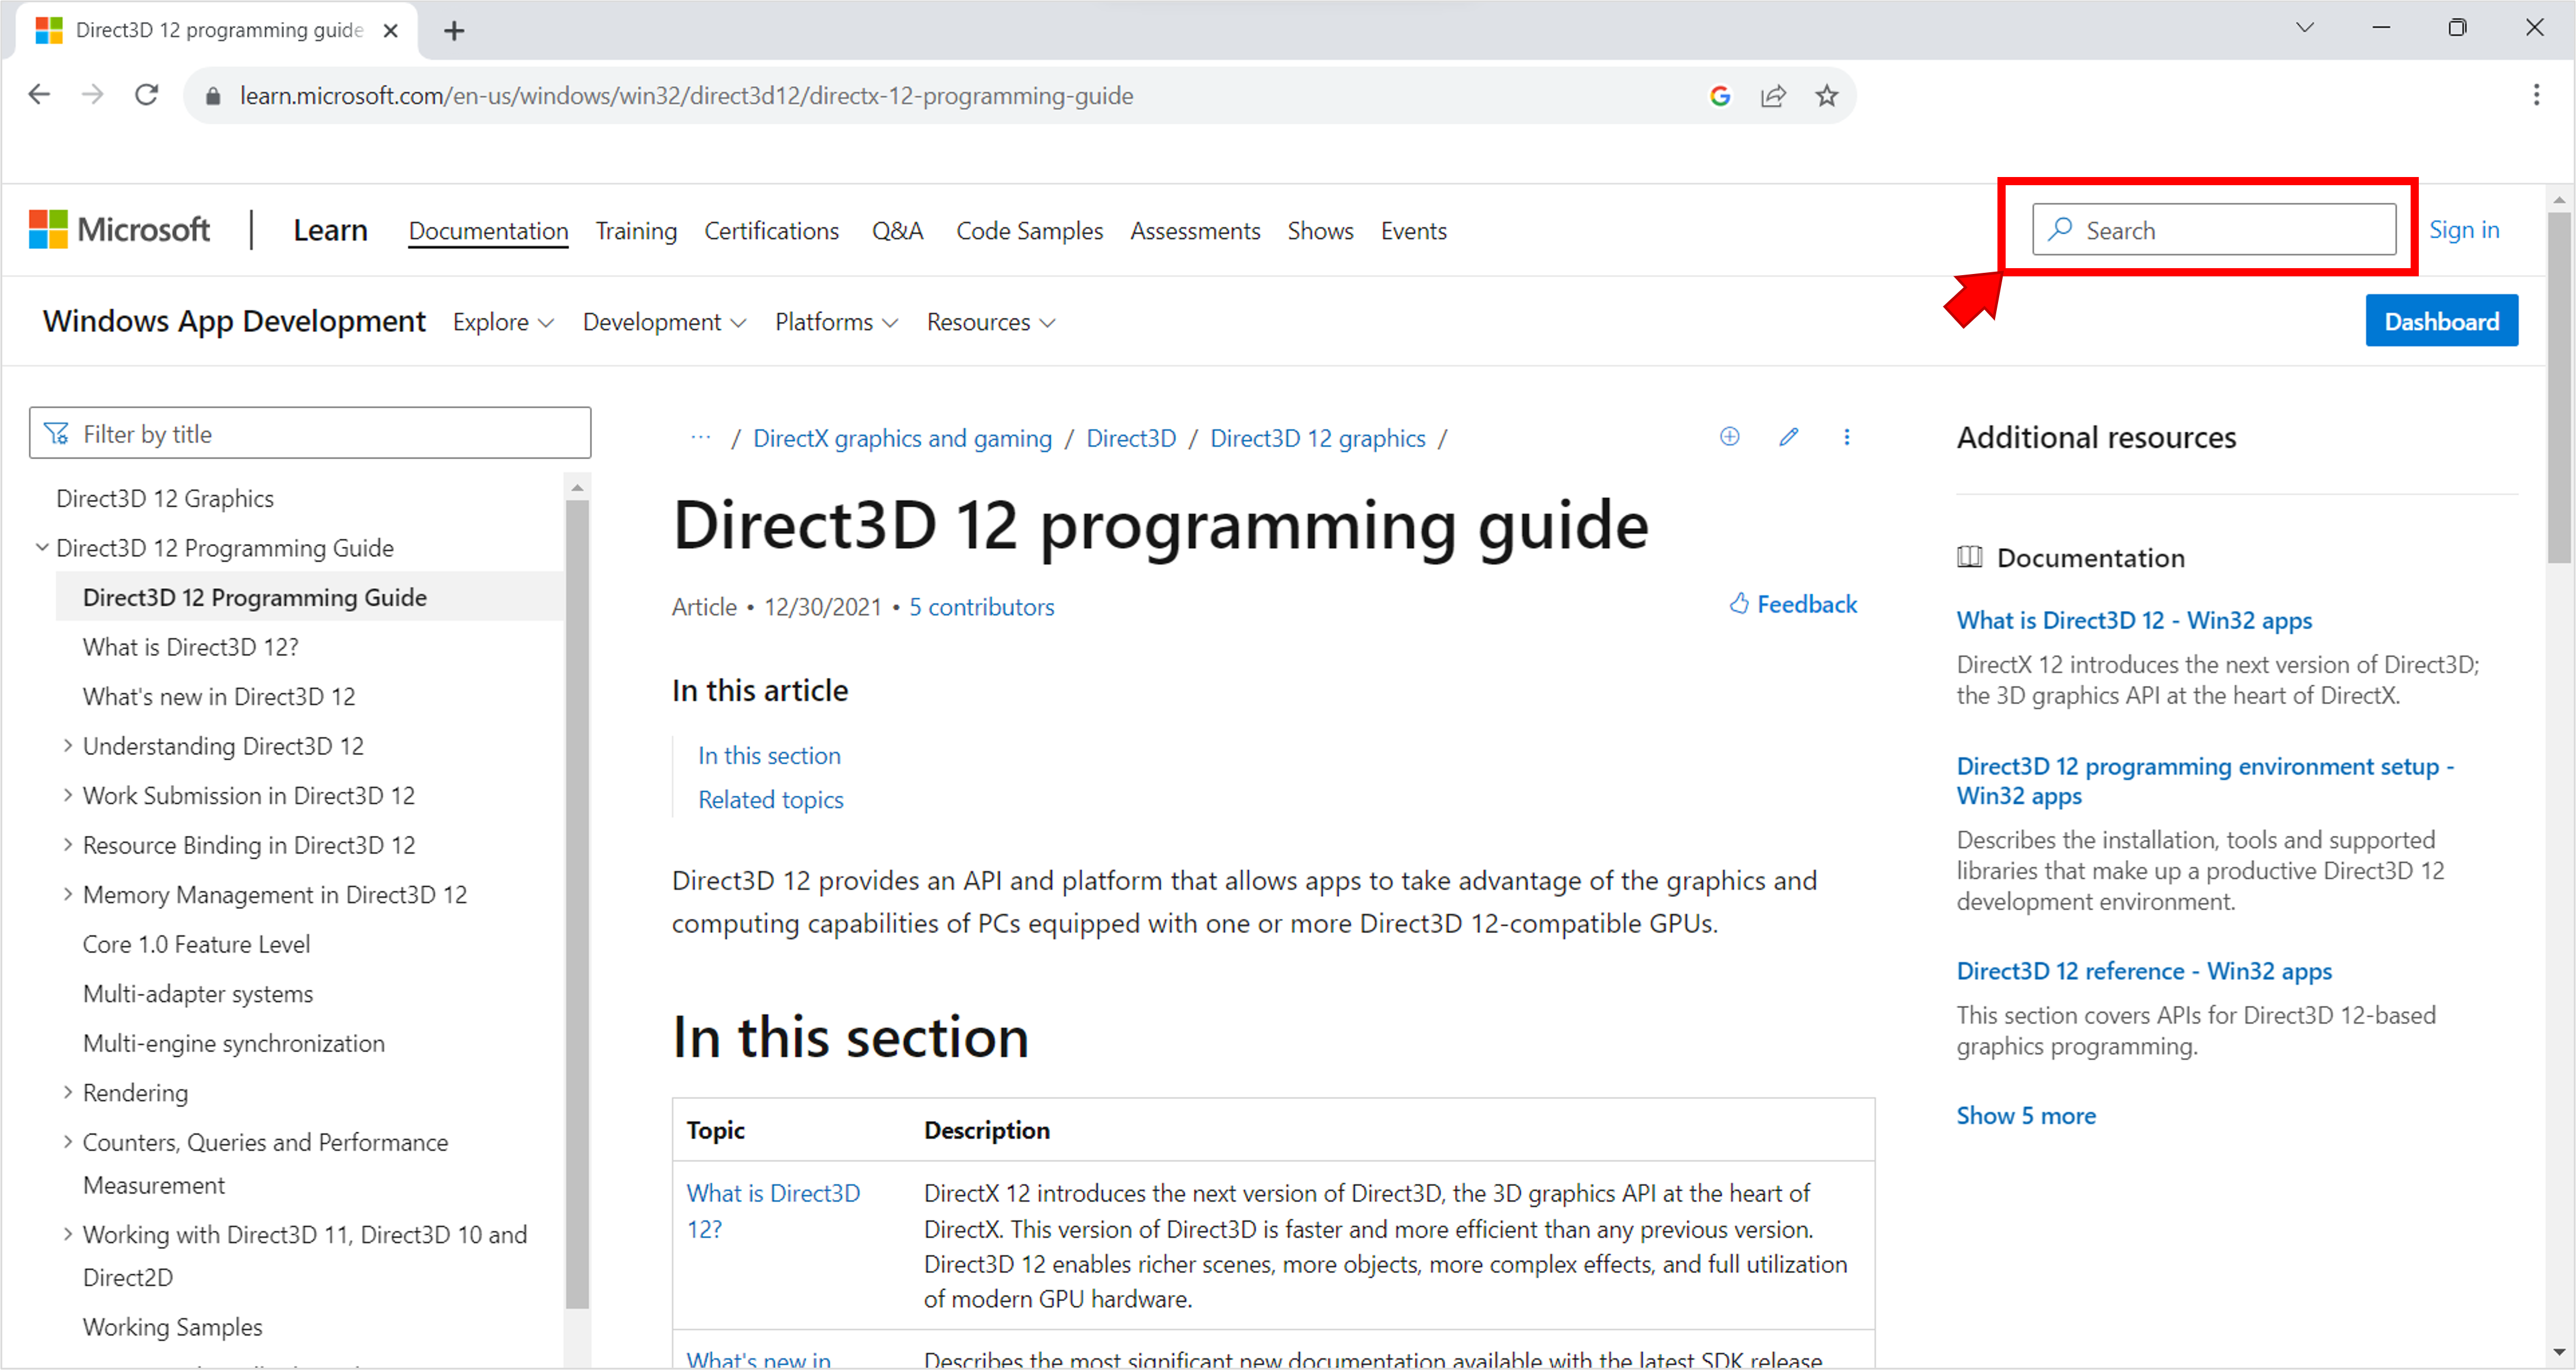
\includegraphics[width=\textwidth]{Images/3/3.Intro.1.1}
            \caption{راهنمای برنامه نویسی \lr{Direct3D} در مستندات \lr{DirectX}}
            \label{fig:3.Intro.1.1}
        \end{figure}

        همانطور که گفته شد، اسناد به عنوان یک مرجع قابل استفاده هستند.
        فرض کنید با یک نوع یا تابع مرتبط با \lr{DirectX} مواجه شده‌اید که اطلاعات بیشتری در مورد آن می‌خواهید، به عنوان مثال تابع \lr{\grayBox{ID3D12Device::CreateCommittedResource}}.
        شما می‌توانید به سادگی در مستندات جستجو کنید و توضیحاتی از نوع آن شی یا در این مثال، توضیحاتی در مورد تابع دریافت کنید. شکل \ref{fig:3.Intro.1.2} را ببینید.

        \begin{figure}[H]
            \centering
            \setlength{\belowcaptionskip}{-10pt}
            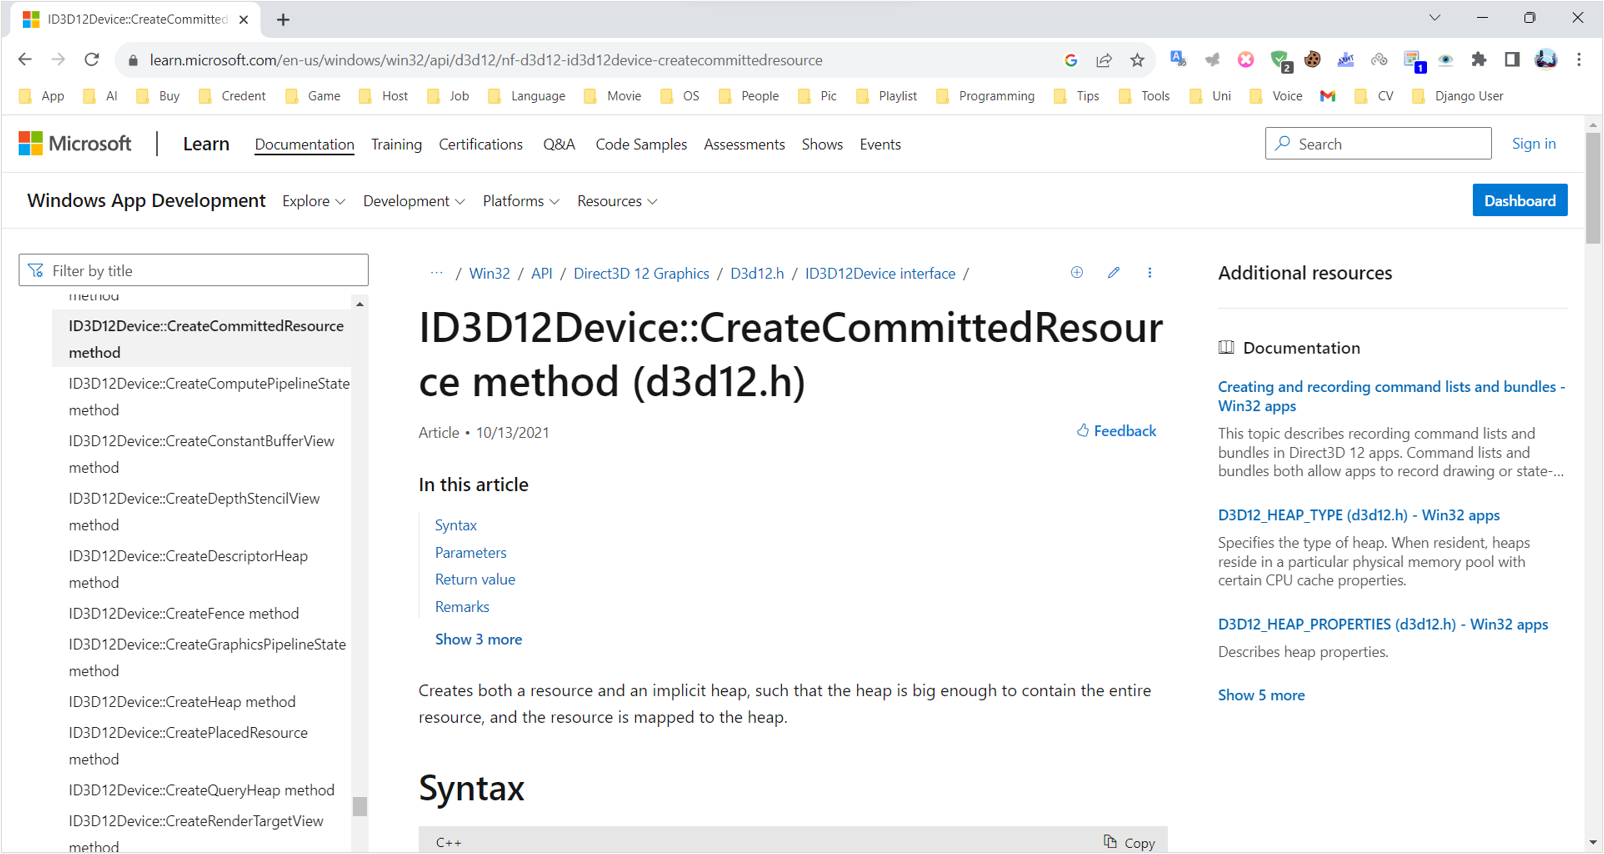
\includegraphics[width=\textwidth]{Images/3/3.Intro.1.2}
            \caption{دریافت مستندات یک تابع}
            \label{fig:3.Intro.1.2}
        \end{figure}

        \begin{theo}{thm:pythagoras}
            در این کتاب هر از گاهی برای جزئیات بیشتر شما را به مستندات راهنمایی می‌کنیم.
        \end{theo}
        همچنین برنامه های نمونه \lr{Direct3D 12} که به صورت آنلاین در دسترس هستند را میتوانید در لینک زیر مشاهده کنید:

        \begin{figure}[H]
            \centering
            \setlength{\belowcaptionskip}{-10pt}
            
\includegraphics[scale=0.15]{Images/3/3.Intro.1.3}
            \caption*{\Large \url{https://github.com/Microsoft/DirectX-Graphics-Samples}}
        \end{figure}

        میتوانید نمونه‌های \lr{Direct3D 12} را در وب‌سایت‌های \lr{NVIDIA}، \lr{AMD} و \lr{Intel} مشاهده کنید. همچنین در آینده نمونه‌های بیشتری نیز خواهند آمد.
    \end{spacing}
}
\textbf{\vspace{10pt}}

\title{
    \huge
    \hspace{-40pt}
    \textbf{شفاف سازی}
}  \rullFillWithLine[0.5em]{1pt}
\textbf{\vspace{7pt}}

{
    \Large
    \begin{spacing}{1.5}
        اگرچه ما تلاش می‌کنیم که کد‌های کارآمدی بنویسیم و همزمان از بهترین شیوه‌های برنامه‌نویسی \lr{Direct3D 12} استفاده کنیم، اما هدف اصلی هر برنامه‌ی نمونه، نشان دادن مفاهیم \lr{Direct3D} یا تکنیک‌های برنامه‌نویسی گرافیکی است.
        هدف ما نوشتن بهینه‌ترین کد نیست زیرا به احتمال زیاد، این کار‌ایده‌هایی را که تلاش می‌کردیم به تصویر بکشیم را مبهم می‌کرد.
        اگر از کد نمونه در پروژه‌های خود استفاده می‌کنید، این نکته را در نظر داشته باشید، زیرا باید برای کارایی بهتر دوباره روی آن کار کنید.
        علاوه بر این، به منظور تمرکز بر \lr{Direct3D API}، زیرساخت‌های حداقلی را در بالای \lr{Direct3D} ایجاد کرده‌ایم. به این معنی که ما مقادیر را هاردکد (\lr{hardcode}) کردیم و چیز‌هایی را در کد منبع تعریف کردیم که ممکن است مبتنی بر داده باشند.
        در یک برنامه بزرگ سه بعدی، احتمالاً یک موتور رندرینگ در بالای \lr{Direct3D} پیاده‌سازی خواهید کرد. با این حال، موضوع این کتاب \lr{Direct3D API} است، نه طراحی موتور‌های رندرینگ.
    \end{spacing}
}
\textbf{\vspace{10pt}}

\title{
    \huge
    \hspace{-40pt}
    \textbf{نمونه برنامه ها و مکمل های آنلاین}
}  \rullFillWithLine[0.5em]{1pt}
\textbf{\vspace{7pt}}

{
    \Large
    \begin{spacing}{1.5}
        وب‌سایت‌های این کتاب (\href{www.d3dcoder.net}{\lr{www.d3dcoder.net}} و \href{www.merclearning.com}{\lr{www.merclearning.com}}) نقش مهمی در استفاده حداکثری از این کتاب دارد. [\textbf{مترجم:} همه‌ی لینک‌ها و منابع در سایت من به صورت یکجا وجود دارند و نیازی نیست تمامی لینک‌های کتاب را ذخیره یا باز کنید.]
        در وب سایت شما کد منبع کامل و فایل‌های پروژه برای هر نمونه در این کتاب را خواهید یافت.
        در بسیاری از موارد، برنامه‌های \lr{DirectX} آنقدر بزرگ هستند که نمی‌توانند به طور کامل در یک کتاب متنی جاسازی شوند. بنابراین، ما فقط قطعات کد مربوطه را بر اساس‌ایده‌هایی که نشان داده می‌شوند نشان می‌دهیم.
        اکیداً توصیه می‌شود که خواننده کد آزمایشی مربوطه را مطالعه کند تا برنامه را به طور کامل ببیند (هدف ما این است که آزمایشی‌ها (\lr{demos}) را برای مطالعه آسان کوچک و متمرکز کنیم). به عنوان یک قاعده کلی، خواننده باید بتواند پس از خواندن فصل و گذراندن مدتی برای مطالعه کد نسخه‌ی آزمایشی، کد نسخه (ها)ی آزمایشی فصل را به تنهایی پیاده‌سازی کند.
        در واقع اینکه سعی کنید نمونه‌ها را خودتان با استفاده از کتاب و کد نمونه (به عنوان مرجع) پیاده‌سازی کنید، یک تمرین بسیار خوب است.
    \end{spacing}
}
\textbf{\vspace{10pt}}

%-----------------------------------------------------------------------------------------------------------%

\title{
    \huge
    \hspace{-40pt}
    \textbf{راه اندازی پروژه آزمایشی در \lr{Visual Studio 2022}}
}  \rullFillWithLine[0.5em]{1pt}
\textbf{\vspace{7pt}}

{
    \Large
    \begin{spacing}{1.5}
        آزمایشی‌های این کتاب را می‌توانید به سادگی با دوبار کلیک کردن روی فایل پروژه مربوطه \lr{(.vcxproj)} یا فایل \lr{solution (.sln)} باز کنید.
        این بخش نحوه‌ی باز کردن یا ایجاد و ساخت یک پروژه را از ابتدا با استفاده از چارچوب برنامه آزمایشی کتاب با استفاده از \lr{Visual Studio 2022} توضیح می‌دهد.
        به عنوان یک مثال کاربردی، نحوه بازآفرینی و \lr{build} کردن نسخه آزمایشی \enquote{\lr{Box}} از فصل 6 را نشان خواهیم داد.
    \end{spacing}
}

\textbf{\vspace{-30pt}}
\title{
    \LARGE
    \rullCenterTextWithLine{\textbf{کد منبع کتاب را دانلود کنید}}
}
\textbf{\vspace{-10pt}}

{
    \Large
    \begin{spacing}{1.5}
        ابتدا کد منبع کتاب را در پوشه‌ای در هارد دیسک خود دانلود کنید.
        فرض می‌کنیم این پوشه \grayBox{\lr{C:\symbol{92}d3d12book}} است.
        در پوشه کد منبع، فهرستی از پوشه‌ها از هر فصل را خواهید دید. هر پوشه شامل پروژه‌های کد برای فصل داده شده است.
        همچنین به پوشه‌ای به نام \grayBox{\lr{Common}} توجه کنید. این پوشه حاوی کد منبع به اشتراک گذاشته شده است که در تمام پروژه‌های آزمایشی استفاده مجدد می‌شود.
        اکنون، در پوشه کد منبع، یک پوشه جدید ایجاد کنید که می‌خواهید آزمایشی‌های خود را در آن ذخیره کنید.
        برای مثال، \grayBox{\lr{C:\symbol{92}d3d12book\symbol{92}MyDemos}}. این پوشه جایی است که می‌توانید پروژه‌های جدید را بر اساس چارچوب نمونه‌ی کتاب ایجاد کنید.
        این ساختار پوشه‌بندی ضروری نیست، اما ساختاری است که آزمایشی‌های کتاب از آن پیروی می‌کنند. اگر با تنظیم مسیر‌های اضافی راحت هستید، می‌توانید پروژه‌های آزمایشی خود را در هر مکانی قرار دهید و \lr{Visual Studio} را تنظیم کنید که کد منبع را در دایرکتوری \grayBox{\lr{Common}} پیدا کند.
    \end{spacing}
}

\begin{theo}{thm:pythagoras}
    \Large
    با آمدن \lr{Windows 8}، \lr{DirectX SDK} به عنوان بخشی از \lr{Windows SDK} گنجانده شد ، در صورتی که تا قبل از آن میتوانستید \lr{DirectX SDK} را به صورت جداگانه دانلود و نصب کنید ... .
    \textbf{برای اطلاعات بیشتر:} \href{https://learn.microsoft.com/en-us/windows/win32/directx-sdk--august-2009-}{\lr{Where is the DirectX SDK?}}
\end{theo}

\textbf{\vspace{-30pt}}
\title{
    \LARGE
    \rullCenterTextWithLine{\textbf{موارد مورد نیاز \lr{Visual Studio} را نصب کنید}}
}
\textbf{\vspace{-10pt}}

{
    \Large
    \begin{spacing}{1.5}
        در صورتی که \lr{Visual Studio} را نصب نکرده‌اید، ابتدا آن را با استفاده از راهنما‌های آنلاین نصب کنید. پس از نصب آن، ابتدا \lr{Visual Studio Installer} را باز کنید. از پنجره‌ی باز شده، \lr{Modify} یا \lr{Install} را کلیک کنید (شکل \ref{fig:3.Intro.2.1}).

        \begin{figure}[H]
            \centering
            \setlength{\belowcaptionskip}{-10pt}
            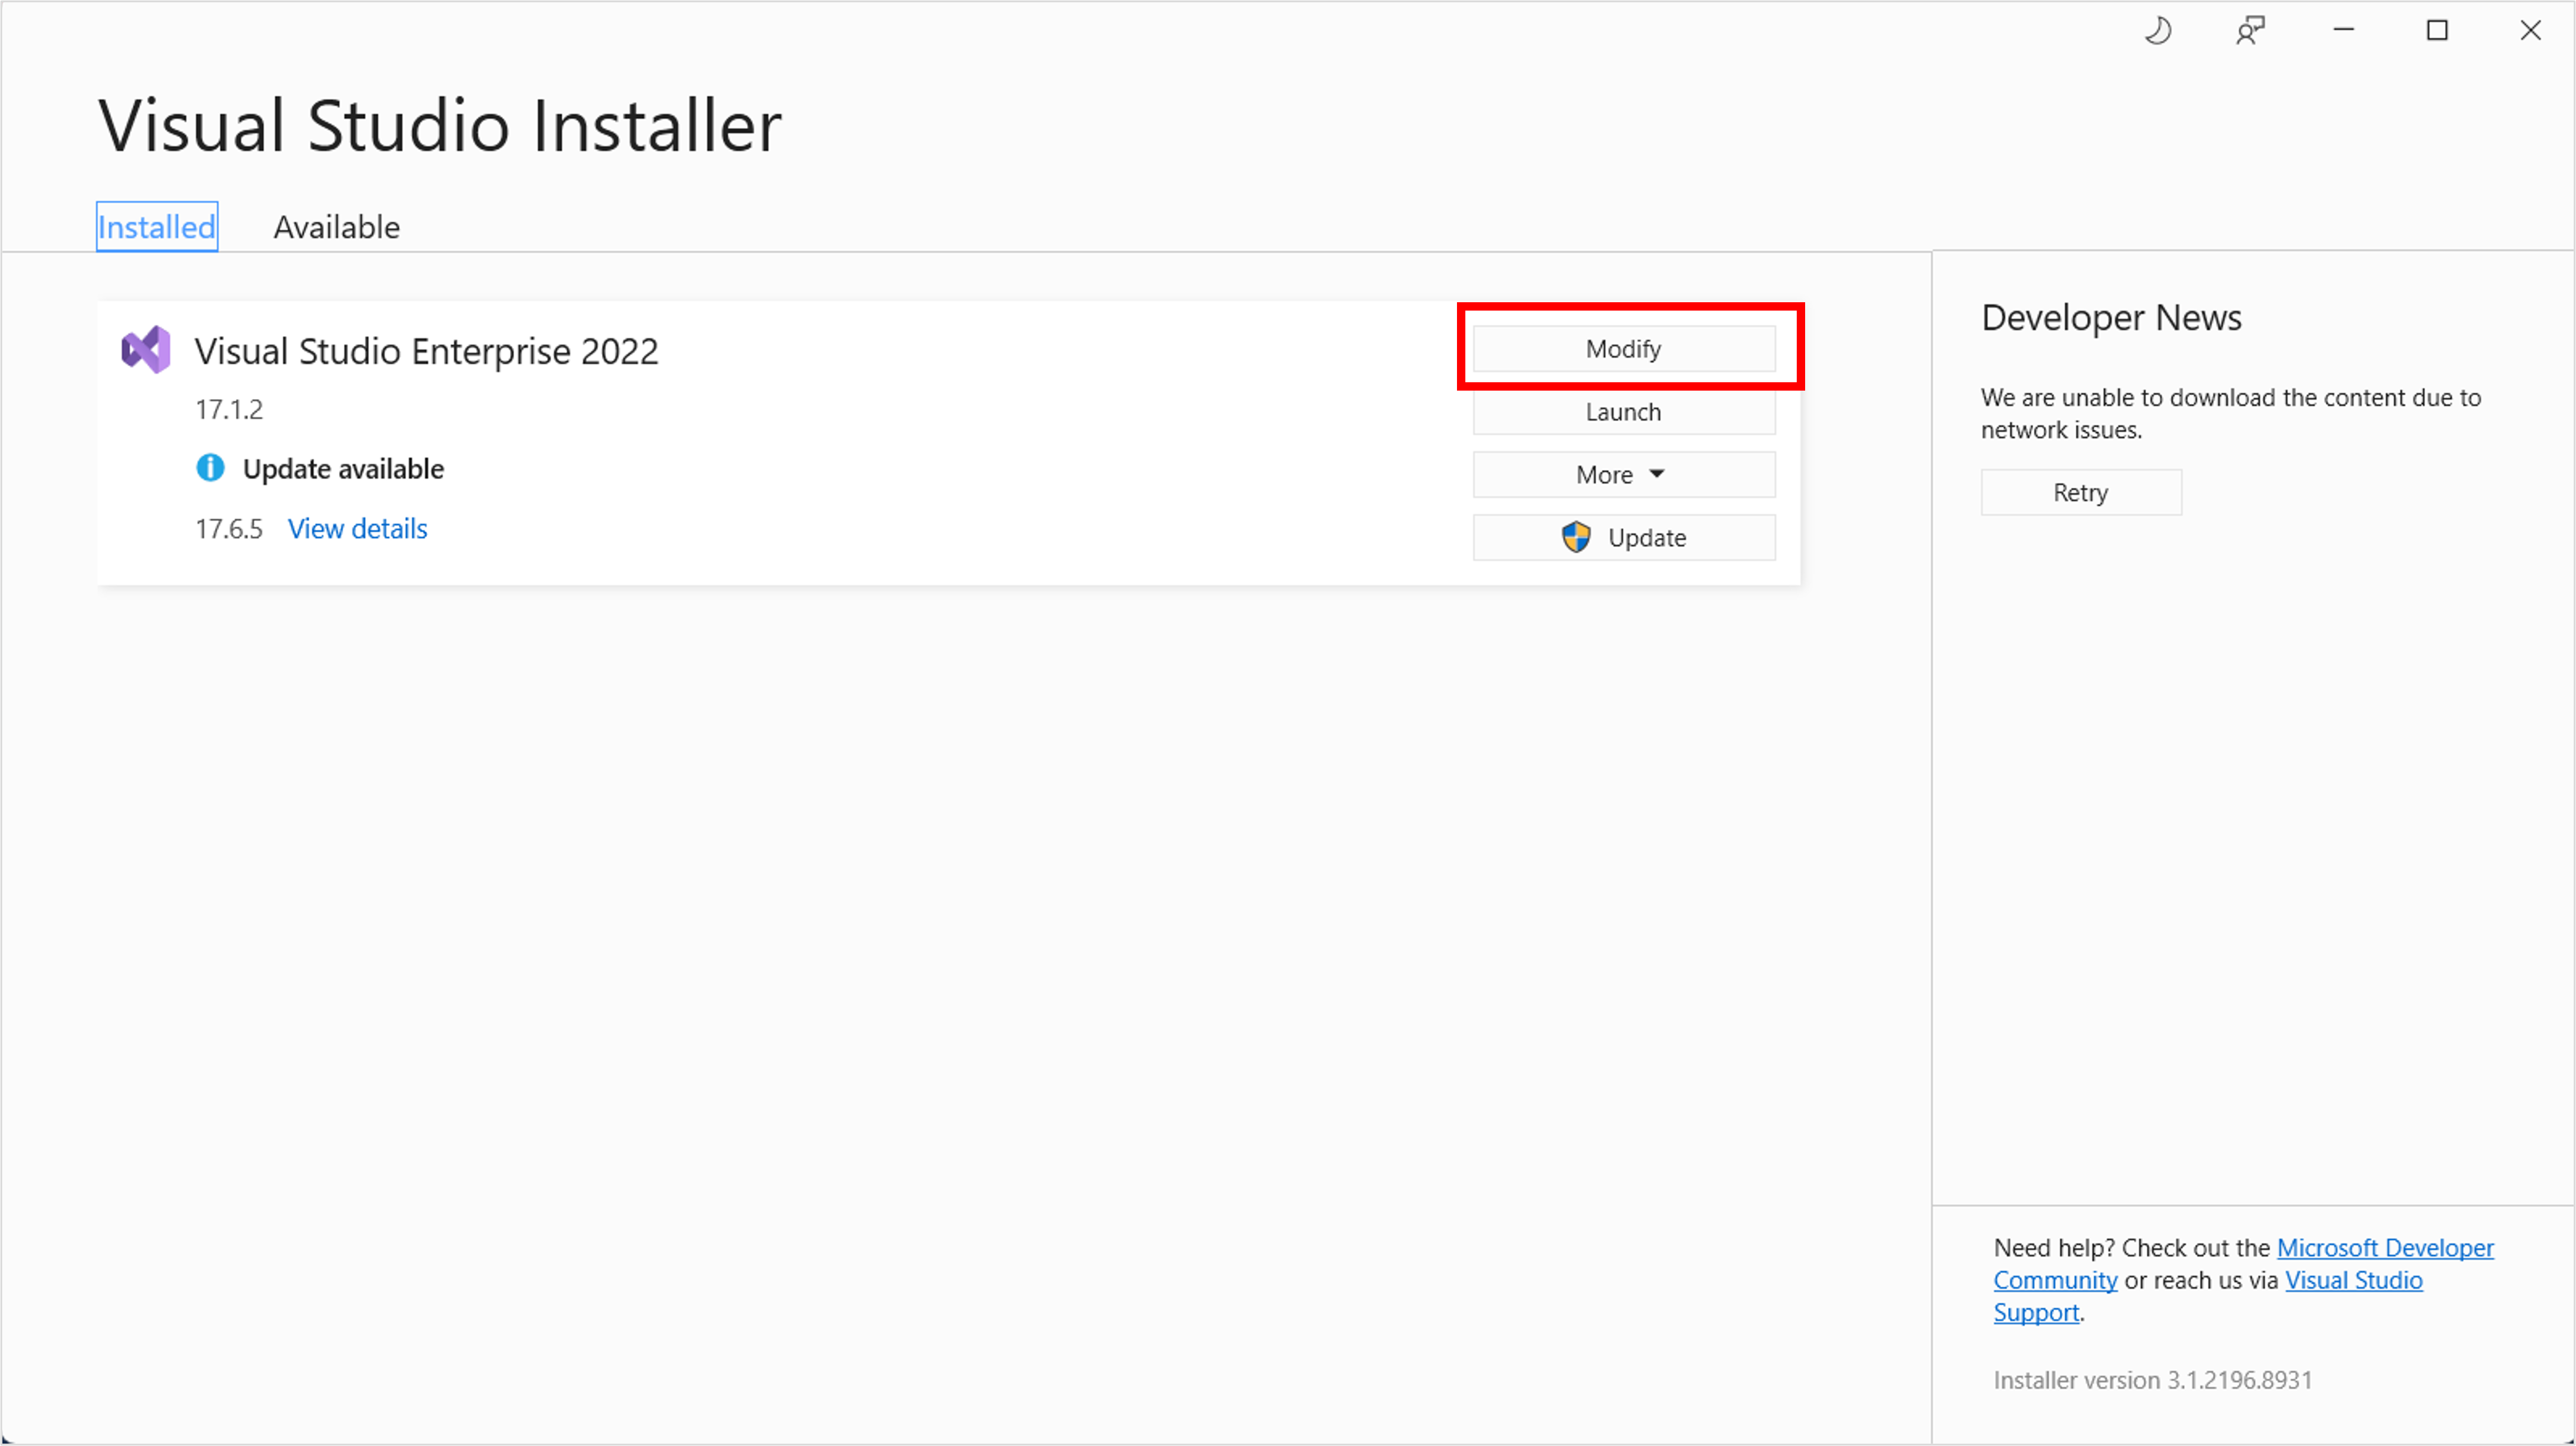
\includegraphics[width=\textwidth]{Images/3/3.Intro.2.1}
            \caption{محیط \lr{Visual Studio Installer}}
            \label{fig:3.Intro.2.1}
        \end{figure}

        در سمت چپ پنجره‌ی باز شده، از قسمت \lr{\grayBox{Desktop \& Mobile}}، تیک قسمت‌های \lr{Universal Windows Platform development} و \lr{Desktop development with C++} را در صورتی که انتخاب نشده‌اند، بزنید.
        از قسمت \lr{\grayBox{Gaming}} نیز تیک \lr{Game development with C++} را بزنید (شکل \ref{fig:3.Intro.2.2}).

        \begin{figure}[H]
            \centering
            \setlength{\belowcaptionskip}{-10pt}
            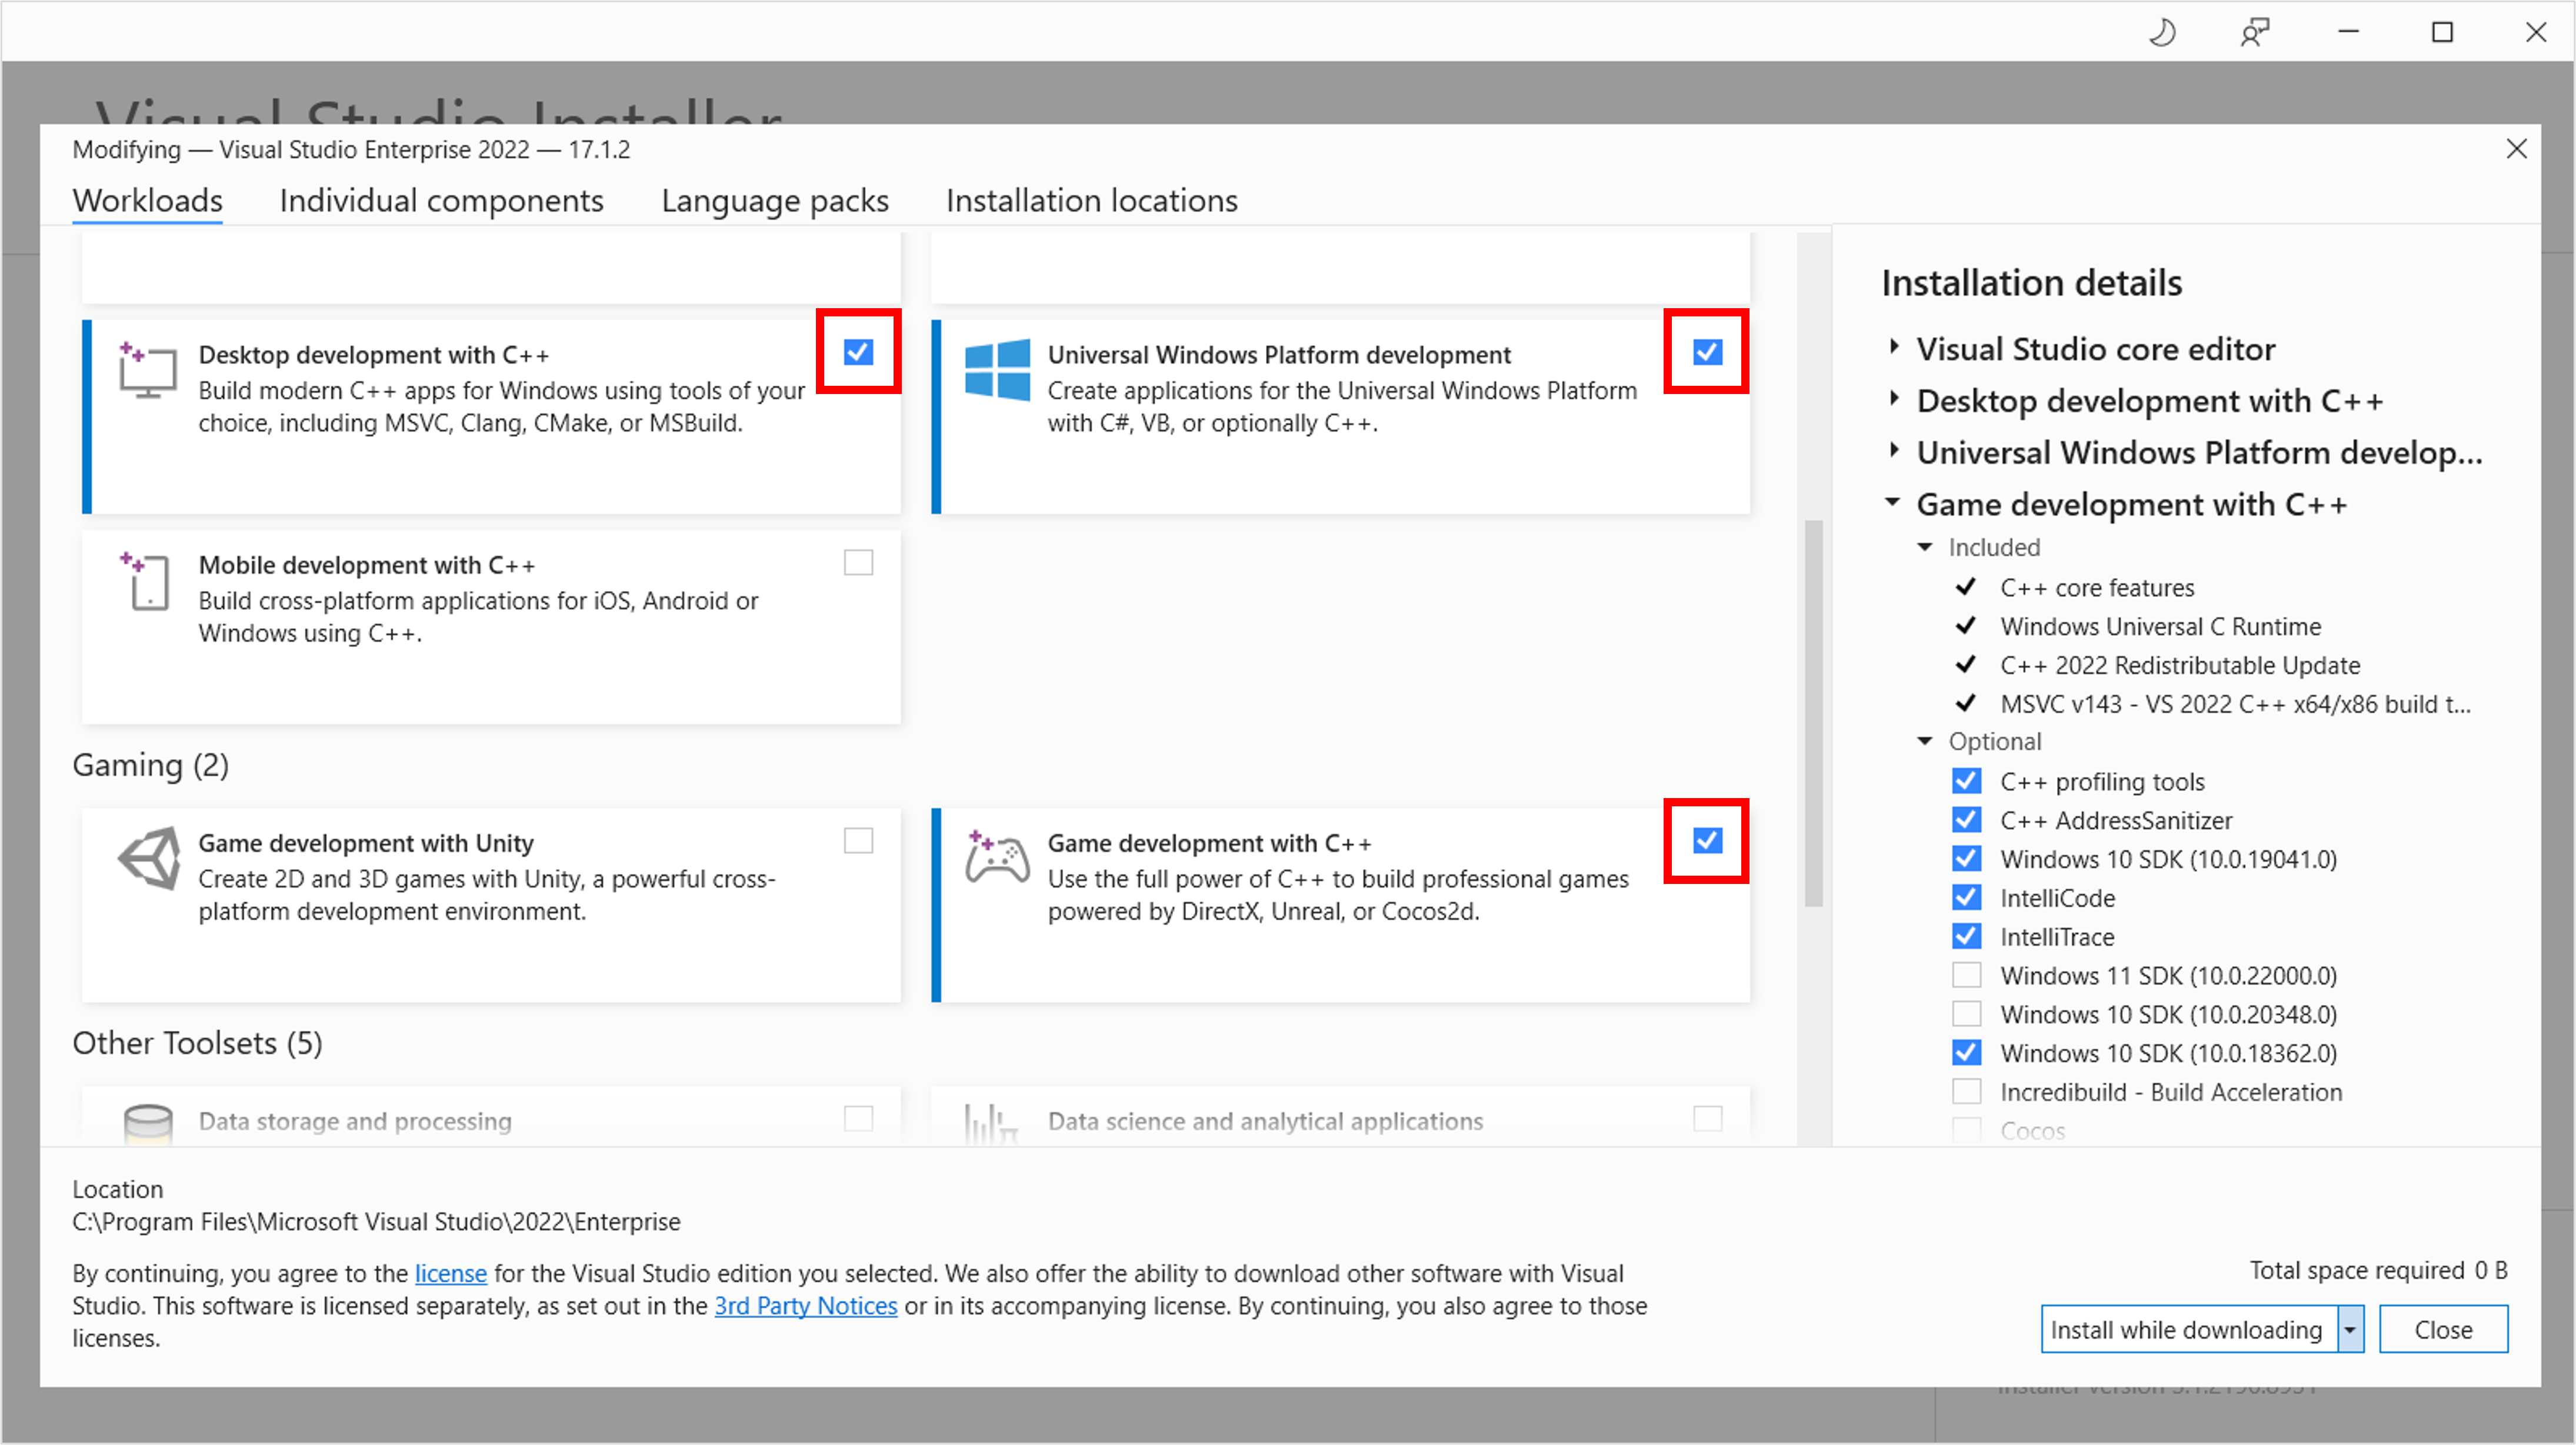
\includegraphics[width=\textwidth]{Images/3/3.Intro.2.2}
            \caption{مواردی که باید نصب شوند}
            \label{fig:3.Intro.2.2}
        \end{figure}

        بعد از انتخاب موارد بالا، باید موارد اضافه‌تری را نیز انتخاب کنید. این موارد شامل \lr{SDK}‌های ویندوز و ورژن‌های جدید \lr{C++} است.
        در سمت راست پنجره‌ی باز شده، می‌توانید این موارد را ببینید. برای اجرای بهتر، سعی کنید موارد را مانند عکس‌ها رعایت کنید. پس از آن در پایین پنجره روی گزینه‌ی \lr{Install} کلیک کنید تا موارد انتخاب شده نصب شوند.

        \begin{figure}[H]
            \centering
            \setlength{\belowcaptionskip}{-10pt}
            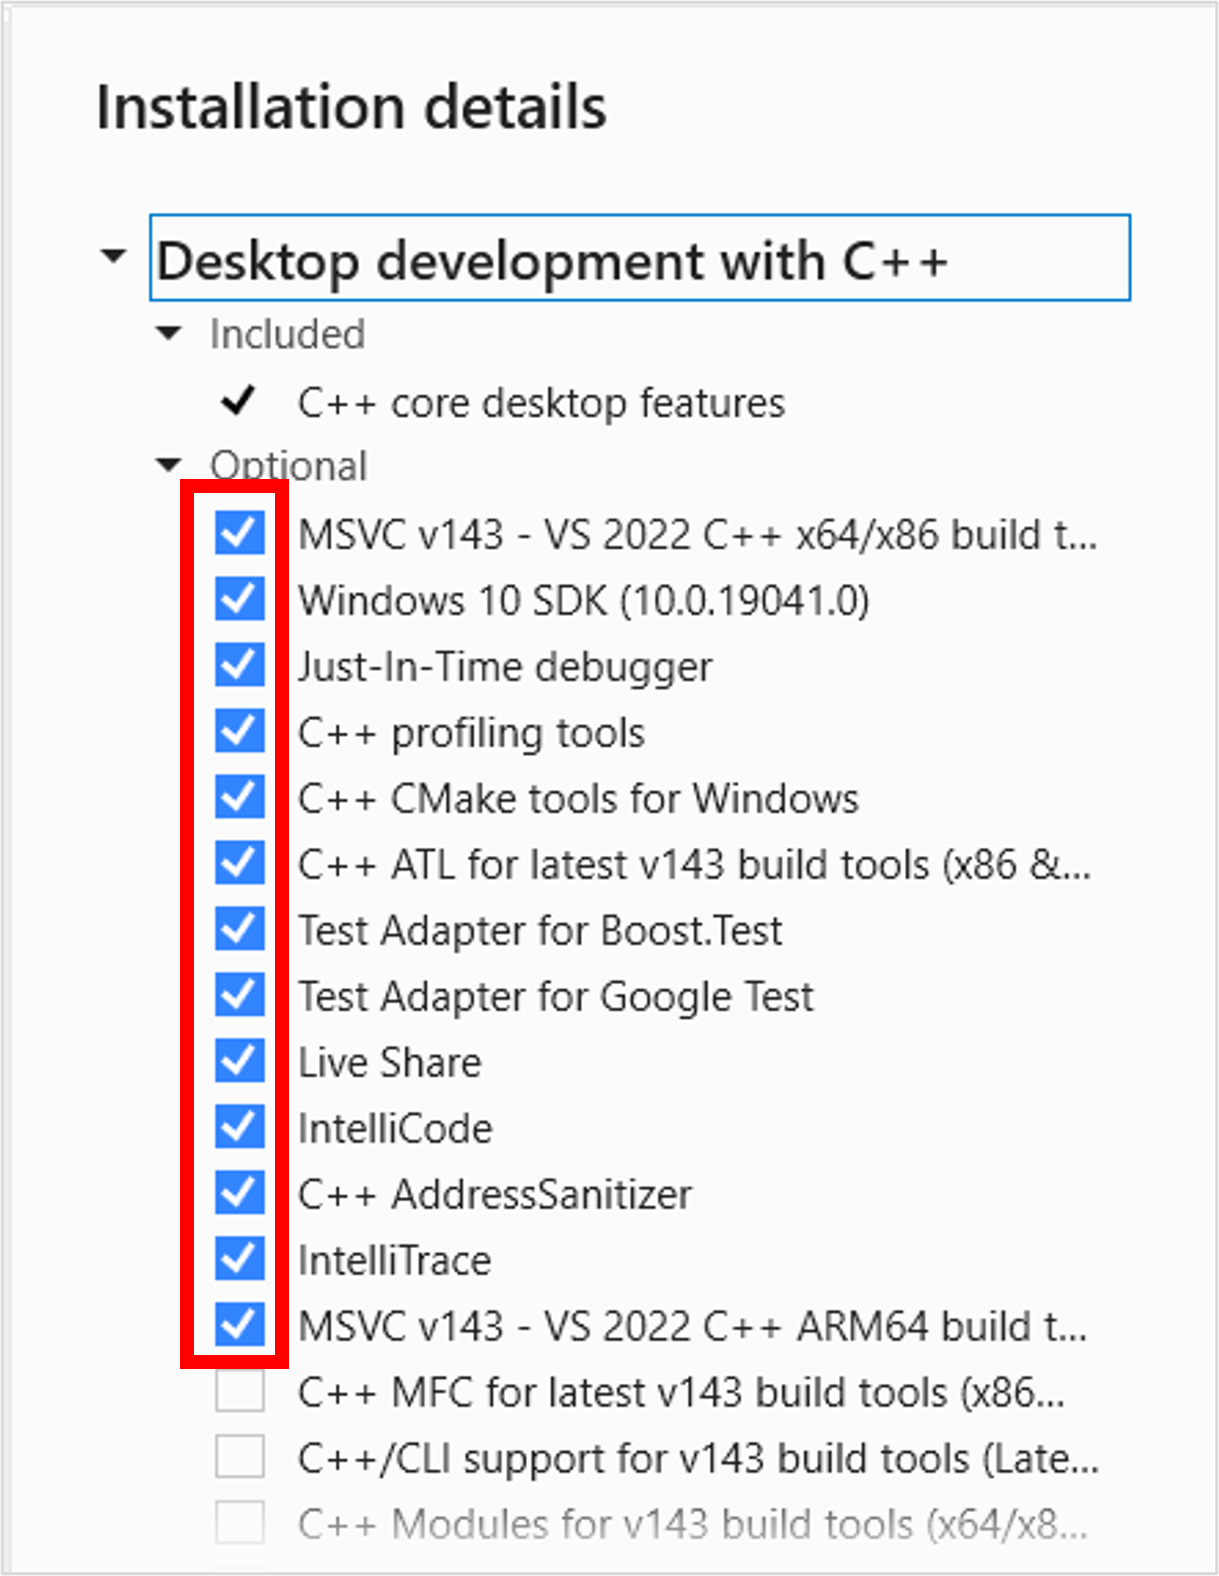
\includegraphics[scale=0.6]{Images/3/3.Intro.3.1} \hspace{5mm}
            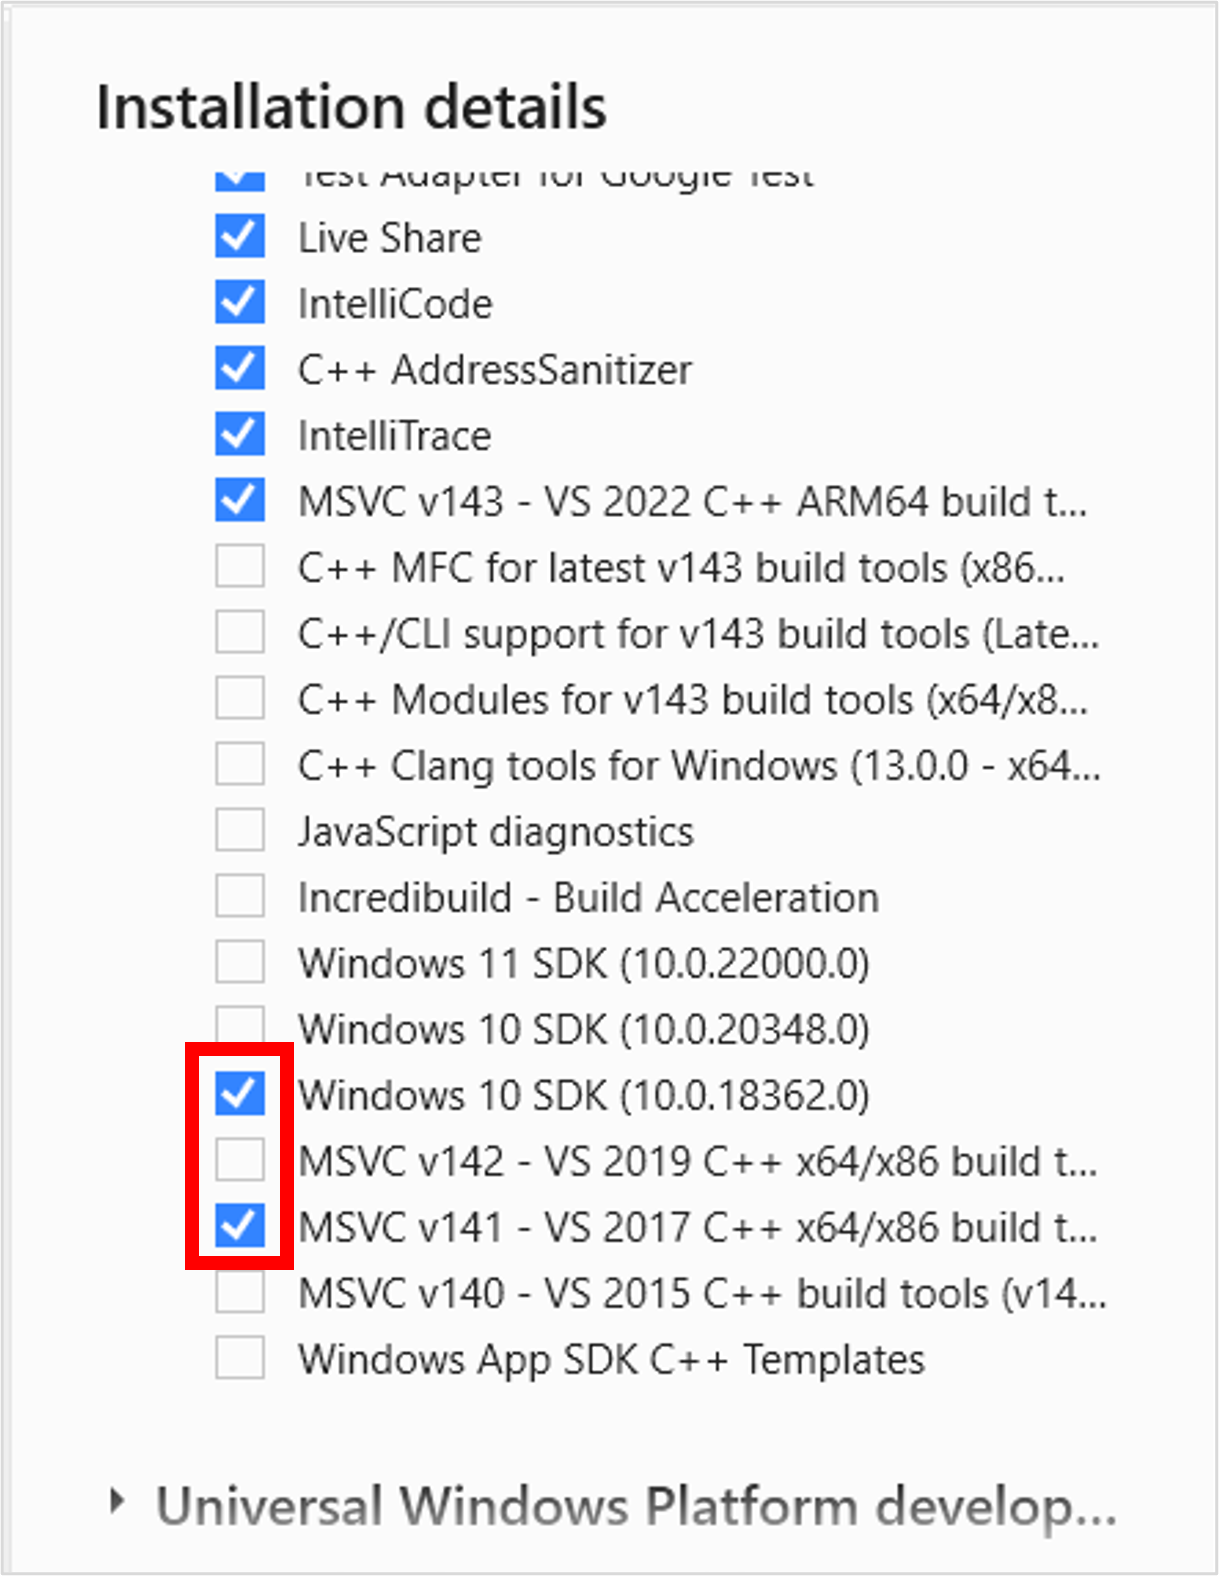
\includegraphics[scale=0.6]{Images/3/3.Intro.3.2}
            \caption*{مواردی که باید نصب شوند. (1)}
        \end{figure}

        \begin{figure}[H]
            \centering
            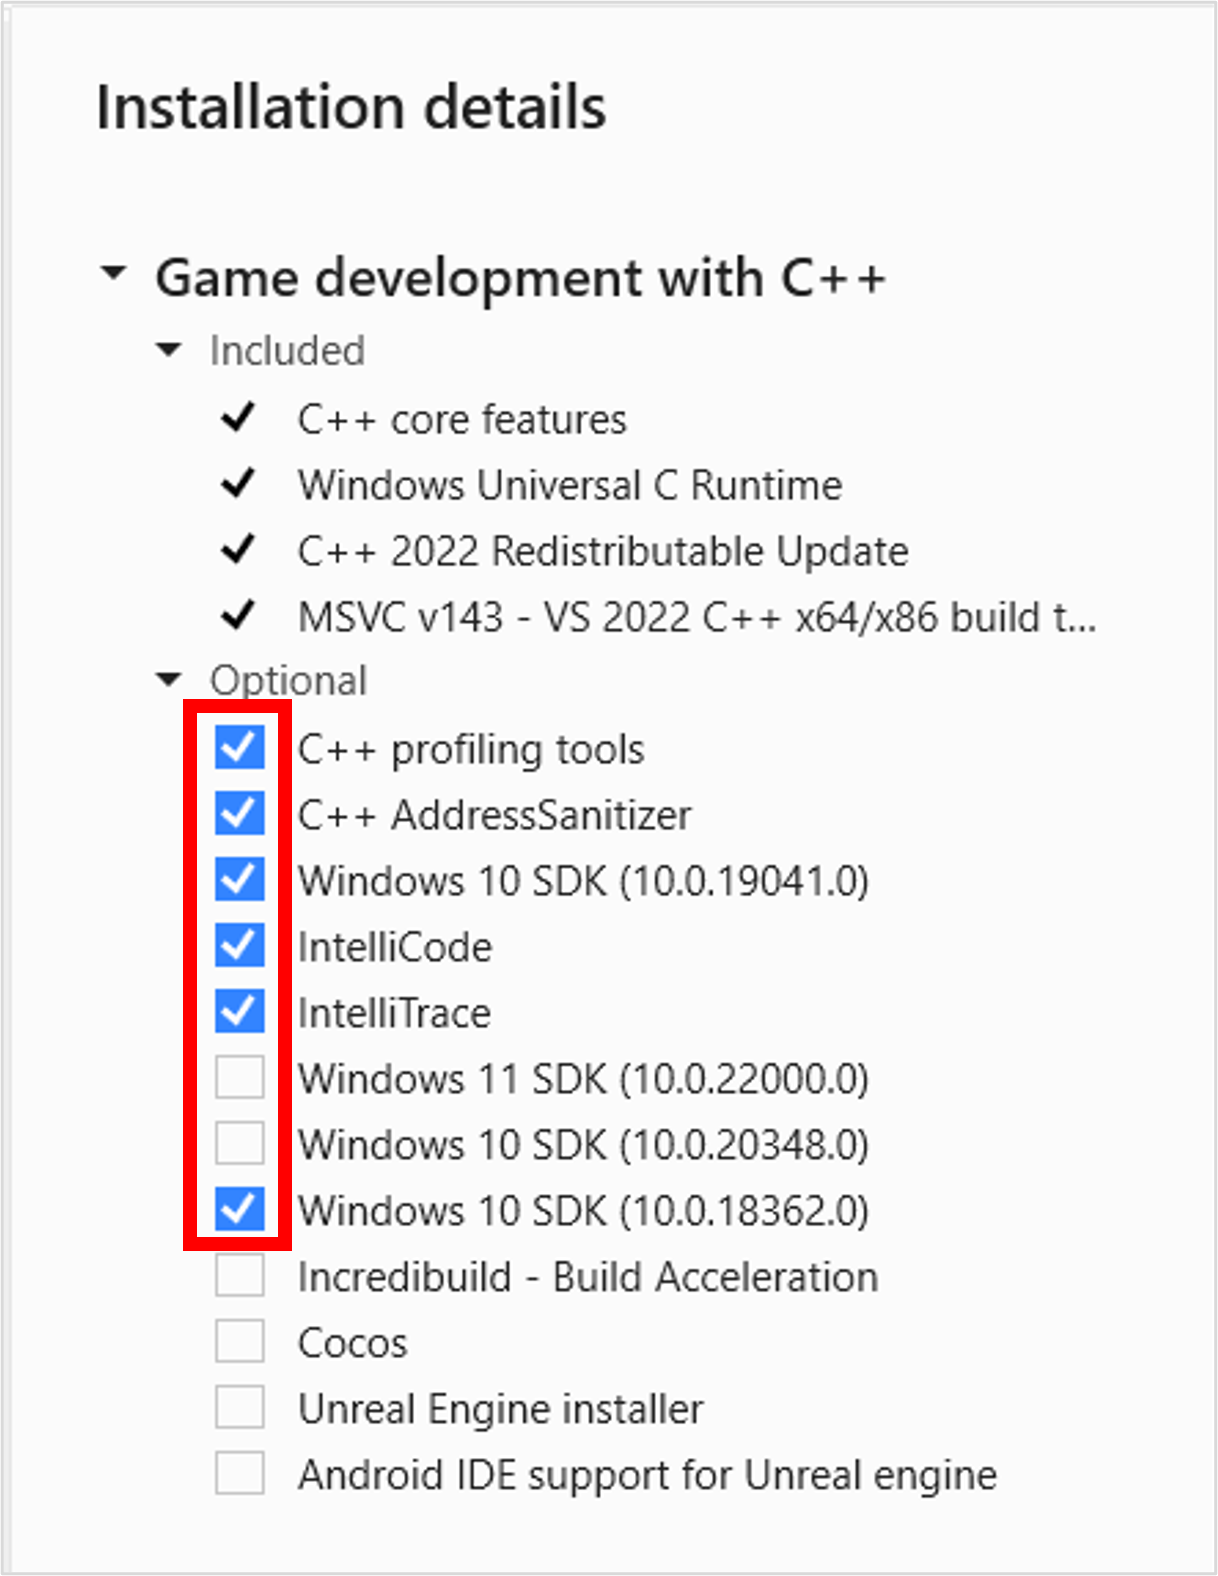
\includegraphics[scale=0.6]{Images/3/3.Intro.3.3} \hspace{5mm}
            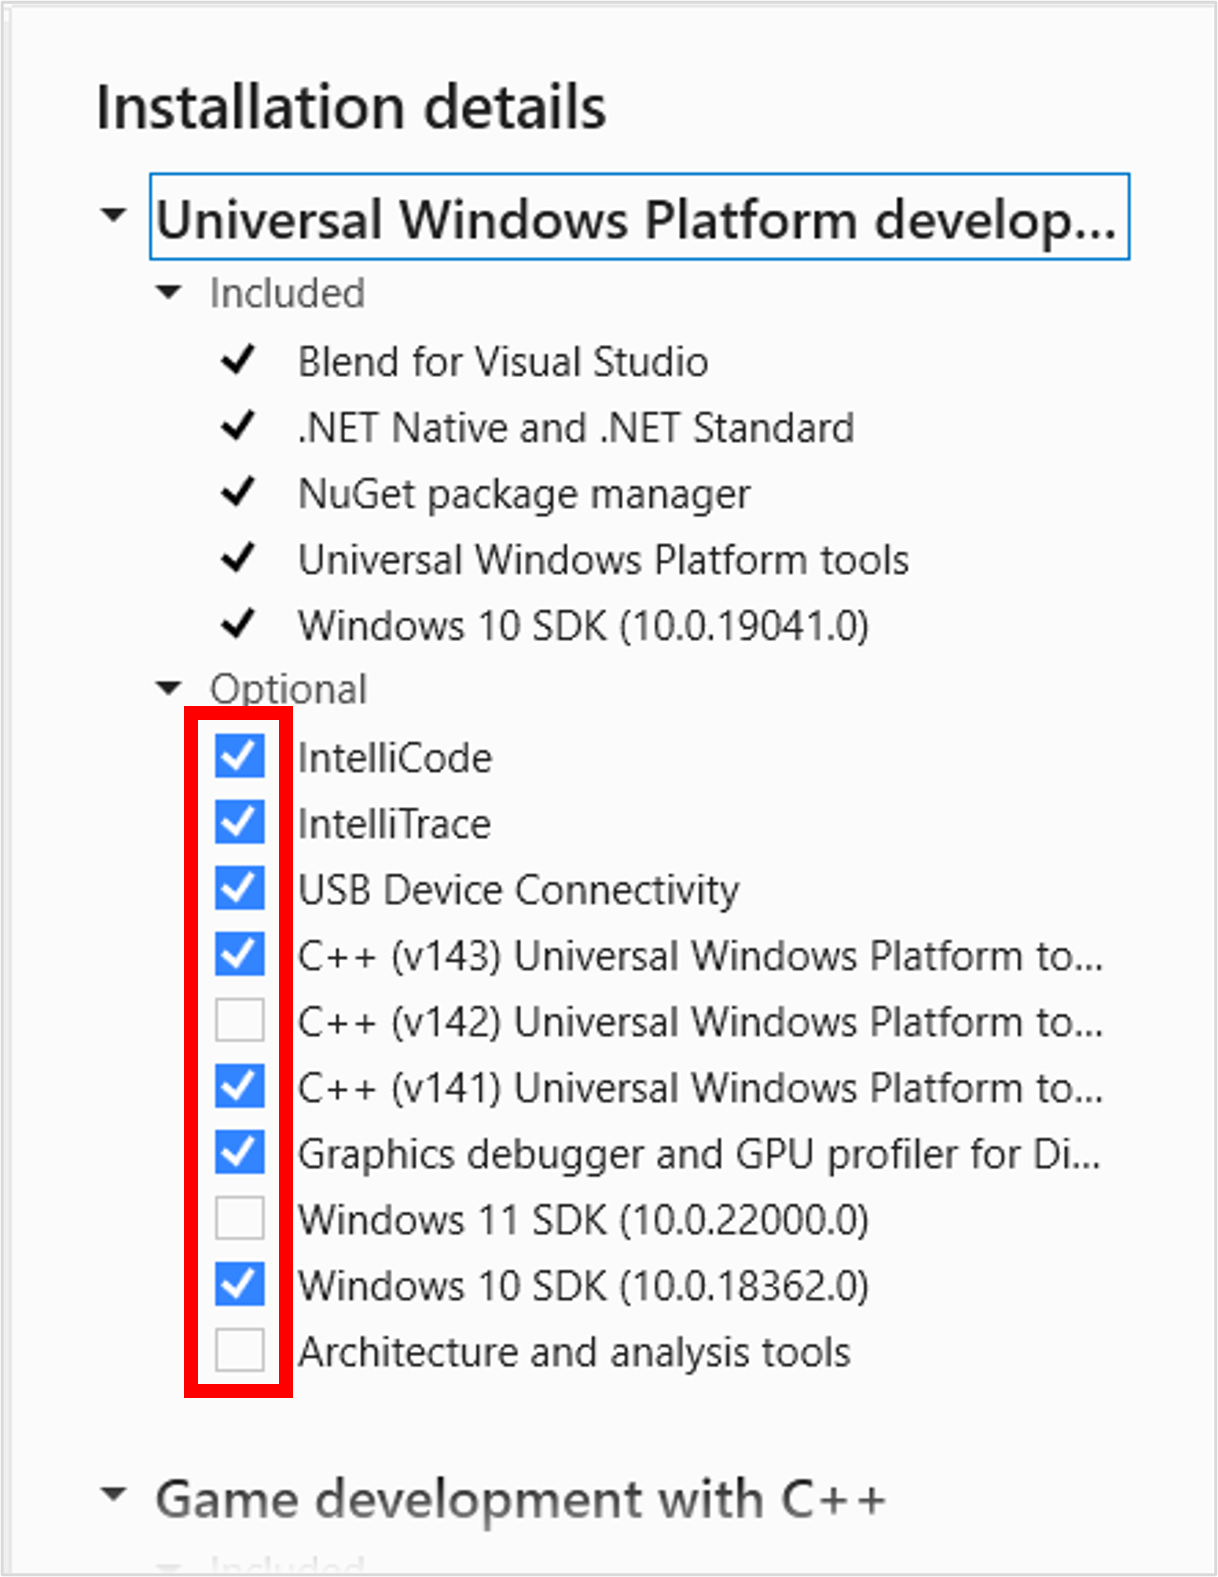
\includegraphics[scale=0.6]{Images/3/3.Intro.3.4}
            \caption*{مواردی که باید نصب شوند. (2)}
        \end{figure}
    \end{spacing}
}

\textbf{\vspace{-30pt}}
\title{
    \LARGE
    \rullCenterTextWithLine{\textbf{فعال کردن \lr{Graphic Tools}}}
}
\textbf{\vspace{-10pt}}

{
    \Large
    \begin{spacing}{1.5}
        برای اجرای درست برنامه‌های آزمایشی \lr{DirectX 12}، نیاز است که قابلیت \lr{Graphic Tools} در ویندوز شما فعال باشد.
        برای این کار می‌توانید به دو صورت عمل کنید:

        \textbf{روش اول)}
        ابتدا در منوی استارت، \lr{Optional features} را سرچ کرده و آن را باز کنید.
        اگر \lr{Graphic Tools} بر روی دستگاه نصب باشد، می‌توانید آن را در کادر زرد مشاهده کنید (شکل \ref{fig:3.Intro.4.1})

        \begin{figure}[H]
            \centering
            \setlength{\belowcaptionskip}{-10pt}
            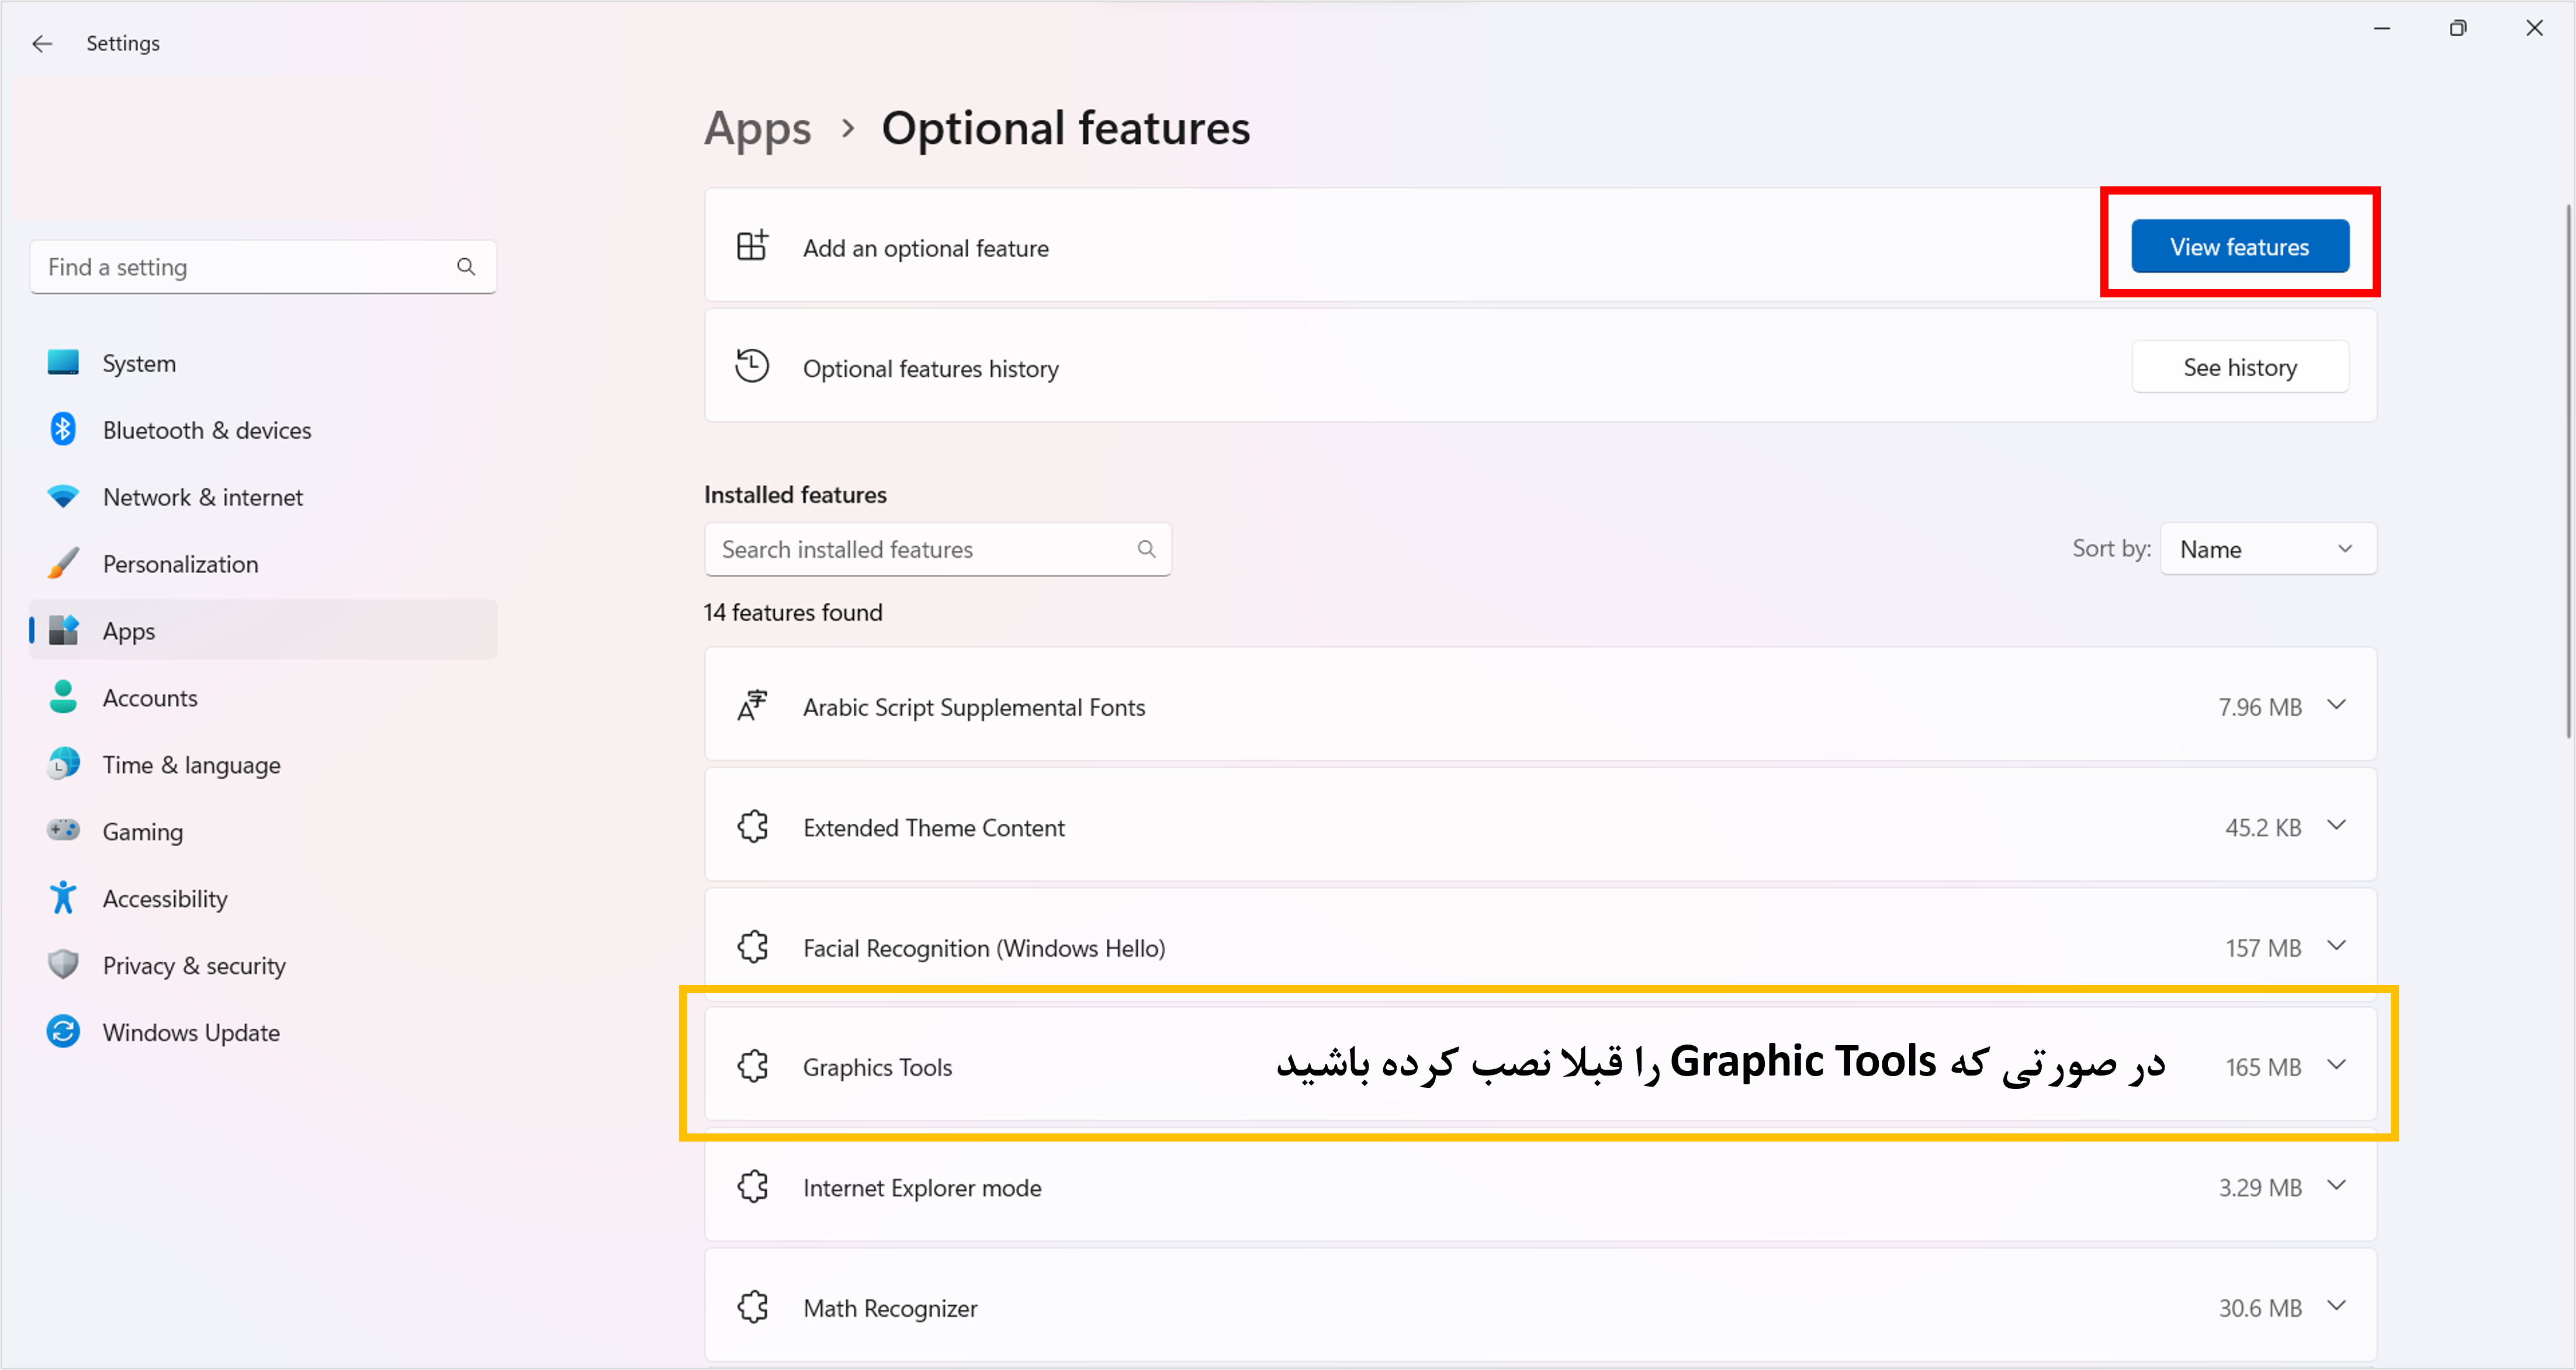
\includegraphics[width=\textwidth]{Images/3/3.Intro.4.1}
            \caption{محیط \lr{Optional features}}
            \label{fig:3.Intro.4.1}
        \end{figure}

        در صورتی که نصب نبود ، بر روی \lr{\grayBox{View features}} کلیک کرده و نام آن را سرچ کرده و نصب کنید (شکل \ref{fig:3.Intro.4.2}).

        \begin{figure}[H]
            \centering
            \setlength{\belowcaptionskip}{-10pt}
            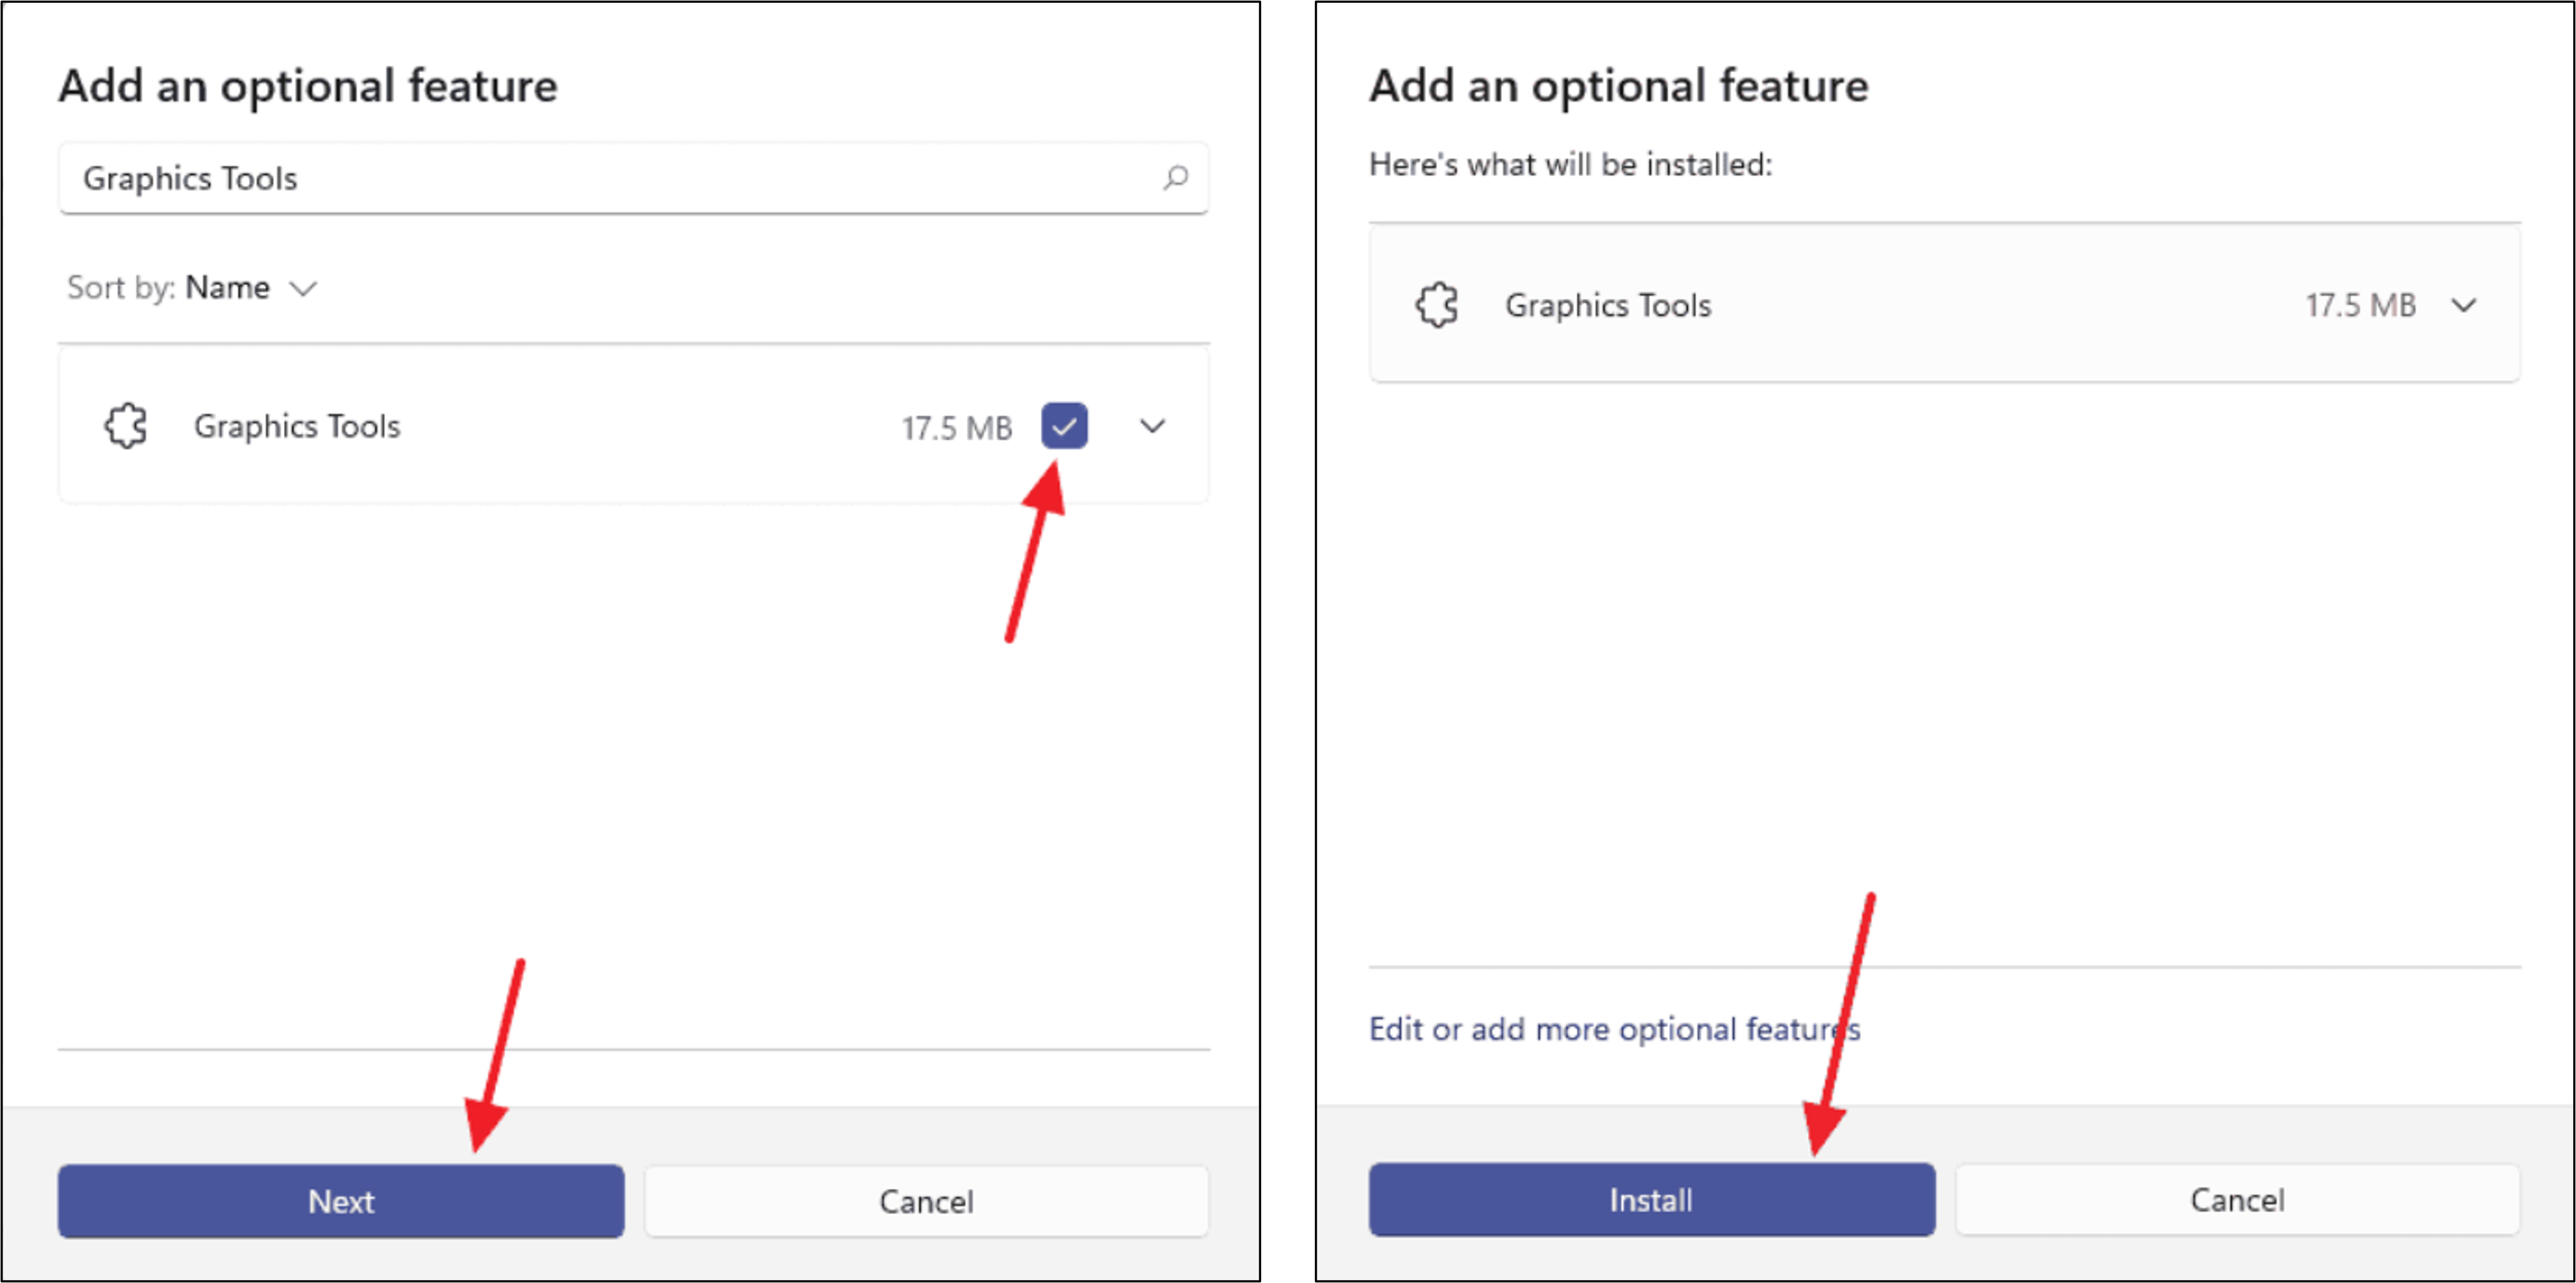
\includegraphics[width=\textwidth]{Images/3/3.Intro.4.2}
            \caption{نصب \lr{Graphic Tools}}
            \label{fig:3.Intro.4.2}
        \end{figure}

        \textbf{روش دوم)}
        اگر به هر دلیلی روش اول برای شما قابل انجام نبود، می‌توانید پنجره‌ی \lr{Command Prompt} (\lr{CMD}) را به صورت \lr{Run as administrator} باز کرده و با دستورات زیر آن را نصب کنید.
        در ابتدا دستور داخل \lr{CMD} عبارت زیر را وارد کنید:

        \begin{flushleft}
            \grayBox{\lr{Dism /Online /Get-Packages /Format:Table}}
        \end{flushleft}

        یا دستور زیر را وارد کنید:

        \begin{flushleft}
            \grayBox{\lr{Dism /Online /Get-Capabilities}}
        \end{flushleft}

        \begin{figure}[H]
            \centering
            \setlength{\belowcaptionskip}{-10pt}
            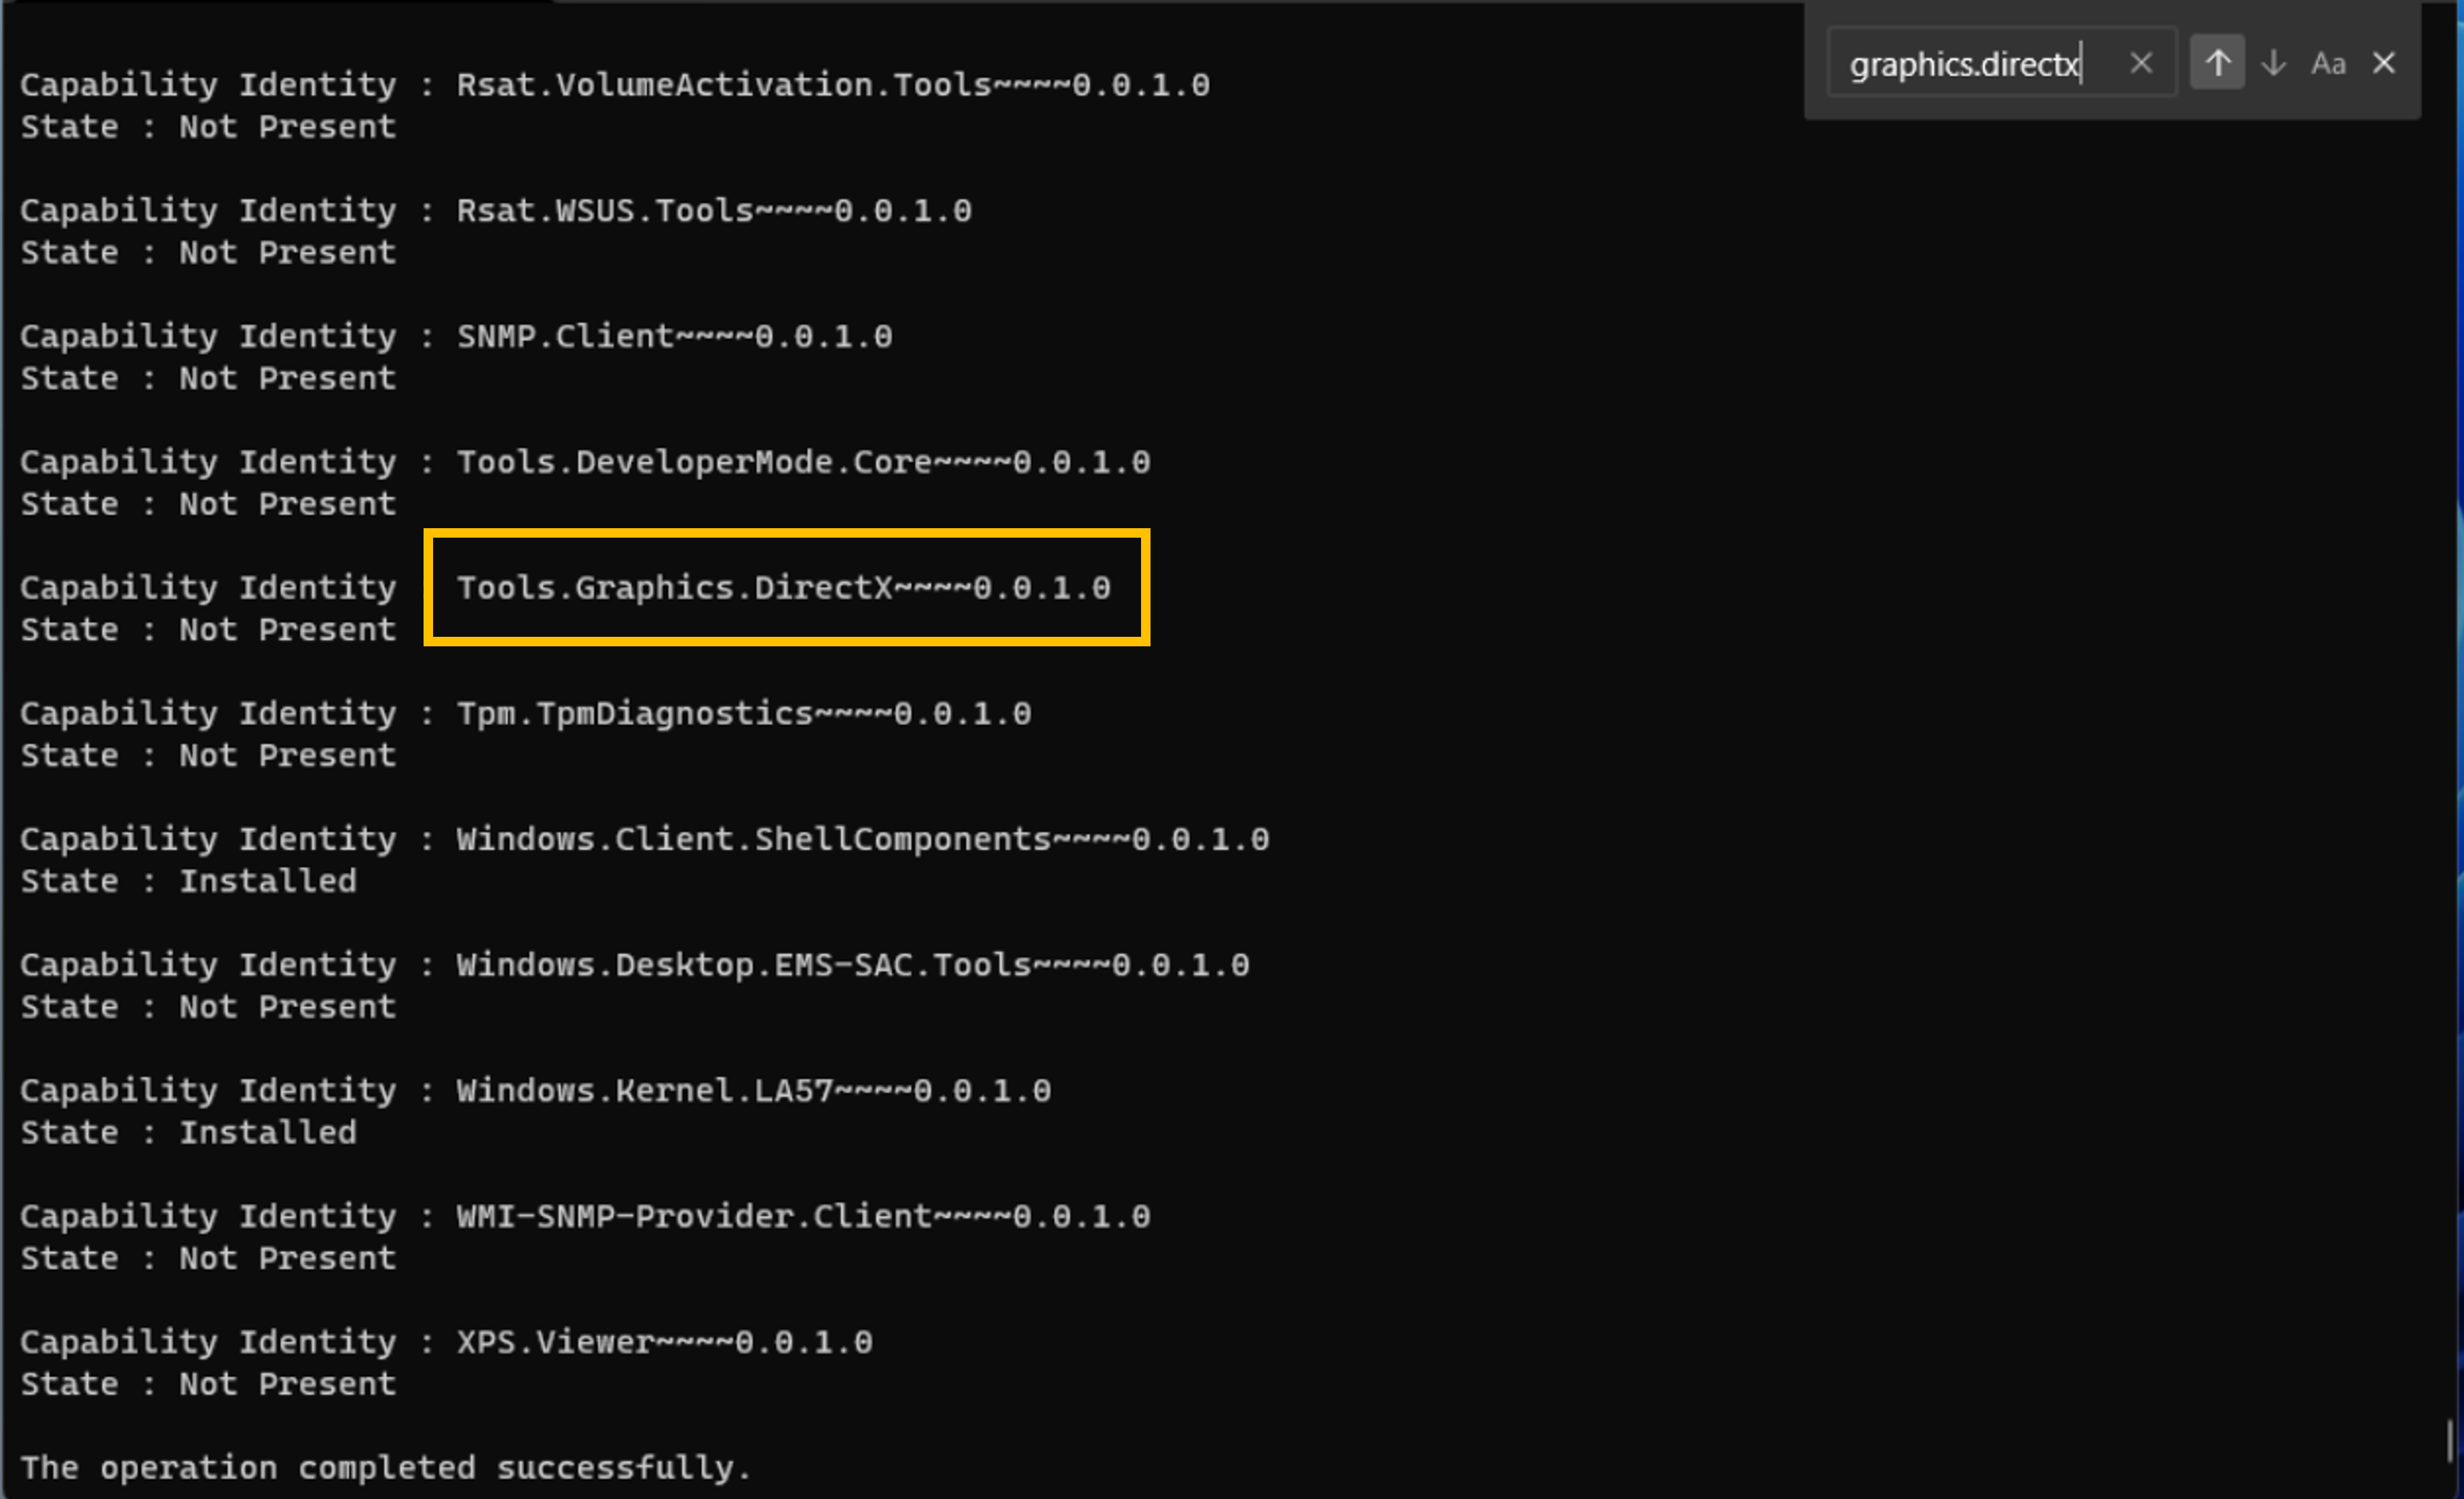
\includegraphics[width=\textwidth]{Images/3/3.Intro.4.3}
            \caption*{\lr{dism /online /Get-Capabilities}}
        \end{figure}

        از لیست نشان داده شده، موردی را که با \lr{\grayBox{Tools.Graphics.DirectX}} شروع می‌شود را پیدا کرده و نام کامل آن را کپی کنید. (ممکن است اعداد مقابل آن با عکس متفاوت باشد)
        سپس دستور زیر را وارد کنید و به جای \lr{\grayBox{<Name>}}، نامی که کپی کردید را قرار دهید:

        \begin{flushleft}
            \grayBox{Dism /Online /Add-Capability /CapabilityName:<Name>}
        \end{flushleft}

        به عنوان مثال:

        \begin{flushleft}
            \normalsize
            \grayBox{Dism /Online /Add-Capability /CapabilityName:Tools.Graphics.DirectX\textasciitilde\textasciitilde\textasciitilde\textasciitilde0.0.1.0}
        \end{flushleft}

        \begin{figure}[H]
            \centering
            \setlength{\belowcaptionskip}{-10pt}
            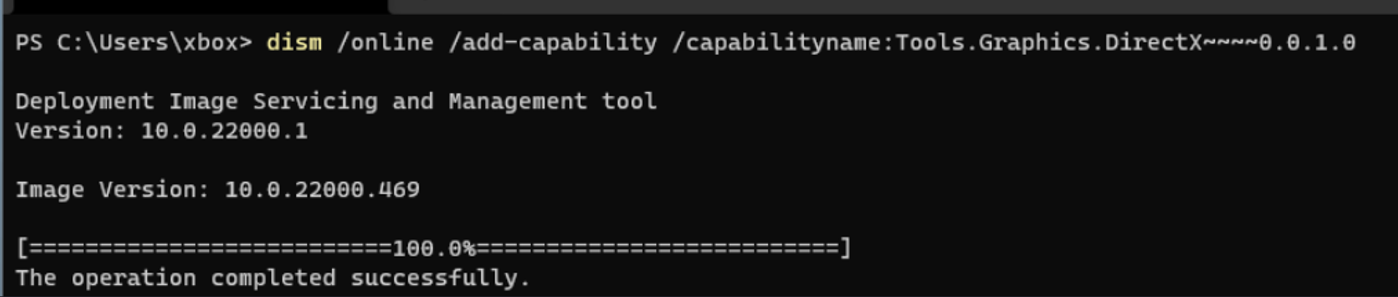
\includegraphics[width=\textwidth]{Images/3/3.Intro.4.4}
            \caption*{\lr{Dism /Online /Add-Capability /CapabilityName:Tools.Graphics.DirectX\textasciitilde\textasciitilde\textasciitilde\textasciitilde0.0.1.0}}
        \end{figure}
    \end{spacing}
}
\textbf{\vspace{-10pt}}

\begin{theo}{thm:pythagoras}
{
    \Large
    دقت کنید که فرآیند نصب ممکن است زمان بر باشد. همچنین دستورات \lr{Dism} به بزرگ و کوچک بودن حروف حساس نیستند.
}
\end{theo}

\textbf{\vspace{-30pt}}
\title{
    \LARGE
    \rullCenterTextWithLine{\textbf{یک پروژه جدید ایجاد کنید}}
}
\textbf{\vspace{-10pt}}

{
    \Large
    \begin{spacing}{1.5}
        ابتدا \lr{Visual Studio 2022} را اجرا کنید، میتوانید با انتخاب \lr{Create a new project} یک پروژه ی جدید بسازید (شکل \ref{fig:3.Intro.5.1}) یا به منوی اصلی بروید و \lr{File->New->Project} را انتخاب کنید (شکل \ref{fig:3.Intro.5.2}).
        پنجره ی \lr{New Project} ظاهر می شود (شکل \ref{fig:3.Intro.5.3}).
        از قسمت بالا \lr{C++} و \lr{Windows} را انتخاب کنید و روی \lr{Empty Project} مانند شکل کلیک کرده و \lr{Next} را بزنید.
        در مرحله بعد به پروژه یک نام بدهید و مکانی را که می خواهید دایرکتوری پروژه در آن ذخیره شود را مشخص کنید (شکل \ref{fig:3.Intro.5.4}).
        حالا \lr{Create} را بزنید.

        \begin{figure}[H]
            \centering
            \setlength{\belowcaptionskip}{-10pt}
            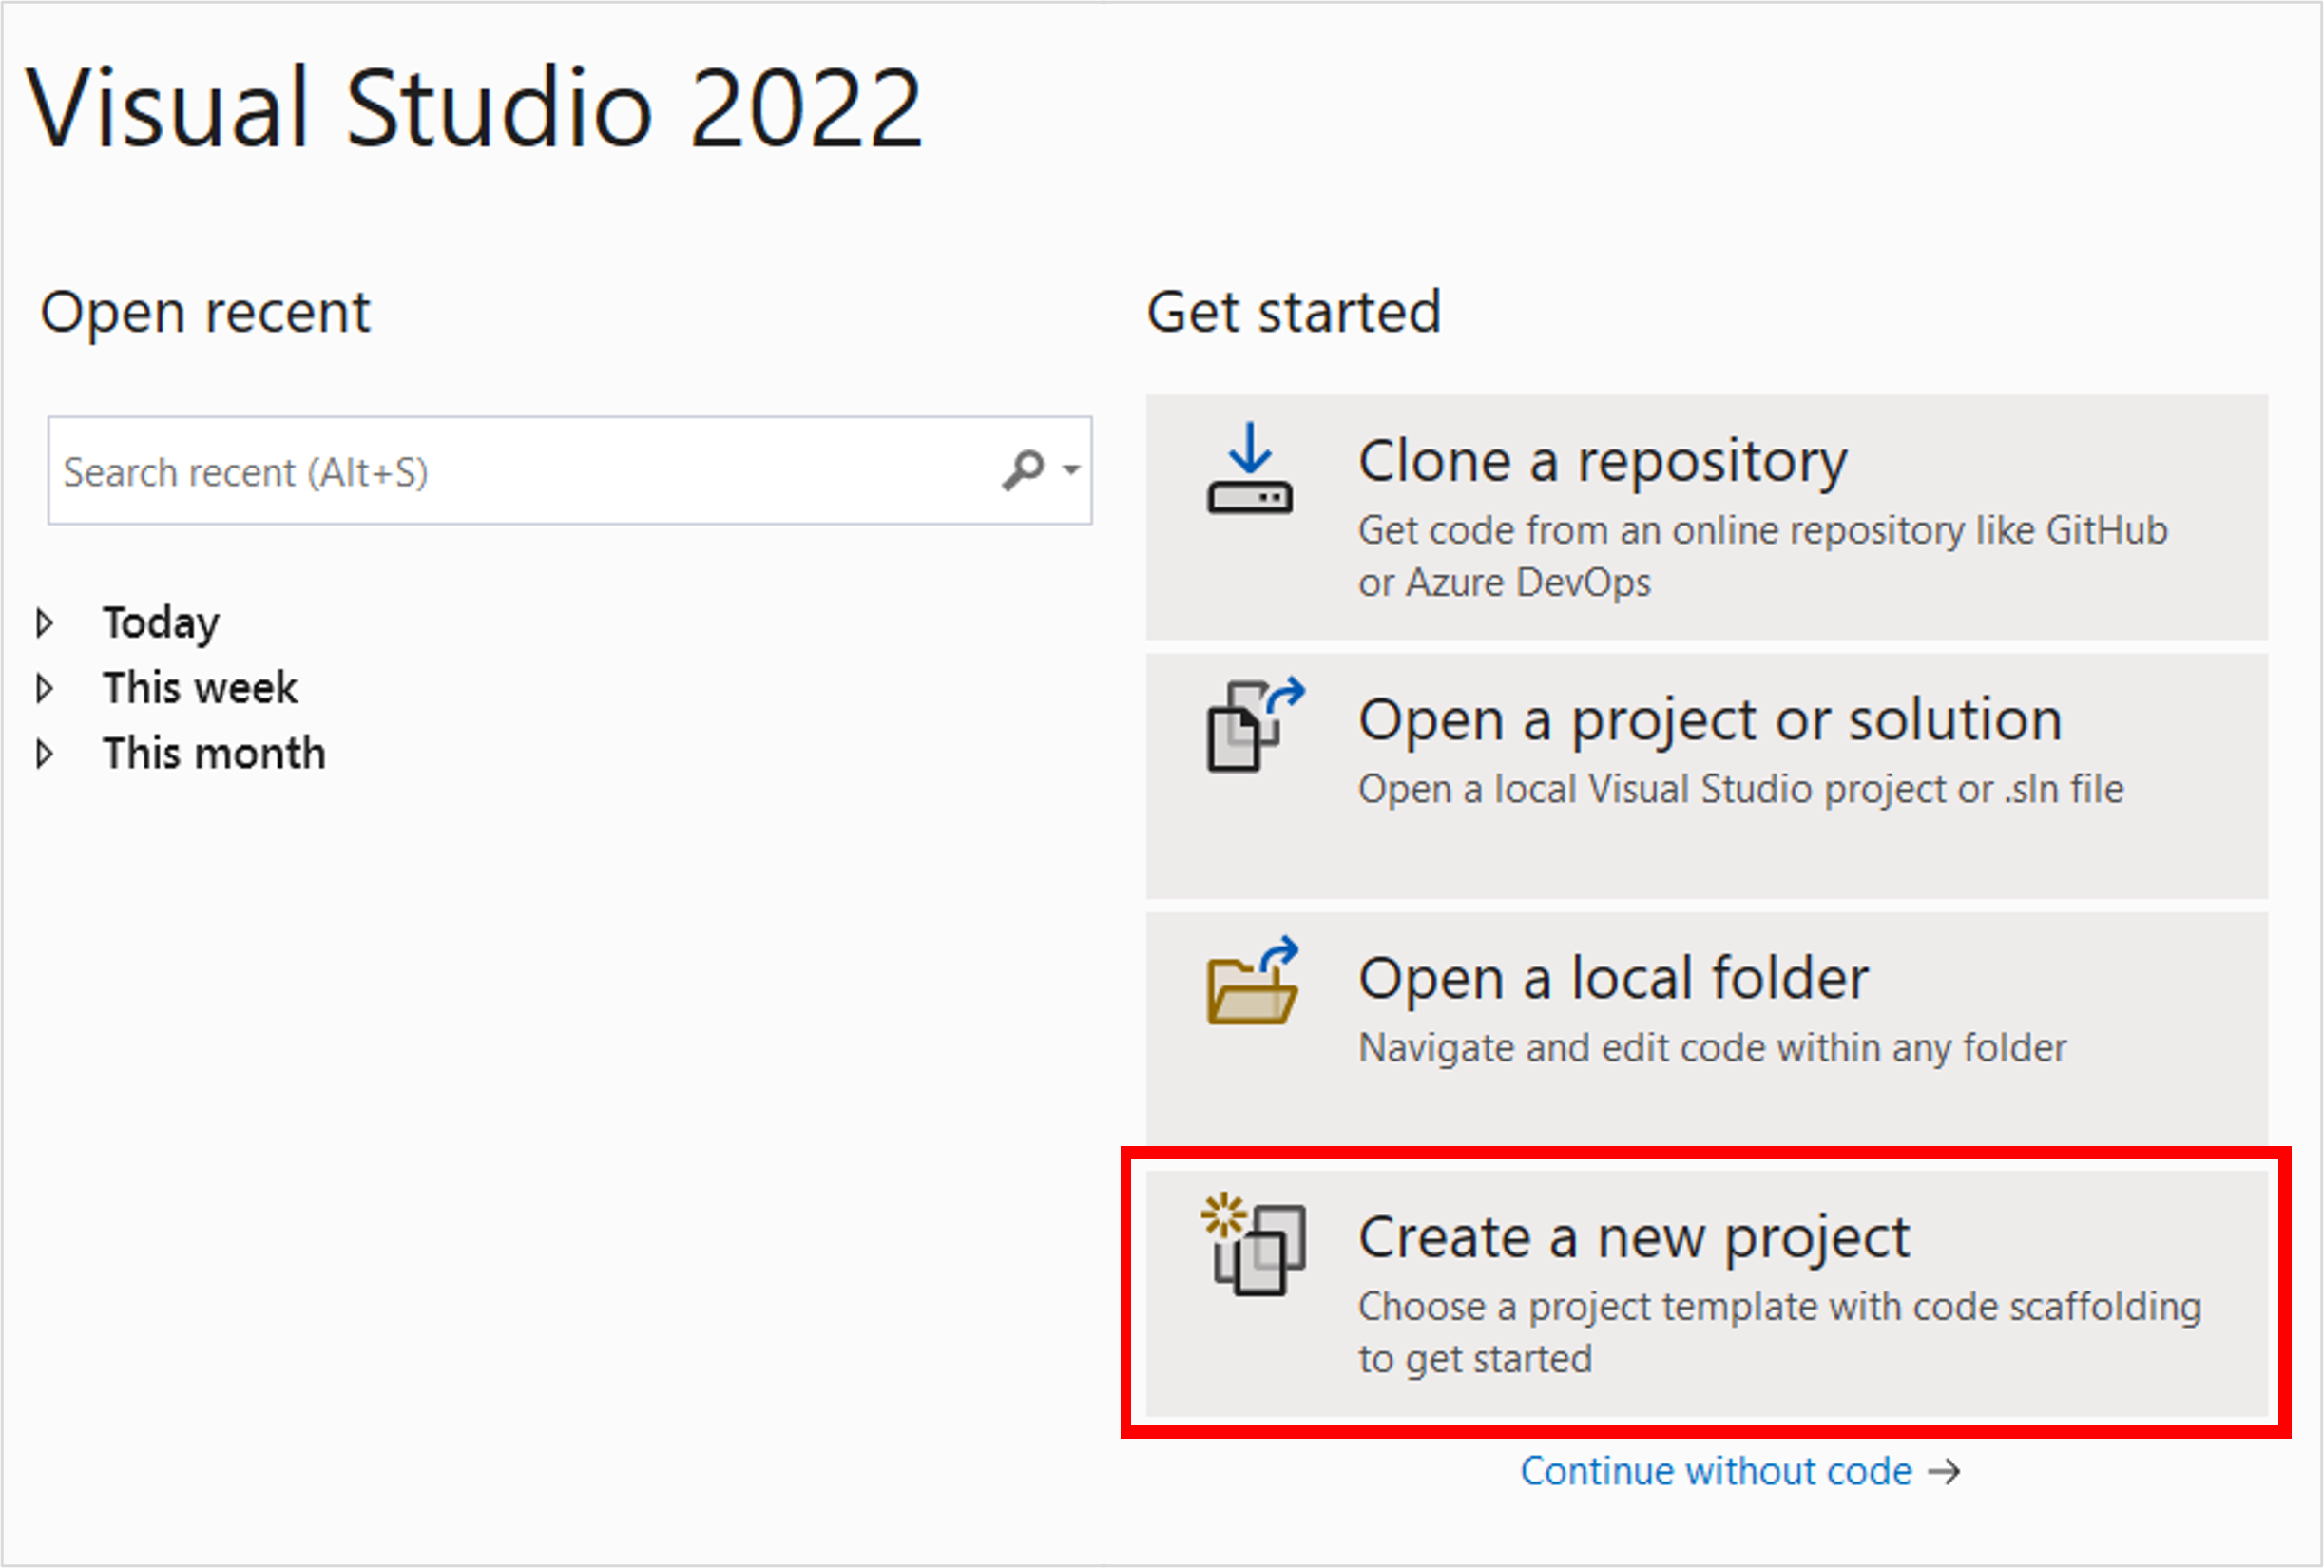
\includegraphics[width=\textwidth]{Images/3/3.Intro.5.1}
            \caption{انتخاب \lr{Create a new project}}
            \label{fig:3.Intro.5.1}
        \end{figure}

        \begin{figure}[H]
            \centering
            \setlength{\belowcaptionskip}{-10pt}
            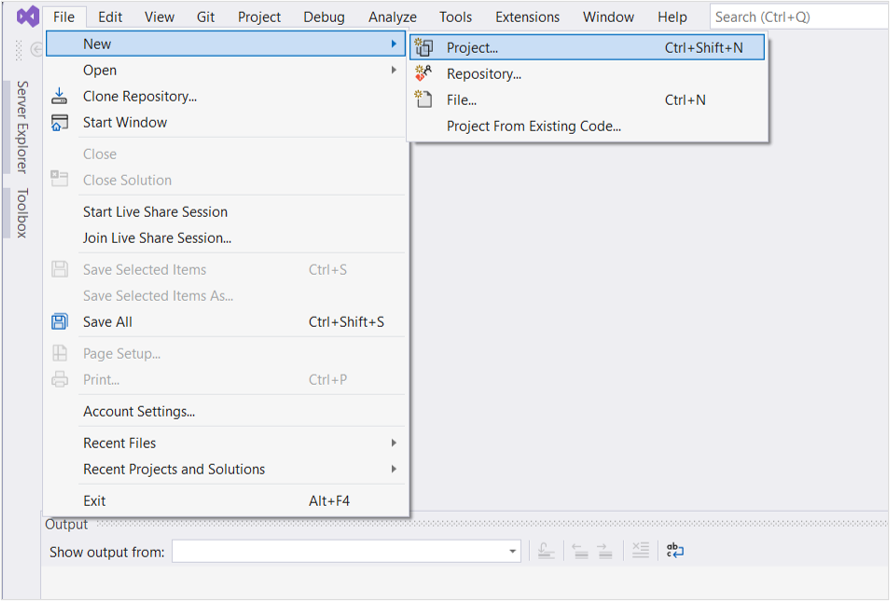
\includegraphics[width=\textwidth]{Images/3/3.Intro.5.2}
            \caption{انتخاب \lr{New Project}}
            \label{fig:3.Intro.5.2}
        \end{figure}

        \begin{figure}[H]
            \centering
            \setlength{\belowcaptionskip}{-10pt}
            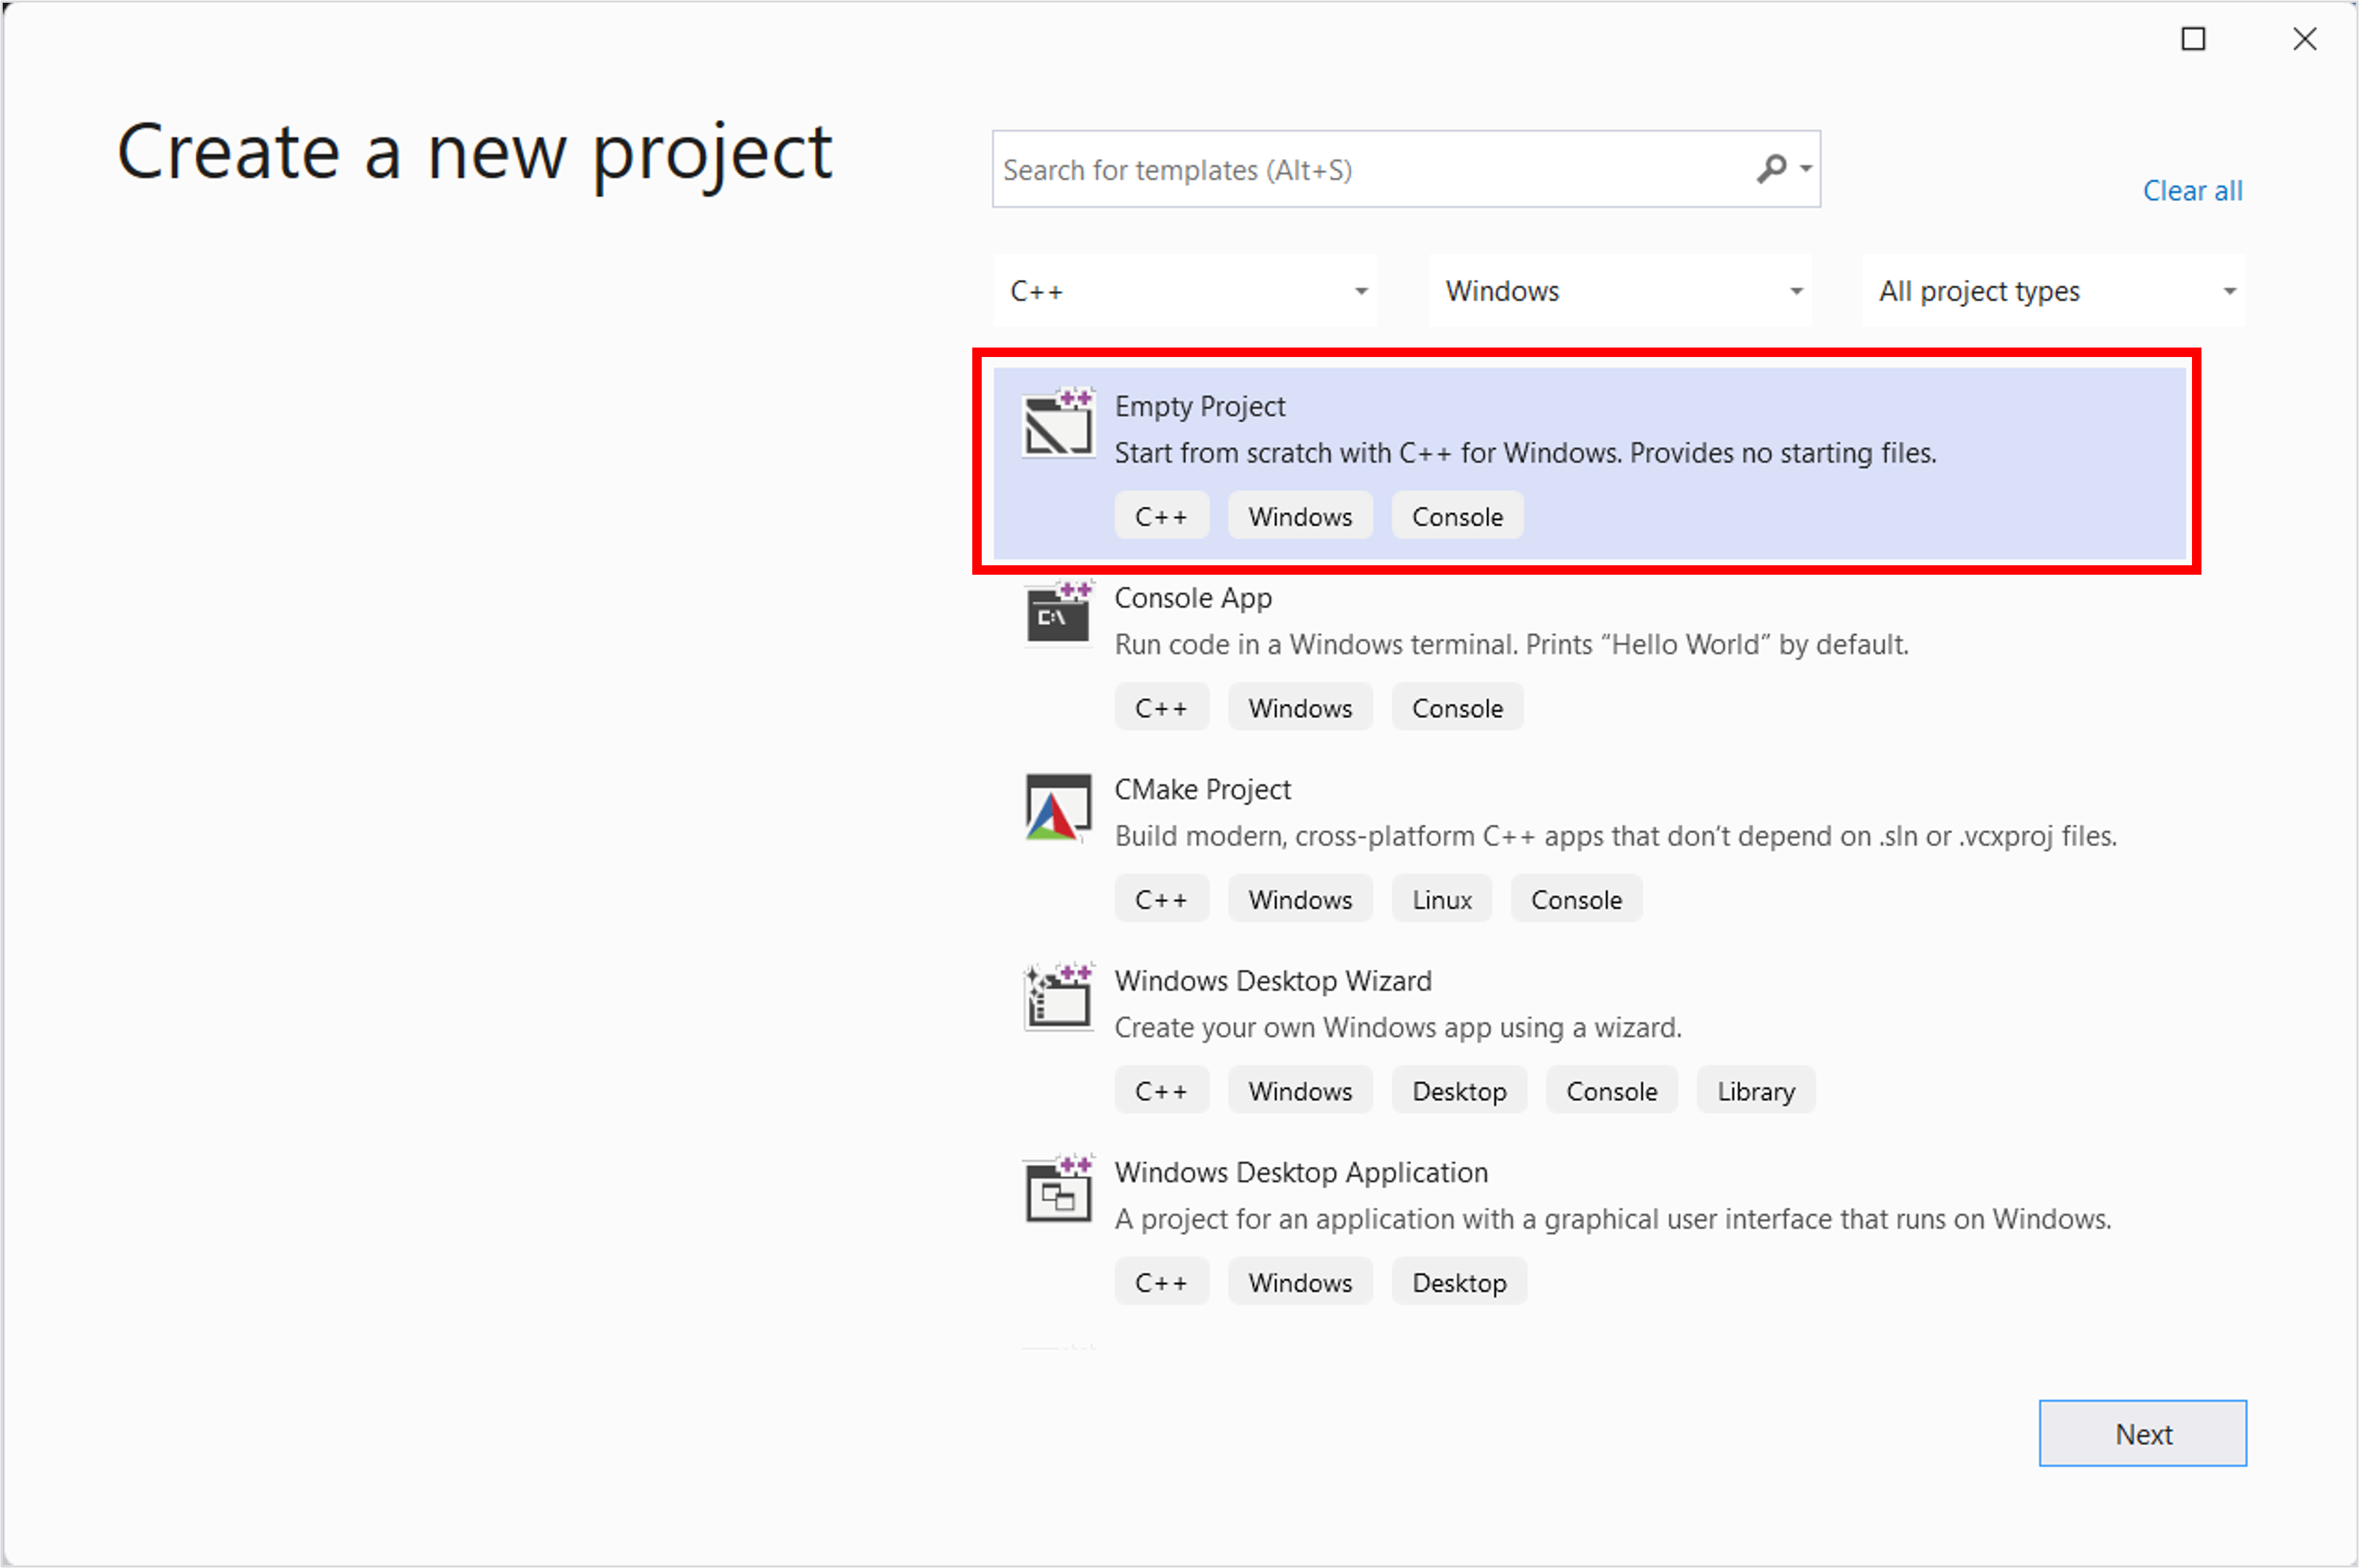
\includegraphics[width=\textwidth]{Images/3/3.Intro.5.3}
            \caption{انتخاب \lr{Empty C++ Project}}
            \label{fig:3.Intro.5.3}
        \end{figure}

        \begin{figure}[H]
            \centering
            \setlength{\belowcaptionskip}{-10pt}
            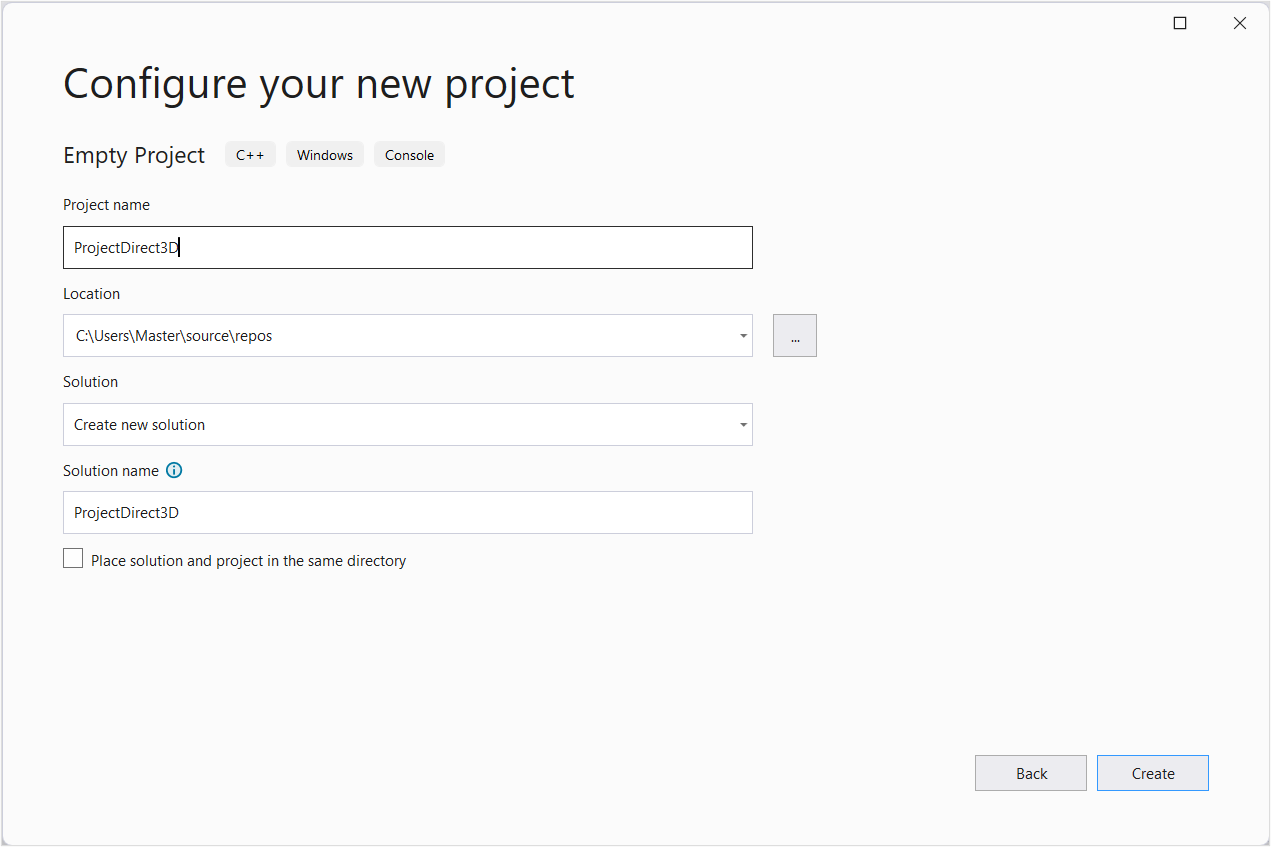
\includegraphics[width=\textwidth]{Images/3/3.Intro.5.4}
            \caption{پنجره \lr{Configure new project}}
            \label{fig:3.Intro.5.4}
        \end{figure}

        اکنون در پنجره ی باز شده، از قسمت \lr{Solution Explorer} ، روی نام پروژه کلیک راست کرده و \lr{Properties} را بزنید (شکل \ref{fig:3.Intro.5.5}).

        \begin{figure}[H]
            \centering
            \setlength{\belowcaptionskip}{-10pt}
            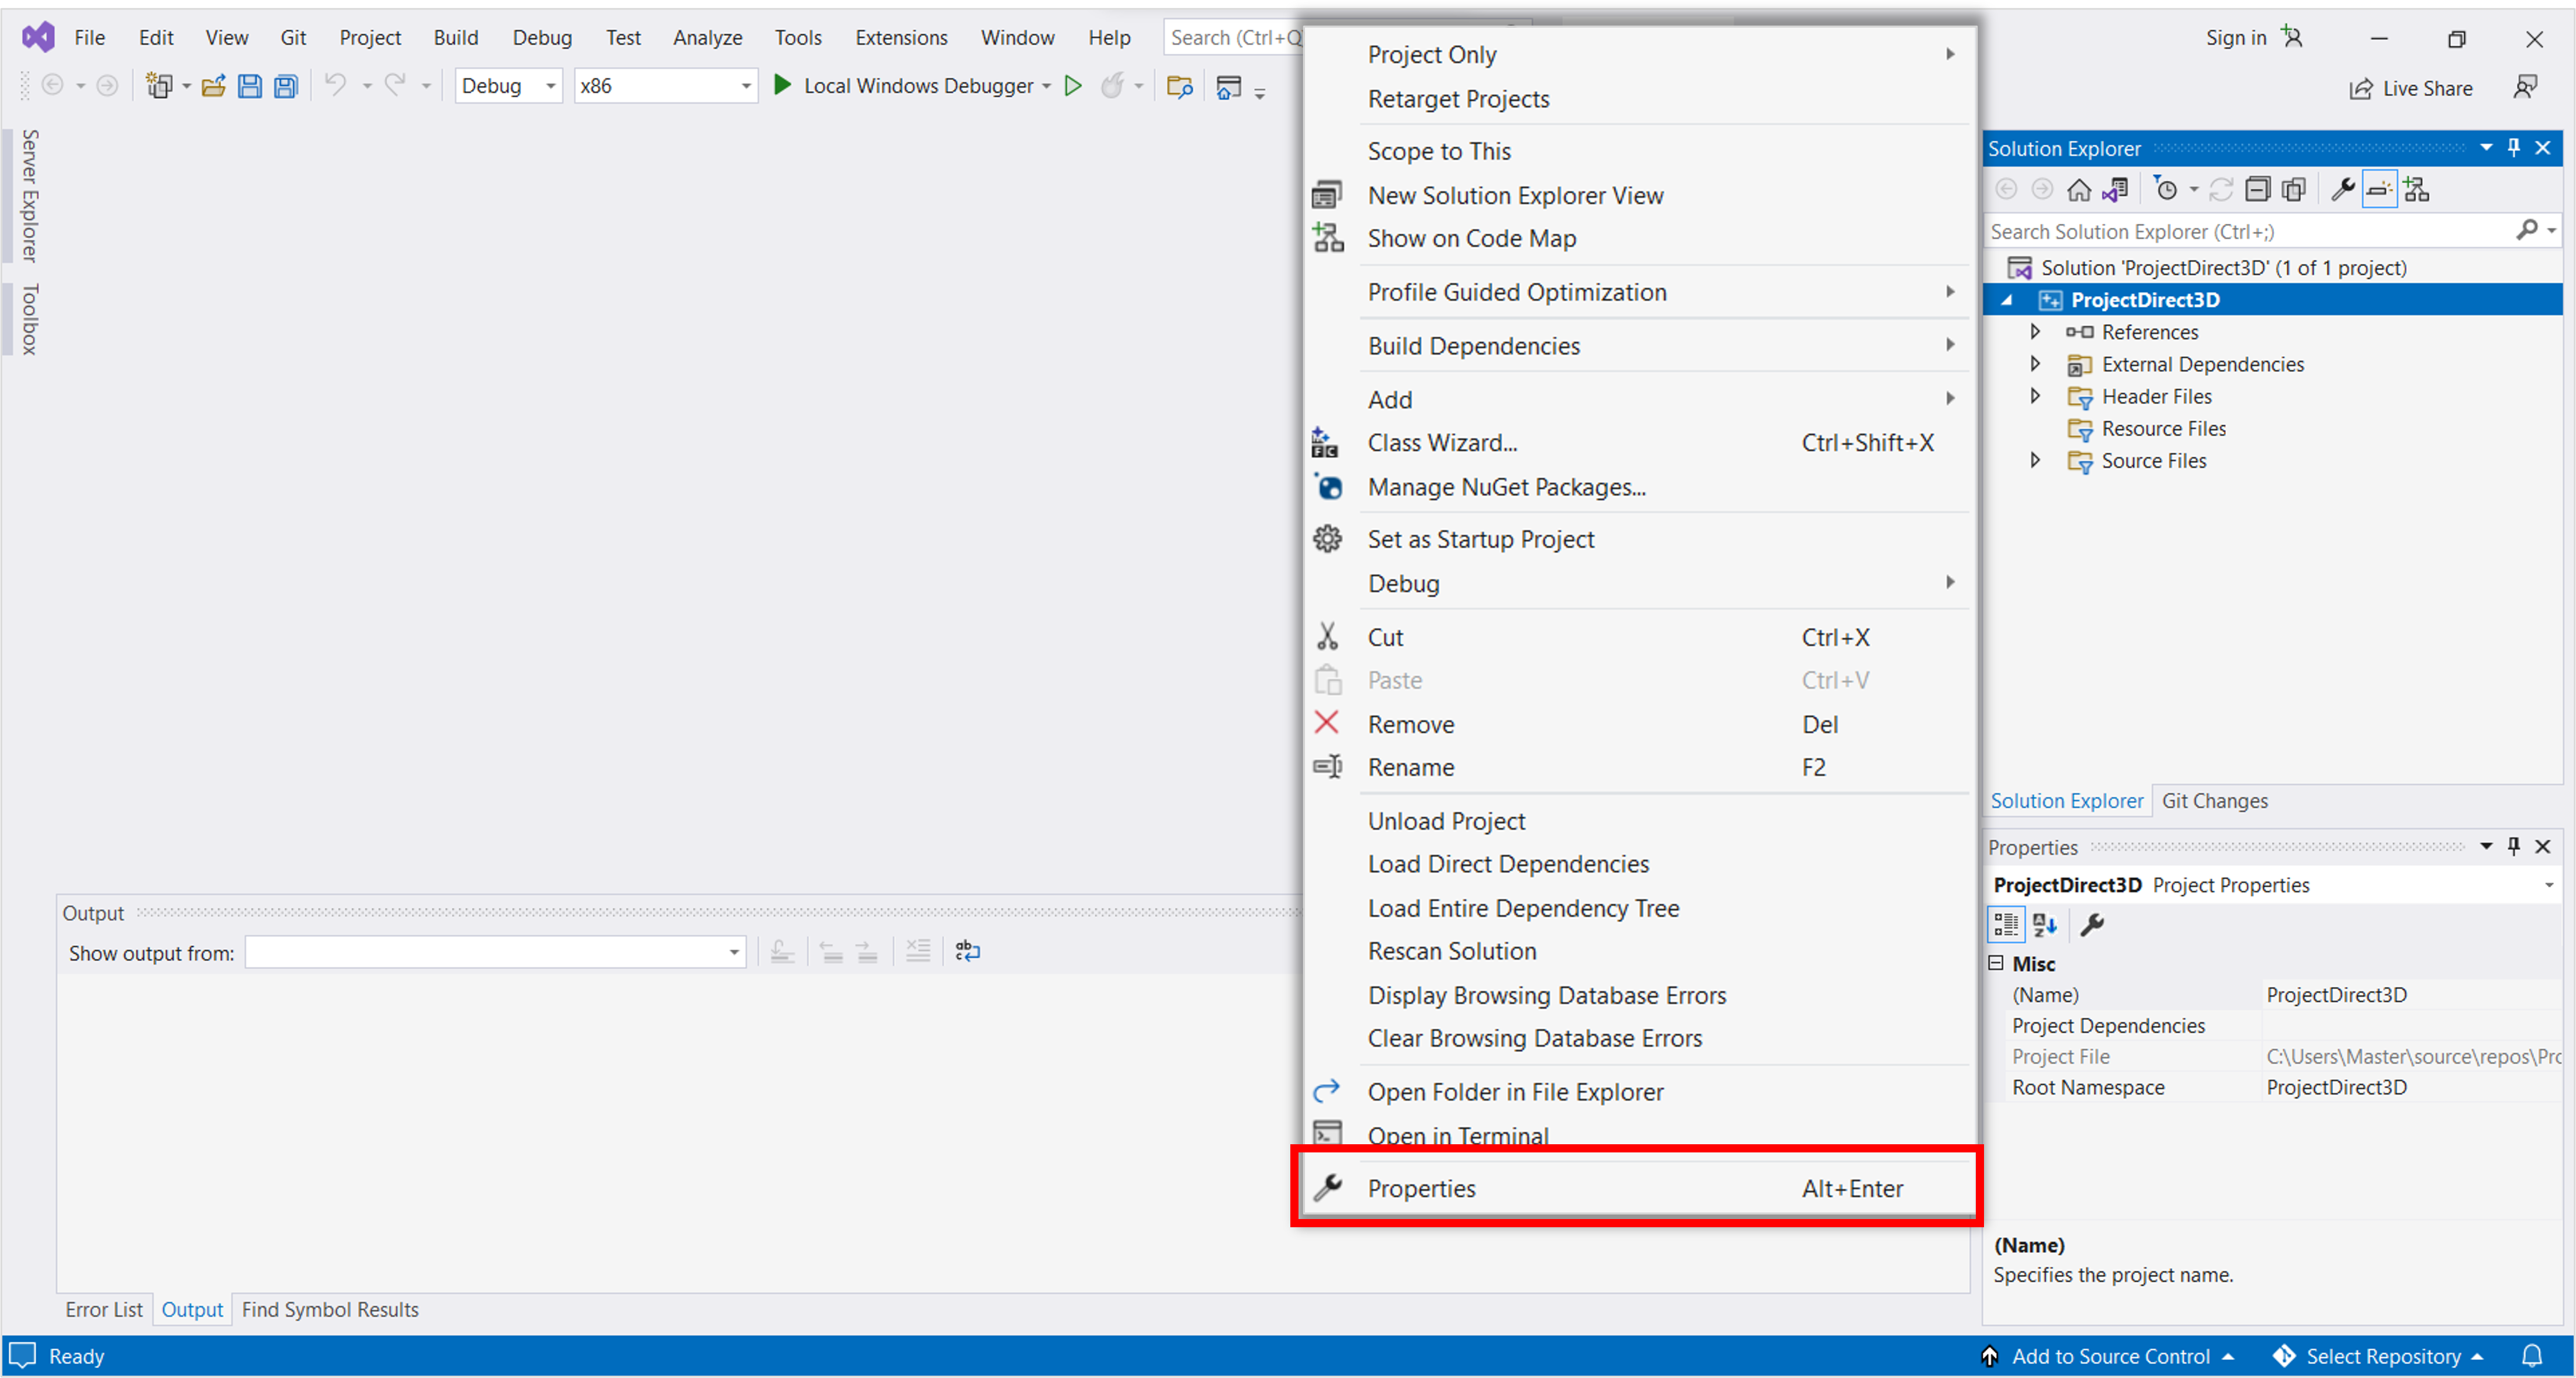
\includegraphics[width=\textwidth]{Images/3/3.Intro.5.5}
            \caption{\lr{Poject Properties}}
            \label{fig:3.Intro.5.5}
        \end{figure}

        در پنجره ی باز شده باید تغییراتی را اعمال کنید،
        ابتدا از قسمت بالای پنجره \lr{Win32} را انتخاب کنید (شکل \ref{fig:3.Intro.5.6}) و بررسی کنید که مقادیر پنجره ی شما با عکس یکسان است.

        \begin{figure}[H]
            \centering
            \setlength{\belowcaptionskip}{-10pt}
            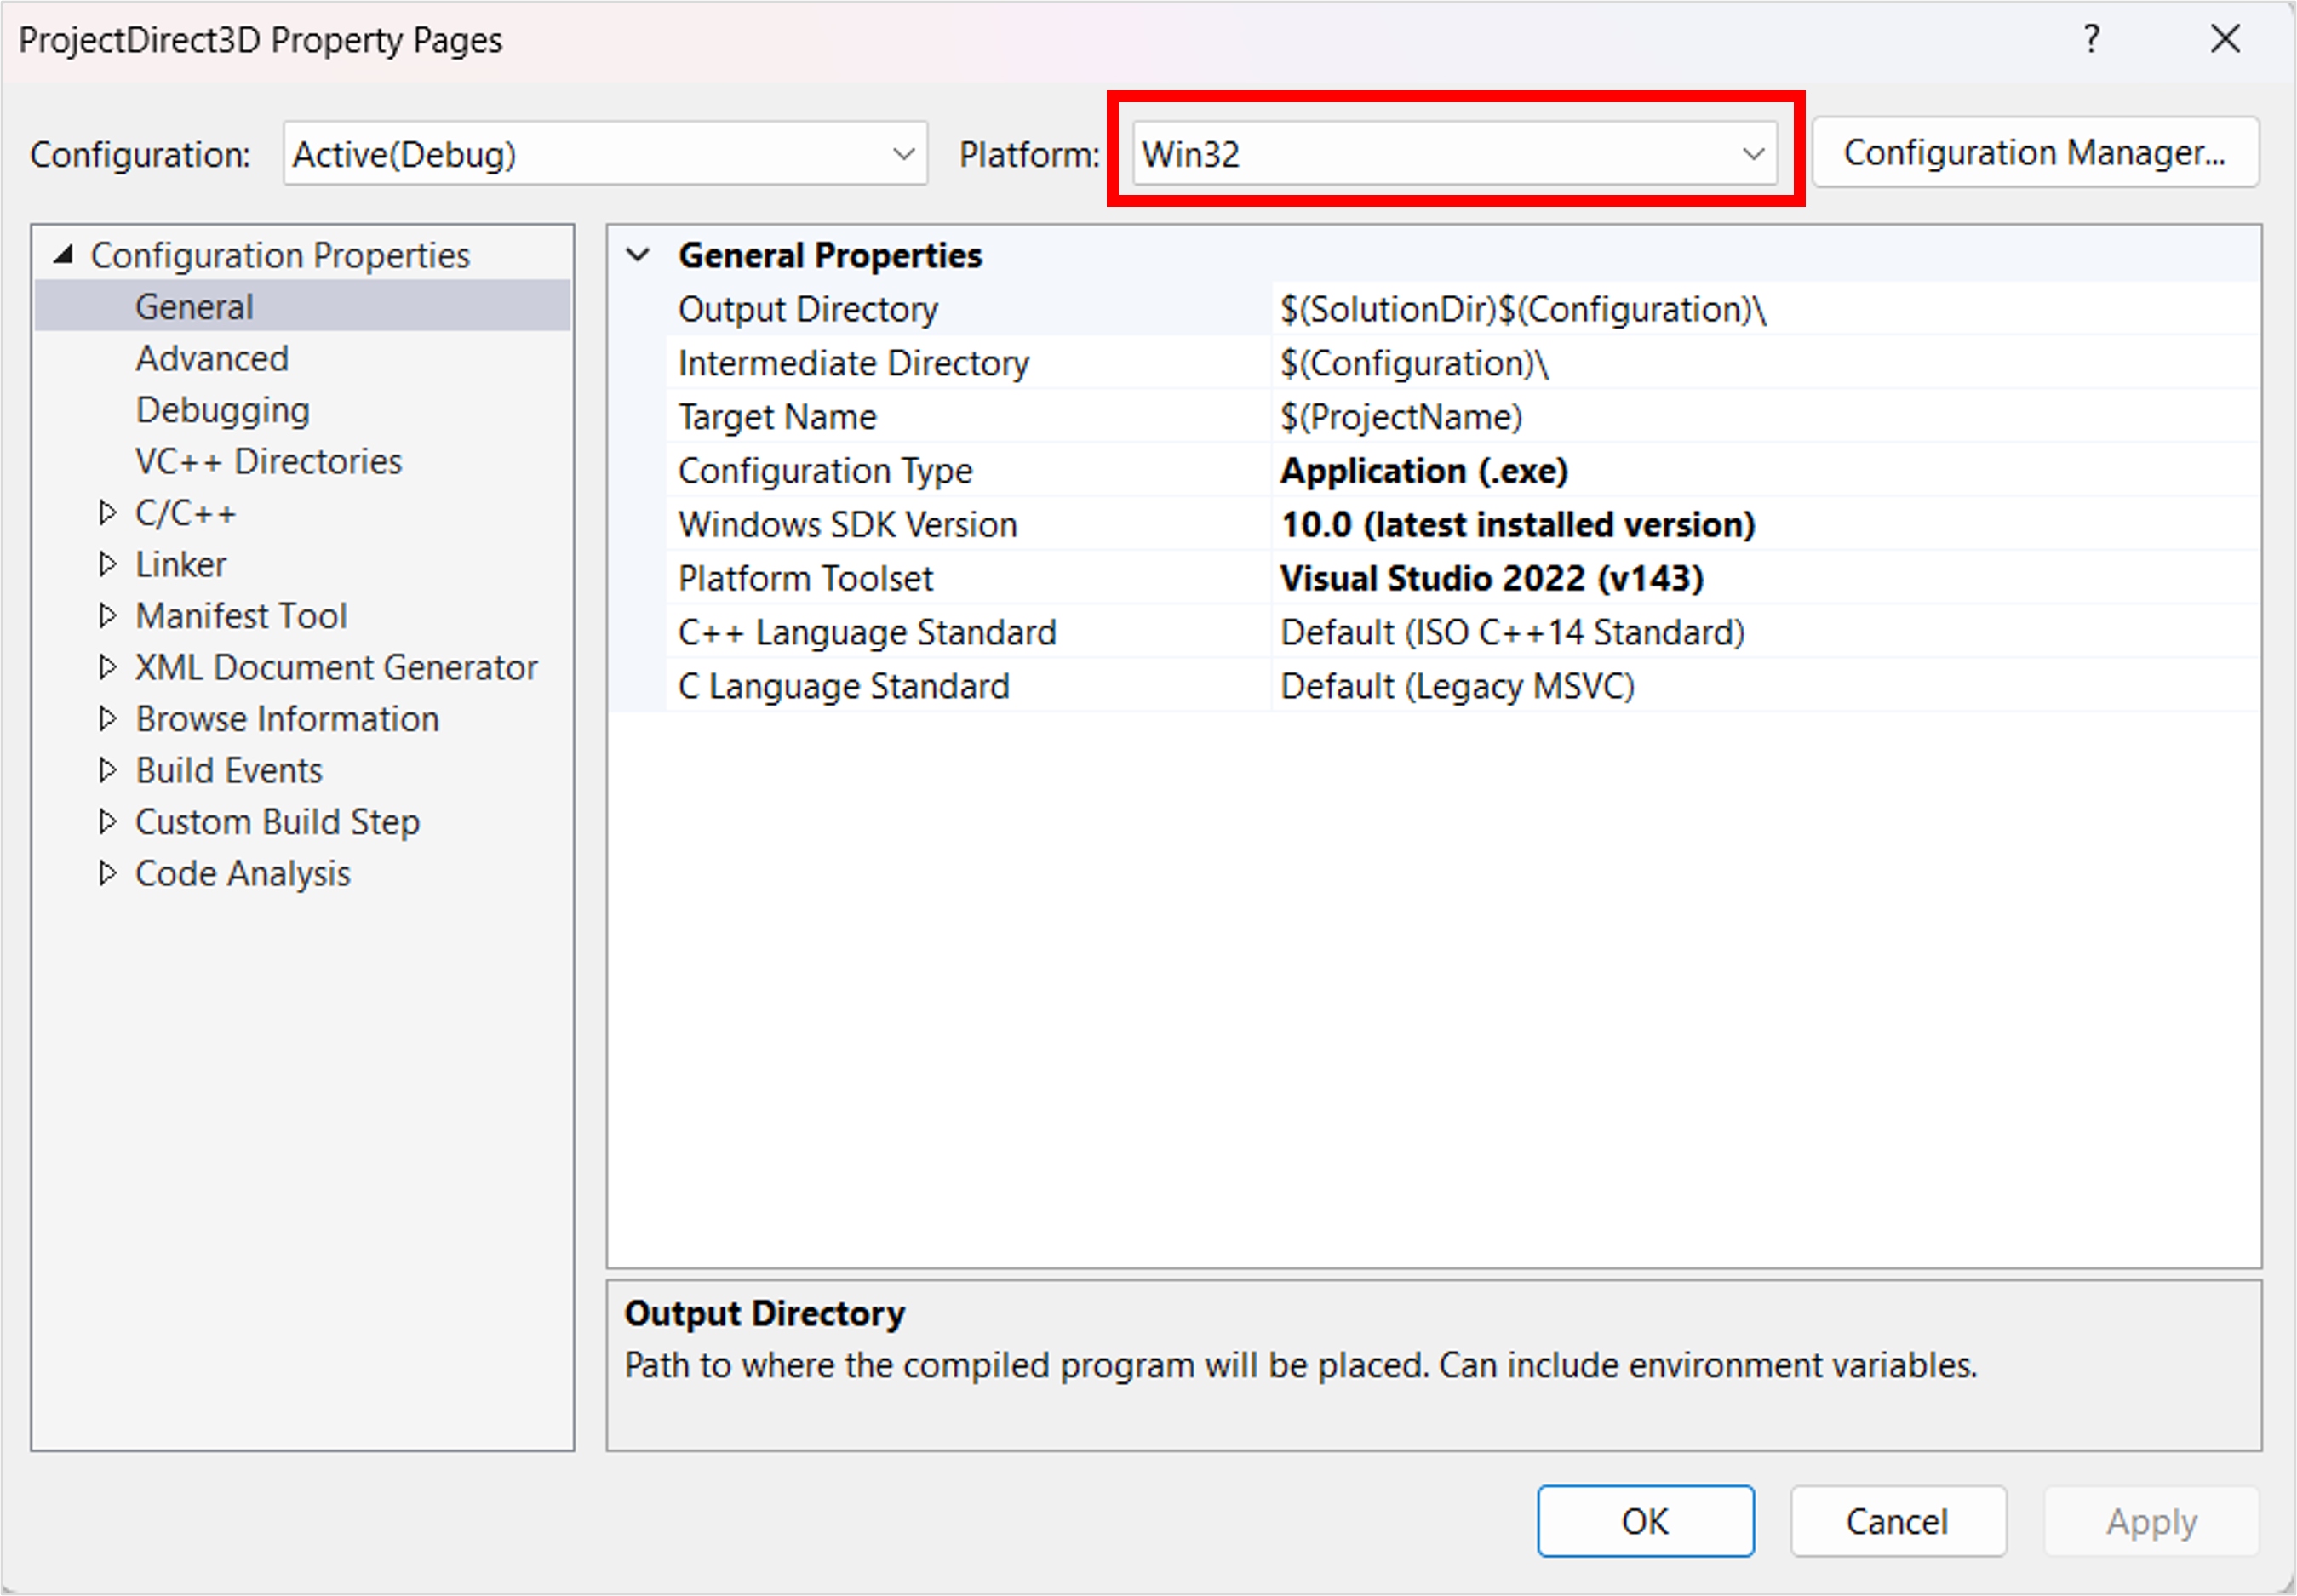
\includegraphics[width=\textwidth]{Images/3/3.Intro.5.6}
            \caption{پنجره \lr{Property Page}}
            \label{fig:3.Intro.5.6}
        \end{figure}

        سپس زیر درخت \lr{Linker->System} را انتخاب کنید و در سمت راست \lr{SubSystem} را روی \lr{Windows (/SUBSYSTEM:WINDOWS)} قرار دهید (شکل \ref{fig:3.Intro.5.7}).

        \begin{figure}[H]
            \centering
            \setlength{\belowcaptionskip}{-10pt}
            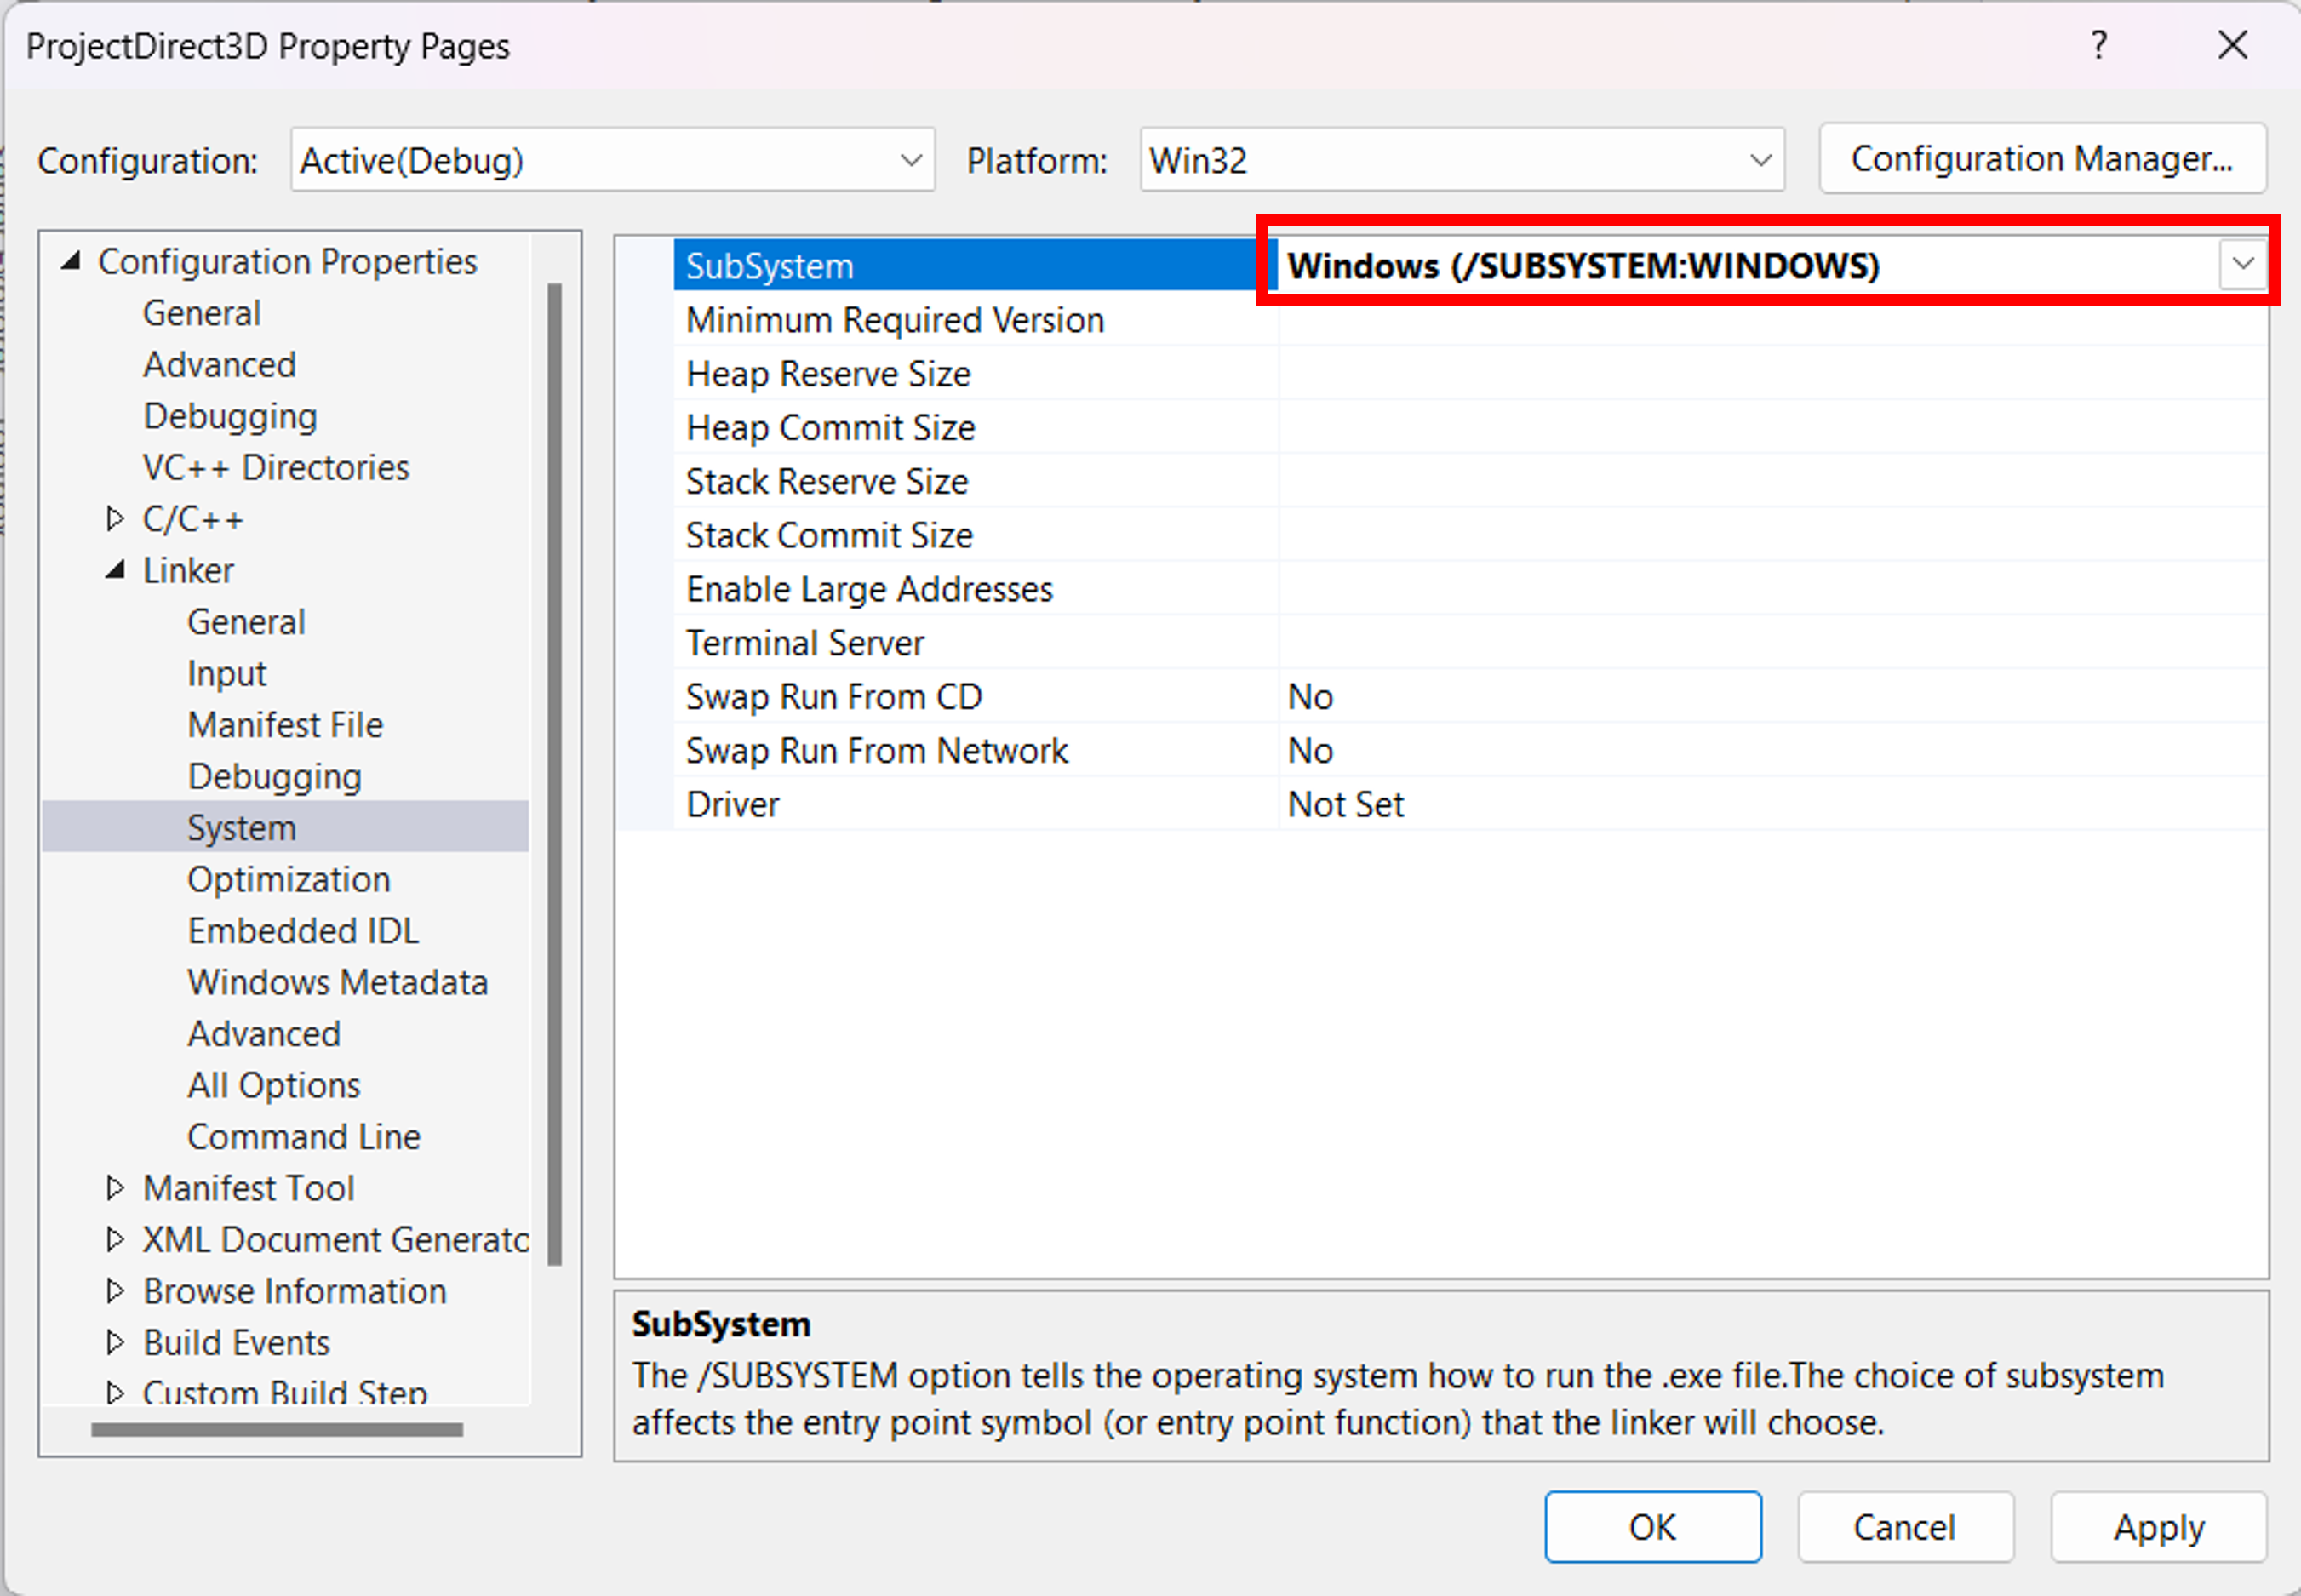
\includegraphics[scale=0.7]{Images/3/3.Intro.5.7}
            \caption{تنظیمات \lr{Linker System}}
            \label{fig:3.Intro.5.7}
        \end{figure}
    \end{spacing}
}

\textbf{\vspace{-30pt}}
\title{
    \LARGE
    \rullCenterTextWithLine{\textbf{اضافه کردن کد منبع و \lr{build} کردن پروژه}}
}
\textbf{\vspace{-15pt}}

{
    \Large
    \begin{spacing}{1.3}
        پس از اتمام تنظیمات ، میتوانیم فایل های کد منبع را به پروژه اضافه کرده و آن build کنیم.
        ابتدا پروژه Box یعنی BoxApp.cpp و پوشه Shaders را در فهرست پروژه کپی کنید (شکل \ref{fig:3.Intro.5.8.1}).
        (فایل ها در این مسیر هستند: \lr{d3d12book\symbol{92}Chapter 6 Drawing in Direct3D\symbol{92}Box})

        \begin{figure}[H]
            \centering
            \setlength{\belowcaptionskip}{-10pt}
            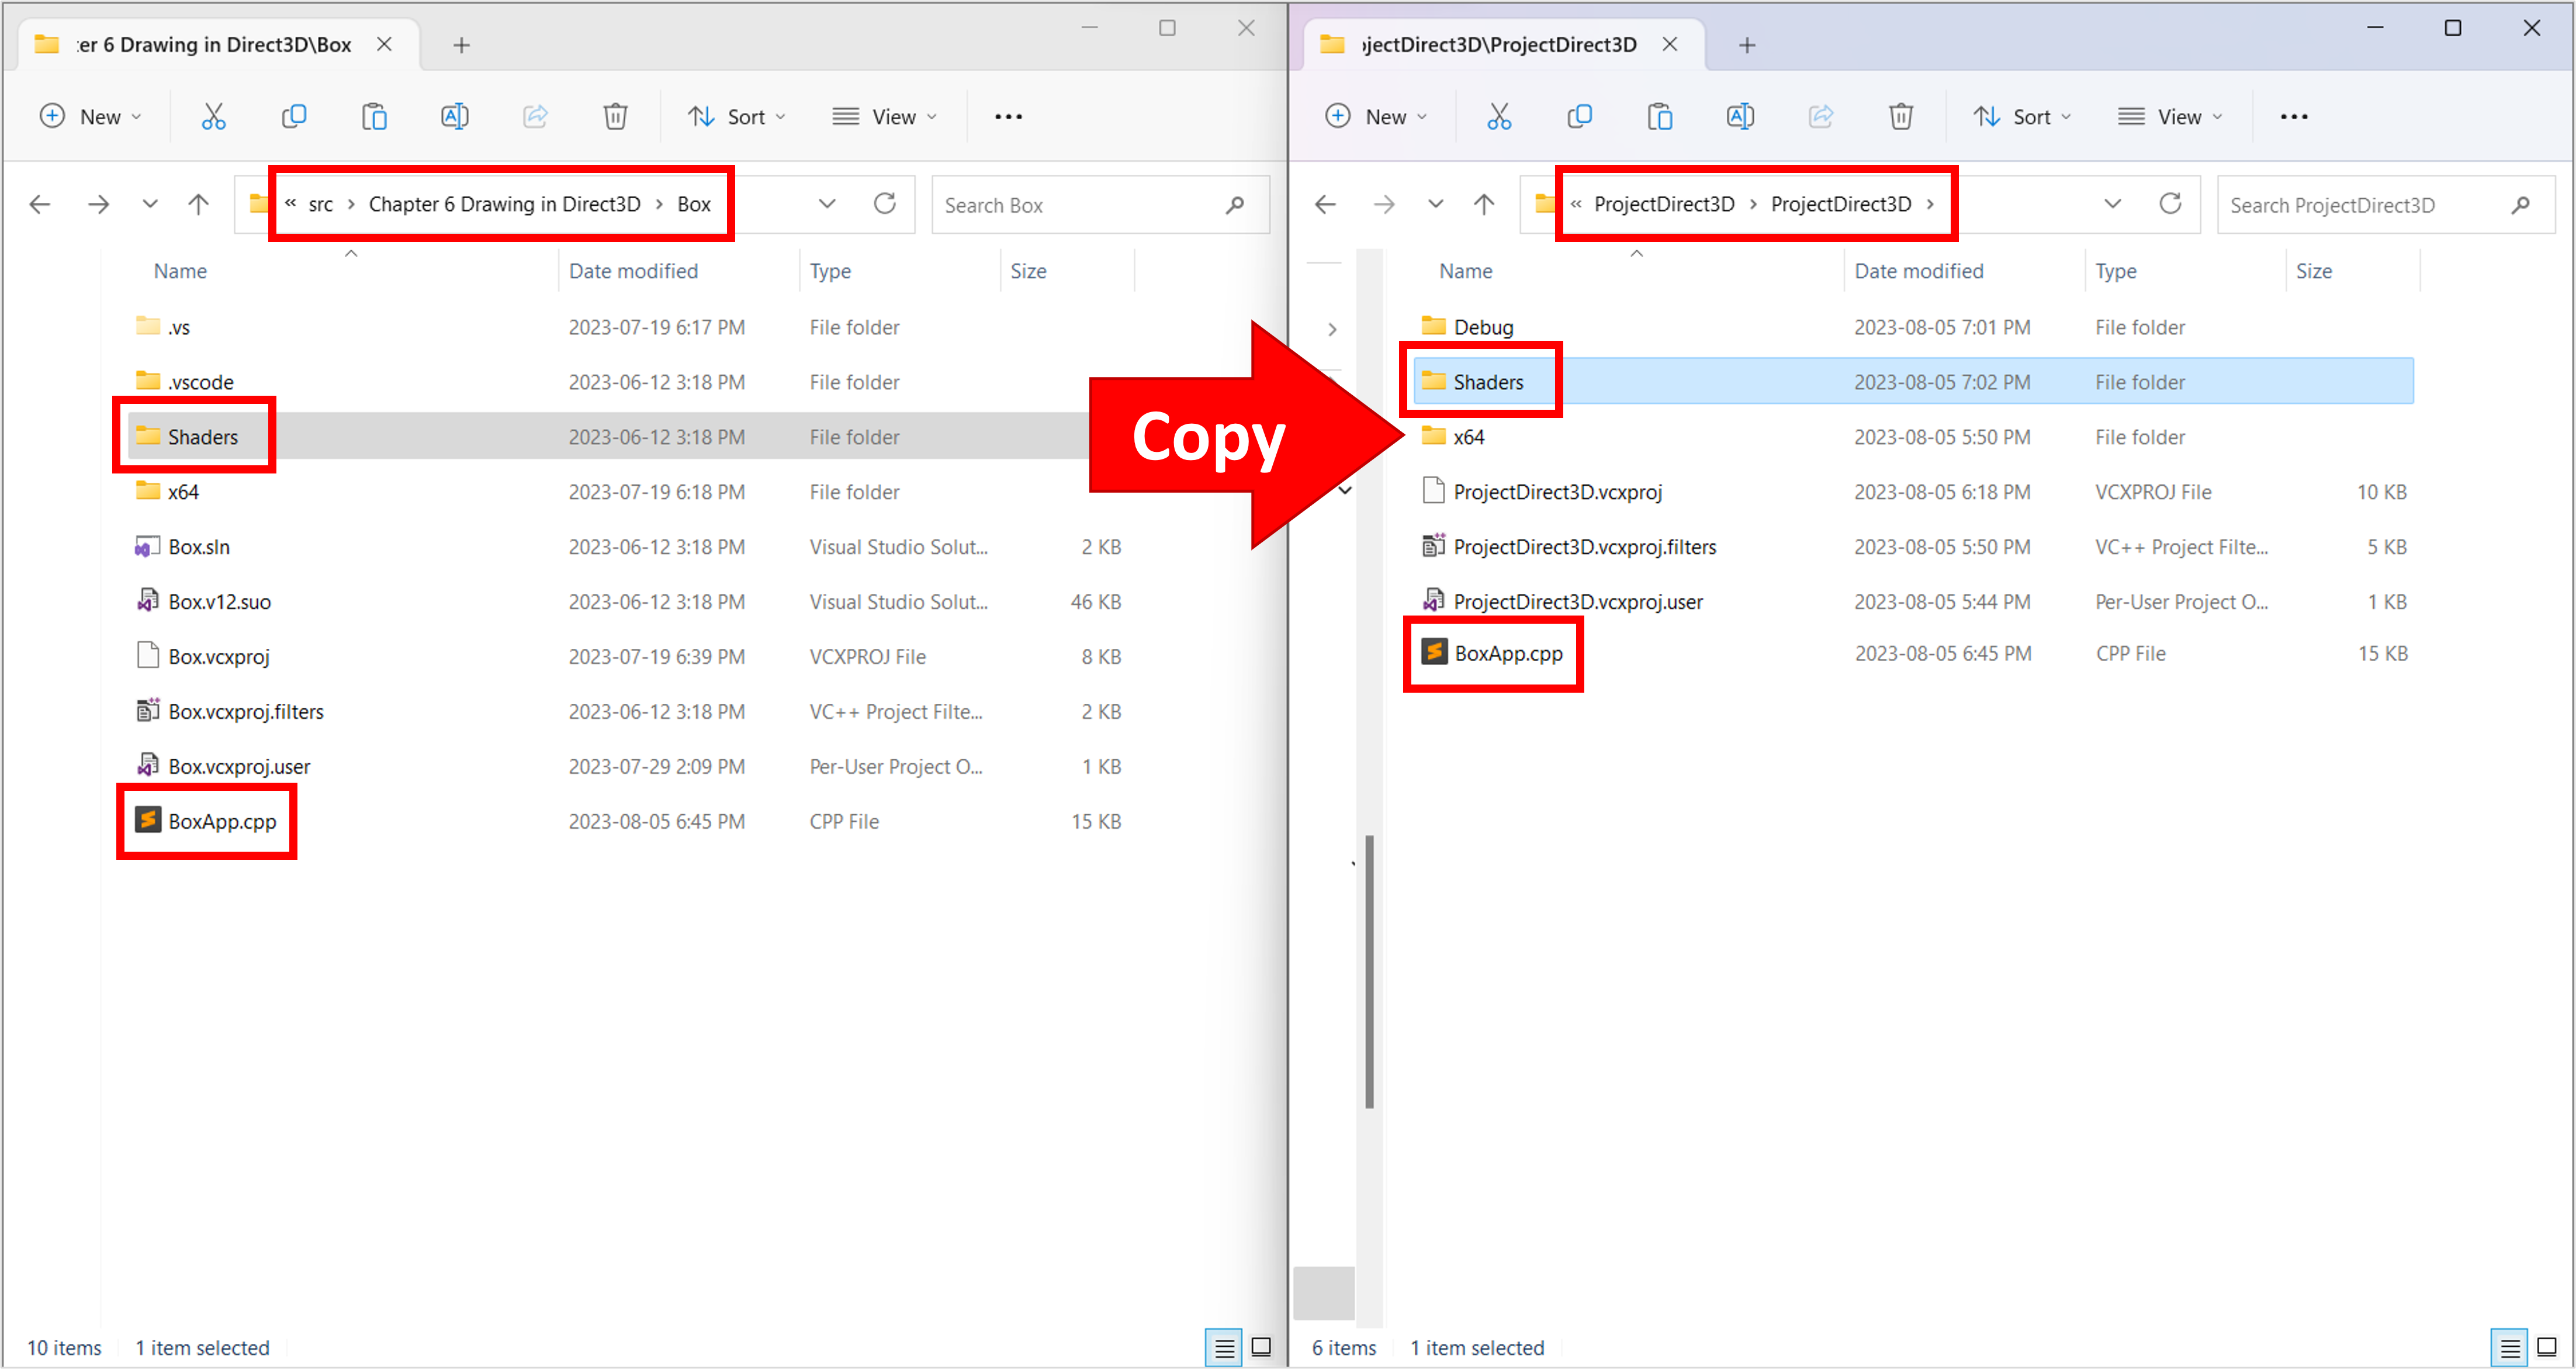
\includegraphics[width=\textwidth]{Images/3/3.Intro.5.8.1}
            \caption{کپی کردن فایل ها}
            \label{fig:3.Intro.5.8.1}
        \end{figure}

        \begin{theo}{thm:pythagoras}
        {
            \Large
            در صورتی که هنگام اجرا با ارور زیر مواجه شدید ، موارد بالا را به درستی انجام نداده اید و باید بار دیگر آن ها را بررسی کنید.

            \begin{figure}[H]
                \centering
                \setlength{\belowcaptionskip}{-10pt}
                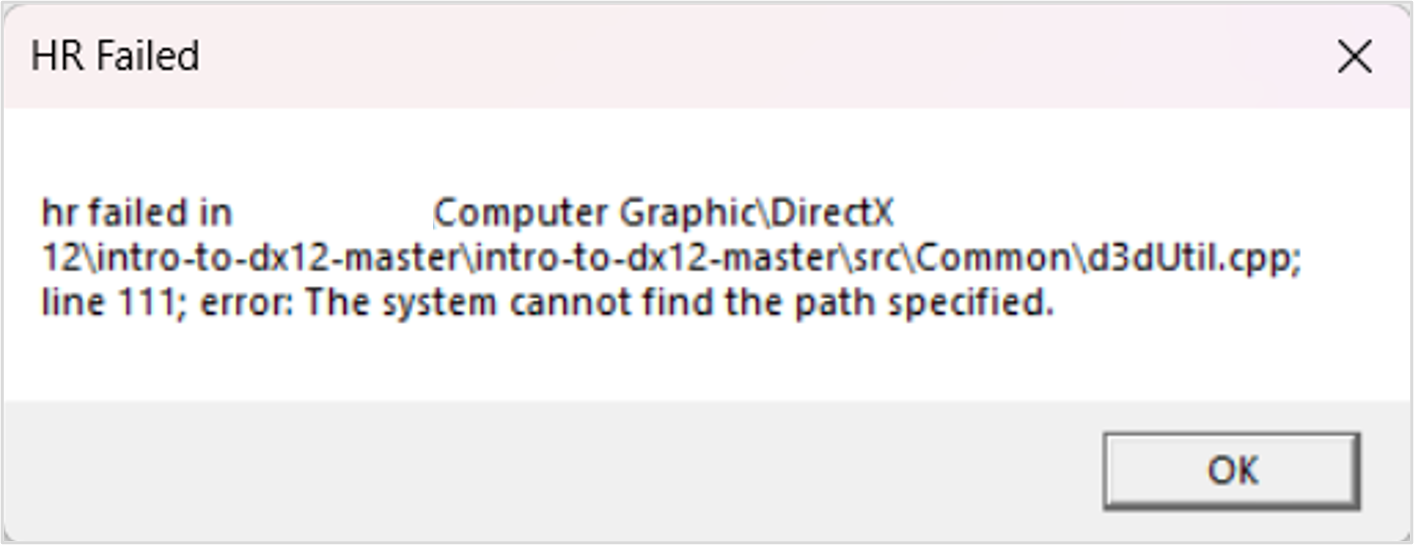
\includegraphics[scale=0.8]{Images/3/3.Intro.5.8.2}
                \caption{ارور \lr{HR Failed} \textbf{\vspace{12pt}}}
                \label{fig:3.Intro.5.8.2}
            \end{figure}
        }
        \end{theo}
        \textbf{\vspace{6pt}}
        بعد از کپی کردن فایل ها، گام های زیر را برای اضافه کردن کد به پروژه دنبال کنید.

        \begin{enumerate}
            \item {در قسمت \lr{Solution Explorer} بر روی نام پروژه کلیک راست کنید و \lr{Add->Exiting Item...} را انتخاب کنید.
            از پنجره ی باز شده \lr{BoxApp.cpp} را انتخاب کنید.   }

            \item {در قسمت \lr{Solution Explorer} بر روی نام پروژه کلیک راست کنید و \lr{Add->Exiting Item...} را انتخاب کنید (شکل \ref{fig:3.Intro.5.9.2}).

                \begin{figure}[H]
                    \centering
                    \setlength{\belowcaptionskip}{-10pt}
                    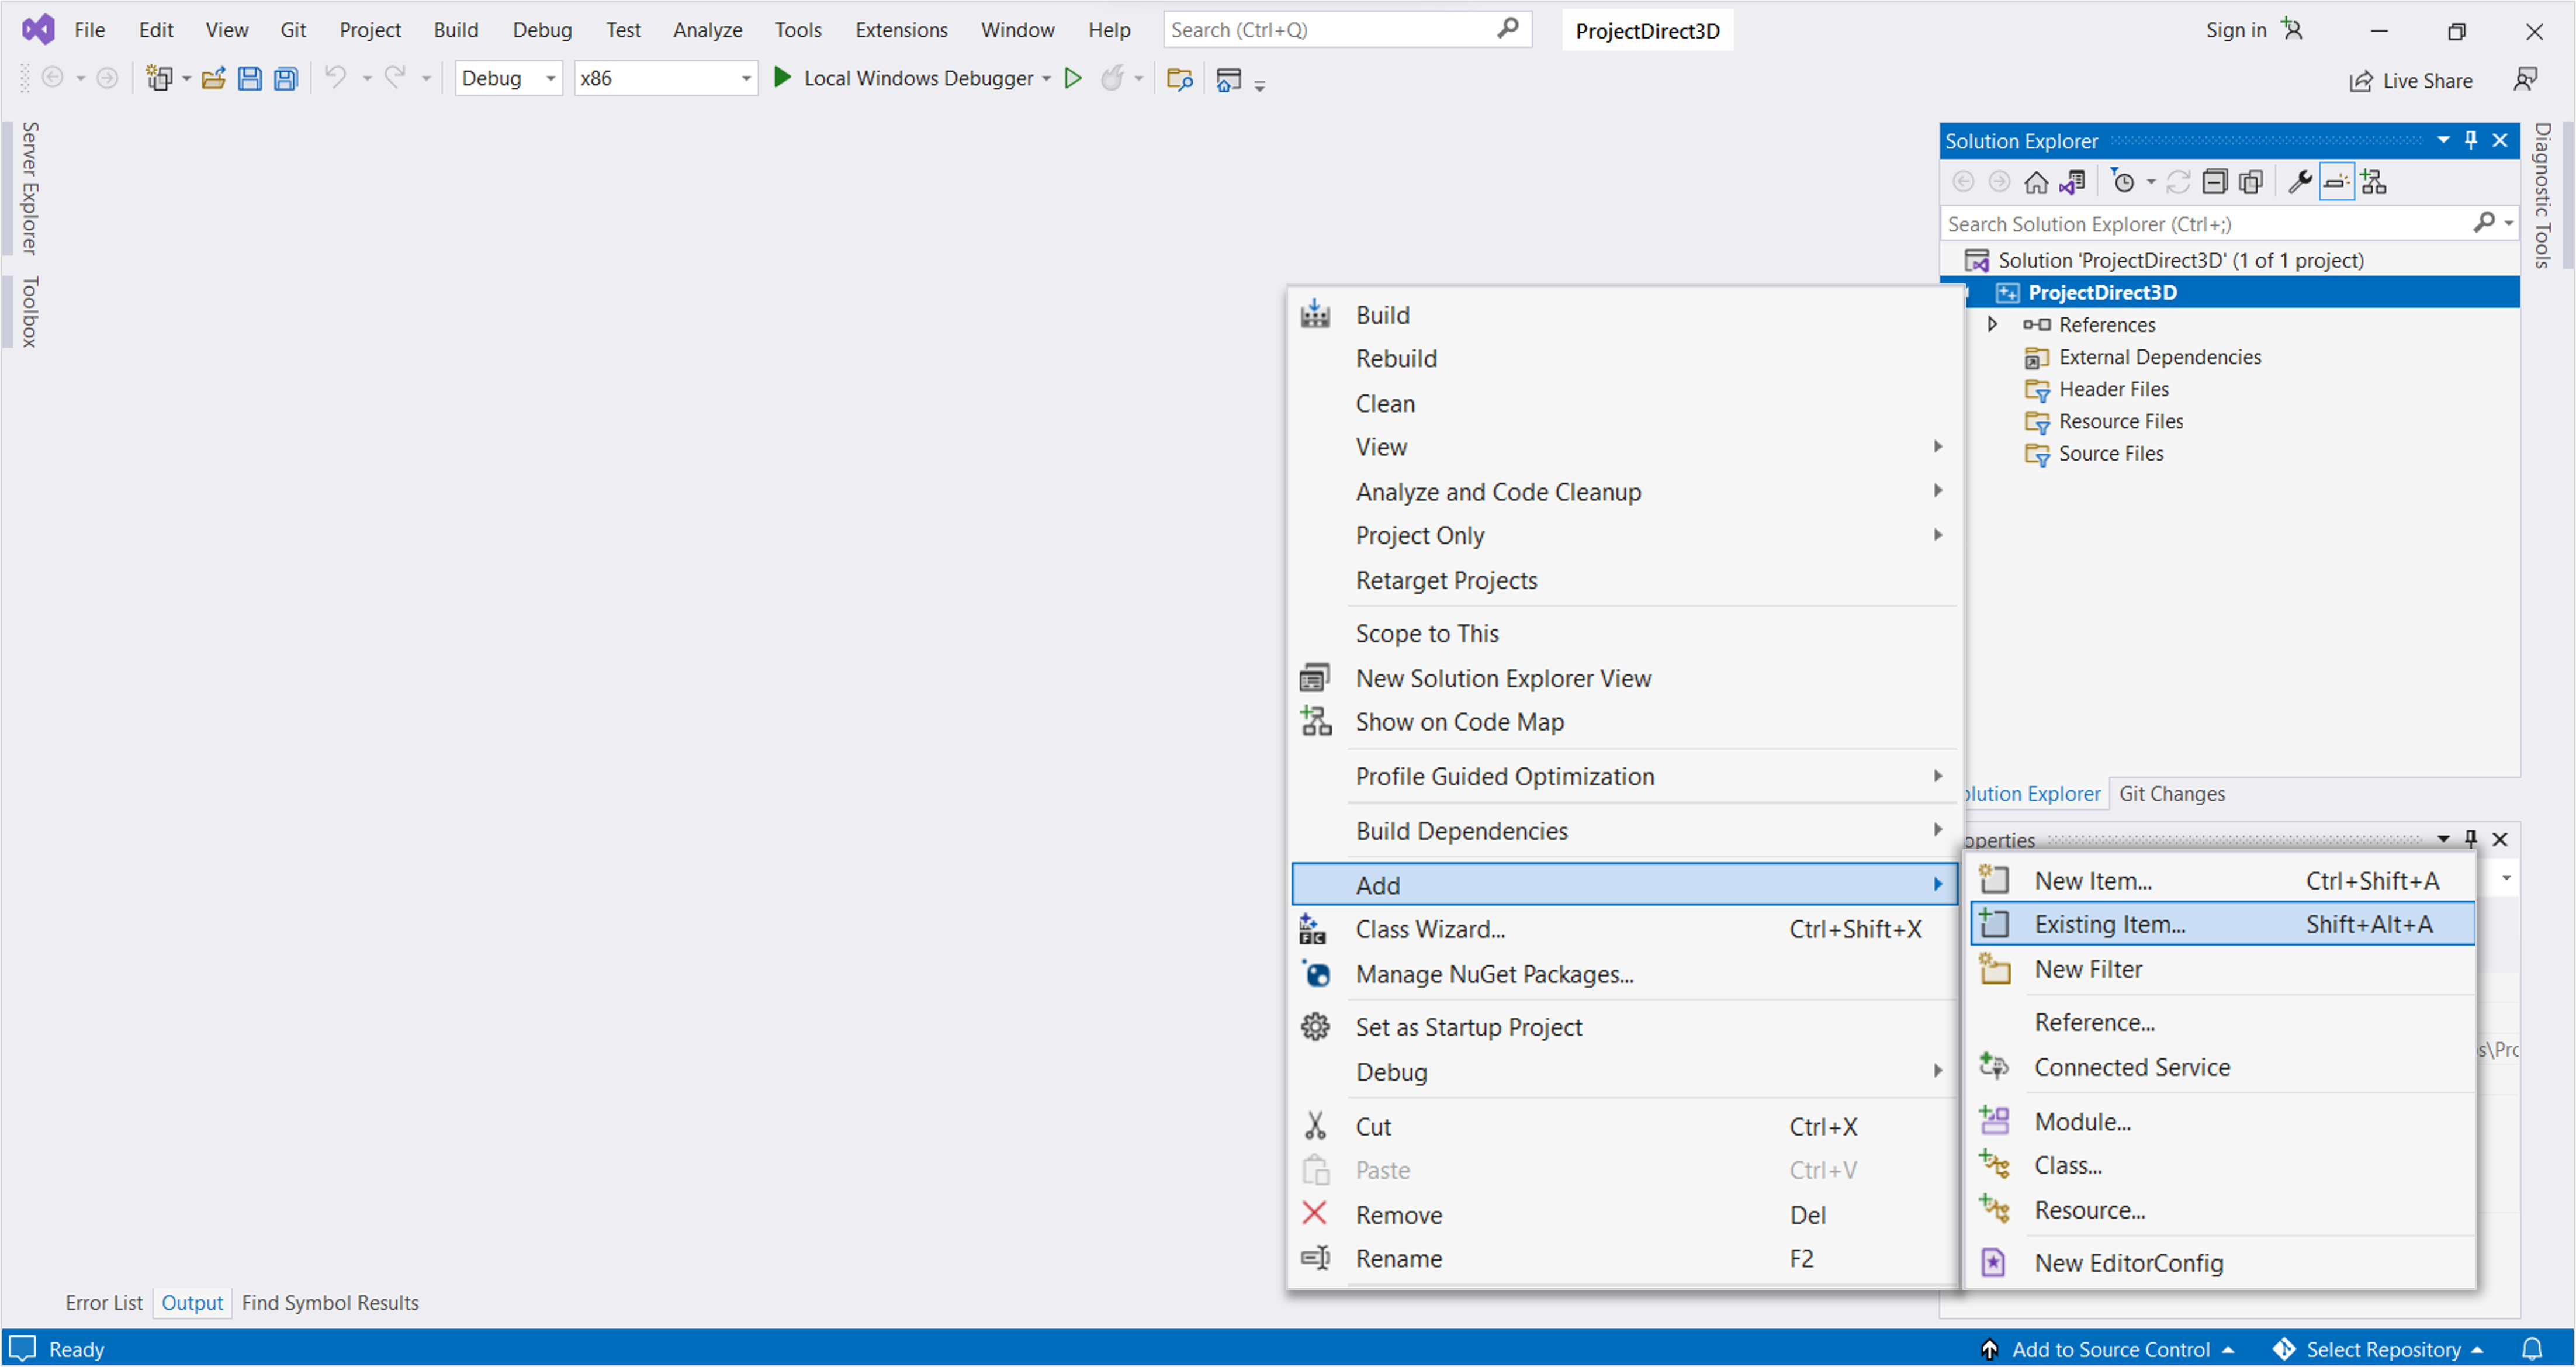
\includegraphics[width=\textwidth]{Images/3/3.Intro.5.9.2}
                    \caption{اضافه کردن فایل به پروژه}
                    \label{fig:3.Intro.5.9.2}
                \end{figure}

                از پنجره ی باز شده به مسیر دایرکتوری \lr{Common} بروید و تمامی فایل ها با پسوند \lr{.h} و \lr{.cpp} را انتخاب کنید  (شکل \ref{fig:3.Intro.5.9.3}).

                \begin{figure}[H]
                    \centering
                    \setlength{\belowcaptionskip}{-10pt}
                    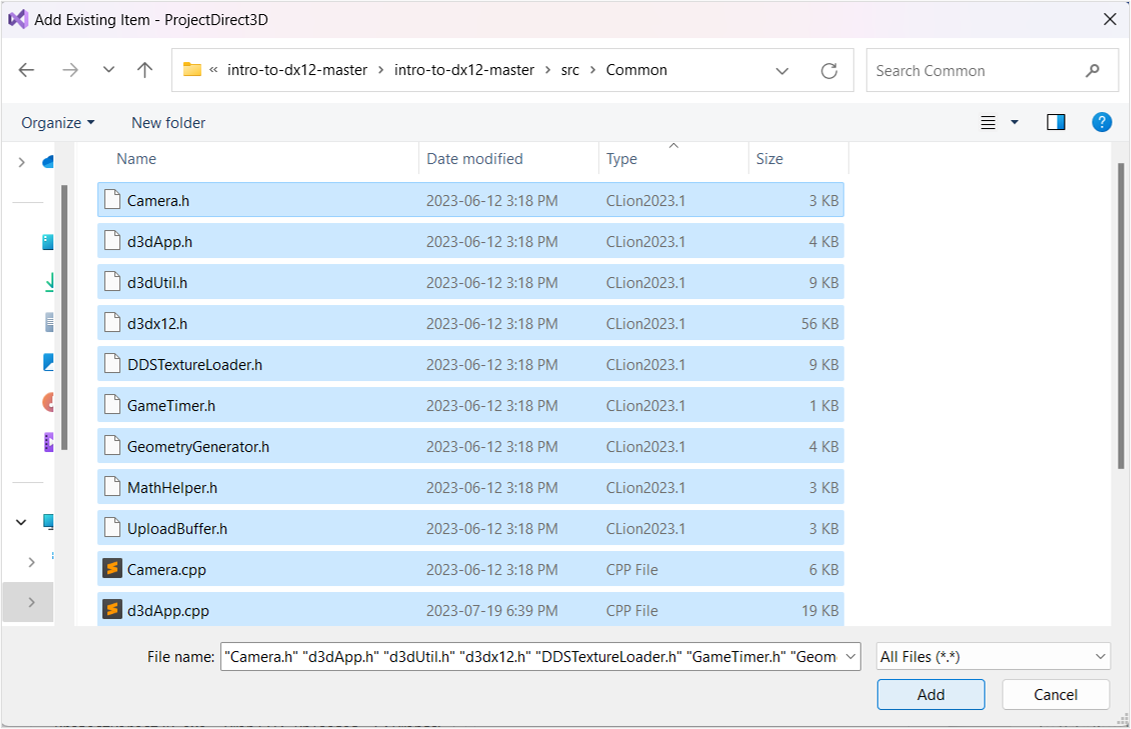
\includegraphics[width=\textwidth]{Images/3/3.Intro.5.9.3}
                    \caption{پنجره ی \lr{Add Exiting Item}}
                    \label{fig:3.Intro.5.9.3}
                \end{figure}

                در انتها باید مانند (شکل \ref{fig:3.Intro.5.9.1} شود).

                \begin{figure}[H]
                    \centering
                    \setlength{\belowcaptionskip}{-10pt}
                    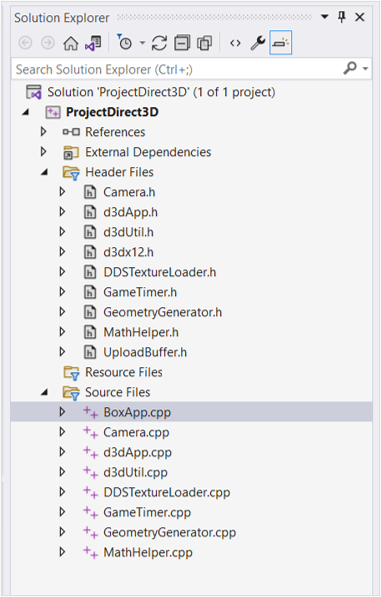
\includegraphics[scale=0.7]{Images/3/3.Intro.5.9.1}
                    \caption{قسمت \lr{Solution Explorer}}
                    \label{fig:3.Intro.5.9.1}
                \end{figure}
            }

            \item {اکنون فایل های کد منبع جزئی از پروژه بوده و میتوانید به منوی اصلی رفته و \lr{Debug->Start Debugging} را انتخاب کنید تا کد آزمایشی کامپایل ، لینک و اجرا شود (شکل \ref{fig:3.Intro.5.10}).}
        \end{enumerate}

        \begin{figure}[H]
            \centering
            \setlength{\belowcaptionskip}{-10pt}
            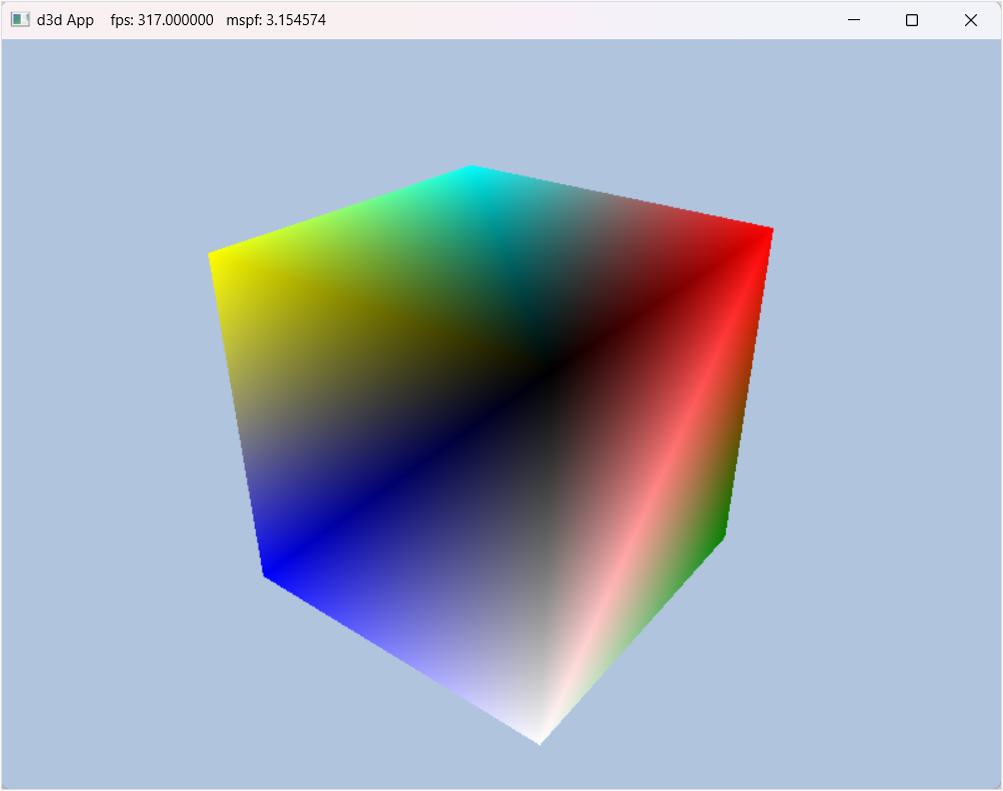
\includegraphics[scale=0.7]{Images/3/3.Intro.5.10}
            \caption{خروجی برنامه}
            \label{fig:3.Intro.5.10}
        \end{figure}
    \end{spacing}
}
\textbf{\vspace{-10pt}}

\begin{theo}{thm:pythagoras}
{
    \Large
    \begin{spacing}{1.5}
        در صورتی که هنگام اجرا با ارور \lr{\enquote*{\&} requires I-value} مواجه شدید (شکل \ref{fig:3.Intro.5.11}) ،
        از پنجره ی \lr{Property} ، \lr{C/C++->Language}  را انتخاب کنید و از قسمت \lr{Conformance mode} را روی \lr{No (/permissive)} بگذارید (شکل \ref{fig:3.Intro.5.12})

        \begin{figure}[H]
            \centering
            \setlength{\belowcaptionskip}{-10pt}
            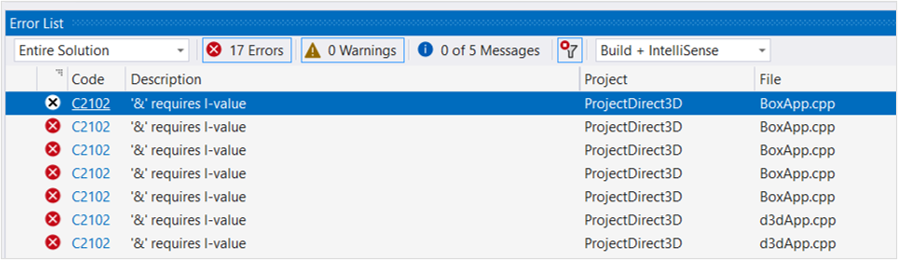
\includegraphics[width=\textwidth]{Images/3/3.Intro.5.11}
            \caption{ارور \lr{\enquote*{\&} requires I-value}}
            \label{fig:3.Intro.5.11}
        \end{figure}

        \begin{figure}[H]
            \centering
            \setlength{\belowcaptionskip}{-10pt}
            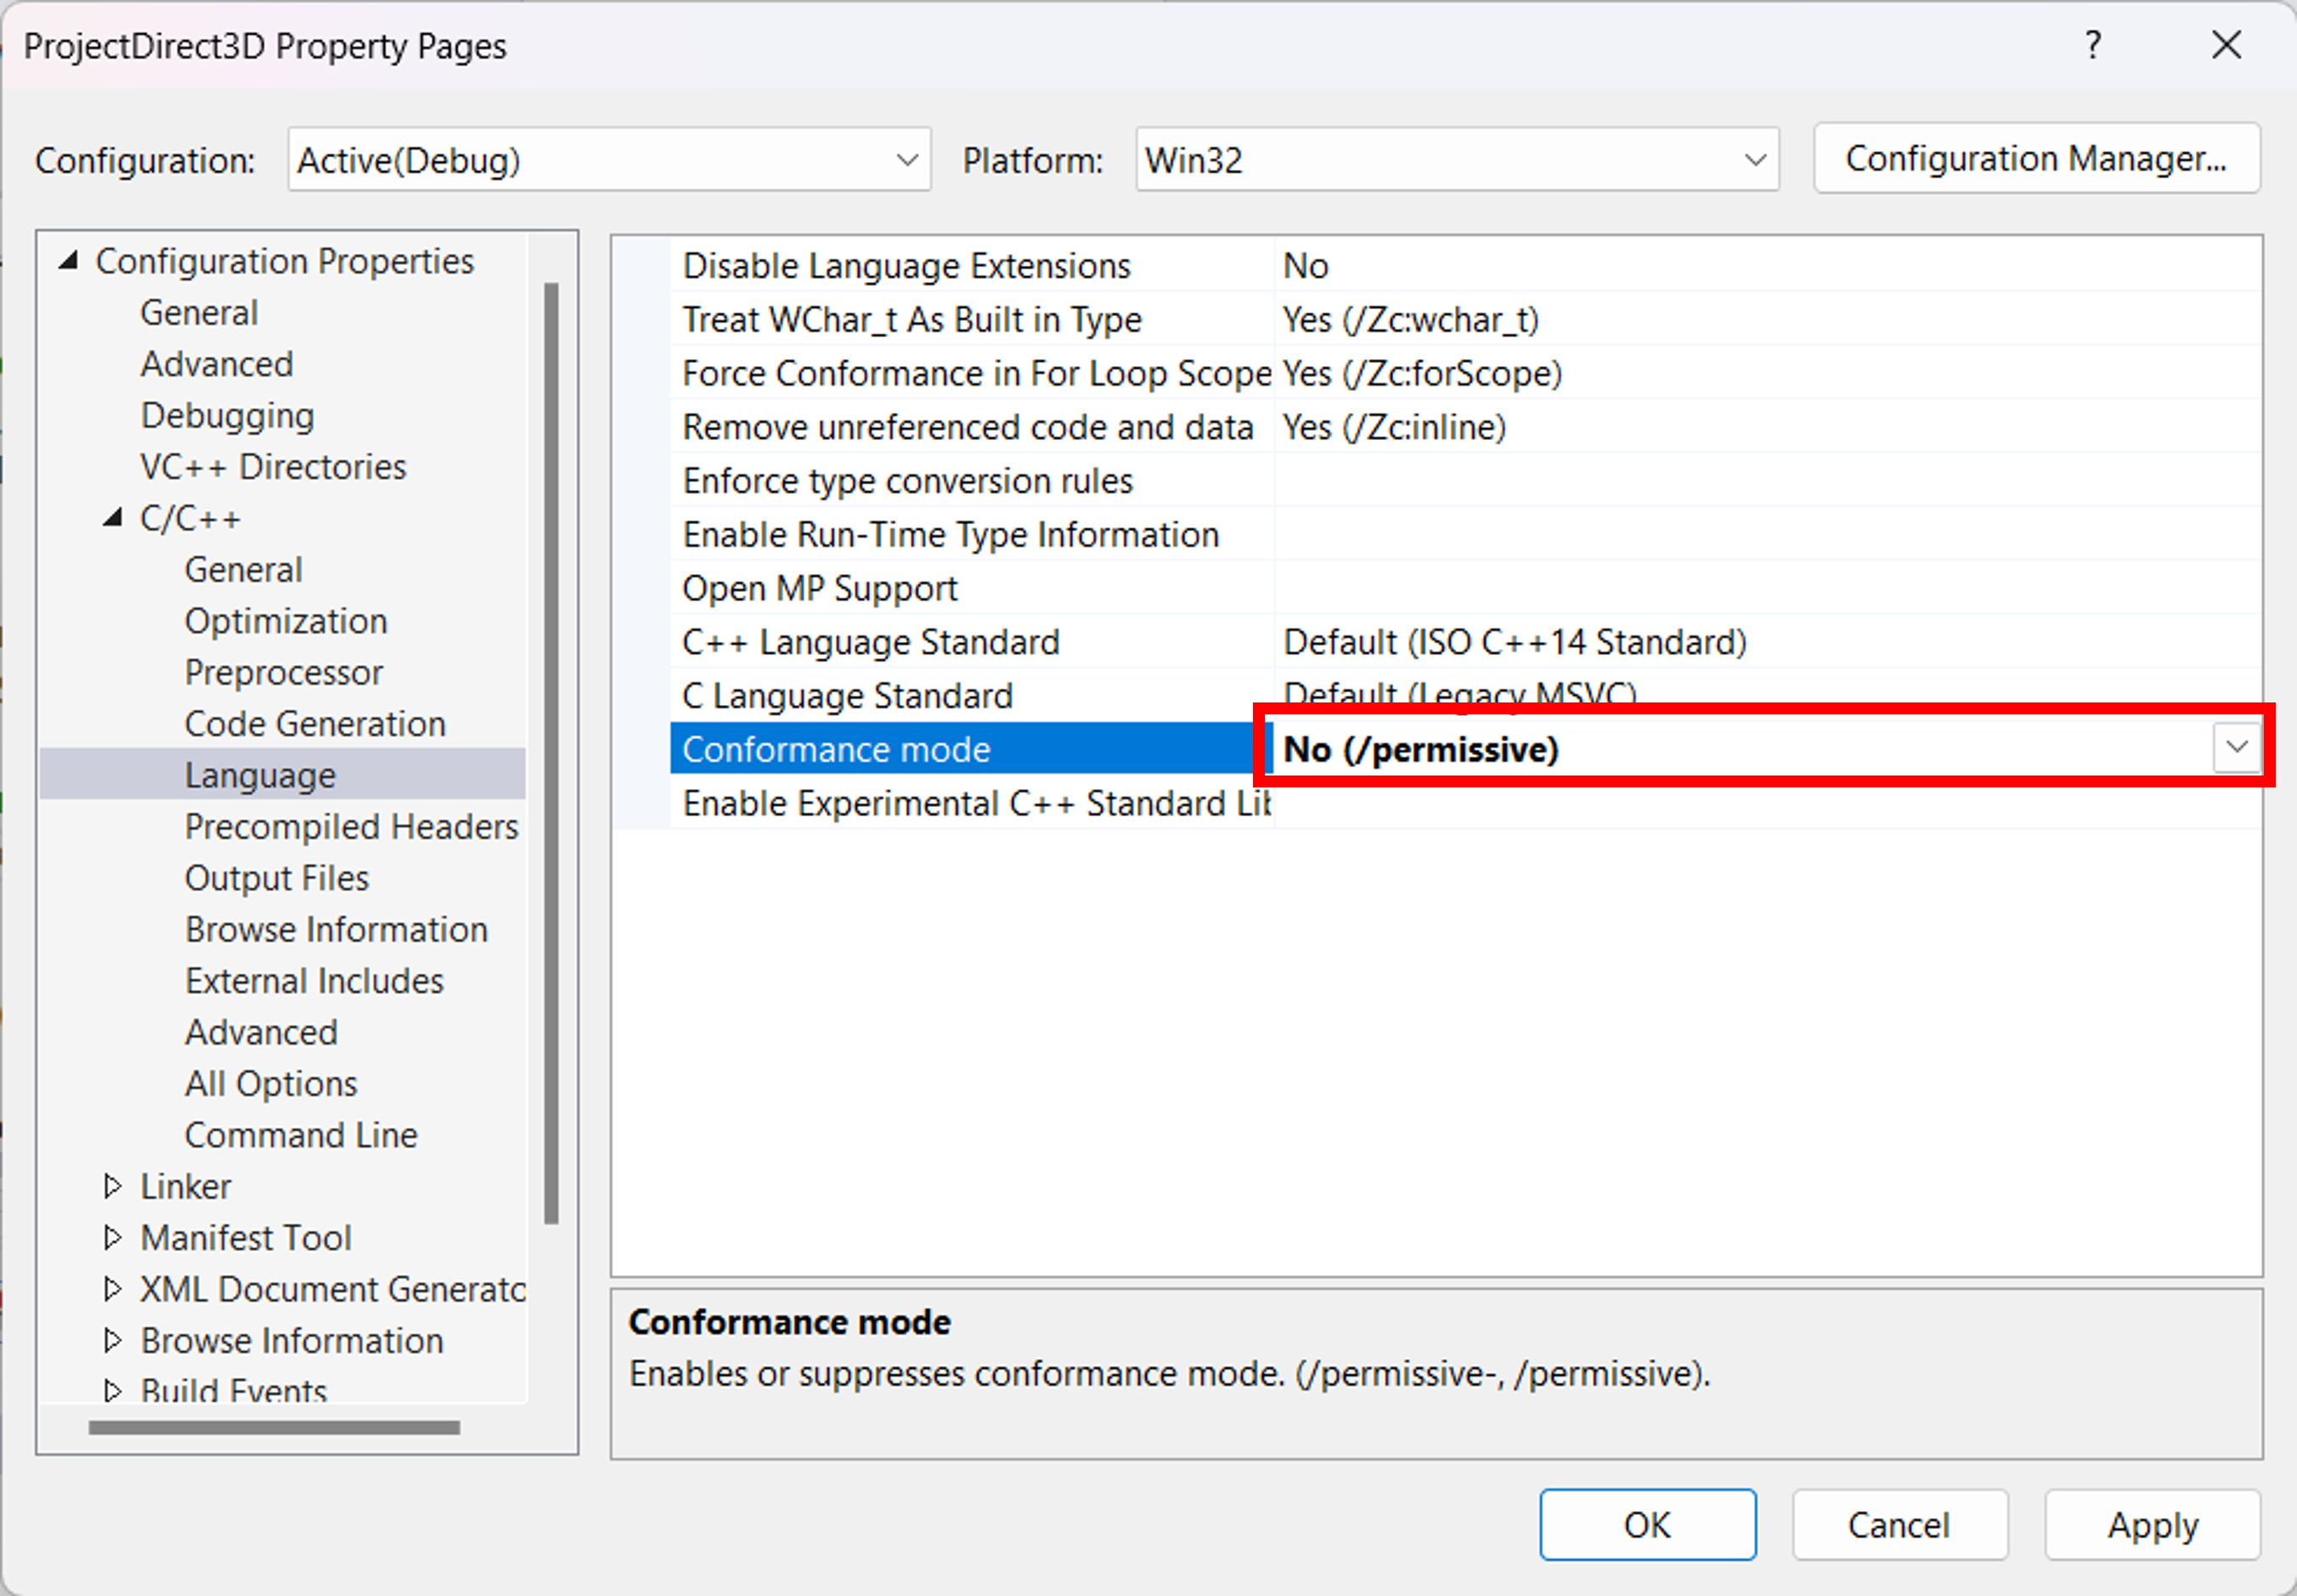
\includegraphics[width=\textwidth]{Images/3/3.Intro.5.12}
            \caption{تنظیمات \lr{C/C++->Language}}
            \label{fig:3.Intro.5.12}
        \end{figure}

        در صورتی که ارور رفع نشد ، از قسمت بالا (شکل \ref{fig:3.Intro.5.13}) ، \lr{x86} را انتخاب کنید.

        \begin{figure}[H]
            \centering
            \setlength{\belowcaptionskip}{-10pt}
            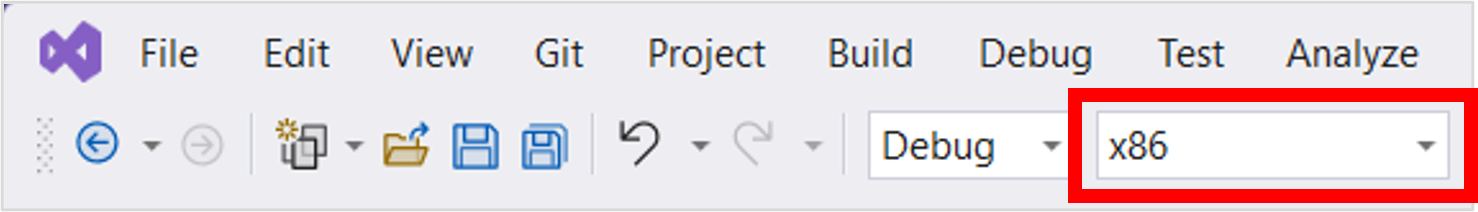
\includegraphics[width=\textwidth]{Images/3/3.Intro.5.13}
            \caption{نحوه ی اجرا به صورت \lr{x86} \textbf{\vspace{12pt}}}
            \label{fig:3.Intro.5.13}
        \end{figure}
    \end{spacing}
}
\end{theo}
\textbf{\vspace{6pt}}

%-----------------------------------------------------------------------------------------------------------%
\newpage

%% ----- Sessions ----- %
    \pagenumbering{arabic}
    %-----------------------------------------------------------------------------------------------------------%
\newpage

\part{پیشنیاز های ریاضی}
{
    \Large
    \begin{spacing}{1.5}
        بازی های ویدیویی سعی در شبیه سازی دنیای مجازی دارند.
        با این حال، کامپیوترها، به دلیل ماهیت خود، اعداد را محاسبه می کنند. بنابراین مشکل چگونگی انتقال یک جهان به یک کامپیوتر مطرح می شود.
        پاسخ این مشکل میتواند اینگونه باشد که جهان‌های ما و فعل و انفعالات موجود در آن را کاملاً ریاضی توصیف کنیم.
        در نتیجه، ریاضیات نقش اساسی در توسعه بازی های ویدیویی ایفا می کند.

        در این بخش، ابزارهای ریاضی که در این کتاب مورد استفاده قرار گرفته اند، معرفی می کنیم. تأکید ما بر بردارها، سیستم های مختصات، ماتریس ها و تبدیل ها است، زیرا این ابزارها تقریباً در همه ی برنامه های نمونه این کتاب استفاده شده اند.
        علاوه بر توضیحات ریاضی، بررسی و نمایش کلاس ها و توابع مربوطه از کتابخانه ریاضی DirectX را نیز ارائه میکنیم.

        توجه داشته باشید که موضوعاتی که در اینجا مورد بررسی قرار می‌گیرند، تنها مواردی هستند که برای درک ادامه ی این کتاب ضروری اند.
        این کتاب به هیچ وجه راه حل جامعی برای ریاضیات بازی های ویدیویی نیست.

        \textbf{\vspace{20pt}}
        \begin{theo}{thm:pythagoras}
            \Large
            برای خوانندگانی که مایل به ارجاع کامل تر به ریاضیات بازی های ویدیویی هستند، کتاب های زیر را توصیه می کنیم.
            \lr{
                \begin{enumerate}
                    \item {Essential Mathematics for Games and Interactive Applications: A Programmer's Guide (Verth04)}
                    \item {Mathematics for 3D Game Programming and Computer Graphics (Lengyel02)}
                \end{enumerate}
            }
        \end{theo}
        \textbf{\vspace{40pt}}

        \textbf{فصل 1، جبر برداری:} بردارها اساسی ترین اشیاء ریاضی مورد استفاده در بازی های کامپیوتری هستند.
        ما از بردارها برای نشان دادن موقعیت ها، جابجایی ها، جهت ها، سرعت ها و نیروها استفاده می کنیم.
        در این فصل، بردارها و عملیات مورد استفاده برای کار با آنها را مطالعه می کنیم.

        \textbf{فصل 2، جبر ماتریسی:} ماتریس ها روشی کارآمد و فشرده برای نمایش تبدیل ها ارائه می دهند.
        در این فصل با ماتریس ها و عملیات تعریف شده بر روی آنها آشنا می شویم.

        \textbf{فصل 3، تبدیل:} این فصل سه تبدیل هندسی اساسی را بررسی می کند: مقیاس بندی، چرخش و انتقال.
        ما از این تبدیل ها برای کار با اشیاء سه بعدی در فضا استفاده می کنیم.
        علاوه بر این، تغییر تبدیل مختصات را توضیح می دهیم، که برای تبدیل مختصات هندسی از یک سیستم مختصات به سیستم دیگر استفاده می شود.
    \end{spacing}
}

\setcounter{chapter}{1}

\textbf{\vspace{80pt}}
\chapter{\textbf{جبر برداری}}
\textbf{\vspace{70pt}}
{
    \Large
    \begin{spacing}{1.5}
        بردارها نقش مهمی در گرافیک کامپیوتری، تشخیص برخورد و شبیه سازی فیزیکی ایفا می کنند که همگی اجزای رایج در بازی های ویدئویی مدرن هستند.
        رویکرد ما در اینجا غیر تخصصی و عملی است به همین دلیل پیشنهاد ما کتاب \lr{Verth04} (در نکته ی قبل ذکر شده است) است که کتابی اختصاصی برای ریاضیات بازی های سه بعدی/گرافیک است.
        ما بر اهمیت بردارها بسیار تأکید داریم زیرا در بیشتر برنامه های آزمایشی این کتاب استفاده شده اند.

        \textbf{\vspace{20pt}}
        \textbf{\hspace{-40pt}\LARGE اهداف:}

        \begin{enumerate}
            \item {یادگیری نحوه نمایش بردارها به صورت هندسی و عددی}
            \item {یادگیری عملیات تعریف شده بر روی بردارها و کاربردهای هندسی آنها}
            \item {آشنایی با توابع برداری و کلاس های کتابخانه \lr{DirectXMath}}
        \end{enumerate}
    \end{spacing}
}
%-----------------------------------------------------------------------------------------------------------%
\newpage

\section{
    \huge
    \textbf{بردار ها}
}
{
    \Large
    \begin{spacing}{1.4}
        بردار به کمیتی اشاره دارد که هم اندازه و هم جهت دارد.
        به کمیت هایی که اندازه و جهت دارند، کمیت های برداری گویند.
        نمونه‌هایی از کمیت‌های برداری عبارتند از نیروها (نیرو در جهت خاصی با قدرت/اندازه معین اعمال می‌شود)، جابه‌جایی (جهت برآیند و فاصله حرکت ذره)، و سرعت‌ها (سرعت و جهت).
        بنابراین، بردارها برای نمایش نیروها، جابجایی ها و سرعت ها استفاده می شوند.
        به علاوه، ما از بردارها برای تعیین جهات خالص استفاده می کنیم،
        مانند جهتی که بازیکن در یک بازی سه بعدی به آن نگاه میکند،
        جهتی که یک چند ضلعی رو به آن قرار دارد، جهتی که پرتوی نور در آن حرکت می کند،
        یا جهتی که در آن یک پرتو نور از یک سطح منعکس می شود.

        اولین مرحله در توصیف ریاضی بردار ، توصیف هندسی آن است: ما به صورت گرافیکی یک بردار را با یک پاره خط جهت دار مشخص می کنیم (شکل \ref{fig:4.Session.1.1.1})، که در آن طول نشان دهنده بزرگی بردار و سر کمان نشان دهنده جهت بردار است.
        به این نکته باید توجه کنید که مکانی که در آن یک بردار رسم می‌کنیم بی‌اهمیت است، زیرا تغییر مکان، بزرگی یا جهت را تغییر نمی‌دهد (دو ویژگی ای که بردار دارد).
        بنابراین می گوییم دو بردار برابر هستند اگر و تنها اگر طول یکسانی داشته و در یک جهت باشند.
        بنابراین، بردارهای \lr{u} و \lr{v} ترسیم شده در قسمت آ شکل \ref{fig:4.Session.1.1.1} در واقع برابر اند زیرا طول و جهت یکسانی دارند.
        در واقع، چون مکان برای بردارها اهمیتی ندارد، ما می‌توانیم یک بردار را بدون تغییر هویت آن ، انتقال دهیم (زیرا انتقال نه طول و نه جهت را تغییر می‌دهد).
        توجه داشته باشید که ما می‌توانیم \lr{u} را طوری انتقال دهیم که کاملاً بر \lr{v} همپوشانی داشته باشد (و بالعکس) و در نتیجه آنها را غیرقابل تشخیص کنیم. این نیز دلیلی برای برابری آنهاست.

        \begin{figure}[H]
            \centering
            \setlength{\belowcaptionskip}{-10pt}
            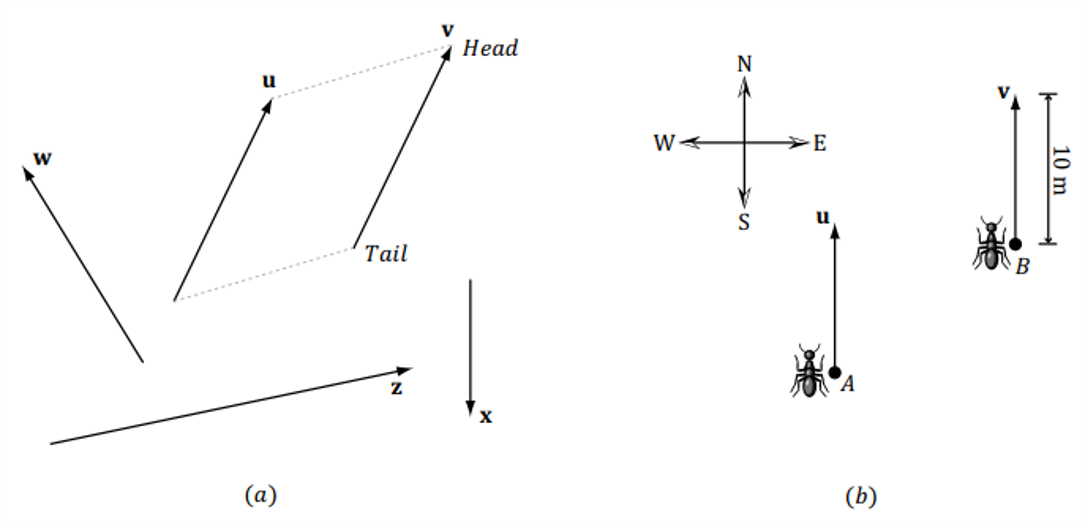
\includegraphics[width=0.85\textwidth]{Images/4/4.Session.1.1.1}
            \caption{(الف) بردار هایی که روی صفحه ی دوبعدی کشیده شده اند.
                (ب) بردار هایی که مورچه ها را برای حرکت 10 متر در جهت شمال راهنمایی میکنند.}
            \label{fig:4.Session.1.1.1}
        \end{figure}

        به عنوان یک مثال فیزیکی، بردارهای \lr{u} و \lr{v} در قسمت ب شکل \ref{fig:4.Session.1.1.1} هر دو به مورچه ها میگویند در دو نقطه مختلف \lr{A} و \lr{B} ده متر به سمت شمال حرکت کنند.
        دوباره \lr{u = v} را داریم.
        بردارها خود مستقل از موقعیت هستند و
        آنها به سادگی به مورچه ها آموزش می دهند که چگونه از جایی که هستند، ده متر (طول) به سمت شمال (جهت) حرکت کنند.

    \end{spacing}
}

\subsection{\textbf{\LARGE بردارها و سیستم های مختصات}}
{
    \Large
    \begin{spacing}{1.5}
        اکنون می‌توانیم عملیات هندسی مفیدی را روی بردارها تعریف کنیم، که سپس می‌توان از آنها برای حل مسائل مربوط به کمیت‌های برداری استفاده کرد.
        با این حال، از آنجایی که کامپیوتر نمی تواند با بردارها به صورت هندسی کار کند، باید راهی برای تعیین عددی بردارها پیدا کنیم.
        بنابراین یک سیستم مختصات سه بعدی را در فضا معرفی می کنیم و همه بردارها را طوری انتقال میدهیم که دم آن ها با مبدا منطبق باشد (شکل \ref{fig:4.Session.1.1.2}).

        \begin{figure}[H]
            \centering
            \setlength{\belowcaptionskip}{-10pt}
            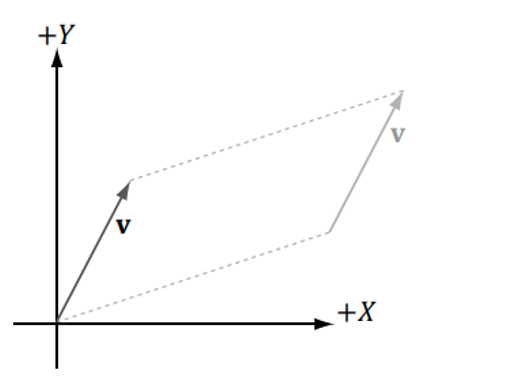
\includegraphics[width=0.48\textwidth]{Images/4/4.Session.1.1.2}
            \caption{\lr{v} را طوری انتقال میدهیم که دم آن با مبدأ سیستم مختصات منطبق
            باشد. وقتی دم یک بردار با مبدا منطبق می شود، می گوییم که در موقعیت استاندارد قرار دارد.}
            \label{fig:4.Session.1.1.2}
        \end{figure}

        سپس می‌توانیم یک بردار را با تعیین مختصات سر آن شناسایی کنیم و مانند شکل \ref{fig:4.Session.1.1.3}، \lr{v = (x, y, z)} را بنویسیم.
        اکنون می توانیم یک بردار را با سه \lr{float} در یک برنامه کامپیوتری نشان دهیم.

        \begin{theo}{thm:pythagoras}
            \Large
            اگر به صورت دو بعدی کار کنیم، فقط از یک سیستم مختصات دو بعدی استفاده می کنیم و بردار فقط دو مختصات دارد:
            \lr{v = (x, y)} و می توانیم یک بردار را با دو \lr{float} در یک برنامه کامپیوتری نشان دهیم.
        \end{theo}

        \begin{figure}[H]
            \centering
            \setlength{\belowcaptionskip}{-10pt}
            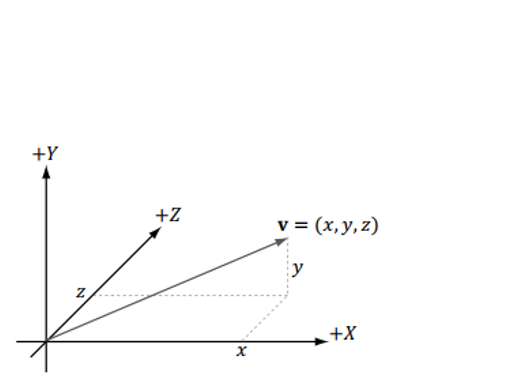
\includegraphics[width=0.48\textwidth]{Images/4/4.Session.1.1.3}
            \caption{یک بردار مشخص شده توسط مختصات نسبت به یک سیستم مختصات.}
            \label{fig:4.Session.1.1.3}
        \end{figure}

        شکل \ref{fig:4.Session.1.1.4} را در نظر بگیرید که یک بردار \lr{v} و دو فریم (\lr{frame}) در فضا را نشان می دهد. (توجه داشته باشید که ما از اصطلاحات فریم، فریم مرجع، فضا و سیستم مختصات استفاده می کنیم که همگی در این کتاب به یک معنا هستند.)
        می توانیم \lr{v} را طوری انتقال دهیم که در هر یک از دو سیستم مختصات در موقعیت استاندارد قرار گیرد. با این حال، مشاهده کنید که مختصات بردار \lr{v} نسبت به سیستم مختصات \lr{A} با مختصات بردار \lr{v} نسبت به سیستم مختصات \lr{B} متفاوت است.
        به عبارت دیگر، همان بردار \lr{v} نمایش مختصاتی متفاوتی برای سیستم مختصات های متمایز دارد.

        \begin{figure}[H]
            \centering
            \setlength{\belowcaptionskip}{-10pt}
            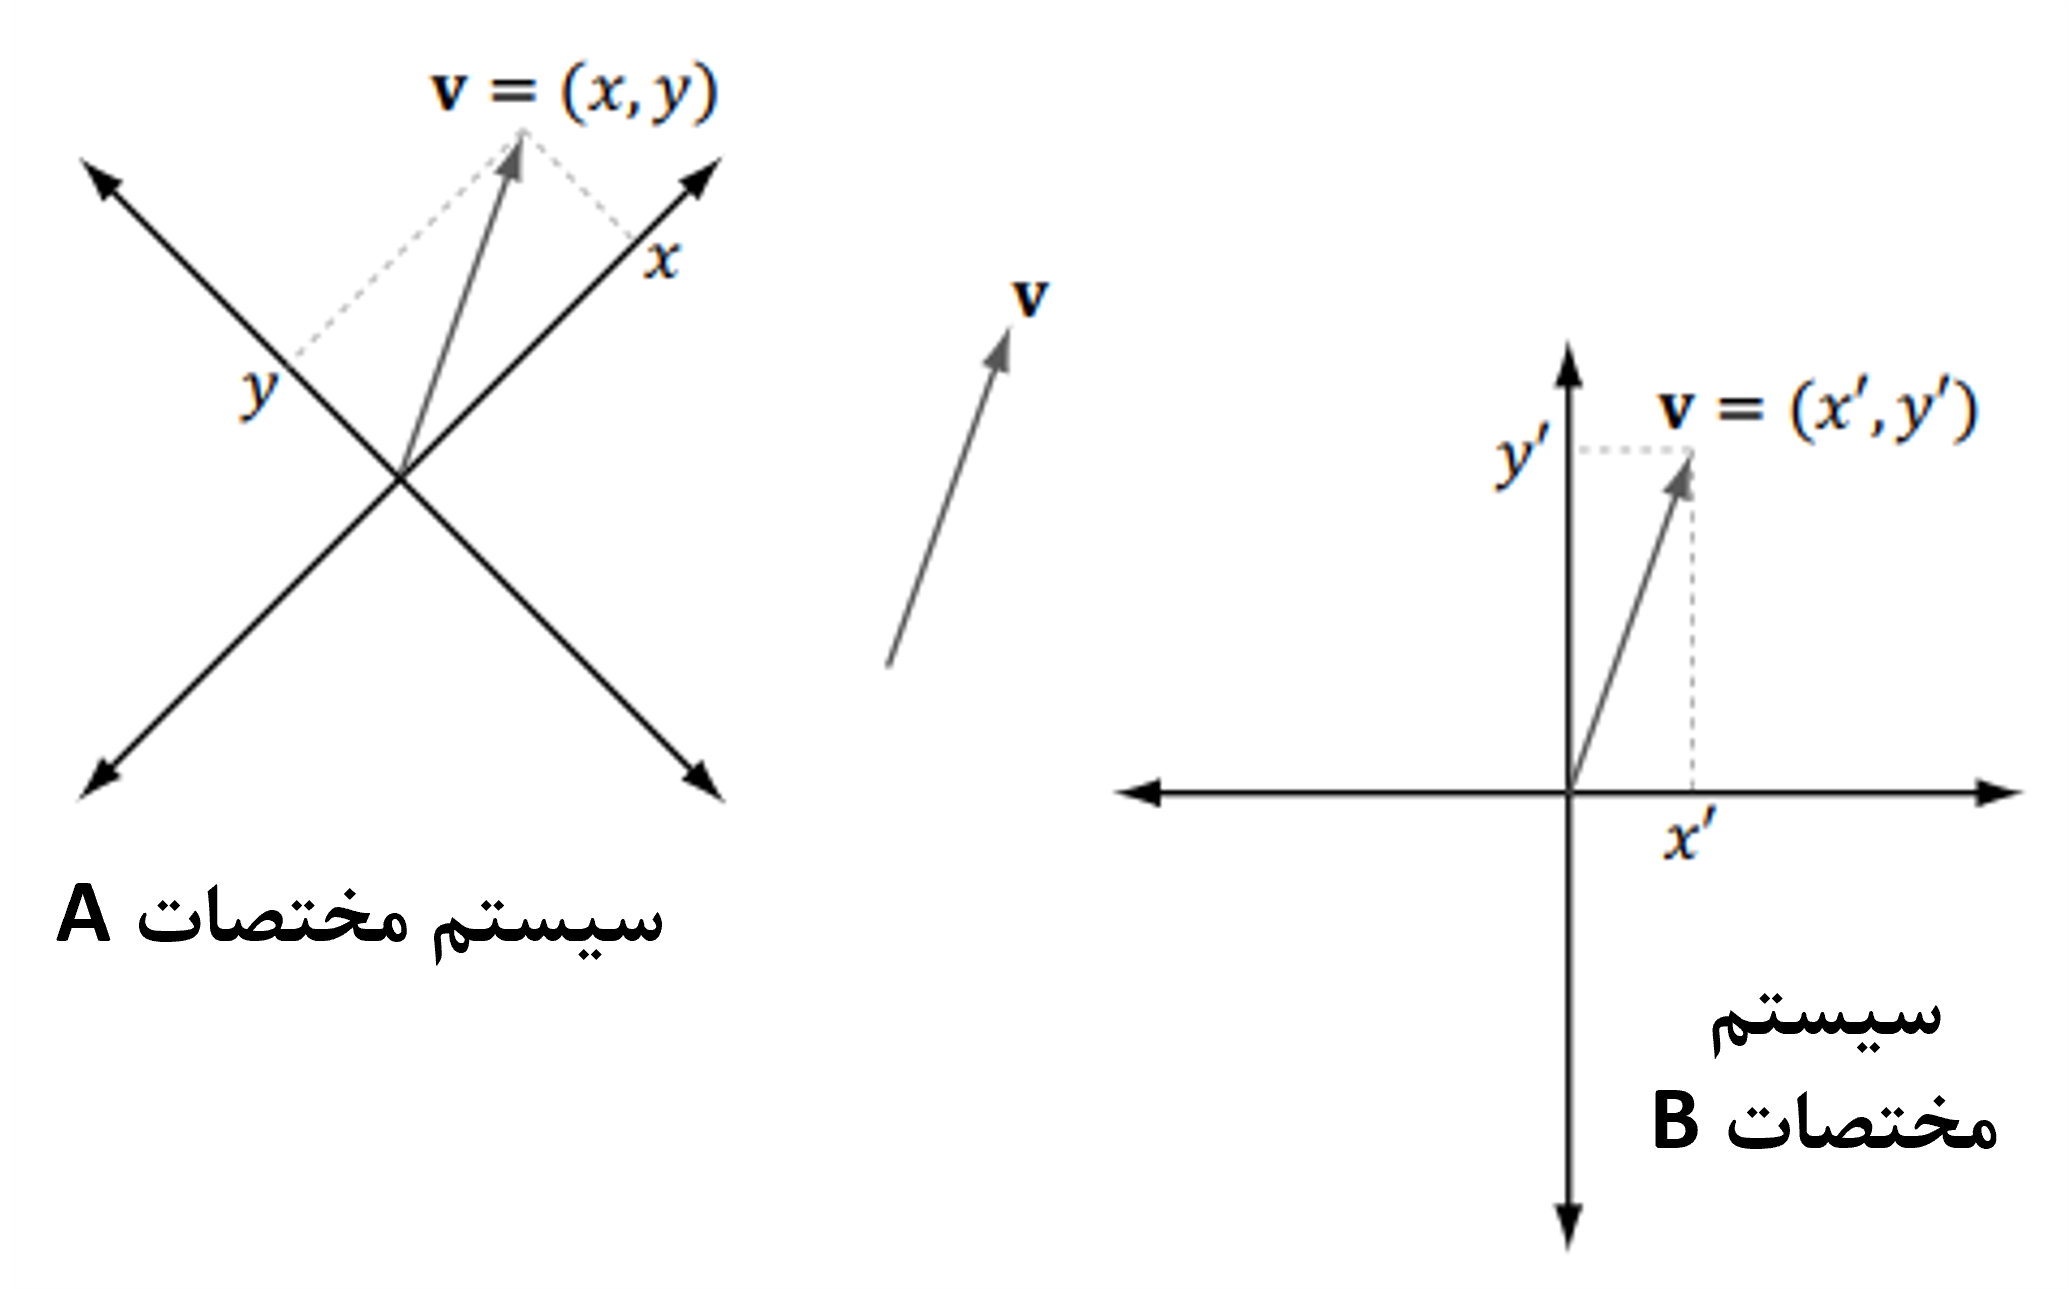
\includegraphics[width=0.8\textwidth]{Images/4/4.Session.1.1.4}
            \caption{همان بردار v زمانی که نسبت به سیستم مختصات های مختلف تعریف شود، مختصات متفاوتی دارد.}
            \label{fig:4.Session.1.1.4}
        \end{figure}

        این ایده شبیه به مثال دما است. آب در 100 درجه سانتیگراد یا 212 درجه فارنهایت می جوشد.
        دمای فیزیکی آب جوش بدون توجه به مقیاس یکسان است (یعنی نمی‌توانیم نقطه جوش را با انتخاب مقیاس متفاوت کاهش دهیم)،
        اما بر اساس مقیاسی که استفاده می‌کنیم عدد اسکالر متفاوتی را به دما اختصاص می‌دهیم.
        به طور مشابه، برای یک بردار، جهت و بزرگی آن، که در پاره خط جهت دار تعبیه شده است، تغییر نمی کند.
        فقط مختصات آن بر اساس سیستم مختصات که برای توصیف آن استفاده می کنیم تغییر می کند.
        این نکته ی مهمی ست زیرا به این معنی است که هرگاه یک بردار را با مختصات شناسایی کنیم، آن مختصات نسبت به برخی از سیستم های مختصات هستند.
        اغلب در گرافیک های کامپیوتری سه بعدی، از بیش از یک سیستم مختصات استفاده می کنیم و بنابراین، باید شناسایی کنیم که مختصات یک بردار نسبت به کدام سیستم مختصات است.
        علاوه بر این، ما باید بدانیم که چگونه مختصات برداری را از یک سیستم مختصات به سیستم مختصات دیگر تبدیل کنیم.
        \textbf{\vspace{-10pt}}
        \begin{theo}{thm:pythagoras}
            \Large
            مشاهده میکنیم که بردارها و نقاط را می توان با مختصات (\lr{x, y, z}) نسبت به یک سیستم مختصات توصیف کرد.
            با این حال، بردارها و نقاط یکسان نیستند؛ یک نقطه نشان دهنده یک مکان در 3 فاصله است، در حالی که یک بردار نشان دهنده یک اندازه و جهت است.
        \end{theo}
        \textbf{\vspace{-50pt}}
    \end{spacing}

    \begin{figure}[H]
        \centering
        \setlength{\belowcaptionskip}{-10pt}
        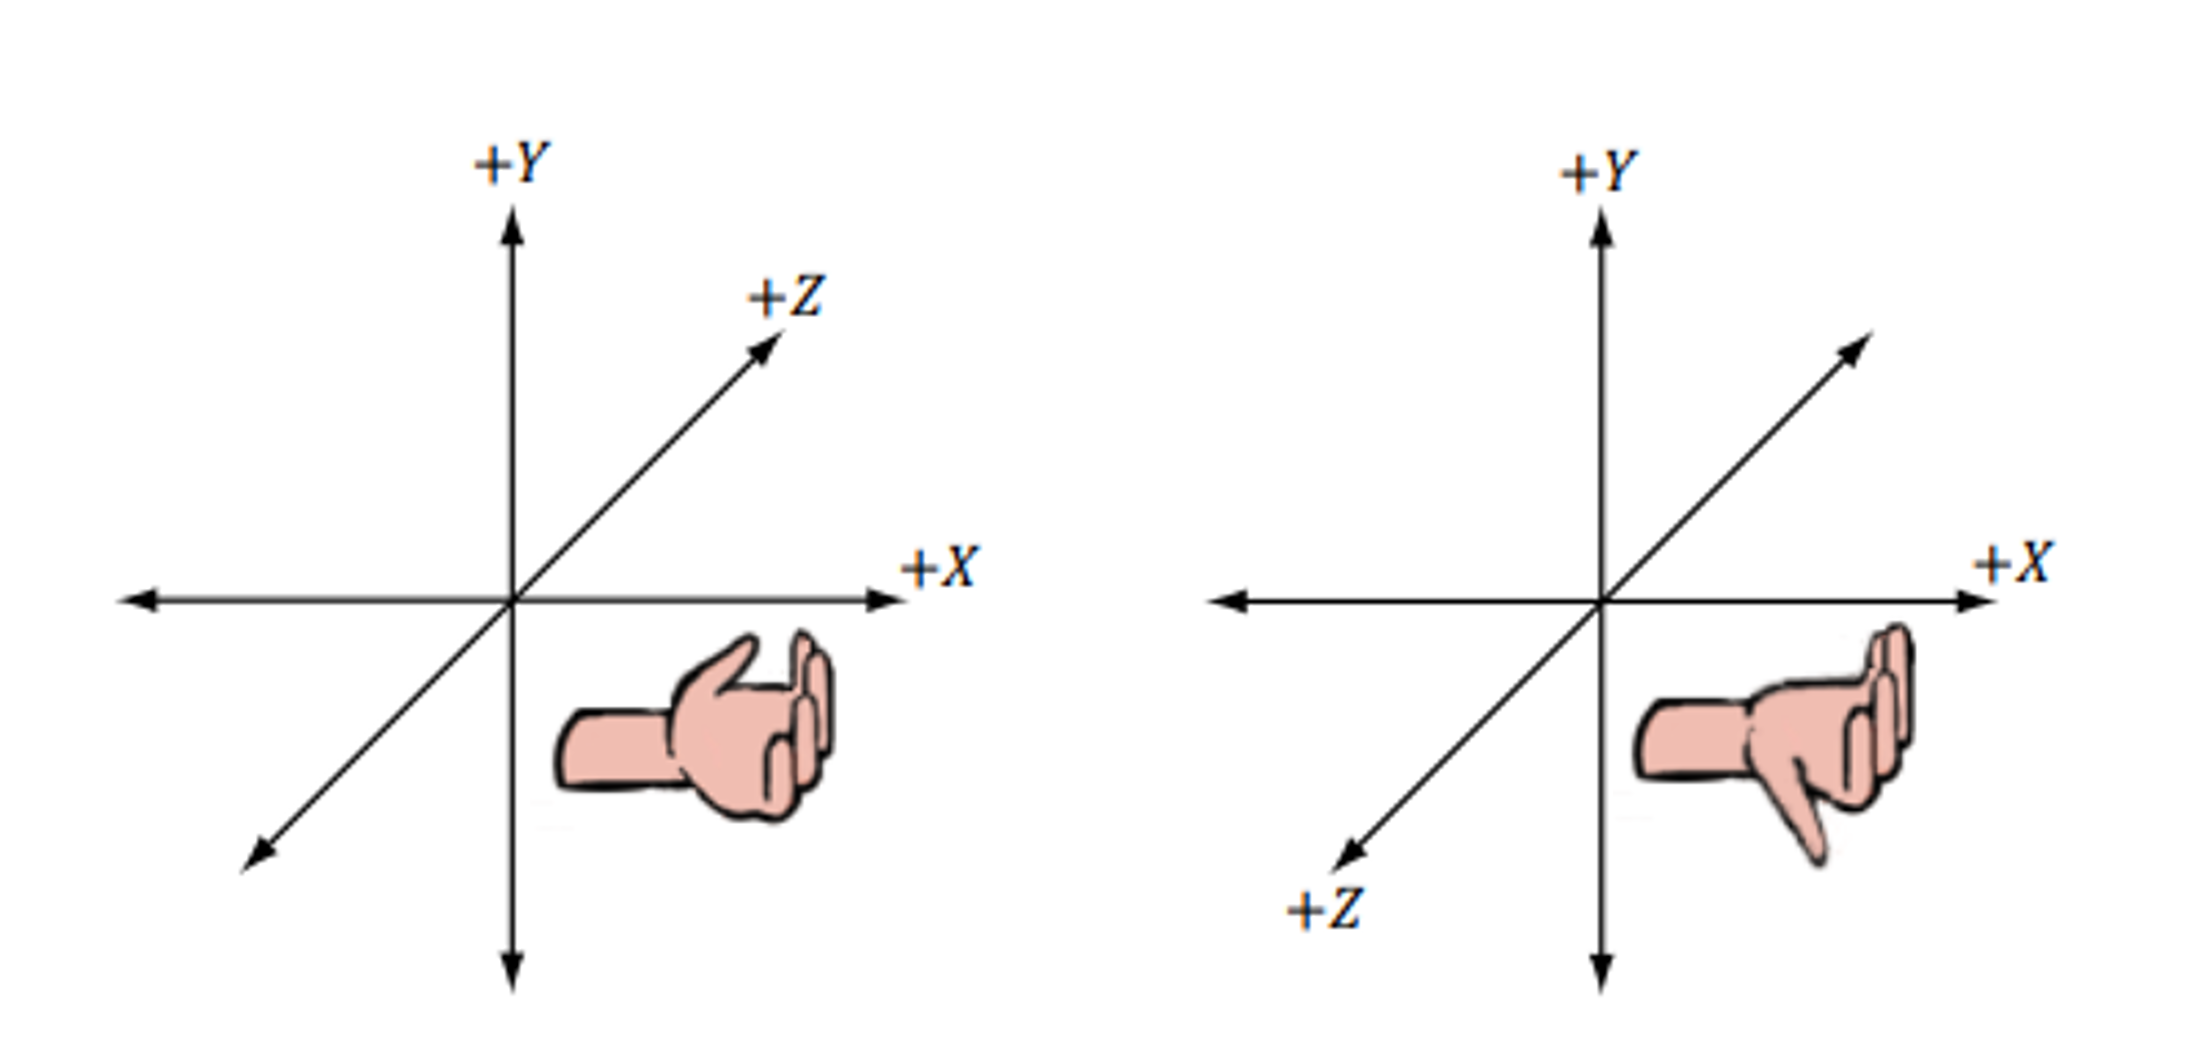
\includegraphics[width=0.9\textwidth]{Images/4/4.Session.1.1.5}
        \caption{در سمت چپ ما یک سیستم مختصات چپگرد داریم که محور z مثبت وارد صفحه می شود. در سمت راست ما یک سیستم مختصات راستگرد داریم که محور z مثبت از صفحه خارج می شود.}
        \label{fig:4.Session.1.1.5}
    \end{figure}
}

\subsection{\textbf{\LARGE سیستم های مختصات چپگرد در مقابل راستگرد}}
{
    \Large
    \begin{spacing}{1.5}
        \lr{Direct3D} از یک سیستم مختصات چپگرد استفاده می کند.
        اگر دست چپ خود را به صورتی بگیرید که انگشتان خود را به سمت محور x مثبت گرفته و سپس انگشتان خود را به سمت محور y مثبت خم کنید، انگشت شست شما در جهت محور z مثبت قرار می گیرد.
        شکل \ref{fig:4.Session.1.1.5} تفاوت بین یک سیستم مختصات چپ دست و راست دست را نشان می دهد.
        توجه کنید که در سیستم مختصات راستگرد، اگر دست راست خود را به صورتی بگیرید که انگشتان خود را به سمت محور x مثبت گرفته و سپس انگشتان خود را به سمت محور y مثبت خم کنید، انگشت شست شما در جهت محور z مثبت اشاره می کند.

    \end{spacing}
}

\subsection{\textbf{\LARGE عملیات بردار پایه}}
{
    \Large
    \begin{spacing}{1.5}
        اکنون با استفاده از نمایش مختصاتی، تساوی، جمع، ضرب اسکالر و تفریق را بر روی بردارها تعریف می کنیم.
        برای این چهار تعریف، فرض میکنیم $\textbf{u}=(u_{x},u_{y},u_{z})$ و  $\textbf{v}=(v_{x},v_{y},v_{z})$.

        \begin{enumerate}
            \item {دو بردار مساوی هستند اگر و تنها اگر اجزای متناظر آنها با هم برابر باشند.
            یعنی $\textbf{u}=\textbf{v}$ اگر و تنها اگر $u_{x}=v_{x}$ ، $u_{y}=v_{y}$ و $u_{z}=v_{z}$}
            \item {بردارها را به صورت جزء اضافه می کنیم: $\textbf{u}+\textbf{v}=(u_{x}+v_{x},u_{y}+v_{y},u_{z}+v_{z})$.
            توجه داشته باشید که فقط اضافه کردن بردارهایی با همان بعد ، منطقی ست.}
            \item {می توانیم یک اسکالر (یعنی یک عدد حقیقی) و یک بردار را ضرب کنیم و نتیجه یک بردار خواهد بود.
            فرض کنید k یک اسکالر باشد، پس $k\textbf{u}=(ku_{x},ku_{y},ku_{z})$. به این ضرب اسکالر می گویند.}
            \item {ما تفریق را بر حسب جمع بردار و ضرب اسکالر انجام می دهیم.
            یعنی $\textbf{u}-\textbf{v}=\textbf{u}+(-1\cdot\textbf{v})=\textbf{u}+(-\textbf{v})=(u_{x}-v_{x},u_{y}-v_{y},u_{z}-v_{z})$}
        \end{enumerate}

        مثال***
        فرض کنید $\textbf{u}=(1,2,3), \textbf{v}=(1,2,3), \textbf{w}=(3,0,-2), k=2$
        \lr{
            \begin{enumerate}
                \item {$\textbf{u}+\textbf{w}=(1,2,3)+(3,0,-2)=(4,2,1)$;}
                \item {$\textbf{u}=\textbf{v}$}
                \item {$\textbf{u}-\textbf{v}=\textbf{u}+(-\textbf{v})=(1,2,3)+(-1,-2,-3)=(0,0,0)=\textbf{0}$;}
                \item {$k\textbf{w}=2(3,0,-2)=(6,0,-4)$}
            \end{enumerate}
        }
        تفاوتی که در مورد سوم هست ، یک بردار خاص به نام بردار صفر را نشان می دهد که همه اجزای آن صفر است و با \lr{\textbf{0}} نشان داده می شود.


        مثال***
        ما این مثال را با بردارهای دوبعدی برای ساده‌تر کردن کار توضیح می‌دهیم. ایده ها مانند فضای سه بعدی هستند، فقط با یک جزء کمتر ، به صورت دو بعدی کار می کنیم.

        \begin{enumerate}
            \item {فرض کنید $\textbf{v}=(2,1)$، $\textbf{v}$ و $-\frac{1}{2}\textbf{v}$ چگونه از نظر هندسی با هم مقایسه می شوند؟
            توجه داریم که $-\frac{1}{2}\textbf{v}=(-1,-\frac{1}{2})$.
            با ترسیم نمودار $\textbf{v}$ و $-\frac{1}{2}\textbf{v}$ (قسمت آ شکل \ref{fig:4.Session.1.1.6})،
            متوجه می‌شویم که $-\frac{1}{2}\textbf{v}$ در جهت مخالف $\textbf{v}$ است و طول آن $\frac{1}{2}\textbf{v}$ است.
            بنابراین، از نظر هندسی، منفی کردن یک بردار را می‌توان به صورت "برگرداندن" جهت آن،
            و ضرب اسکالر را می توان به عنوان مقیاس بندی طول یک بردار در نظر گرفت.}

            \item {فرض کنید $\textbf{u}=(2,\frac{1}{2})$ و $\textbf{v}=(1,2)$. پس $\textbf{u}+\textbf{v}=(3,\frac{5}{2})$ .
            قسمت ب شکل \ref{fig:4.Session.1.1.6} نشان می‌دهد که جمع بردار از نظر هندسی به چه معناست:
            ما $\textbf{u}$ را به‌طور موازی انتقال میدهیم تا دم آن با سر $\textbf{v}$ منطبق شود.
            پس بردار مجموع ، برداری است که از دم $\textbf{v}$ شروع شده و با سر $\textbf{u}$ منتقل شده ختم می‌شود.
                (اگر $\textbf{u}$ را ثابت نگه داریم و $\textbf{v}$ را طوری انتقال دهیم که دم آن با سر $\textbf{u}$ منطبق شود، همین نتیجه را می گیریم.
                در این حالت، $\textbf{u}+\textbf{v}$ برداری خواهد بود که از دم $\textbf{u}$ شروع شده و با سر $\textbf{v}$ منتقل شده ختم میشود.)
                توجه داشته باشید که قوانین جمع بردار در زمانی که نیروها را با هم جمع می کنیم تا نیروی برآیند را به وجود بیاوریم، با انتظار ما مطابقت دارد:
                اگر دو نیرو (بردار) را در یک راستا اضافه کنیم، نیروی برآیند قوی تری (بردار طولانی تر) در آن جهت دریافت می کنیم.
                اگر دو نیرو (بردار) مخالف یکدیگر را بهم اضافه کنیم، نیروی برآیند ضعیف تری (بردار کوتاه تر) به دست می آید.
                شکل \ref{fig:4.Session.1.1.7} این ایده ها را نشان می دهد.}

            \item {فرض کنید $\textbf{v}=(2,1)$، $\textbf{v}$ و $\textbf{v}-\textbf{u}=(-1,\frac{3}{2})$. پس
            قسمت پ شکل \ref{fig:4.Session.1.1.6} نشان می دهد که تفریق برداری از نظر هندسی به چه معناست.
                $\textbf{v}-\textbf{u}$ به ما یک بردار با از سر $\textbf{u}$ تا سر $\textbf{v}$ می دهد.
                اگر در عوض u و v را به عنوان نقاط تفسیر کنیم، آنگاه $\textbf{v}-\textbf{u}$ برداری را با هدف از نقطه $\textbf{u}$ تا نقطه $\textbf{v}$ به ما می دهد.
                این تفسیر مهم است زیرا ما اغلب می خواهیم که بردار از یک نقطه به نقطه دیگر برود.
                همچنین طول $\textbf{v}-\textbf{u}$ فاصله $\textbf{u}$ تا $\textbf{v}$ است، وقتی که $\textbf{u}$ و $\textbf{v}$ را به عنوان نقطه در نظر بگیریم.}
        \end{enumerate}

        \begin{figure}[H]
            \centering
            \setlength{\belowcaptionskip}{-10pt}
            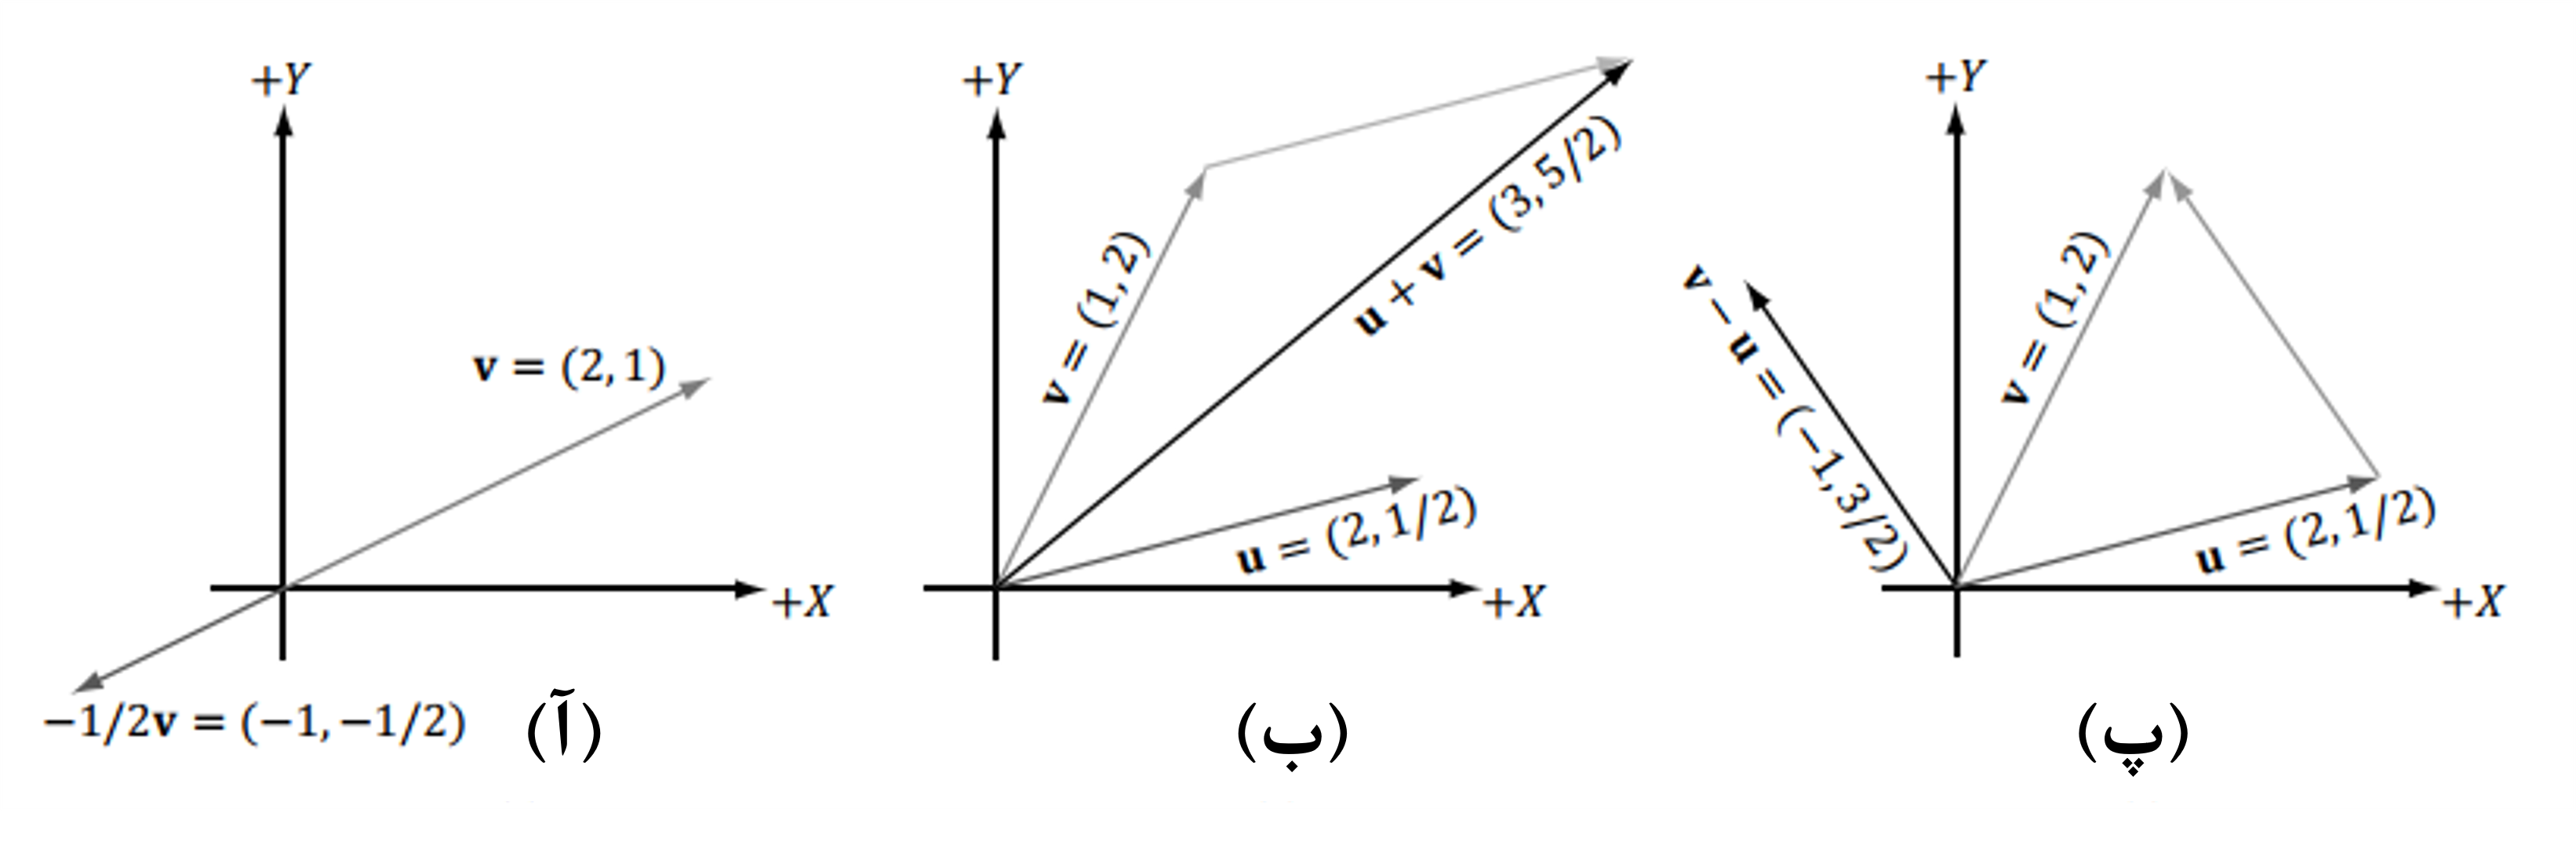
\includegraphics[width=\textwidth]{Images/4/4.Session.1.1.6}
            \caption{(آ) تفسیر هندسی ضرب اسکالر. (ب) تفسیر هندسی جمع بردار. ج) تفسیر هندسی تفریق بردار.}
            \label{fig:4.Session.1.1.6}
        \end{figure}

        \begin{figure}[H]
            \centering
            \setlength{\belowcaptionskip}{-10pt}
            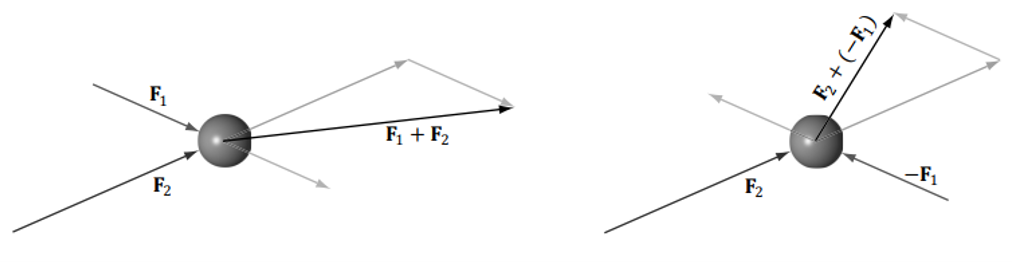
\includegraphics[width=\textwidth]{Images/4/4.Session.1.1.7}
            \caption{نیروهای اعمال شده به یک توپ. نیروها با استفاده از جمع بردار ترکیب می شوند تا نیروی برآیند به دست آید.}
            \label{fig:4.Session.1.1.7}
        \end{figure}
    \end{spacing}
}

%\section{
%    \huge
%
%    \textbf{بردارهای طول و واحد}
%}
%\textbf{\vspace{7pt}}
%{
%    \Large
%    \begin{spacing}{1.5}
%        از نظر هندسی اندازه ی یک بردار، طول پاره خطی جهت دار است.
%        اندازه ی یک بردار را با خط های عمودی دوتایی نشان می دهیم
%        (به عنوان مثال، $\norm{u}$ اندازه ی $\textbf{u}$ را نشان می دهد).
%        حالا با توجه به بردار $\textbf{u}=(x,y,z)$، می‌خواهیم بزرگی آن را به صورت جبری محاسبه کنیم.
%        اندازه ی یک بردار سه بعدی را می توان با دو بار اعمال قضیه فیثاغورث محاسبه کرد.
%        شکل \ref{fig:4.Session.1.1.8} را ببینید. ابتدا، ما به مثلث در صفحه xz با اضلاع x، z و وتر a نگاه می کنیم.
%
%        \begin{figure}[H]
%            \centering
%            \setlength{\belowcaptionskip}{-10pt}
%            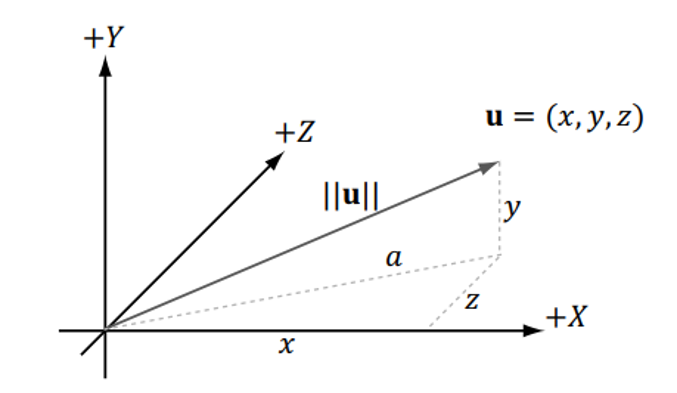
\includegraphics[width=0.5\textwidth]{Images/4/4.Session.1.1.8}
%            \caption{طول سه بعدی یک بردار را می توان با دو بار اعمال قضیه فیثاغورث محاسبه کرد.}
%            \label{fig:4.Session.1.1.8}
%        \end{figure}
%
%        از قضیه فیثاغورث، $a=\sqrt{\displaystyle x^2+z^2}$ داریم.
%        حالا به مثلث با ضلع های \lr{a}، \lr{y} و وتر $\norm{u}$ نگاه کنید از قضیه فیثاغورث دوباره به فرمول اندازه ی زیر می رسیم:
%
%        قضیه*****
%
%        \begin{center}
%            $\norm{\textbf{u}}=\sqrt{\displaystyle y^2+a^2}=\sqrt{\displaystyle y^2+(\sqrt{\displaystyle x^2+z^2})^2}=\sqrt{\displaystyle x^2+y^2+z^2}$
%        \end{center}
%
%        برای برخی از استفاده ها، ما به طول یک بردار اهمیتی نمی دهیم زیرا می خواهیم از بردار برای نمایش یک جهت خالص استفاده کنیم.
%        می خواهیم طول چنین بردارهایی با فقط یک جهت دقیقاً 1 باشد.
%        وقتی طول واحد برداری را می سازیم، می گوییم که بردار را نرمال کرده ایم.
%        می توانیم یک بردار را با تقسیم هر یک از اجزای بر بزرگی آن ، نرمال کنیم:
%
%        قضیه*****
%
%        \begin{center}
%            $\hat{\textbf{u}}=\frac{\displaystyle\textbf{u}}{\displaystyle\norm{\textbf{u}}}=\left(\frac{\displaystyle x}{\displaystyle\norm{\textbf{u}}},
%            \frac{\displaystyle y}{\displaystyle\norm{\textbf{u}}}, \frac{\displaystyle z}{\displaystyle\norm{\textbf{u}}}\right)$
%        \end{center}
%
%        برای تأیید صحت این فرمول، می توانیم طول $\hat{\textbf{u}}$ را محاسبه کنیم
%
%        \begin{center}
%            $\norm{\hat{\textbf{u}}}=\sqrt{\left(\frac{\displaystyle x}{\displaystyle\norm{\textbf{u}}}\right)^2,
%                \left(\frac{\displaystyle y}{\displaystyle\norm{\textbf{u}}}\right)^2,
%                \left(\frac{\displaystyle z}{\displaystyle\norm{\textbf{u}}}\right)^2}=\frac{\displaystyle x^2+y^2+z^2}{\displaystyle\sqrt{\norm{\textbf{u}}^2}}
%            =\frac{\displaystyle\norm{\textbf{u}}}{\displaystyle\norm{\textbf{u}}}=1$
%        \end{center}
%
%
%        پس \hat{\textbf{u}} در واقع یک بردار واحد است.
%
%        مثال***
%
%        بردار $\textbf{v}=(-1,3,4)$ را نرمال کنید. داریم $\norm{\textbf{v}}=\sqrt{\displaystyle (-1)^2+3^2+4^2}=\sqrt{26}$. پس:
%
%        \begin{center}
%            $\hat{\textbf{v}}=\frac{\displaystyle\textbf{v}}{\displaystyle\norm{\textbf{v}}}=\left(-\frac{\displaystyle 1}{\displaystyle\sqrt{26}},
%            \frac{\displaystyle 3}{\displaystyle\sqrt{26}}, \frac{\displaystyle 4}{\displaystyle\sqrt{26}}\right)$
%        \end{center}
%
%        برای تأیید اینکه $\hat{\textbf{v}}$ واقعاً یک بردار واحد است، طول آن را محاسبه می کنیم:
%
%        \begin{center}
%            $\norm{\hat{\textbf{v}}}=\sqrt{\left(-\frac{\displaystyle 1}{\displaystyle\sqrt{26}}\right)^2,
%                \left(\frac{\displaystyle 3}{\displaystyle\sqrt{26}}\right)^2, \left(\frac{\displaystyle 4}{\displaystyle\sqrt{26}}\right)^2}=
%            \sqrt{\displaystyle\frac{\displaystyle 1}{\displaystyle 26}+\frac{\displaystyle 9}{\displaystyle 26}+\frac{\displaystyle 16}{\displaystyle 26}}=\sqrt{\displaystyle 1}=1$
%        \end{center}
%
%    \end{spacing}
%}
%
%\section{
%    \huge
%
%    \textbf{ضرب داخلی}
%}
%\textbf{\vspace{7pt}}
%{
%    \Large
%    \begin{spacing}{1.5}
%        ضرب نقطه ای (داخلی) شکلی از ضرب برداری است که منجر به یک مقدار اسکالر می شود.
%        به همین دلیل، گاهی اوقات از آن به عنوان یک ضرب اسکالر یاد می شود.
%        فرض کنید $\textbf{u}=(u_{x},u_{y},u_{z})$ و  $\textbf{v}=(v_{x},v_{y},v_{z})$،
%        پس حاصل ضرب داخلی به صورت زیر تعریف می‌شود:
%
%        \begin{center}
%            $\textbf{u}\cdot\textbf{v}=u_{x}v_{x}+u_{y}v_{y}+u_{z}v_{z}$
%        \end{center}
%
%        به عبارت دیگر ، ضرب داخلی مجموع ضرب های اجزای مربوطه ست.
%
%        همچنین تعریف ضرب داخلی معنای هندسی آشکاری ارائه نمی دهد.
%        با استفاده از قانون کسینوس (به تمرین ***** مراجعه کنید)، می توانیم رابطه ای را پیدا کنیم که در آن $\theta$ زاویه بین بردارهای $\textbf{u}$ و $\textbf{v}$ است به طوری که $0\leq\theta\leq\pi$؛ شکل ****** را ببینید.
%
%        \begin{center}
%            $\textbf{u}\cdot\textbf{v}=\norm{\textbf{u}}\norm{\textbf{v}}\cos\theta$
%        \end{center}
%
%        بنابراین، معادله ***** می گوید که حاصلضرب نقطه ای بین دو بردار، کسینوس زاویه بین آنها است که با بزرگی بردارها ضرب شده است.
%        به خصوص، اگر هر دو بردار $\textbf{u}$ و $\textbf{v}$ بردار واحد باشند،
%        آنگاه $\textbf{u}\cdot\textbf{v}$ کسینوس زاویه بین آنهاست (یعنی $\textbf{u}\cdot\textbf{v}=\cos\theta$).
%        معادله ***** برخی از ویژگی های هندسی مفید ضرب داخلی را در اختیار ما قرار می دهد:
%
%        \begin{figure}[H]
%            \centering
%            \setlength{\belowcaptionskip}{-10pt}
%            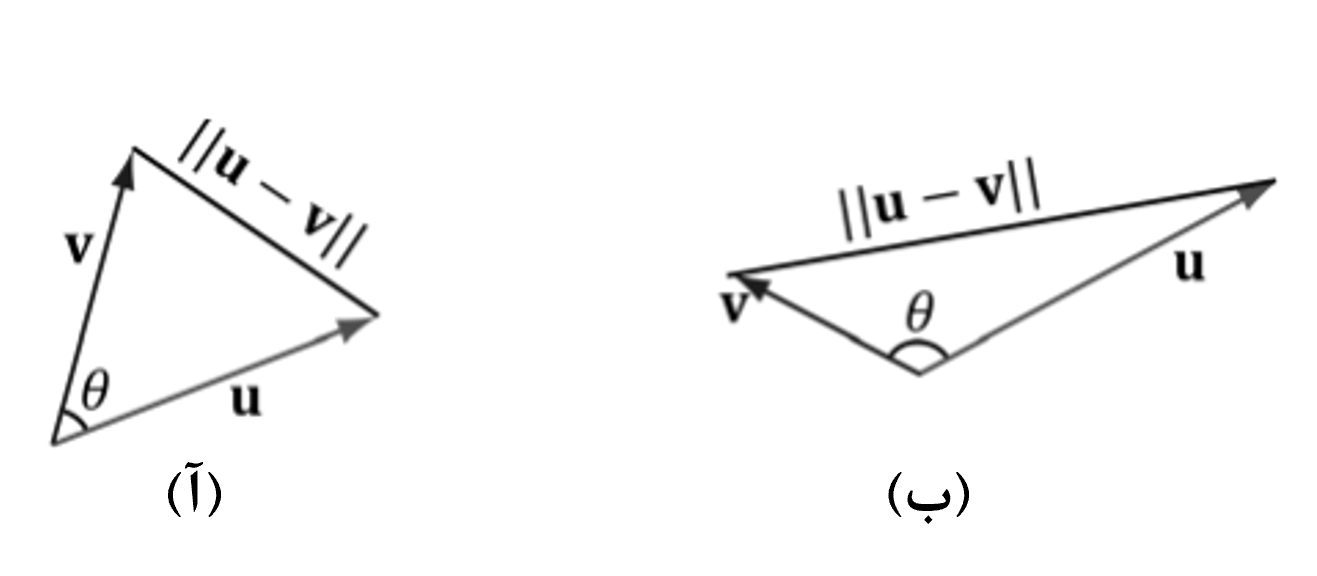
\includegraphics[width=0.5\textwidth]{Images/4/4.Session.1.1.9}
%            \caption{در شکل سمت چپ، زاویه $\theta$ بین $\textbf{u}$ و $\textbf{v}$ یک زاویه تند است.
%            در شکل سمت راست، زاویه $\theta$ بین $\textbf{u}$ و $\textbf{v}$ یک زاویه منفرجه (باز) است.
%            وقتی به زاویه بین دو بردار اشاره می کنیم، همیشه منظورمان کوچکترین زاویه است،
%            یعنی زاویه $\theta$ به طوری که $0\leq\theta\leq\pi$.}
%            \label{fig:4.Session.1.1.9}
%        \end{figure}
%
%        \begin{enumerate}
%            \item {اگر $\textbf{u}\cdot\textbf{v}=0$، در نتیجه $\textbf{u}\perp\textbf{v}$ (یعنی بردار ها بر هم عمودند).}
%            \item {اگر $\textbf{u}\cdot\textbf{v}>0$، در نتیجه زاویه ی بین \theta و دو بردار کمتر از 90 درجه ست (یعنی بردار ها با هم زاویه ی تند میسازند).}
%            \item {اگر $\textbf{u}\cdot\textbf{v}<0$، در نتیجه زاویه ی بین \theta و دو بردار بیشتر از 90 درجه ست (یعنی بردار ها با هم زاویه ی منفرجه میسازند).}
%        \end{enumerate}
%
%        مثال***
%        فرض کنید $\textbf{u}=(1,2,3)$ و $\textbf{v}=(-4,0,-1)$ باشند. زوایه ی بین $\textbf{u}$ و $\textbf{v}$ را پیدا کنید.
%        ابتدا موارد زیر را محاسبه میکنیم:
%
%        \begin{center}
%            $\textbf{u}\cdot\textbf{v}=(1,2,3)\cdot(-4,0,-1)=-4-3=-7$
%
%            $\norm{\textbf{u}}=\sqrt{\displaystyle 1^2+2^2+3^2}=\sqrt{\displaystyle 14}$
%
%            $\norm{\textbf{v}}=\sqrt{\displaystyle (-4)^2+0^2+(-1)^2}=\sqrt{\displaystyle 17}$
%        \end{center}
%
%        حالا ، قضیه ی ***** را برای حل \theta اعمال میکنیم:
%
%        \begin{center}
%            $\cos\theta=\frac{\displaystyle\textbf{u}\cdot\textbf{v}}{\displaystyle\norm{\textbf{v}}\norm{\textbf{u}}}=\frac{\displaystyle -7}{\displaystyle \sqrt{\displaystyle 14}\sqrt{\displaystyle 17}}$
%
%            $\theta=\cos^-1\frac{\displaystyle -7}{\displaystyle \sqrt{\displaystyle 14}\sqrt{\displaystyle 17}}\thickapprox117^\circ$
%        \end{center}
%
%
%        مثال***
%
%        شکل ***** را در نظر بگیرید.
%        با توجه به $\textbf{v}$ و بردار واحد $\textbf{n}$، فرمولی برای $\textbf{p}$ بر حسب $\textbf{v}$ و $\textbf{n}$ با استفاده از ضرب داخلی پیدا کنید.
%        ابتدا، از شکل مشاهده کنید که عدد اسکالر $\textbf{k}$ وجود دارد
%        که $\textbf{p}=k\textbf{n}$؛ علاوه بر این، از آنجایی که ما $\norm{\textbf{u}}=1$ فرض کردیم،
%        داریم $\norm{\textbf{p}}=\norm{k\textbf{n}}=\abs{k}\norm{\textbf{n}}=\abs{k}$.
%        (توجه داشته باشید که $k$ ممکن است منفی باشد اگر و تنها اگر $\textbf{p}$ و $\textbf{n}$ در جهت مخالف قرار گیرند.)
%        با استفاده از مثلثات، داریم که $k=\norm{\textbf{v}}\cos\theta$؛
%        بنابراین، $\textbf{p}=k\textbf{n}=(\norm{\textbf{v}}\cos\theta)\textbf{n}$.
%        با این حال، از آنجایی که \textbf{n} یک بردار واحد است، می توانیم این را به روش دیگری بگوییم:
%
%        \begin{center}
%            $\textbf{p}=(\norm{\textbf{v}}\cos\theta)\textbf{n}=(\norm{\textbf{v}}\cdot 1\cos\theta)\textbf{n}=(\norm{\textbf{v}}\norm{\textbf{n}}\cos\theta)\textbf{n}=(\textbf{v}\cdot\textbf{n})\textbf{n}$
%        \end{center}
%
%        به طور خاص، این $k=\textbf{v}\cdot\textbf{n}$ را نشان می دهد که تفسیر هندسی $\textbf{v}\cdot\textbf{n}$ را هنگامی که $\textbf{n}$ یک بردار واحد است، نشان می دهد. ما $\textbf{p}$ را تصویر متعامد/قائم (\lr{orthogonal projection}) $\textbf{v}$ روی $\textbf{n}$ می نامیم و معمولاً به شکل زیر نشان داده می شود:
%
%        \begin{center}
%            $\textbf{p}=proj_{n}(\textbf{v})$
%        \end{center}
%
%        اگر $\textbf{v}$ را به عنوان نیرو تعبیر کنیم، $\textbf{p}$ را می توان به عنوان بخشی از نیروی $\textbf{v}$ در نظر گرفت که در جهت $\textbf{n}$ عمل می کند.
%        به همین ترتیب، بردار $\textbf{w}=perp_{n}(\textbf{v})=\textbf{v}-\textbf{p}$ بخشی از نیروی $\textbf{v}$ است که در جهت $\textbf{n}$ متعامد عمل می کند
%        (به همین دلیل است که آن را با $perp_{n}(\textbf{v})$ برای عمود نشان می دهیم).
%        مشاهده کنید که $\textbf{v}=\textbf{p}+\textbf{w}=proj_{n}(\textbf{v})+perp_{n}(\textbf{v})$ که می گوییم بردار $\textbf{v}$ را به مجموع دو بردار متعامد $\textbf{p}$ و $\textbf{w}$ تجزیه کرده ایم.
%
%        اگر $\textbf{n}$ طول واحد نباشد، همیشه می‌توانیم ابتدا آن را نرمال کنیم تا طول آن را واحد کنیم.
%        جایگزینی $\textbf{n}$ با بردار واحد $\frac{\displaystyle\textbf{n}}{\norm{\textbf{n}}}$ فرمول تصویر کلی تری را به ما می دهد:
%
%        \begin{center}
%            $\textbf{p}=proj_{n}(\textbf{v})=\left( \textbf{v}\cdot\frac{\displaystyle\textbf{n}}{\norm{\textbf{n}}} \right)\frac{\displaystyle\textbf{n}}{\norm{\textbf{n}}}=\frac{\displaystyle(\textbf{v}\cdot\textbf{n})}{\norm{\textbf{n}}^2}\textbf{n}$
%        \end{center}
%
%        \begin{figure}[H]
%            \centering
%            \setlength{\belowcaptionskip}{-10pt}
%            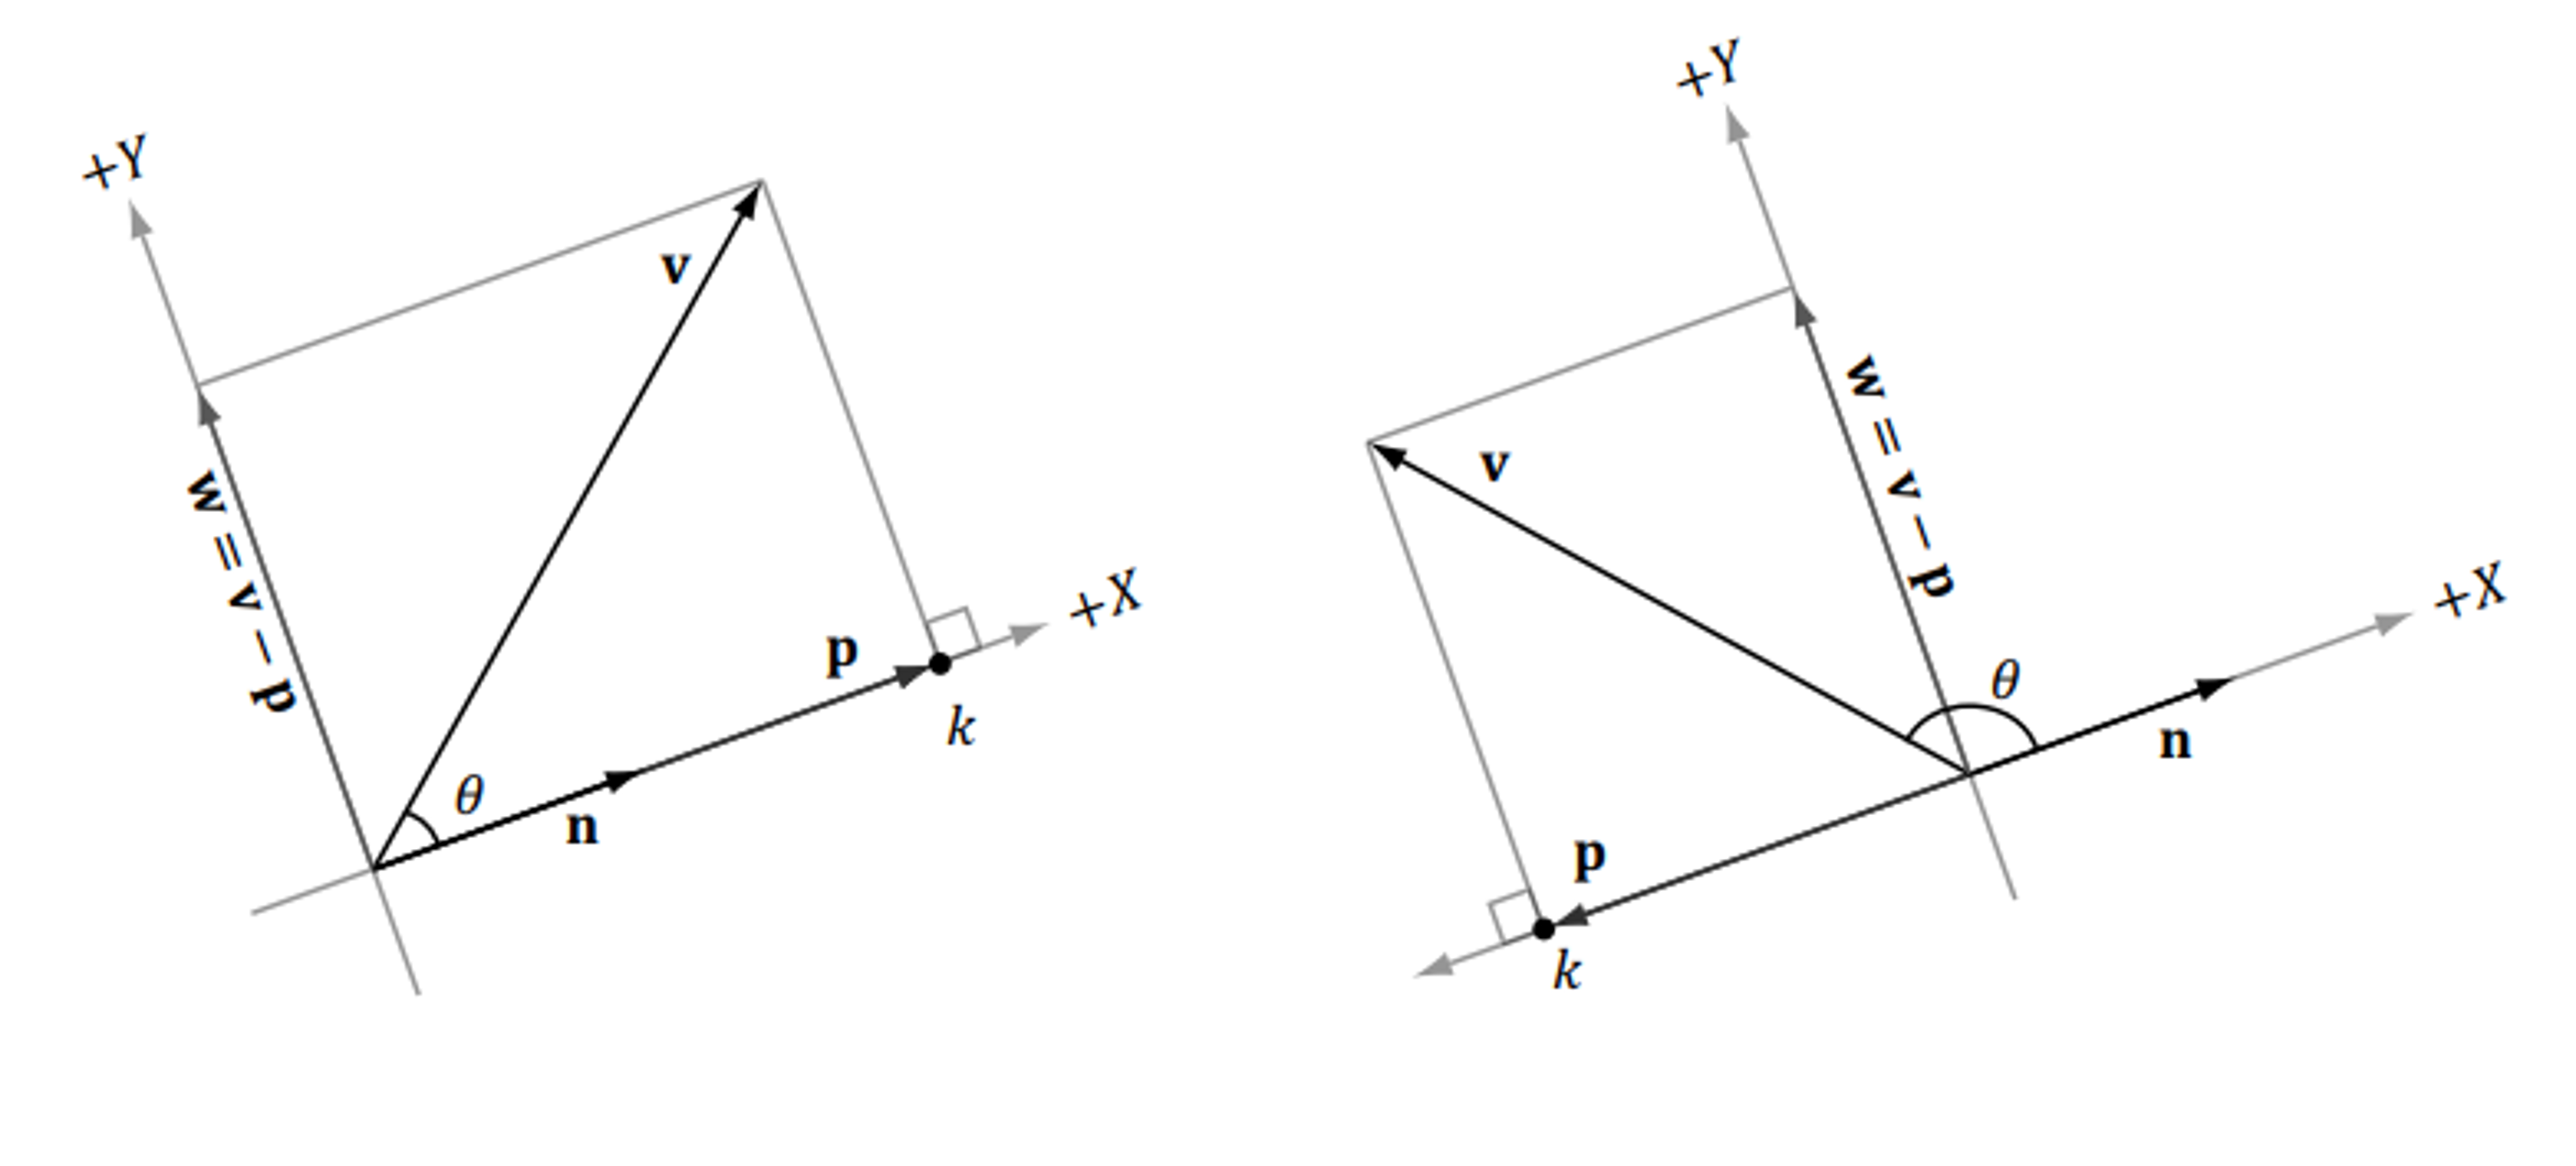
\includegraphics[width=0.5\textwidth]{Images/4/4.Session.1.1.10}
%            \caption{تصویر متعامد/قائم $\textbf{v}$ روی $\textbf{n}$.}
%            \label{fig:4.Session.1.1.10}
%        \end{figure}
%    \end{spacing}
%}
%
%\subsection{\textbf{\LARGE متعامد سازی}}
%{
%    \Large
%    \begin{spacing}{1.5}
%        مجموعه ای از بردارها ${\textbf{v}_{0},...,\textbf{v}_{n-1}}$ متعامد نامیده می شود که بردارها همگی متعامد (هر بردار در مجموعه نسبت به هر بردار دیگری در مجموعه متعامد باشد) و طول واحد باشند.
%        گاهی اوقات ما مجموعه ای از بردارها را داریم که تقریباً متعارف هستند، اما نه کاملاً.
%        یک کار متداول این است که مجموعه را متعامد سازی کنید تا یک مجموعه ی متعامد شود.
%        در گرافیک کامپیوتری سه بعدی ممکن است با یک مجموعه متعارف شروع کنیم، اما به دلیل مسائل مربوط به دقت عددی، مجموعه به تدریج غیرمتعارف شود.
%        ما عمدتاً با موارد دو بعدی و سه بعدی این مشکل (یعنی مجموعه هایی که به ترتیب شامل دو و سه بردار هستند) سروکار داریم.
%
%        ابتدا مورد دو بعدی ساده تر را بررسی می کنیم.
%        فرض کنید مجموعه بردارهای ${\textbf{v}_{0},\textbf{v}_{1}}$ را داریم که می‌خواهیم آن‌ها را به یک مجموعه متعامد ${\textbf{w}_{0},\textbf{w}_{1}}$ تبدیل کنیم،
%        همانطور که در شکل ***** نشان داده شده است.
%        ما با $\textbf{w}_{0}=\textbf{v}_{0}$ شروع کرده و $\textbf{v}_{1}$ را تغییر میدهیم تا آن را به $\textbf{w}_{0}$ متعامد کنیم.
%        این کار با تفریق کردن بخشی از $\textbf{v}_{1}$ که در جهت $\textbf{w}_{0}$  عمل می کند، انجام می شود:
%
%        \begin{center}
%            $\textbf{w}_{1}=\textbf{v}_{1}-proj_{\textbf{w}_{0}}(\textbf{v}_{1})$
%        \end{center}
%
%        \begin{figure}[H]
%            \centering
%            \setlength{\belowcaptionskip}{-10pt}
%            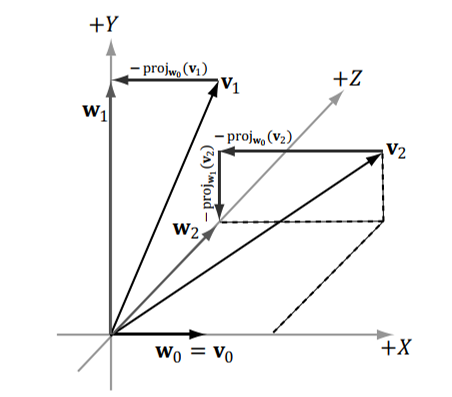
\includegraphics[width=0.5\textwidth]{Images/4/4.Session.1.1.11}
%            \caption{متعامد سازی دو بعدی}
%            \label{fig:4.Session.1.1.11}
%        \end{figure}
%
%        اکنون مجموعه ای متعامد از بردارها داریم ${\textbf{w}_{0},\textbf{w}_{1}}$.
%        آخرین مرحله برای ساخت مجموعه متعارف نرمال کردن $\textbf{w}_{0}$ و $\textbf{w}_{1}$ برای ایجاد طول واحد است.
%
%        حالت سه بعدی به همان شکل مورد دو بعدی اما با مراحل بیشتر است.
%        فرض کنید مجموعه بردارهای ${\textbf{v}_{0},\textbf{v}_{1},\textbf{v}_{2}}$ را داریم که می‌خواهیم آنها را یک مجموعه متعامد ${\textbf{w}_{0},\textbf{w}_{1},\textbf{w}_{2}}$ کنیم، مطابق شکل *****.
%        ما با $\textbf{w}_{0}=\textbf{v}_{0}$ شروع می کنیم و $\textbf{v}_{1}$ را تغییر می دهیم تا به $\textbf{w}_{0}$ متعامد شود.
%        این کار با کم کردن بخشی از $\textbf{v}_{1}$ که در جهت $\textbf{w}_{0}$ عمل می کند انجام می شود:
%
%        \begin{center}
%            $\textbf{w}_{1}=\textbf{v}_{1}-proj_{\textbf{w}_{0}}(\textbf{v}_{1})$
%        \end{center}
%
%        \begin{figure}[H]
%            \centering
%            \setlength{\belowcaptionskip}{-10pt}
%            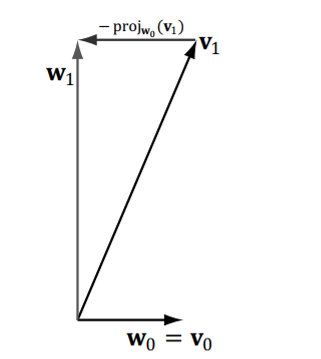
\includegraphics[width=0.5\textwidth]{Images/4/4.Session.1.1.12}
%            \caption{متعامد سازی سه بعدی}
%            \label{fig:4.Session.1.1.12}
%        \end{figure}
%
%        در مرحله بعد، $\textbf{v}_{2}$ را تغییر می دهیم تا آن را متعامد به $\textbf{w}_{0}$ و $\textbf{w}_{1}$ کنیم.
%        این کار با تفریق کردن بخشی از $\textbf{v}_{2}$ که در جهت $\textbf{w}_{0}$ عمل می کند و بخشی از $\textbf{v}_{2}$ که در جهت $\textbf{w}_{1}$ عمل می کند، انجام می شود:
%
%        \begin{center}
%            $\textbf{w}_{2}=\textbf{v}_{2}-proj_{\textbf{w}_{0}}(\textbf{v}_{2})-proj_{\textbf{w}_{1}}(\textbf{v}_{2})$
%        \end{center}
%
%        اکنون یک مجموعه متعامد از بردارها داریم ${\textbf{w}_{0},\textbf{w}_{1},\textbf{w}_{2}}$.
%        آخرین مرحله برای ساخت مجموعه متعامد نرمال کردن $\textbf{w}_{0}$، $\textbf{w}_{1}$ و $\textbf{w}_{2}$ است تا طول آنها را واحد کنیم.
%
%        برای حالت کلی $\textbf{n}$ بردار ${\textbf{v}_{0},...,\textbf{v}_{n-1}}$ که می‌خواهیم آنها را به یک مجموعه متعامد تبدیل کنیم { w0، ...، wn1}، ما روال زیر را داریم که معمولاً فرآیند متعامدسازی گرام اشمیت (\lr{Gram-Schmidt}) نامیده می شود:
%
%        \begin{center}
%            گام پایه: $\textbf{w}_{0}=\textbf{v}_{0}$ قرار میدهیم
%
%            به ازای $1\leq i\leq n-1$ ، $\textbf{w}_{i}=\textbf{v}_{i}-\sum_{j=1}^{i-1}proj_{\textbf{w}_{j}}(\textbf{v}_{i})$ قرار میدهیم
%
%            گام نرمال سازی: $\textbf{w}_{i}=\frac{\displaystyle\textbf{w}_{i}}{\displaystyle\norm{\textbf{w}_{i}}}$ قرار میدهیم
%        \end{center}
%
%        دوباره، ایده شهودی این است که وقتی یک بردار $\textbf{v}_{i}$ را از مجموعه ورودی انتخاب می کنیم تا به مجموعه متعارف اضافه کنیم،
%        باید اجزای $\textbf{v}_{i}$ را که در جهت بردارهای دیگر عمل کرده و از قبل در مجموعه متعامد قرار دارند ($\textbf{w}_{0},\textbf{w}_{1},...,\textbf{w}_{i-1}$) را کم کنیم.
%        این کار باعث اطمینان حاصل از این که بردار جدید اضافه شده با سایر بردارهای موجود در مجموعه متعامد، متعامد باشد، میشود.
%    \end{spacing}
%}
%
%\section{
%    \huge
%
%    \textbf{ضرب خارجی}
%}
%\textbf{\vspace{7pt}}
%{
%    \Large
%    \begin{spacing}{1.5}
%        شکل دوم بردار ضرب ریاضی، ضرب خارجی است.
%        بر خلاف ضرب داخلی که به یک اسکالر ختم می‌شود، ضرب خارجی به یک بردار دیگر ختم می‌شود.
%        علاوه بر این، ضرب خارجی فقط برای بردارهای سه بعدی تعریف شده است (در واقع ضرب خارجی دو بعدی وجود ندارد).
%        با ضرب خارجی دو بردار سه بعدی u و v، بردار دیگری به دست می‌آید،که w متعامد به u و v است.
%        شکل ***** را ببینید.
%        اگر $\textbf{u}=(u_{x},u_{y},u_{z})$ و  $\textbf{v}=(v_{x},v_{y},v_{z})$ باشد، آنگاه ضرب خارجی به این صورت محاسبه می‌شود:
%
%        \begin{center}
%            $\textbf{w}=\textbf{u}\times\textbf{v}=(u_{y}v_{z}-u_{z}v_{y}, u_{z}v_{x}-u_{x}v_{z}, u_{x}v_{y}-u_{y}v_{z})$
%        \end{center}
%
%        \begin{theo}{thm:pythagoras}
%            \Large
%            اگر در سیستم مختصات راستگرد کار می کنید، پس از قانون شست دست راست استفاده می کنید:
%            اگر دست راست خود را طوری بگیرید که انگشتان در جهت بردار اول u باشد و سپس انگشتان خود را به سمت v با زاویه ی $0\leq\theata\leq \pi$ خم کنید، انگشت شست شما در جهت $\textbf{w}=\textbf{u}\times\textbf{v}$ قرار می گیرد.
%        \end{theo}
%
%        \begin{figure}[H]
%            \centering
%            \setlength{\belowcaptionskip}{-10pt}
%            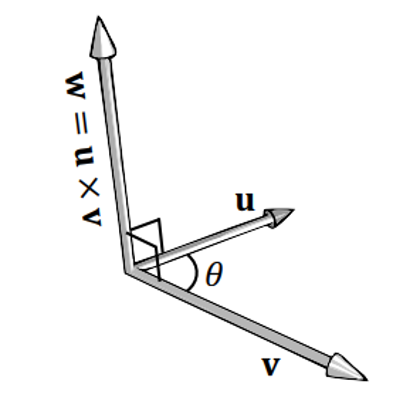
\includegraphics[width=0.5\textwidth]{Images/4/4.Session.1.1.13}
%            \caption{ضرب خارجی دو بردار سه بعدی $\textbf{u}$ و $\textbf{v}$ بردار دیگر $\textbf{w}$ را به دست می آورد که متعامد با $\textbf{u}$ و $\textbf{v}$ است.
%            اگر دست چپ خود را طوری بگیرید که انگشتان در جهت بردار اول u باشد و سپس انگشتان خود را به سمت v با زاویه ی $0\leq\theata\leq \pi$ خم کنید، انگشت شست شما در جهت $\textbf{w}=\textbf{u}\times\textbf{v}$ قرار می گیرد. به این قانون شست چپ می گویند.}
%            {متعامد سازی سه بعدی}
%            \label{Images/4/4.Session.1.1.13}
%        \end{figure}
%
%        مثال***
%
%        فرض کنید $\textbf{u}=(1,2,3)$ و $\textbf{v}=(1,2,3)$ باشد. سپس $\textbf{w}=\textbf{u}\times\textbf{v}$ و $\textbf{z}=\textbf{v}\times\textbf{z}$ را محاسبه کنید. قضیه ی ***** را اعمال میکنیم:
%
%        \begin{center}
%            \begin{split}
%                $\textbf{w}&=\textbf{u}\times\textbf{v}\\
%                &=(2,1,3)\times(2,0,0)\\
%                &=(1\cdot 0-3\cdot 0, 3\cdot 2-2\cdot 0, 2\cdot 0-1\cdot 2)\\
%                &=(0,6,-2)$
%            \end{split}
%        \end{center}
%
%        و
%
%        \begin{center}
%            \begin{split}
%                $\textbf{z}&=\textbf{v}\times\textbf{u}\\
%                &=(2,0,0)\times(2,1,3)\\
%                &=(0\cdot 3-0\cdot 1, 0\cdot 2-2\cdot 3, 2\cdot 1-0\cdot 2)\\
%                &=(0,6,-2)$
%            \end{split}
%        \end{center}
%
%        این نتیجه یک چیز را روشن می کند، به طور کلی $\textbf{u}\times\textbf{v}\neq\textbf{v}\times\textbf{u}$. بنابراین، می گوییم که ضرب خارجی خاصیت جابجایی ندارد.
%        در واقع می توان نشان داد که $\textbf{u}\times\textbf{v}=-\textbf{v}\times\textbf{u}$. شما می توانید بردار به دست آمده از ضرب خارجی را با قانون انگشت شست چپ تعیین کنید.
%        اگر ابتدا انگشتان خود را در جهت بردار اول نشانه بگیرید و سپس انگشتان خود را به سمت بردار دوم خم کنید (همیشه مسیر را با کوچکترین زاویه انتخاب کنید)، همانطور که در شکل ***** نشان داده شده است، انگشت شست شما در جهت بردار حاصل قرار می گیرد.
%
%        برای نشان دادن اینکه $\textbf{w}$ متعامد به $\textbf{u}$ و $\textbf{w}$ متعامد بر $\textbf{v}$ است،
%        از ***** یادآوری می کنیم که اگر$\textbf{u}\times\textbf{v}=0$ باشد،
%        آنگاه $\textbf{u}\perp\textbf{v}$ است (یعنی بردارها متعامد هستند). زیرا
%
%        \begin{center}
%            $\textbf{w}\times\textbf{u}=(0,6,-2)\cdot(2,1,3)=0\cdot 2+6\cdot 1+(-2)\cdot 3=0$
%
%            و
%
%            $\textbf{w}\times\textbf{v}=(0,6,-2)\cdot(2,0,0)=0\cdot 2+6\cdot 0+(-2)\cdot 0=0$
%        \end{center}
%
%        نتیجه می گیریم که $\textbf{w}$ متعامد به $\textbf{u}$ و $\textbf{w}$ متعامد بر $\textbf{v}$ است.
%    \end{spacing}
%}
%
%\subsection{\textbf{\LARGE ضرب خارجی شبه دو بعدی}}
%{
%    \Large
%    \begin{spacing}{1.5}
%        ضرب خارجی به ما امکان می دهد یک بردار متعامد به دو بردار سه بعدی داده شده را پیدا کنیم.
%        در دوبعدی وضعیت مشابهی نداریم،
%        اما با توجه به بردار دوبعدی $\textbf{u}=u_{x},u_{y}$ پیدا کردن بردار $\textbf{v}$ متعامد به $\textbf{u}$ می‌تواند مفید باشد.
%        شکل ****** شکل هندسی ای را نشان می دهد که از آن $\textbf{v}=-u_{y},u_{x}$ پیدا میشود.
%        اثبات آن ساده است:
%
%        \begin{center}
%            $\textbf{u}\cdot\textbf{v}=(u_{x},u_{y})\cdot(-u_{y},u_{x})=-u_{x}u_{y}+u_{y}u_{x}=0$
%        \end{center}
%
%        بنابراین $\textbf{u}\perp\textbf{v}$.
%        مشاهده کنید که $\textbf{u}\cdot-\textbf{v}=u_{x}u_{y}+u_{y}(-u_{x})=0$، بنابراین $\textbf{u}\perp-\textbf{v}$ را نیز داریم.
%
%        \begin{figure}[H]
%            \centering
%            \setlength{\belowcaptionskip}{-10pt}
%            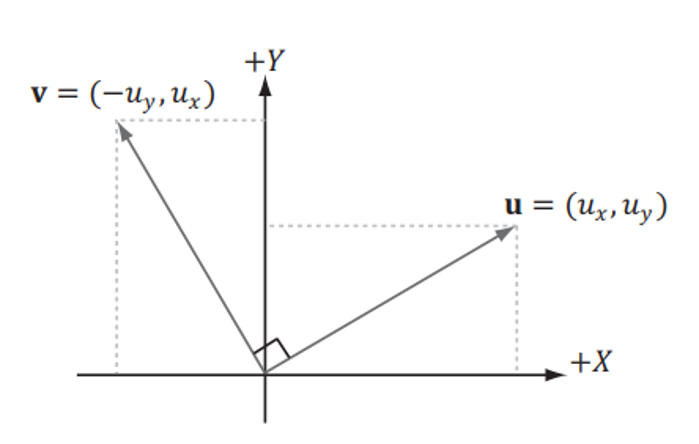
\includegraphics[width=0.5\textwidth]{Images/4/4.Session.1.1.14}
%            \caption{ضرب خارجی شبه دوبعدی یک بردار $\textbf{u}$ به بردار متعامد $\textbf{v}$ ختم می شود.}
%            \label{Images/4/4.Session.1.1.14}
%        \end{figure}
%    \end{spacing}
%}
%
%\subsection{\textbf{\LARGE متعامد سازی با ضرب خارجی}}
%{
%    \Large
%    \begin{spacing}{1.5}
%        در ******، ما روشی برای متعامد کردن مجموعه ای از بردارها با استفاده از فرآیند گرام اشمیت را مشاهده کردیم.
%        برای سه بعدی، استراتژی دیگری برای متعامد کردن مجموعه ای از بردارها $\textbf{v}_{0},\textbf{v}_{1},\textbf{v}_{2}$ وجود دارد که متعارف هستند،
%        اما ممکن است به دلیل خطاهای انباشته شده در دقت عددی با استفاده از ضرب خارجی، غیرمتعارف شوند.
%        برای شکل هندسی این فرآیند به شکل ****** مراجعه کنید:
%
%        \begin{enumerate}
%            \item {$\textbf{w}_{0}=\frac{\displaystyle\textbf{v}_{0}}{\displaystyle\norm{\textbf{v}_{0}}}$ قرار میدهیم}
%            \item {$\textbf{w}_{2}=\frac{\displaystyle\textbf{w}_{0}\times\textbf{v}_{1}}{\displaystyle\norm{\textbf{w}_{0}\times\textbf{v}_{1}}}$ قرار میدهیم}
%            \item {با قرار دادن $\textbf{w}_{1}=\textbf{w}_{2}\times\textbf{w}_{0}$ توسط تمرین ******، $\norm{\textbf{w}_{2}\times\textbf{w}_{0}}=1$ زیرا $\textbf{w}_{2}\perp\textbf{w}_{0}$ و $\norm{\textbf{w}_{2}}=\norm{\textbf{w}_{0}}=1$،
%            بنابراین در این مرحله آخر نیازی به نرمال سازی نداریم.}
%        \end{enumerate}
%
%        در این مرحله، مجموعه بردارهای ${\textbf{w}_{0},\textbf{w}_{1},\textbf{w}_{2}}$ متعامد است.
%
%        \begin{figure}[H]
%            \centering
%            \setlength{\belowcaptionskip}{-10pt}
%            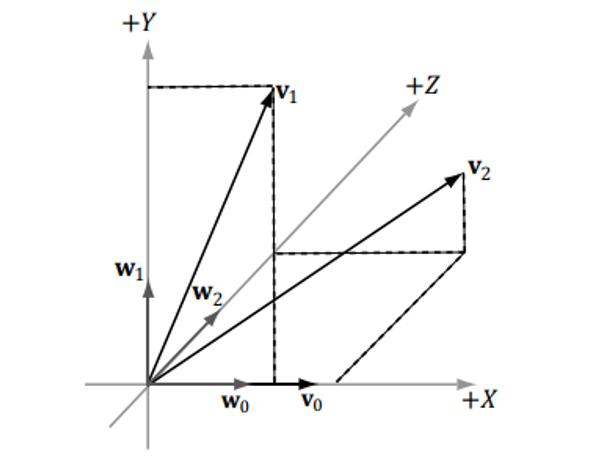
\includegraphics[width=0.5\textwidth]{Images/4/4.Session.1.1.15}
%            \caption {متعامد سازی سه بعدی با ضرب خارجی}
%            \label{Images/4/4.Session.1.1.15}
%        \end{figure}
%
%        \begin{theo}{thm:pythagoras}
%            \Large
%            در مثال بالا، ما با 00$\textbf{w}_{0}=\frac{\displaystyle\textbf{v}_{0}}{\displaystyle\norm{\textbf{v}_{0}}}$ شروع کردیم، به این معنی که هنگام رفتن از $\textbf{v}_{0}$ به $\textbf{w}_{0}$ جهت را تغییر ندادیم،
%            ما فقط طول را تغییر دادیم.
%            با این حال، جهت های $\textbf{w}_{1}$ و $\textbf{w}_{2}$ می تواند به ترتیب با $\textbf{v}_{1}$ و $\textbf{v}_{2}$ متفاوت باشد.
%            بسته به کاربرد خاص، برداری که شما انتخاب میکنید تغییر جهت ندهد ممکن است مهم باشد.
%            به عنوان مثال، در ادامه این کتاب، جهت دوربین را با سه بردار متعامد ${\textbf{v}_{0},\textbf{v}_{1},\textbf{v}_{2}}$ نشان می‌دهیم که بردار سوم $\textbf{v}_{2}$ جهتی را که دوربین به آن نگاه می‌کند، تعریف میکند.
%            هنگامی که این بردارها را متعامد می کنیم، اغلب نمی خواهیم جهت مورد نظر خود را تغییر دهیم،
%            بنابراین الگوریتم فوق را با $\textbf{v}_{2}$ شروع می کنیم و $\textbf{v}_{0}$ و $\textbf{v}_{1}$ را تغییر می دهیم تا بردارها متعامد شوند.
%        \end{theo}
%    \end{spacing}
%}
%
%\section{
%    \huge
%
%    \textbf{نقاط}
%}
%\textbf{\vspace{7pt}}
%{
%    \Large
%    \begin{spacing}{1.5}
%        تاکنون در مورد بردارها بحث کرده ایم که موقعیت ها را توصیف نمی کنند.
%        با این حال، ما همچنین باید موقعیت هایی را در برنامه های سه بعدی خود مشخص کنیم،
%        به عنوان مثال، موقعیت هندسی سه بعدی و موقعیت دوربین مجازی سه بعدی.
%        نسبت به یک سیستم مختصات، می‌توانیم از یک بردار در موقعیت استاندارد (شکل *****) برای نمایش یک موقعیت سه بعدی در فضا استفاده کنیم.
%        ما این بردار را بردار موقعیت می نامیم.
%        در این حالت، محل نوک بردار مشخصه مورد نظر است، نه جهت یا بزرگی.
%        ما از عبارات "بردار موقعیت" و "نقطه" به جای یکدیگر استفاده خواهیم کرد زیرا بردار موقعیت برای شناسایی یک نقطه کافی است.
%
%        \begin{figure}[H]
%            \centering
%            \setlength{\belowcaptionskip}{-10pt}
%            \includegraphics[width=0.5\textwidth]{Images/4/4.Session.1.1.16}
%            \caption {بردار موقعیت، که از مبدا تا نقطه کشیده میشود، به طور کامل محل قرارگیری نقطه را نسبت به سیستم مختصات توصیف می کند.}
%            \label{Images/4/4.Session.1.1.16}
%        \end{figure}
%
%        یکی از مزایای استفاده از بردارها برای نشان دادن نقاط، به ویژه در کد، این است که می‌توانیم عملیات های بردار را انجام دهیم که برای نقاط معنی ندارد.
%        به عنوان مثال، از نظر هندسی، مجموع دو نقطه باید به چه معنا باشد؟
%        از سوی دیگر، برخی از عملیات را می توان به نقاط گسترش داد.
%        به عنوان مثال، ما فاصله ی دو نقطه $\textbf{q}-\textbf{p}$ را برداری از $\textbf{p}$ به $\textbf{q}$ تعریف می کنیم. همچنین، ما یک نقطه $\textbf{p}$ به اضافه بردار $\textbf{v}$ را نقطه ی $\textbf{q}$ تعریف میکنیم که با جابجایی p با بردار v به دست می آید.
%        به راحتی، از آنجایی که ما از بردارها برای نشان دادن نقاط نسبت به یک سیستم مختصات استفاده می‌کنیم، نیازی به کار اضافی برای عملیات نقطه‌ای که قبلاً در مورد آن بحث شد، نیست، زیرا چارچوب جبر برداری از قبل آنها را آماده می‌کند. شکل ***** را ببینید.
%
%        \begin{figure}[H]
%            \centering
%            \setlength{\belowcaptionskip}{-10pt}
%            \includegraphics[width=0.5\textwidth]{Images/4/4.Session.1.1.17}
%            \caption {(آ) فاصله ی دو نقطه $\textbf{q}-\textbf{p}$ برداری از $\textbf{p}$ به $\textbf{q}$ تعریف میشود. (ب) یک نقطه $\textbf{p}$ به اضافه بردار $\textbf{v}$ را نقطه ی $\textbf{q}$ تعریف میکنیم که با جابجایی p با بردار v به دست می آید.}
%            \label{Images/4/4.Session.1.1.17}
%        \end{figure}
%
%        \begin{theo}{thm:pythagoras}
%            \Large
%            در واقع یک روش هندسی معنادار برای تعریف یک مجموع ویژه از نقاط وجود دارد که به آن ترکیب وابسته می گویند، که مانند میانگین وزنی نقاط است.
%        \end{theo}
%    \end{spacing}
%}
%
%\section{
%    \huge
%
%    \textbf{بردار های ریاضی \lr{DirectX}}
%}
%{
%    \Large
%    \begin{spacing}{1.5}
%        در ویندوز 8 و بالاتر، \lr{DirectX Math} یک کتابخانه ریاضی سه بعدی برای برنامه \lr{Direct3D} است که بخشی از \lr{Windows SDK} است.
%        این کتابخانه از مجموعه دستورالعمل \lr{SSE2} (\lr{Streaming SIMD Extensions 2}) استفاده می کند.
%        با رجیسترهای \lr{SIMD} گسترده \lr{128} بیتی (داده‌های چندگانه تک دستورالعمل)، دستورالعمل‌های \lr{SIMD} می‌توانند روی چهار عدد \lr{int} یا عدد \lr{float} \lr{32} بیتی با یک دستورالعمل کار کنند.
%        این برای محاسبات برداری بسیار مفید است. برای مثال، اگر به جمع برداری نگاه کنید:
%
%        \begin{center}
%            $\textbf{u}+\textbf{v}=(u_{x}+v_{x},u_{y}+v_{y},u_{z}+v_{z})$
%        \end{center}
%
%        می بینیم که ما فقط اجزای مربوطه را اضافه می کنیم.
%        با استفاده از \lr{SIMD} می‌توانیم به جای چهار دستور اسکالر، جمع بردار چهار بعدی را با یک دستور \lr{SIMD} انجام دهیم.
%        اگر ما فقط به سه مختصات برای کار سه بعدی نیاز داشته باشیم، همچنان می توانیم از \lr{SIMD} استفاده کنیم، اما مختصات چهارم را نادیده می گیریم.
%        به همین ترتیب، برای دو بعدی، مختصات سوم و چهارم را نادیده می گیریم.
%
%        پوشش ما از کتابخانه ریاضی \lr{DirectX} جامع نیست و ما فقط بخش های کلیدی مورد نیاز برای این کتاب را پوشش می دهیم.
%        برای تمام جزئیات، ما مستندات آنلاین [\lr{DirectXMath}] را توصیه می کنیم.
%        برای خوانندگانی که مایلند بدانند چگونه یک کتابخانه برداری \lr{SIMD} ممکن است به طور بهینه توسعه یابد، و شاید درک کنند که چرا کتابخانه ریاضی \lr{DirectX} برخی از تصمیمات طراحی را اتخاذ کرده است،
%        مقاله \lr{Designing Fast Cross-Platform SIMD Vector Libraries [by Oliveira2010]} را توصیه می کنیم.
%
%        برای استفاده از کتابخانه ریاضی \lr{DirectX}، باید \texttt{#include <DirectXMath.h>} و برای برخی از انواع داده های اضافی \texttt{#include <DirectXPackedVector.h>} را وارد کنید.
%        هیچ فایل کتابخانه ای اضافی وجود ندارد، زیرا تمام کدها به صورت درون خطی در فایل هدر پیاده سازی می شوند.
%        کد \lr{DirectXMath.h} در فضای نام \texttt{DirectX} و کد \lr{DirectXPackedVector.h} در فضای نام \texttt{DirectX::PackedVector} وجود دارد.
%        علاوه بر این، برای پلتفرم \lr{x86} باید \lr{SSE2} را فعال کنید:
%
%        (\textbf{Project Properties > Configuration Properties > C/C++ > Code Generation > Enable Enhanced Instruction Set})
%
%        و برای همه پلتفرم‌ها باید مدل ممیز شناور سریع \lr{/fp:fast} را فعال کنید:
%
%        (\textbf{Project Properties > Configuration Properties > C/C++ > Code Generation > Floating Point Model})
%
%        شما نیازی به فعال کردن \lr{SSE2} برای پلتفرم \lr{x64} ندارید زیرا تمام پردازنده‌های \lr{x64} از \lr{SSE2} (\url{http://en.wikipedia.org/wiki/SSE2}) پشتیبانی می‌کنند.
%    \end{spacing}
%}
%
%\subsection{\textbf{\LARGE انواع بردارها}}
%{
%    \Large
%    \begin{spacing}{1.5}
%        در \lr{DirectX Math}، نوع بردار هسته \texttt{XMVECTOR} است که به رجیسترهای سخت افزاری \lr{SIMD} نگاشت می شود.
%        این یک نوع \lr{128} بیتی است که می تواند چهار \lr{float} \lr{32} بیتی را با یک دستورالعمل \lr{SIMD} پردازش کند.
%        وقتی \lr{SSE2} در دسترس باشد، برای پلتفرم‌های \lr{x86} و \lr{x64} به این صورت تعریف می‌شود که \lr{__m128} یک نوع \lr{SIMD} خاص است.:
%
%        \texttt{typedef __m128 XMVECTOR;}
%
%        هنگام انجام محاسبات، بردارها باید از این نوع باشند تا از \lr{SIMD} استفاده کنند.
%        همانطور که قبلا ذکر شد، ما همچنان از این نوع برای بردارهای دو بعدی و سه بعدی استفاده می کنیم تا از مزایای \lr{SIMD} استفاده کنیم،
%        اما فقط اجزای استفاده نشده را صفر کرده و آنها را نادیده می گیریم.
%
%        \texttt{XMVECTOR} باید \lr{16} بایت تراز شود و این به طور خودکار برای متغیرهای محلی و سراسری انجام می شود.
%        برای اعضای داده کلاس، توصیه می شود به جای آن از \texttt{XMFLOAT2} (\lr{2D})، \texttt{XMFLOAT3} (\lr{3D}) و \texttt{XMFLOAT4} (\lr{4D}) استفاده کنید. این ساختارها در زیر تعریف می شوند:
%
%        \texttt
%        {
%            struct XMFLOAT2
%                {
%                float x;
%                float y;
%                XMFLOAT2() {}
%                XMFLOAT2(float _x, float _y) : x(_x), y(_y) {}
%                explicit XMFLOAT2(_In_reads_(2) const float *pArray) :
%                x(pArray[0]), y(pArray[1]) {}
%                XMFLOAT2& operator= (const XMFLOAT2& Float2)
%                    { x = Float2.x; y = Float2.y; return *this; }
%            };
%        struct XMFLOAT3
%                {
%                float x;
%                float y;
%                float z;
%                XMFLOAT3() {}
%                XMFLOAT3(float _x, float _y, float _z) : x(_x), y(_y), z(_z) {}
%                explicit XMFLOAT3(_In_reads_(3) const float *pArray) :
%                x(pArray[0]), y(pArray[1]), z(pArray[2]) {}
%                XMFLOAT3& operator= (const XMFLOAT3& Float3)
%                    { x = Float3.x; y = Float3.y; z = Float3.z; return *this; }
%            };
%        struct XMFLOAT4
%                {
%                float x;
%                float y;
%                float z;
%                float w;
%                XMFLOAT4() {}
%                XMFLOAT4(float _x, float _y, float _z, float _w) :
%                x(_x), y(_y), z(_z), w(_w) {}
%                explicit XMFLOAT4(_In_reads_(4) const float *pArray) :
%                x(pArray[0]), y(pArray[1]), z(pArray[2]), w(pArray[3]) {}
%                XMFLOAT4& operator= (const XMFLOAT4& Float4)
%                    { x = Float4.x; y = Float4.y; z = Float4.z; w = Float4.w; return
%                *this; }
%            };
%        }
%
%        اما اگر مستقیماً از این انواع برای محاسبات استفاده کنیم، از \lr{SIMD} استفاده نخواهیم کرد.
%        برای استفاده از \lr{SIMD} باید نمونه هایی از این نوع را به نوع \texttt{XMVECTOR} تبدیل کنیم.
%        این کار با توابع بارگیری ریاضی \lr{DirectX} انجام می شود.
%        برعکس، \lr{DirectX} توابع ذخیره سازی را فراهم می کند که برای تبدیل داده ها از \texttt{XMVECTOR} به انواع \texttt{XMFLOATn} در بالا استفاده می شود.
%
%        به طور خلاصه،
%
%        \begin{enumerate}
%            \item {از \texttt{XMVECTOR} برای متغیرهای محلی یا سراسری استفاده کنید.}
%            \item {از \texttt{XMFLOAT2}، \texttt{XMFLOAT3} و \texttt{XMFLOAT4} برای اعضای داده کلاس استفاده کنید.}
%            \item {قبل از انجام محاسبات از توابع بارگذاری برای تبدیل از \texttt{XMFLOATn} به \texttt{XMVECTOR} استفاده کنید.}
%            \item {محاسبات را با نمونه های \texttt{XMVECTOR} انجام دهید.}
%            \item {از توابع ذخیره سازی برای تبدیل از \texttt{XMVECTOR} به \texttt{XMFLOATn} استفاده کنید.}
%        \end{enumerate}
%
%    \end{spacing}
%}
%
%\subsection{\textbf{\LARGE روش های بارگیری و ذخیره سازی}}
%{
%    \Large
%    \begin{spacing}{1.5}
%        ما از روش های زیر برای بارگذاری داده ها از \texttt{XMFLOATn} در \texttt{XMVECTOR} استفاده می کنیم:
%
%        \texttt
%        {
%            // Loads XMFLOAT2 into XMVECTOR
%            XMVECTOR XM_CALLCONV XMLoadFloat2(const XMFLOAT2 *pSource);
%
%        // Loads XMFLOAT3 into XMVECTOR
%        XMVECTOR XM_CALLCONV XMLoadFloat3(const XMFLOAT3 *pSource);
%
%        // Loads XMFLOAT4 into XMVECTOR
%        XMVECTOR XM_CALLCONV XMLoadFloat4(const XMFLOAT4 *pSource);
%        }
%
%        ما از روش های زیر برای ذخیره داده ها از \texttt{XMVECTOR} در \texttt{XMFLOATn} استفاده می کنیم:
%
%        \texttt
%        {
%            // Loads XMVECTOR into XMFLOAT2
%            void XM_CALLCONV XMStoreFloat2(XMFLOAT2 *pDestination, FXMVECTOR V);
%
%        // Loads XMVECTOR into XMFLOAT3
%        void XM_CALLCONV XMStoreFloat3(XMFLOAT3 *pDestination, FXMVECTOR V);
%
%        // Loads XMVECTOR into XMFLOAT4
%        void XM_CALLCONV XMStoreFloat4(XMFLOAT4 *pDestination, FXMVECTOR V);
%        }
%
%        گاهی اوقات ما فقط می خواهیم یک جزء \texttt{XMVECTOR} را دریافت یا تنظیم کنیم. توابع \lr{getter} و \lr{setter} زیر این امر را تسهیل می کنند:
%
%        \texttt
%        {
%            float XM_CALLCONV XMVectorGetX(FXMVECTOR V);
%        float XM_CALLCONV XMVectorGetY(FXMVECTOR V);
%        float XM_CALLCONV XMVectorGetZ(FXMVECTOR V);
%        float XM_CALLCONV XMVectorGetW(FXMVECTOR V);
%        XMVECTOR XM_CALLCONV XMVectorSetX(FXMVECTOR V, float x);
%        XMVECTOR XM_CALLCONV XMVectorSetY(FXMVECTOR V, float y);
%        XMVECTOR XM_CALLCONV XMVectorSetZ(FXMVECTOR V, float z);
%        XMVECTOR XM_CALLCONV XMVectorSetW(FXMVECTOR V, float w);
%        }
%    \end{spacing}
%}
%
%\subsection{\textbf{\LARGE ارسال پارامتر}}
%{
%    \Large
%    \begin{spacing}{1.5}
%        برای اهداف کارایی، مقادیر \texttt{XMVECTOR} را می توان به عنوان آرگومان به توابع در ثبات های \lr{SSE/SSE2} به جای روی پشته ارسال کرد.
%        تعداد آرگومان هایی که می توان از این طریق عبور داد به پلتفرم (به عنوان مثال ویندوز \lr{32} بیتی، ویندوز \lr{64} بیتی و ویندوز \lr{RT}) و کامپایلر بستگی دارد.
%        بنابراین، برای مستقل بودن از پلتفرم/کامپایلر، از انواع \texttt{FXMVECTOR}، \texttt{GXMVECTOR}، \texttt{HXMVECTOR} و \texttt{CXMVECTOR} برای عبور پارامترهای \lr{XMVECTOR} استفاده می‌کنیم.
%        اینها بر اساس پلتفرم و کامپایلر به نوع مناسبی تعریف می شوند.
%        علاوه بر این، حاشیه نویسی کنوانسیون فراخوانی \texttt{XM_CALLCONV} باید قبل از نام تابع مشخص شود تا از قرارداد فراخوانی مناسب استفاده شود،
%        که باز هم به نسخه کامپایلر بستگی دارد.
%
%        قوانین عبور پارامترهای \texttt{XMVECTOR} به شرح زیر است:
%
%        \begin{enumerate}
%            \item {سه پارامتر اول \texttt{XMVECTOR} باید از نوع \texttt{FXMVECTOR} باشند.}
%            \item {\texttt{XMVECTOR} چهارم باید از نوع \texttt{GXMVECTOR} باشد.}
%            \item {پنجمین و ششمین پارامتر \texttt{XMVECTOR} باید از نوع \texttt{HXMVECTOR} باشد.}
%            \item {هر پارامتر اضافی \texttt{XMVECTOR} باید از نوع \texttt{CXMVECTOR} باشد.}
%        \end{enumerate}
%
%        نحوه تعریف این انواع در ویندوز \lr{32} بیتی را با کامپایلری که از قرارداد \texttt{__fastcall} پشتیبانی می کند و
%        کامپایلری که از قرارداد فراخوانی \texttt{__vectorcall} جدیدتر پشتیبانی می کند، توضیح می دهیم:
%
%        \texttt
%        {
%            // 32-bit Windows __fastcall passes first 3 XMVECTOR arguments
%            // via registers, the remaining on the stack.
%        typedef const XMVECTOR FXMVECTOR;
%        typedef const XMVECTOR& GXMVECTOR;
%        typedef const XMVECTOR& HXMVECTOR;
%        typedef const XMVECTOR& CXMVECTOR;
%
%        // 32-bit Windows __vectorcall passes first 6 XMVECTOR arguments
%        // via registers, the remaining on the stack.
%        typedef const XMVECTOR FXMVECTOR;
%        typedef const XMVECTOR GXMVECTOR;
%        typedef const XMVECTOR HXMVECTOR;
%        typedef const XMVECTOR& CXMVECTOR;
%        }
%
%        برای جزئیات نحوه تعریف این انواع برای سایر پلتفرم‌ها، به \lr{«Calling Conventions»} در بخش \lr{«Internals Library»} در مستندات \lr{DirectX Math} مراجعه کنید.
%        استثنای این قوانین مربوط به متدهای سازنده است. [\lr{DirectXMath}] توصیه می کند هنگام نوشتن سازنده ای که پارامترهای \texttt{XMVECTOR} را می گیرد،
%        از \texttt{FXMVECTOR} برای سه پارامتر اول \texttt{XMVECTOR} و \texttt{CXMVECTOR} برای بقیه استفاده کنید.
%        علاوه بر این، از حاشیه نویسی \texttt{XM_CALLCONV} برای سازنده ها استفاده نکنید
%
%        در اینجا یک مثال از کتابخانه \lr{DirectXMath} آورده شده است:
%
%        \texttt
%        {
%            inline XMMATRIX XM_CALLCONV XMMatrixTransformation(
%            FXMVECTOR ScalingOrigin,
%            FXMVECTOR ScalingOrientationQuaternion,
%            FXMVECTOR Scaling,
%            GXMVECTOR RotationOrigin,
%            HXMVECTOR RotationQuaternion,
%            HXMVECTOR Translation);
%        }
%
%        این تابع 6 پارامتر \texttt{XMVECTOR} را می گیرد، اما با رعایت قوانین عبور پارامتر، از \texttt{FXMVECTOR} برای سه پارامتر اول، \texttt{GXMVECTOR} برای چهارمین و \texttt{HXMVECTOR} برای پنجم و ششم استفاده می کند.
%        شما می توانید پارامترهای غیر \texttt{XMVECTOR} را بین پارامترهای XMVECTOR داشته باشید.
%        قوانین مشابهی اعمال می شود و پارامترهای \texttt{XMVECTOR} به گونه ای شمارش می شوند که گویی پارامترهای غیر \texttt{XMVECTOR} وجود ندارند.
%        برای مثال، در تابع زیر، اولین سه پارامتر \texttt{XMVECTOR} از نوع \texttt{FXMVECTOR} as و چهارمین پارامتر \texttt{XMVECTOR} از نوع \texttt{GXMVECTOR} است.
%
%        \texttt
%        {
%            inline XMMATRIX XM_CALLCONV XMMatrixTransformation2D(
%            FXMVECTOR ScalingOrigin,
%            float ScalingOrientation,
%            FXMVECTOR Scaling,
%            FXMVECTOR RotationOrigin,
%            float Rotation,
%            GXMVECTOR Translation);
%        }
%
%        قوانین ارسال پارامترهای \texttt{XMVECTOR} برای پارامترهای "ورودی" اعمال می شود.
%        پارامترهای "خروجی" \texttt{XMVECTOR} (\texttt{XMVECTOR}& یا \texttt{XMVECTOR}*) از ثبات های \lr{SSE/SSE2} استفاده نمی کنند و بنابراین مانند پارامترهای غیر \texttt{XMVECTOR} رفتار می شوند.
%    \end{spacing}
%}
%
%\subsection{\textbf{\LARGE بردارهای ثابت}}
%{
%    \Large
%    \begin{spacing}{1.5}
%        نمونه های ثابت \texttt{XMVECTOR} باید از نوع \texttt{XMVECTORF32} استفاده کنند. در اینجا چند نمونه از نمونه \lr{CascadedShadowMaps11 DirectX SDK} آورده شده است:
%
%        \texttt
%        {
%            static const XMVECTORF32 g_vHalfVector = { 0.5f, 0.5f, 0.5f, 0.5f };
%        static const XMVECTORF32 g_vZero = { 0.0f, 0.0f, 0.0f, 0.0f };
%        XMVECTORF32 vRightTop = {
%            vViewFrust.RightSlope,
%            vViewFrust.TopSlope,
%            1.0f,1.0f
%        };
%        XMVECTORF32 vLeftBottom = {
%            vViewFrust.LeftSlope,
%            vViewFrust.BottomSlope,
%            1.0f,1.0f
%        };
%        }
%
%        اساساً هر زمان که بخواهیم از دستور اولیه استفاده کنیم از \texttt{XMVECTORF32} استفاده می کنیم.
%        \texttt{XMVECTORF32} یک ساختار تراز شده \lr{16} بایتی با یک عملگر تبدیل \texttt{XMVECTOR} است.
%        به صورت زیر تعریف می شود:
%
%        \texttt
%        {
%            // Conversion types for constants
%            __declspec(align(16)) struct XMVECTORF32
%                {
%                union
%                    {
%                    float f[4];
%                    XMVECTOR v;
%                };
%                inline operator XMVECTOR() const { return v; }
%                inline operator const float*() const { return f; }
%                #if !defined(_XM_NO_INTRINSICS_) && defined(_XM_SSE_INTRINSICS_)
%                inline operator __m128i() const { return _mm_castps_si128(v); }
%                inline operator __m128d() const { return _mm_castps_pd(v); }
%                #endif
%            };
%        }
%
%        همچنین می توانید با استفاده از \texttt{XMVECTORU32} یک \texttt{XMVECTOR} ثابت از داده های عدد صحیح ایجاد کنید:
%
%        \texttt
%        {
%            static const XMVECTORU32 vGrabY = {
%                0x00000000,0xFFFFFFFF,0x00000000,0x00000000
%            };
%        }
%    \end{spacing}
%}
%
%\subsection{\textbf{\LARGE اپراتورهای سر بارگذاری شده}}
%{
%    \Large
%    \begin{spacing}{1.5}
%        \texttt{XMVECTOR} چندین عملگر اضافه بار برای انجام جمع برداری، تفریق و ضرب اسکالر دارد.
%
%        \texttt
%        {
%            XMVECTOR XM_CALLCONV operator+ (FXMVECTOR V);
%        XMVECTOR XM_CALLCONV operator- (FXMVECTOR V);
%        XMVECTOR& XM_CALLCONV operator+= (XMVECTOR& V1, FXMVECTOR V2);
%        XMVECTOR& XM_CALLCONV operator-= (XMVECTOR& V1, FXMVECTOR V2);
%        XMVECTOR& XM_CALLCONV operator*= (XMVECTOR& V1, FXMVECTOR V2);
%        XMVECTOR& XM_CALLCONV operator/= (XMVECTOR& V1, FXMVECTOR V2);
%        XMVECTOR& operator*= (XMVECTOR& V, float S);
%        XMVECTOR& operator/= (XMVECTOR& V, float S);
%        XMVECTOR XM_CALLCONV operator+ (FXMVECTOR V1, FXMVECTOR V2);
%        XMVECTOR XM_CALLCONV operator- (FXMVECTOR V1, FXMVECTOR V2);
%        XMVECTOR XM_CALLCONV operator* (FXMVECTOR V1, FXMVECTOR V2);
%        XMVECTOR XM_CALLCONV operator/ (FXMVECTOR V1, FXMVECTOR V2);
%        XMVECTOR XM_CALLCONV operator* (FXMVECTOR V, float S);
%        XMVECTOR XM_CALLCONV operator* (float S, FXMVECTOR V);
%        XMVECTOR XM_CALLCONV operator/ (FXMVECTOR V, float S);
%        }
%    \end{spacing}
%}
%
%\subsection{\textbf{\LARGE متفرغه}}
%{
%    \Large
%    \begin{spacing}{1.5}
%        کتابخانه ریاضی \lr{DirectX} ثابت های زیر را برای تقریب عبارات مختلف شامل $\pi$ تعریف کرده است:
%
%        \texttt
%        {
%            const float XM_PI = 3.141592654f;
%        const float XM_2PI = 6.283185307f;
%        const float XM_1DIVPI = 0.318309886f;
%        const float XM_1DIV2PI = 0.159154943f;
%        const float XM_PIDIV2 = 1.570796327f;
%        const float XM_PIDIV4 = 0.785398163f;
%        }
%
%        علاوه بر این، توابع درون خطی زیر را برای تبدیل بین رادیان و درجه تعریف می کند:
%
%        \texttt
%        {
%            inline float XMConvertToRadians(float fDegrees)
%                { return fDegrees * (XM_PI / 180.0f); }
%            inline float XMConvertToDegrees(float fRadians)
%                { return fRadians * (180.0f / XM_PI); }
%        }
%
%        همچنین توابع \lr{min/max} را تعریف می کند:
%
%        \texttt
%        {
%            template<class T> inline T XMMin(T a, T b) { return (a < b) ? a : b; }
%            template<class T> inline T XMMax(T a, T b) { return (a > b) ? a : b; }
%        }
%    \end{spacing}
%}
%
%\subsection{\textbf{\LARGE توابع setter}}
%{
%    \Large
%    \begin{spacing}{1.5}
%        \lr{DirectX Math} توابع زیر را برای تنظیم محتویات یک \texttt{XMVECTOR} فراهم می کند:
%
%        ******
%
%        // Returns the zero vector 0
%        XMVECTOR XM_CALLCONV XMVectorZero();
%        // Returns the vector (1, 1, 1, 1)
%        XMVECTOR XM_CALLCONV XMVectorSplatOne();
%        // Returns the vector (x, y, z, w)
%        XMVECTOR XM_CALLCONV XMVectorSet(float x, float y, float z, float w);
%        // Returns the vector (s, s, s, s)
%        XMVECTOR XM_CALLCONV XMVectorReplicate(float Value);
%        // Returns the vector (vx,vx, vx,vx)
%        XMVECTOR XM_CALLCONV XMVectorSplatX(FXMVECTOR V);
%        // Returns the vector (vy,vy, vy,vy)
%        XMVECTOR XM_CALLCONV XMVectorSplatY(FXMVECTOR V);
%        // Returns the vector (vz, vz, vz, vz)
%        XMVECTOR XM_CALLCONV XMVectorSplatZ(FXMVECTOR V);
%
%        برنامه زیر بیشتر این توابع را نشان می دهد:
%
%        \texttt
%        {
%            #include <windows.h> // for XMVerifyCPUSupport
%        #include <DirectXMath.h>
%            #include <DirectXPackedVector.h>
%            #include <iostream>
%            using namespace std;
%            using namespace DirectX;
%            using namespace DirectX::PackedVector;
%            // Overload the "<<" operators so that we can use cout to
%        // output XMVECTOR objects.
%        ostream& XM_CALLCONV operator<<(ostream& os, FXMVECTOR v)
%                {
%                XMFLOAT3 dest;
%                XMStoreFloat3(&dest, v);
%                os << "(" << dest.x << ", " << dest.y << ", " << dest.z << ")";
%                return os;
%            }
%            int main()
%                {
%                cout.setf(ios_base::boolalpha);
%                // Check support for SSE2 (Pentium4, AMD K8, and above).
%                if (!XMVerifyCPUSupport())
%                    {
%                    cout << "directx math not supported" << endl;
%                    return 0;
%                }
%                XMVECTOR p = XMVectorZero();
%                XMVECTOR q = XMVectorSplatOne();
%                XMVECTOR u = XMVectorSet(1.0f, 2.0f, 3.0f, 0.0f);
%                XMVECTOR v = XMVectorReplicate(-2.0f);
%                XMVECTOR w = XMVectorSplatZ(u);
%                cout << "p = " << p << endl;
%                cout << "q = " << q << endl;
%                cout << "u = " << u << endl;
%                cout << "v = " << v << endl;
%                cout << "w = " << w << endl;
%                return 0;
%            }
%        }
%
%        *******
%        \begin{figure}[H]
%            \centering
%            \setlength{\belowcaptionskip}{-10pt}
%            \includegraphics[width=\textwidth]{Images/4/4.Session.1.1.1}
%            \caption{(الف) بردار هایی که روی صفحه ی دوبعدی کشیده شده اند.
%                (ب) بردار هایی که مورچه ها را برای حرکت 10 متر در جهت شمال راهنمایی میکنند.}
%            \label{fig:4.Session.1.1.1}
%        \end{figure}
%
%    \end{spacing}
%}
%
%\subsection{\textbf{\LARGE توابع بردار}}
%{
%    \Large
%    \begin{spacing}{1.5}
%        \lr{DirectX Math} توابع زیر را برای انجام عملیات برداری مختلف ارائه می دهد.
%        ما با نسخه‌های سه‌بعدی نشان می‌دهیم، اما نسخه‌های مشابهی برای دو بعدی و چهار بعدی وجود دارد.
%        نسخه های دو بعدی و چهار بعدی همان نام های نسخه های سه بعدی را دارند، به استثنای 2 و 4 که به ترتیب جایگزین 3 شده اند.
%
%        *******
%        \texttt
%        {
%            XMVECTOR XM_CALLCONV XMVector3Length( // Returns ||v||
%        FXMVECTOR V); // Input v
%        XMVECTOR XM_CALLCONV XMVector3LengthSq( // Returns ||v||2
%        FXMVECTOR V); // Input v
%        XMVECTOR XM_CALLCONV XMVector3Dot( // Returns v1v2
%        FXMVECTOR V1, // Input v1
%        FXMVECTOR V2); // Input v2
%        XMVECTOR XM_CALLCONV XMVector3Cross( // Returns v1 × v2
%        FXMVECTOR V1, // Input v1
%        FXMVECTOR V2); // Input v2
%        XMVECTOR XM_CALLCONV XMVector3Normalize( // Returns v/||v||
%        FXMVECTOR V); // Input v
%        XMVECTOR XM_CALLCONV XMVector3Orthogonal(// Returns a vector orthogonal to v
%        FXMVECTOR V); // Input v
%        XMVECTOR XM_CALLCONV
%        XMVector3AngleBetweenVectors( // Returns the angle between v1 and v2
%        FXMVECTOR V1, // Input v1
%        FXMVECTOR V2); // Input v2
%        void XM_CALLCONV XMVector3ComponentsFromNormal(
%            XMVECTOR* pParallel, // Returns projn(v)
%            XMVECTOR* pPerpendicular, // Returns perpn(v)
%            FXMVECTOR V, // Input v
%        FXMVECTOR Normal); // Input n
%        bool XM_CALLCONV XMVector3Equal( // Returns v1 = v2
%        FXMVECTOR V1, // Input v1
%        FXMVECTOR V2); // Input v2
%        bool XM_CALLCONV XMVector3NotEqual( // Returns v1  v2
%        FXMVECTOR V1, // Input v1
%        FXMVECTOR V2); // Input v2
%        }
%
%        *****
%        \begin{theo}{thm:pythagoras}
%            \Large
%            توجه کنید که این توابع حتی برای عملیاتی که از نظر ریاضی یک اسکالر را برمی‌گردانند، XMVECTOR برمی‌گردانند (مثلاً حاصل ضرب نقطه‌ای k =v1 v2). نتیجه اسکالر در هر جزء از XMVECTOR تکرار می شود. به عنوان مثال، برای حاصل ضرب نقطه، بردار برگشتی (v1 v2, v1 v2,v1v2,v1 v2) خواهد بود. یکی از دلایل این امر به حداقل رساندن اختلاط عملیات بردار اسکالر و SIMD است. کارآمدتر است که همه چیز SIMD را تا زمانی که محاسبات خود را تمام کنید حفظ کنید.
%        \end{theo}
%
%        برنامه آزمایشی زیر نحوه استفاده از اکثر این توابع و همچنین برخی از اپراتورهای بارگذاری شده را نشان می دهد:
%
%        \texttt
%        {
%            #include <windows.h> // for XMVerifyCPUSupport
%        #include <DirectXMath.h>
%            #include <DirectXPackedVector.h>
%            #include <iostream>
%            using namespace std;
%            using namespace DirectX;
%            using namespace DirectX::PackedVector;
%            // Overload the "<<" operators so that we can use cout to
%        // output XMVECTOR objects.
%        ostream& XM_CALLCONV operator<<(ostream& os, FXMVECTOR v)
%                {
%                XMFLOAT3 dest;
%                XMStoreFloat3(&dest, v);
%                os << "(" << dest.x << ", " << dest.y << ", " << dest.z << ")";
%                return os;
%            }
%            int main()
%                {
%                cout.setf(ios_base::boolalpha);
%                // Check support for SSE2 (Pentium4, AMD K8, and above).
%                if (!XMVerifyCPUSupport())
%                    {
%                    cout << "directx math not supported" << endl;
%                    return 0;
%                }
%                XMVECTOR n = XMVectorSet(1.0f, 0.0f, 0.0f, 0.0f);
%                XMVECTOR u = XMVectorSet(1.0f, 2.0f, 3.0f, 0.0f);
%                XMVECTOR v = XMVectorSet(-2.0f, 1.0f, -3.0f, 0.0f);
%                XMVECTOR w = XMVectorSet(0.707f, 0.707f, 0.0f, 0.0f);
%                // Vector addition: XMVECTOR operator 
%                XMVECTOR a = u  v;
%                // Vector subtraction: XMVECTOR operator -
%                XMVECTOR b = u - v;
%                // Scalar multiplication: XMVECTOR operator *
%                XMVECTOR c = 10.0f*u;
%                // ||u||
%                XMVECTOR L = XMVector3Length(u);
%                // d = u / ||u||
%                XMVECTOR d = XMVector3Normalize(u);
%                // s = u dot v
%                XMVECTOR s = XMVector3Dot(u, v);
%                // e = u x v
%                XMVECTOR e = XMVector3Cross(u, v);
%                // Find proj_n(w) and perp_n(w)
%                XMVECTOR projW;
%                XMVECTOR perpW;
%                XMVector3ComponentsFromNormal(&projW, &perpW, w, n);
%                // Does projW  perpW  w?
%                bool equal = XMVector3Equal(projW  perpW, w) != 0;
%                bool notEqual = XMVector3NotEqual(projW  perpW, w) != 0;
%                // The angle between projW and perpW should be 90 degrees.
%                XMVECTOR angleVec = XMVector3AngleBetweenVectors(projW, perpW);
%                float angleRadians = XMVectorGetX(angleVec);
%                float angleDegrees = XMConvertToDegrees(angleRadians);
%                cout << "u = " << u << endl;
%                cout << "v = " << v << endl;
%                cout << "w = " << w << endl;
%                cout << "n = " << n << endl;
%                cout << "a = u  v = " << a << endl;
%                cout << "b = u - v = " << b << endl;
%                cout << "c = 10 * u = " << c << endl;
%                cout << "d = u / ||u|| = " << d << endl;
%                cout << "e = u x v = " << e << endl;
%                cout << "L = ||u|| = " << L << endl;
%                cout << "s = u.v = " << s << endl;
%                cout << "projW = " << projW << endl;
%                cout << "perpW = " << perpW << endl;
%                cout << "projW  perpW  w = " << equal << endl;
%                cout << "projW  perpW != w = " << notEqual << endl;
%                cout << "angle = " << angleDegrees << endl;
%                return 0;
%            }
%        }
%
%        *******
%        \begin{figure}[H]
%            \centering
%            \setlength{\belowcaptionskip}{-10pt}
%            \includegraphics[width=\textwidth]{Images/4/4.Session.1.1.1}
%            \caption{(الف) بردار هایی که روی صفحه ی دوبعدی کشیده شده اند.
%                (ب) بردار هایی که مورچه ها را برای حرکت 10 متر در جهت شمال راهنمایی میکنند.}
%            \label{fig:4.Session.1.1.1}
%        \end{figure}
%
%        theo{
%            کتابخانه ریاضی DirectX همچنین شامل برخی از روش‌های تخمینی می‌شود که دقت کمتری دارند اما محاسبه آن سریع‌تر است.
%            اگر مایلید مقداری دقت را فدای سرعت کنید، از روش های برآورد استفاده کنید. در اینجا دو نمونه از توابع برآورد آورده شده است:
%
%            XMVECTOR XM_CALLCONV XMVector3LengthEst( // Returns estimated ||v||
%            FXMVECTOR V); // Input v
%            XMVECTOR XM_CALLCONV XMVector3NormalizeEst( // Returns estimated v/||v||
%            FXMVECTOR V); // Input v
%        }
%
%
%    \end{spacing}
%}
%
%\subsection{\textbf{\LARGE خطای ممیز شناور}}
%{
%    \Large
%    \begin{spacing}{1.5}
%        در مورد کار با بردارها در کامپیوتر باید به موارد زیر توجه داشته باشیم.
%        هنگام مقایسه اعداد ممیز شناور، به دلیل عدم دقت ممیز شناور باید مراقب بود.
%        دو عدد ممیز شناور که انتظار داریم برابر باشند ممکن است کمی متفاوت باشند.
%        برای مثال، از نظر ریاضی، انتظار داریم که یک بردار نرمال شده دارای طول 1 باشد، اما در یک برنامه کامپیوتری، طول آن تقریباً 1 خواهد بود.
%        علاوه بر این، از نظر ریاضی، 1p= 1 برای هر عدد واقعی p، اما زمانی که ما فقط یک تقریب عددی برای 1 داشته باشید، می بینیم که تقریب افزایش یافته به توان pth باعث افزایش خطا می شود.
%        بنابراین، خطای عددی نیز جمع می شود. برنامه کوتاه زیر این ایده ها را نشان می دهد:
%
%        \texttt
%        {
%            #include <windows.h> // for XMVerifyCPUSupport
%        #include <DirectXMath.h>
%            #include <DirectXPackedVector.h>
%            #include <iostream>
%            using namespace std;
%            using namespace DirectX;
%            using namespace DirectX::PackedVector;
%            int main()
%                {
%                cout.precision(8);
%                // Check support for SSE2 (Pentium4, AMD K8, and above).
%                if (!XMVerifyCPUSupport())
%                    {
%                    cout << "directx math not supported" << endl;
%                    return 0;
%                }
%                XMVECTOR u = XMVectorSet(1.0f, 1.0f, 1.0f, 0.0f);
%                XMVECTOR n = XMVector3Normalize(u);
%                float LU = XMVectorGetX(XMVector3Length(n));
%                // Mathematically, the length should be 1. Is it numerically?
%                cout << LU << endl;
%                if (LU  1.0f)
%                cout << "Length 1" << endl;
%                else
%                cout << "Length not 1" << endl;
%                // Raising 1 to any power should still be 1. Is it?
%                float powLU = powf(LU, 1.0e6f);
%                cout << "LU^(10^6) = " << powLU << endl;
%            }
%        }
%
%        *******
%        \begin{figure}[H]
%            \centering
%            \setlength{\belowcaptionskip}{-10pt}
%            \includegraphics[width=\textwidth]{Images/4/4.Session.1.1.1}
%            \caption{(الف) بردار هایی که روی صفحه ی دوبعدی کشیده شده اند.
%                (ب) بردار هایی که مورچه ها را برای حرکت 10 متر در جهت شمال راهنمایی میکنند.}
%            \label{fig:4.Session.1.1.1}
%        \end{figure}
%
%        برای جبران عدم دقت نقطه فلور، آزمایش می کنیم که آیا دو عدد نقطه فلور تقریباً برابر هستند یا خیر
%        ما این کار را با تعریف یک ثابت اپسیلون انجام می دهیم، که مقدار بسیار کوچکی است که ما به عنوان بافر استفاده می کنیم.
%        می گوییم دو مقدار تقریباً برابر هستند اگر فاصله آنها از اپسیلون کمتر باشد.
%        به عبارت دیگر، اپسیلون مقداری تحمل برای fl به ما می دهد.
%        عملکرد زیر نشان می دهد که چگونه می توان از اپسیلون برای آزمایش مساوی بودن دو مقدار نقطه فلور استفاده کرد:
%
%        const float Epsilon = 0.001f;
%        bool Equals(float lhs, float rhs)
%            {
%            // Is the distance between lhs and rhs less than EPSILON?
%            return fabs(lhs - rhs) < Epsilon ? true : false;
%        }
%
%        کتابخانه ریاضی DirectX تابع XMVector3NearEqual را هنگام آزمایش برابری بردارها با پارامتر اپسیلون تحمل مجاز ارائه می دهد:
%
%        // Returns
%        // abs(U.x – V.x) <= Epsilon.x &&
%        // abs(U.y – V.y) <= Epsilon.y &&
%        // abs(U.z – V.z) <= Epsilon.z
%        XMFINLINE bool XM_CALLCONV XMVector3NearEqual(
%        FXMVECTOR U,
%        FXMVECTOR V,
%        FXMVECTOR Epsilon);
%    \end{spacing}
%}
%
%\section{
%    \huge
%
%    \textbf{خلاصه}
%}
%{
%    \Large
%    \begin{spacing}{1.5}
%        \begin{enumerate}
%            \item {بردارها برای مدل‌سازی کمیت‌های فیزیکی استفاده می‌شوند که هم قدر و هم جهت دارند.
%            از نظر هندسی، بردار را با یک پاره خط جهت نشان می دهیم.
%            زمانی که یک بردار به موازات خودش ترجمه شود به طوری که دنباله آن با مبدأ سیستم مختصات منطبق باشد در موقعیت استاندارد قرار دارد.
%            یک بردار در موقعیت استاندارد را می توان با تعیین مختصات سر آن نسبت به یک سیستم مختصات به صورت عددی توصیف کرد.}
%
%            \item {اگر $\textbf{u}=(u_{x},u_{y},u_{z})$ و  $\textbf{v}=(v_{x},v_{y},v_{z})$ باشد، عملیات های برداری زیر را داریم:}
%
%            \begin{itemize}
%                \item {جمع: $\textbf{u}+\textbf{v}=(u_{x}+v_{x},u_{y}+v_{y},u_{z}+v_{z})$}
%                \item {تفریق: $\textbf{u}-\textbf{v}=(u_{x}-v_{x},u_{y}-v_{y},u_{z}-v_{z})$}
%                \item {ضرب اسکالر: $k\textbf{u}=(ku_{x},ku_{y},ku_{z})$}
%                \item {طول: $\norm{\textbf{u}}=\sqrt{\displaystyle x^2+y^2+z^2}$}
%                \item {نرمال کردن: $\hat{\textbf{u}}=\frac{\displaystyle\textbf{u}}{\displaystyle\norm{\textbf{u}}}=\left(\frac{\displaystyle x}{\displaystyle\norm{\textbf{u}}},
%                \frac{\displaystyle y}{\displaystyle\norm{\textbf{u}}}, \frac{\displaystyle z}{\displaystyle\norm{\textbf{u}}}\right)$}
%                \item {ضرب داخلی: $\textbf{u}\cdot\textbf{v}=u_{x}v_{x}+u_{y}v_{y}+u_{z}v_{z}$}
%                \item {ضرب خارجی: $\textbf{w}=\textbf{u}\times\textbf{v}=(u_{y}v_{z}-u_{z}v_{y}, u_{z}v_{x}-u_{x}v_{z}, u_{x}v_{y}-u_{y}v_{z})$}
%            \end{itemize}
%
%            \item {ما از نوع \lr{DirectX Math XMVECTOR} برای توصیف موثر بردارها در کد با استفاده از عملیات \lr{SIMD} استفاده می کنیم.
%            برای اعضای داده کلاس، از کلاس‌های \texttt{XMFLOAT2}، \texttt{XMFLOAT3} و \texttt{XMFLOAT4} استفاده می‌کنیم و
%            سپس از روش‌های بارگذاری و ذخیره‌سازی برای تبدیل بین \texttt{XMVECTOR} و \texttt{XMFLOATn} به عقب و جلو استفاده می‌کنیم.
%            بردارهای ثابتی که به نحو اولیه نیاز دارند باید از نوع \texttt{XMVECTORF32} استفاده کنند.}
%
%            \item {برای اهداف کارایی، مقادیر \texttt{XMVECTOR} را می توان به عنوان آرگومان به توابع در ثبات های \lr{SSE/SSE2} به جای روی پشته ارسال کرد.
%            برای انجام این کار به صورت مستقل از پلتفرم، از انواع \texttt{FXMVECTOR}، \texttt{GXMVECTOR}، \texttt{HXMVECTOR} و \texttt{CXMVECTOR} برای عبور پارامترهای \texttt{XMVECTOR} استفاده می کنیم.
%            سپس قانون عبور پارامترهای \texttt{XMVECTOR} این است که سه پارامتر اول \texttt{XMVECTOR} باید از نوع \texttt{FXMVECTOR} باشند. \texttt{XMVECTOR} چهارم باید از نوع \texttt{GXMVECTOR} باشد.
%            پنجمین و ششمین پارامتر \texttt{XMVECTOR} باید از نوع \texttt{HXMVECTOR} باشد. و هر پارامتر اضافی \texttt{XMVECTOR} باید از نوع \texttt{CXMVECTOR} باشد.}
%
%            \item {کلاس \texttt{XMVECTOR} عملگرهای حسابی را برای انجام جمع برداری، تفریق و ضرب اسکالر بارگذاری می کند.
%            علاوه بر این، کتابخانه ریاضی \lr{DirectX} توابع مفید زیر را برای محاسبه طول یک بردار، مجذور طول یک بردار، محاسبه حاصل ضرب نقطه‌ای دو بردار، محاسبه حاصل ضرب متقاطع دو بردار و نرمال کردن یک بردار ارائه می‌کند:}
%            \begin{description}
%                XMVECTOR XM_CALLCONV XMVector3Length(FXMVECTOR V);
%                XMVECTOR XM_CALLCONV XMVector3LengthSq(FXMVECTOR V);
%                XMVECTOR XM_CALLCONV XMVector3Dot(FXMVECTOR V1, FXMVECTOR V2);
%                XMVECTOR XM_CALLCONV XMVector3Cross(FXMVECTOR V1, FXMVECTOR V2);
%                XMVECTOR XM_CALLCONV XMVector3Normalize(FXMVECTOR V);
%            \end{description}
%        \end{enumerate}
%    \end{spacing}
%}
%
%\section{
%    \huge
%
%    \textbf{تمارین}
%}
%\textbf{\vspace{7pt}}
%{
%
%}
    %-----------------------------------------------------------------------------------------------------------%
\newpage

\setcounter{chapter}{2}
\setcounter{example}{0}
\setcounter{eqtn}{0}
\setcounter{section}{0}


\chapter{\lr{\textbf{جبر ماتریسی}}}
\textbf{\vspace{-140pt}}
\begin{figure}[H]
    \centering
    \setlength{\belowcaptionskip}{-10pt}
    \includegraphics[width=0.8\textwidth]{Images/4/2/4.Session.1.2.0}
    \label{fig:4.Session.1.2.0}
\end{figure}
\textbf{\vspace{20pt}}
{
    \Large
    \begin{spacing}{1.5}
        در گرافیک کامپیوتری سه بعدی، ما از ماتریس ها برای توصیف فشرده تبدیل های هندسی مانند مقیاس بندی، چرخش و انتقال و همچنین برای تغییر مختصات یک نقطه یا بردار از یک سیستم مختصات به سیستم مختصات دیگر استفاده می کنیم.
        این فصل به بررسی ریاضیات ماتریس ها می پردازد.
        \\

        \textbf{\LARGE \hspace{-40pt}اهداف:}
        \begin{enumerate}[label=\textbf{\arabic*}.]
            \item {به دست آوردن درک درستی از ماتریس ها و عملیات تعریف شده بر روی آنها.}
            \item {یادگیری اینکه چگونه ضرب بردار-ماتریس را می توان به عنوان یک ترکیب خطی مشاهده کرد.}
            \item {یادگیری اینکه ماتریس همانی چیست و ترانهاده، دترمینان و معکوس یک ماتریس چیست.}
            \item {برای آشنایی با زیرمجموعه کلاس ها و توابع ارائه شده توسط کتابخانه ریاضی \lr{DirectX} که برای ریاضیات ماتریسی استفاده می شود.}
        \end{enumerate}
    \end{spacing}
}
%-----------------------------------------------------------------------------------------------------------%
\newpage

\setcounter{figure}{0}
\renewcommand{\thefigure}{\arabic{figure}.\arabic{chapter}}


\section{\textbf{تعریف}}
\label{sec:2.1}
{
    \Large
    \begin{spacing}{1.5}
        $\textbf{M}$ ماتریس $m\times n$، یک آرایه مستطیلی از اعداد حقیقی با $m$ ردیف و $n$ ستون است.
        حاصل ضرب تعداد سطرها و ستون ها، ابعاد ماتریس را نشان می دهد.
        اعداد موجود در یک ماتریس را عنصر ، ورودی یا درایه می نامند.
        ما یک عنصر ماتریسی را با مشخص کردن سطر و ستون عنصر با استفاده از نماد دوگانه $\textbf{M}_{ij}$ شناسایی می‌کنیم،
        جایی که زیرنویس اول ردیف و زیرنویس دوم ستون را مشخص می‌کند.

        \begin{example}{exp:2.1}
            \Large
            ماتریس های زیر را در نظر بگیرید:\\\\
            $\textbf{A}=\begin{bmatrix}
                            3.5 & 0  & 0                      & 0 \\
                            0   & 1  & 0                      & 0 \\
                            0   & 0  & 0.5                    & 0 \\
                            2   & -5 & \sqrt{\displaystyle 2} & 1
            \end{bmatrix}, \textbf{B}=\begin{bmatrix}
                                          B_{11} & B_{12} \\
                                          B_{21} & B_{22} \\
                                          B_{31} & B_{32}
            \end{bmatrix}, \textbf{u}=[u_{1},u_{2},u_{3}], \textbf{v}=\begin{bmatrix}
                                                                          1                      \\
                                                                          2                      \\
                                                                          \sqrt{\displaystyle 3} \\
                                                                          \pi
            \end{bmatrix}$
            \\
            \begin{enumerate}[label=\textbf{\arabic*}.]
                \item {ماتریس $\textbf{A}$ یک ماتریس $4\times 4$ است؛
                ماتریس $\textbf{B}$ یک ماتریس $3\times 2$ است؛
                ماتریس $\textbf{u}$ یک ماتریس $1\times 3$ است؛
                و ماتریس $\textbf{v}$ یک ماتریس $4\times 1$ است.}
                \item {عنصر ردیف چهارم و ستون دوم ماتریس $\textbf{A}$ را با $A_{42}=-5$ شناسایی می کنیم. عنصر ردیف دوم و ستون اول ماتریس $\textbf{B}$ را با $B_{21}$ شناسایی می کنیم.}
                \item {ماتریس‌های $\textbf{u}$ و $\textbf{v}$ ماتریس‌های خاصی هستند به این معنا که به ترتیب حاوی یک سطر یا ستون هستند.
                ما گاهی اوقات این نوع ماتریس ها را بردار ردیف یا بردار ستون می نامیم زیرا برای نمایش یک بردار به شکل ماتریس استفاده می شوند
                    (به عنوان مثال، می توانیم آزادانه نمادهای برداری $(x, y, z)$ و $[x, y, z]$ را مبادله کنیم).
                    توجه داشته باشید که برای بردارهای ردیف و ستون، استفاده از یک زیرنویس دوگانه برای نشان دادن عناصر ماتریس غیر ضروری است (ما فقط به یک زیرنویس نیاز داریم.)}
            \end{enumerate}
            گاهی اوقات ما ردیف های یک ماتریس را به عنوان بردار در نظر میگیریم. برای مثال، ممکن است بنویسیم:

            \begin{center}
                $\begin{bmatrix}
                     A_{11} & A_{12} & A_{13} \\
                     A_{21} & A_{22} & A_{23} \\
                     A_{31} & A_{32} & A_{33}
                \end{bmatrix}=\begin{bmatrix}
                                  \leftarrow & A_{1,*} & \rightarrow \\
                                  \leftarrow & A_{2,*} & \rightarrow \\
                                  \leftarrow & A_{3,*} & \rightarrow
                \end{bmatrix}$
            \end{center}

            که $\textbf{A}_{1,*}=[A_{11},A_{12},A_{13}]$ ، $\textbf{A}_{2,*}=[A_{21},A_{22},A_{23}]$ و $\textbf{A}_{3,*}=[A_{31},A_{32},A_{33}]$ هستند.
            در این نماد، اندیس اول سطر را مشخص می کند و در اندیس دوم یک ’*‘ قرار می دهیم تا نشان دهد ما به کل بردار سطر اشاره می کنیم. به همین ترتیب، ما همین کار را برای ستون ها انجام دهیم:

            \begin{center}
                $\begin{bmatrix}
                     A_{11} & A_{12} & A_{13} \\
                     A_{21} & A_{22} & A_{23} \\
                     A_{31} & A_{32} & A_{33}
                \end{bmatrix}=\begin{bmatrix}
                                  \uparrow   & \uparrow   & \uparrow   \\
                                  A_{*,1}    & A_{*,2}    & A_{*,3}    \\
                                  \downarrow & \downarrow & \downarrow
                \end{bmatrix}$
            \end{center}

            که

            \begin{center}
                $\textbf{A}_{*,1}=\begin{bmatrix}
                                      A_{11} \\
                                      A_{21} \\
                                      A_{31}
                \end{bmatrix},
                \textbf{A}_{*,2}=\begin{bmatrix}
                                     A_{12} \\
                                     A_{22} \\
                                     A_{32}
                \end{bmatrix},
                \textbf{A}_{*,3}=\begin{bmatrix}
                                     A_{13} \\
                                     A_{23} \\
                                     A_{33}
                \end{bmatrix}$
            \end{center}

            در این نماد، اندیس دوم ستون را مشخص می‌کند و در اولین نمایه یک ’*‘ قرار می‌دهیم تا نشان دهد ما به کل بردار ستون اشاره می‌کنیم.

            \textbf{اکنون برابری، جمع، ضرب اسکالر و تفریق را بر روی ماتریس ها تعریف می کنیم:}

            \begin{enumerate}[label=\textbf{\arabic*}.]
                \item {دو ماتریس برابر هستند اگر و تنها اگر عناصر متناظر آنها برابر باشند.
                به این ترتیب، دو ماتریس باید تعداد سطر و ستون یکسانی داشته باشند تا با هم مقایسه شوند.}
                \item {ما دو ماتریس را با اضافه کردن عناصر متناظر آنها جمع می کنیم.
                به این ترتیب، جمع ماتریس هایی با تعداد سطر و ستون یکسان تنها منطقی است.}
                \item {ما یک اسکالر و یک ماتریس را با ضرب اسکالر در هر عنصر ماتریس ضرب می کنیم.}
                \item {ما تفریق را بر حسب جمع ماتریس و ضرب اسکالر تعریف می کنیم. یعنی \\ $\textbf{A}-\textbf{B}=\textbf{A}+(-1\cdot\textbf{B})=\textbf{A}+(-\textbf{B})$.}
            \end{enumerate}
        \end{example}

        \begin{example}{exp:2.2}
            \Large
            فرض کنید
            \begin{center}
                $\textbf{A}=\begin{bmatrix}
                                1  & 5 \\
                                -2 & 3
                \end{bmatrix}, \textbf{B}=\begin{bmatrix}
                                              6 & 2  \\
                                              5 & -8
                \end{bmatrix}, \textbf{C}=\begin{bmatrix}
                                              1  & 5 \\
                                              -2 & 3
                \end{bmatrix}, \textbf{D}=\begin{bmatrix}
                                              2  & 1 & -3 \\
                                              -6 & 3 & 0
                \end{bmatrix}$
            \end{center}
            \textbf{\vspace{12pt}}
            پس،
            \lr{
                \begin{enumerate}[label=(\roman*) ]
                    \item {
                        $\textbf{A}+\textbf{B}=\begin{bmatrix}
                                                   1  & 5 \\
                                                   -2 & 3
                        \end{bmatrix}+\begin{bmatrix}
                                          6 & 2  \\
                                          5 & -8
                        \end{bmatrix}=\begin{bmatrix}
                                          1+6  & 5+2    \\
                                          -2+5 & 3+(-8)
                        \end{bmatrix}=\begin{bmatrix}
                                          7 & 7  \\
                                          3 & -5
                        \end{bmatrix}$
                    } \textbf{\vspace{6pt}}
                    \item {
                        $\textbf{A}=\textbf{C}$
                    } \textbf{\vspace{12pt}}
                    \item {
                        $3\textbf{D}=3\begin{bmatrix}
                                          2  & 1 & -3 \\
                                          -6 & 3 & 0
                        \end{bmatrix}=\begin{bmatrix}
                                          3(2)  & 3(1) & 3(-3) \\
                                          3(-6) & 3(3) & 3(0)
                        \end{bmatrix}=\begin{bmatrix}
                                          6   & 3 & -9 \\
                                          -18 & 9 & 0
                        \end{bmatrix}$
                    } \textbf{\vspace{12pt}}
                    \item {
                        $\textbf{A}-\textbf{B}=\begin{bmatrix}
                                                   1  & 5 \\
                                                   -2 & 3
                        \end{bmatrix}-\begin{bmatrix}
                                          6 & 2  \\
                                          5 & -8
                        \end{bmatrix}=\begin{bmatrix}
                                          1-6  & 5-2    \\
                                          -2-5 & 3-(-8)
                        \end{bmatrix}=\begin{bmatrix}
                                          -5 & 3  \\
                                          -7 & 11
                        \end{bmatrix}$
                    }
                \end{enumerate}
            }

            از آنجایی که جمع و ضرب اسکالر به صورت عنصری انجام می شود، ماتریس ها اساساً ویژگی های جمع و ضرب اسکالر زیر را از اعداد حقیقی به ارث می برند:

            \lr{
                \begin{enumerate}[label=(\roman*) ]
                    \item {$\textbf{A}+\textbf{B}=\textbf{B}+\textbf{A}$\hspace{35 mm} \rl{\textbf{(}خاصیت جابجایی جمع\textbf{)}}}
                    \item {$(\textbf{A}+\textbf{B})+\textbf{C}=\textbf{A}+(\textbf{B}+\textbf{C})$\hspace{6 mm} \rl{\textbf{(}خاصیت شرکت پذیری جمع\textbf{)}}}
                    \item {$r(\textbf{A}+\textbf{B})=r\textbf{A}+r\textbf{B}$\hspace{26 mm} \rl{\textbf{(}خاصیت تویع پذیری اسکالر روی ماتریس\textbf{)}}}
                    \item {$(r+s)\textbf{A}=r\textbf{A}+s\textbf{A}$\hspace{26 mm} \rl{\textbf{(}خاصیت تویع پذیری ماتریس روی اسکالر\textbf{)}}}
                \end{enumerate}
            }
        \end{example}
    \end{spacing}
}


\section{\textbf{ضرب ماتریس}}
\label{sec:2.2}
\subsection{\textbf{تعریف}}
{
    \Large
    \begin{spacing}{1.5}
        اگر $\textbf{A}$ یک ماتریس $m\times n$ و $\textbf{B}$ یک ماتریس $n\times p$ باشد،
        حاصلضرب $\textbf{AB}$ که یک ماتریس $m\times p$ است، با $\textbf{C}$ تعریف می شود،
        که در آن ورودی $ij$ ام از $\textbf{C}$ حاصل، با گرفتن ضرب داخلی بردار ردیف $i$ ام $\textbf{A}$ با بردار ستون $j$ ام $\textbf{B}$ به دست می آید، یعنی

        \begin{eqtn}{eqtn:2.1}
            \centering
            $\textbf{C}_{ij}=\textbf{A}_{i,*}\cdot\textbf{B}_{*,j}$
        \end{eqtn}

        بنابراین توجه داشته باشید برای اینکه حاصلضرب ماتریس $\textbf{AB}$ تعریف شود، ما نیاز داریم که تعداد ستون‌های $\textbf{A}$ برابر با تعداد ردیف‌های $\textbf{B}$ باشد،
        به این معنا که باید بُعد بردارهای ردیف در $\textbf{A}$ با بُعد بردارهای ستون در $\textbf{B}$ برابر باشد.
        اگر این ابعاد مطابقت نداشتند، آنگاه ضرب داخلی در معادله \hyperref[eqtn:2.1]{\ref{eqtn:2.1}.\arabic{chapter}} معنی نخواهد داشت.

        \begin{example}{exp:2.3}
            \Large
            فرض کنید

            \begin{center}
                $\textbf{A}=\begin{bmatrix}
                                1  & 5 \\
                                -2 & 3
                \end{bmatrix}, \textbf{B}=\begin{bmatrix}
                                              2  & -6 \\
                                              1  & 3  \\
                                              -3 & 0
                \end{bmatrix}$
            \end{center}

            حاصلضرب $\textbf{AB}$ تعریف نشده است زیرا بردارهای ردیف در $\textbf{A}$ دارای بُعد $2$ و بردارهای ستون در $\textbf{B}$ دارای بُعد $3$ هستند.
            همچنین نمیتوان بردار ردیف اول $\textbf{A}$ را با بردار ستون اول $\textbf{B}$  ضرب داخلی کرد زیرا نمیتوان ضرب داخلی بردار دو بعدی با بردار سه بعدی را گرفت.
        \end{example}

        \begin{example}{exp:2.4}
            \Large
            فرض کنید

            \begin{center}
                $\textbf{A}=\begin{bmatrix}
                                -1 & 5 & -4 \\
                                3  & 2 & 1
                \end{bmatrix}, \textbf{B}=\begin{bmatrix}
                                              2  & 1  & 0 \\
                                              0  & -2 & 1 \\
                                              -1 & 2  & 3
                \end{bmatrix}$
            \end{center}

            ابتدا اشاره می کنیم که حاصلضرب $\textbf{AB}$ تعریف شده است (و یک ماتریس $2\times 3$ است) زیرا تعداد ستون های $\textbf{A}$ با تعداد ردیف های $\textbf{B}$ برابر است. با معادله \hyperref[eqtn:2.1]{\ref{eqtn:2.1}.\arabic{chapter}} نتیجه می گیریم:
            \begin{equation*}
                \centering
                \begin{split}
                    \textbf{AB}&=\begin{bmatrix}
                                     -1 & 5 & -4 \\
                                     3  & 2 & 1
                    \end{bmatrix}\begin{bmatrix}
                                     2  & 1  & 0 \\
                                     0  & -2 & 1 \\
                                     -1 & 2  & 3
                    \end{bmatrix}\\
                    &={\large\begin{bmatrix}
                    (-1,5,-4)
                                 \cdot(2,1,0)         & (-1,5,-4)\cdot(1,-2,2) & (-1,5,-4)\cdot(0,1,3) \\
                                 (3,2,1)\cdot(2,0,-1) & (3,2,1)\cdot(1,-2,2)   & (3,2,1)\cdot(0,1,3)
                    \end{bmatrix}}\\
                    &=\begin{bmatrix}
                          2 & -19 & -7 \\
                          5 & 1   & 5
                    \end{bmatrix}
                \end{split}
            \end{equation*}

            توجه کنید که حاصلضرب $\textbf{BA}$ تعریف نشده است زیرا تعداد ستون‌های $\textbf{B}$ با تعداد ردیف‌های $\textbf{A}$ برابر نیست. یعنی $\textbf{AB}\neq\textbf{BA}$.
        \end{example}

    \end{spacing}
}

\subsection{\textbf{ضرب بردار-ماتریس}}
{
    \Large
    \begin{spacing}{1.5}
        ضرب ماتریس بردار زیر را در نظر بگیرید:

        \begin{center}
            $\textbf{uA}=[x,y,z]\begin{bmatrix}
                                    A_{11} & A_{12} & A_{13} \\
                                    A_{21} & A_{22} & A_{23} \\
                                    A_{31} & A_{32} & A_{33}
            \end{bmatrix}=[x,y,z]\begin{bmatrix}
                                     \uparrow   & \uparrow   & \uparrow   \\
                                     A_{*,1}    & A_{*,2}    & A_{*,3}    \\
                                     \downarrow & \downarrow & \downarrow
            \end{bmatrix}$
        \end{center}

        توجه داشته باشید که $\textbf{uA}$ در این مورد به یک بردار ردیف $1\times 3$ ارزیابی می شود.
        اکنون با اعمال معادله \hyperref[eqtn:2.1]{\ref{eqtn:2.1}.\arabic{chapter}} به دست می آید:
        \begin{equation*}
            \centering
            \begin{split}
                \textbf{uA}&=\begin{bmatrix}
                                 \textbf{u}\cdot\textbf{A}_{*,1} & \textbf{u}\cdot\textbf{A}_{*,2} & \textbf{u}\cdot\textbf{A}_{*,3}
                \end{bmatrix}\\
                &=[xA_{11}+yA_{21}+zA_{31},\hspace{3 mm} xA_{12}+yA_{22}+zA_{32},\hspace{3 mm} xA_{13}+yA_{23}+zA_{33}] \\
                &=[xA_{11},xA_{12},xA_{13}]+[yA_{21},yA_{22},yA_{23}]+[zA_{31},zA_{32},zA_{33}] \\
                &=x[A_{11},A_{12},A_{13}]+y[A_{21},A_{22},A_{23}]+z[A_{31},A_{32},A_{33}] \\
                &=x\textbf{A}_{1,*}+y\textbf{A}_{2,*}+z\textbf{A}_{3,*}
            \end{split}
        \end{equation*}
        پس،

        \begin{eqtn}{eqtn:2.2}
            \centering
            $\textbf{uA}=x\textbf{A}_{1,*}+y\textbf{A}_{2,*}+z\textbf{A}_{3,*}$
        \end{eqtn}

        معادله \hyperref[eqtn:2.2]{\ref{eqtn:2.2}.\arabic{chapter}} نمونه ای از ترکیب خطی است و
        می گوید که حاصلضرب ماتریس برداری $\textbf{uA}$ معادل یک ترکیب خطی از بردارهای ردیف ماتریس $\textbf{A}$ با ضرایب اسکالر $x$، $y$ و $z$ است که توسط بردار $\textbf{u}$ داده شده است.
        توجه داشته باشید که، اگرچه ما این را برای یک بردار ردیف $1\times 3$ و یک ماتریس $3\times 3$ نشان دادیم، نتیجه به طور کلی درست است.
        یعنی برای یک $1\times n$ بردار ردیف $\textbf{u}$ و یک ماتریس $n\times m$ $\textbf{A}$، داریم که $\textbf{uA}$ ترکیبی خطی از بردارهای ردیف در $\textbf{A}$ با ضرایب اسکالر داده شده توسط $\textbf{u}$ است:

        \begin{eqtn}{eqtn:2.3}
            \centering
            $[u_{1},\dots,u_{n}]\begin{bmatrix}
                                    A_{11} & \cdots & A_{13} \\
                                    \vdots & \ddots & \vdots \\
                                    A_{31} & \cdots & A_{33}
            \end{bmatrix}=u_{1}\textbf{A}_{1,*}+\dots+u_{n}\textbf{A}_{n,*}$
        \end{eqtn}
    \end{spacing}
}

\subsection{\textbf{شرکت پذیری}}
{
    \Large
    \begin{spacing}{1.5}
        ضرب ماتریس دارای ویژگی های جبری خوبی است. برای مثال، ضرب ماتریسی بر جمع توزیع پذیر است: $\textbf{A}(\textbf{B}+\textbf{C})=\textbf{AB}+\textbf{AC}$ و $(\textbf{A}+\textbf{B})\textbf{C}=\textbf{AC}+\textbf{BC}$.
        به طور خاص، ما از قانون شرکت پذیری ضرب ماتریس گاه به گاه استفاده خواهیم کرد، که به ما امکان می دهد ترتیب ضرب ماتریس ها را انتخاب کنیم:

        \begin{center}
            $(\textbf{AB})\textbf{C}=\textbf{A}(\textbf{BC})$
        \end{center}

    \end{spacing}
}


\section{\textbf{ترانهاده ی یک ماتریس}}
\label{sec:2.3}
{
    \Large
    \begin{spacing}{1.5}
        ترانهاده یک ماتریس با تعویض ردیف ها و ستون های ماتریس پیدا می شود.
        بنابراین ترانهاده یک ماتریس $m\times n$ یک ماتریس $n\times m$ است.
        جابجایی یک ماتریس $\textbf{M}$ را $\textbf{M}^T$ نشان می دهیم.

        \begin{example}{exp:2.5}
            \Large
            ترانهاده سه ماتریس زیر را بیابید:\\

            \begin{center}
                $\textbf{A}=\begin{bmatrix}
                                2 & -1 & 8  \\
                                3 & 6  & -4
                \end{bmatrix}, \textbf{B}=\begin{bmatrix}
                                              a & b & c \\
                                              d & e & f \\
                                              g & h & i
                \end{bmatrix}, \textbf{C}=\begin{bmatrix}
                                              1 \\
                                              2 \\
                                              3 \\
                                              4
                \end{bmatrix}$
            \end{center}

            برای تکرار، ترانهاده ها با تعویض ردیف‌ها و ستون‌ها پیدا می‌شوند، بنابراین

            \begin{center}
                $\textbf{A}^T=\begin{bmatrix}
                                  2  & 3  \\
                                  -1 & 6  \\
                                  8  & -4
                \end{bmatrix}, \textbf{B}^T=\begin{bmatrix}
                                                a & d & g \\
                                                b & e & h \\
                                                c & f & i
                \end{bmatrix}, \textbf{C}^T=\begin{bmatrix}
                                                1 & 2 & 3 & 4
                \end{bmatrix}$
            \end{center}

            ترانهاده دارای خواص مفید زیر است:
            \lr{
                \begin{enumerate}[label=(\roman*) ]
                    \item {$(\textbf{A}+\textbf{B})^T=\textbf{A}^T+\textbf{B}^T$}
                    \item {$(c\textbf{A})^T=c\textbf{A}^T$}
                    \item {$(\textbf{A}\textbf{B})^T=\textbf{B}^T\textbf{A}^T$}
                    \item {$(\textbf{A}^T)^T=\textbf{A}$}
                    \item {$(\textbf{A}^{-1})^T=(\textbf{A}^T)^{-1}$}
                \end{enumerate}
            } \textbf{\vspace{-30pt}}
        \end{example}
    \end{spacing}
}


\section{\textbf{ماتریس همانی}}
\label{sec:2.4}
{
    \Large
    \begin{spacing}{1.5}
        ماتریس خاصی به نام ماتریس همانی وجود دارد.
        ماتریس همانی یک ماتریس مربعی است که همه عناصر به جز در قطر اصلی صفر و عناصر قطر اصلی همه یک هستند.
        به عنوان مثال،
%        در زیر ماتریس های همانی $2\times 2$، $3\times 3$ و $4\times 4$ آمده است:
        \begin{center}
            $\begin{bmatrix}
                 1 & 0 \\
                 0 & 1
            \end{bmatrix}, \begin{bmatrix}
                               1 & 0 & 0 \\
                               0 & 1 & 0 \\
                               0 & 0 & 1
            \end{bmatrix}, \begin{bmatrix}
                               1 & 0 & 0 & 0 \\
                               0 & 1 & 0 & 0 \\
                               0 & 0 & 1 & 0 \\
                               0 & 0 & 0 & 1
            \end{bmatrix}$
        \end{center}

        ماتریس همانی به عنوان $1$ در ضرب عمل می کند.
        یعنی اگر $\textbf{A}$ یک ماتریس $m\times n$ باشد، $\textbf{B}$ یک ماتریس $n\times p$ باشد و $\textbf{I}$ ماتریس همانی $n\times n$ باشد، پس

        \begin{center}
            $\textbf{AI}=\textbf{A}, \textbf{IB}=\textbf{B}$
        \end{center}

        به عبارت دیگر، ضرب یک ماتریس در ماتریس همانی، ماتریس را تغییر نمی دهد.
        ماتریس همانی را می توان به عنوان عدد $1$ برای ماتریس ها در نظر گرفت.
        به ویژه، اگر $\textbf{M}$ یک ماتریس مربعی باشد، ضرب با ماتریس همانی جابجایی پذیر است:

        \begin{center}
            $\textbf{MI}=\textbf{IM}=\textbf{M}$
        \end{center}

        \begin{example}{exp:2.6}
            \Large
            فرض کنید
            $\textbf{M}=\begin{bmatrix}
                            1 & 2 \\
                            0 & 4
            \end{bmatrix}, \textbf{I}=\begin{bmatrix}
                                          1 & 0 \\
                                          0 & 1
            \end{bmatrix}$
            باشد ، درستی $\textbf{MI}=\textbf{IM}=\textbf{M}$ را چک کنید.

            اعمال \hyperref[eqtn:2.1]{\ref{eqtn:2.1}.\arabic{chapter}} نتیجه میدهد:

            \begin{center}
                $\textbf{MI}=\begin{bmatrix}
                                 1 & 2 \\
                                 0 & 4
                \end{bmatrix}\begin{bmatrix}
                                 1 & 0 \\
                                 0 & 1
                \end{bmatrix}=\begin{bmatrix}
                (1,2)
                                  \cdot(1,0)      & (1,2)\cdot(0,1) \\
                                  (0,4)\cdot(1,0) & (0,4)\cdot(0,1)
                \end{bmatrix}=\begin{bmatrix}
                                  1 & 2 \\
                                  0 & 4
                \end{bmatrix},$
            \end{center}
            \begin{center}
                $\textbf{IM}=\begin{bmatrix}
                                 1 & 0 \\
                                 0 & 1
                \end{bmatrix}\begin{bmatrix}
                                 1 & 2 \\
                                 0 & 4
                \end{bmatrix}=\begin{bmatrix}
                (1,0)
                                  \cdot(1,0)      & (1,0)\cdot(2,4) \\
                                  (1,0)\cdot(1,0) & (0,1)\cdot(2,4)
                \end{bmatrix}=\begin{bmatrix}
                                  1 & 2 \\
                                  0 & 4
                \end{bmatrix}$
            \end{center}

            بنابراین $\textbf{MI}=\textbf{IM}=\textbf{M}$ درست است.
        \end{example}

        \begin{example}{exp:2.7}
            \Large
            فرض کنید
            $\textbf{u}=[-1,2], \textbf{I}=\begin{bmatrix}
                                               1 & 0 \\
                                               0 & 1
            \end{bmatrix}$
            درستی $\textbf{uI}=\textbf{u}$ را چک کنید.

            اعمال \hyperref[eqtn:2.1]{\ref{eqtn:2.1}.\arabic{chapter}} نتیجه میدهد:

            $\textbf{uI}=[-1,2]\begin{bmatrix}
                                   1 & 0 \\
                                   0 & 1
            \end{bmatrix}=\left[ (-1,2)\cdot(1,0), (-1,2)\cdot(1,0) \right]=[-1, 2]$

            توجه داشته باشید که ما نمی توانیم حاصل ضرب \textbf{Iu} را بگیریم زیرا ضرب ماتریس تعریف نشده است.
        \end{example}
    \end{spacing}
}


\section{\textbf{دترمینان یک ماتریس}}
\label{sec:2.5}
{
    \Large
    \begin{spacing}{1.3}
        دترمینان تابع خاصی است که یک ماتریس مربعی را دریافت و یک عدد حقیقی را خروجی می دهد.
        دترمینان یک ماتریس مربعی $\textbf{A}$ معمولاً با \lr{det $\textbf{A}$} نشان داده می شود.
        می توان نشان داد که دترمینان دارای تفسیر هندسی مربوط به حجم جعبه ها است و اطلاعاتی در مورد چگونگی تغییر حجم ها تحت تبدیل های خطی ارائه می دهد.
        علاوه بر این، دترمینان ها برای حل سیستم های معادلات خطی با استفاده از قانون کرامر استفاده می شوند.
        با این حال، ما عمدتاً انگیزه مطالعه دترمینان را داریم زیرا فرمولی صریح برای یافتن معکوس یک ماتریس به ما می دهد (موضوع \ref{sec:2.7}).
        علاوه بر این، می توان ثابت کرد که: یک ماتریس مربعی $\textbf{A}$ معکوس پذیر است اگر و تنها اگر \lr{det $\textbf{A}\neq 0$} باشد.
        این واقعیت مفید بوده زیرا یک ابزار محاسباتی برای تعیین معکوس بودن یک ماتریس به ما می دهد.
        قبل از اینکه بتوانیم دترمینان را تعریف کنیم، ابتدا مفهوم کِهادهای ماتریسی را معرفی می کنیم.
    \end{spacing}
}

\subsection{\textbf{کِهاد های ماتریس}}
{
    \Large
    \begin{spacing}{1.3}
        اگر $\textbf{A}$ ماتریس $n\times n$ باشد، ماتریس کِهاد $\bar{\textbf{A}}_{ij}$ ماتریس $(n-1)\times (n-1)$ است که با حذف ردیف i ام و ستون j ام از $\textbf{A}$ یافت می شود.

%        \\\textbf{\vspace{10pt}}
        \begin{example}{exp:2.8}
            \Large
            ماتریس های کِهاد $\bar{\textbf{A}}_{11}$، $\bar{\textbf{A}}_{22}$ و $\bar{\textbf{A}}_{13}$ از ماتریس زیر را بیابید:

            \begin{center}
                $\textbf{A}=\begin{bmatrix}
                                A_{11} & A_{12} & A_{13} \\
                                A_{21} & A_{22} & A_{23} \\
                                A_{31} & A_{32} & A_{33}
                \end{bmatrix}$
            \end{center}

            برای $\bar{\textbf{A}}_{11}$ سطر اول و ستون اول را حذف می کنیم تا به دست آوریم:

            \begin{center}
                $\textbf{A}=\begin{bmatrix}
                                A_{22} & A_{23} \\
                                A_{32} & A_{33}
                \end{bmatrix}$
            \end{center}

            برای $\bar{\textbf{A}}_{22}$ سطر دوم و ستون دوم را حذف می کنیم تا به دست آوریم:

            \begin{center}
                $\textbf{A}=\begin{bmatrix}
                                A_{11} & A_{13} \\
                                A_{31} & A_{33}
                \end{bmatrix}$
            \end{center}

            برای $\bar{\textbf{A}}_{13}$ سطر اول و ستون سوم را حذف می کنیم تا به دست آوریم:

            \begin{center}
                $\textbf{A}=\begin{bmatrix}
                                A_{21} & A_{22} \\
                                A_{31} & A_{32}
                \end{bmatrix}$
            \end{center}
        \end{example}
    \end{spacing}
}

\subsection{\textbf{تعریف}}
{
    \Large
    \begin{spacing}{1.3}
        دترمینان یک ماتریس به صورت بازگشتی تعریف می شود.
        به عنوان مثال، دترمینان یک ماتریس $4\times 4$ بر حسب ماتریس $3\times 3$ و دترمینان ماتریس $3\times 3$ بر اساس دترمینان ماتریس $2\times 2$ تعریف می شود.
        دترمینان ماتریس نیز $2\times 2$ بر حسب دترمینان ماتریس $1\times 1$ تعریف می شود
        (دترمینان $\textbf{A}=[A_{11}]$ ماتریس $1\times 1$ با عنوان \lr{det $[A_{11}]=A_{11}$} تعریف می شود).
        فرض کنید $\textbf{A}$ یک ماتریس $n\times n$ باشد. سپس برای $n>1$ تعریف می کنیم:

        \begin{eqtn}{eqtn:2.4}
            \centering
            $det\textbf{A}=\sum\limits_{j=1}^{n}A_{aj}(-1)^{1+j}det\bar{\textbf{A}}_{1j}$
        \end{eqtn}

        با یادآوری تعریف ماتریس کِهاد $\bar{\textbf{A}}_{ij}$، برای ماتریس های $2\times 2$، این فرمول به دست می آید:

        \begin{center}
            $det\begin{bmatrix}
                    A_{11} & A_{12} \\
                    A_{21} & A_{22}
            \end{bmatrix}=A_{11}det[A_{22}]-A_{12}det[A_{21}]=A_{11}A_{22}-A_{12}A_{21}$
        \end{center}

        برای ماتریس های $3\times 3$، این فرمول به دست می آید:

        \begin{flushleft}
            $det\begin{bmatrix}
                    A_{11} & A_{12} & A_{13} \\
                    A_{21} & A_{22} & A_{23} \\
                    A_{31} & A_{32} & A_{33}
            \end{bmatrix}=A_{11}det\begin{bmatrix}
                                       A_{22} & A_{23} \\
                                       A_{32} & A_{33}
            \end{bmatrix}-A_{12}det\begin{bmatrix}
                                       A_{21} & A_{23} \\
                                       A_{31} & A_{33}
            \end{bmatrix}+A_{13}det\begin{bmatrix}
                                       A_{21} & A_{22} \\
                                       A_{31} & A_{32}
            \end{bmatrix}$
        \end{flushleft}

        برای ماتریس های $4\times 4$، این فرمول به دست می آید:

        \begin{flushleft}
            $det\begin{bmatrix}
                    A_{11} & A_{12} & A_{13} & A_{14} \\
                    A_{21} & A_{22} & A_{23} & A_{24} \\
                    A_{31} & A_{32} & A_{33} & A_{34} \\
                    A_{31} & A_{32} & A_{33} & A_{44}
            \end{bmatrix}=A_{11}det\begin{bmatrix}
                                       A_{22} & A_{23} & A_{24} \\
                                       A_{32} & A_{33} & A_{34} \\
                                       A_{42} & A_{43} & A_{44}
            \end{bmatrix}-A_{12}det\begin{bmatrix}
                                       A_{21} & A_{23} & A_{24} \\
                                       A_{31} & A_{33} & A_{34} \\
                                       A_{41} & A_{43} & A_{44}
            \end{bmatrix}+A_{13}det\begin{bmatrix}
                                       A_{21} & A_{22} & A_{24} \\
                                       A_{31} & A_{32} & A_{34} \\
                                       A_{41} & A_{42} & A_{44}
            \end{bmatrix}-A_{14}det\begin{bmatrix}
                                       A_{21} & A_{22} & A_{23} \\
                                       A_{31} & A_{32} & A_{33} \\
                                       A_{41} & A_{42} & A_{43}
            \end{bmatrix}$
        \end{flushleft}

        در گرافیک سه بعدی، ما در درجه اول با ماتریس های $4\times 4$ کار می کنیم و بنابراین نیازی به تولید فرمول های صریح برای $n>4$ نداریم.

        \begin{example}{exp:2.9}
            \Large
            دترمینان ماتریس $\textbf{A}=\begin{bmatrix}
                                            2  & -5 & 3 \\
                                            1  & 3  & 4 \\
                                            -2 & 3  & 7
            \end{bmatrix}$ را پیدا کنید.

            داریم که:

            $det\textbf{A}=A_{11}det\begin{bmatrix}
                                        A_{22} & A_{23} \\
                                        A_{32} & A_{33}
            \end{bmatrix}-A_{12}det\begin{bmatrix}
                                       A_{21} & A_{23} \\
                                       A_{31} & A_{33}
            \end{bmatrix}+A_{13}det\begin{bmatrix}
                                       A_{21} & A_{22} \\
                                       A_{31} & A_{32}
            \end{bmatrix}$

            \begin{equation*}
                \centering
                \begin{split}
                    det\textbf{A}&=2det\begin{bmatrix}
                                           3 & 4 \\
                                           3 & 7
                    \end{bmatrix}-(-5)det\begin{bmatrix}
                                             1  & 4 \\
                                             -2 & 7
                    \end{bmatrix}+3det\begin{bmatrix}
                                          1  & 3 \\
                                          -2 & 3
                    \end{bmatrix}\\
                    &=2(3\cdot 7-4\cdot 3)+5(1\cdot 7-4\cdot(-2))+3(1\cdot 3-3\cdot(-2)) \\
                    &=2(9)+5(15)+3(9) \\
                    &=18+75+27 \\
                    &=120
                \end{split}
            \end{equation*}
        \end{example}
    \end{spacing}
}


\section{\textbf{الحاق یک ماتریس}}
\label{sec:2.6}
{
    \Large
    \begin{spacing}{1.5}
        فرض کنید $\textbf{A}$ یک ماتریس $n\times n$ باشد. حاصل $\textbf{C}_{ij}=(-1)^{i+j}det\bar{\textbf{A}}_{ij}$ را کوفاکتور $A_{ij}$ می‌گویند.
        اگر $C_{ij}$ را محاسبه کرده و آن را در موقعیت $ij$ ام یک ماتریس $\textbf{C}_{\textbf{A}}$ مربوط به هر عنصر در $\textbf{A}$ قرار دهیم، ماتریس کوفاکتور $\textbf{A}$ را به دست می آوریم:

        \begin{center}
            $\textbf{C}_{\textbf{A}}=\begin{bmatrix}
                                         C_{11} & C_{12} & \cdots & A_{1n} \\
                                         C_{21} & C_{22} & \cdots & A_{1n} \\
                                         \vdots & \vdots & \ddots & \vdots \\
                                         C_{n1} & C_{n2} & \cdots & C_{nn}
            \end{bmatrix}$
        \end{center}

        اگر ترانهاده $\textbf{C}_{\textbf{A}}$ را در نظر بگیریم، ماتریسی به دست می‌آید که الحاق $\textbf{A}$ نامیده می‌شود که آن را به شکل زیر نشان می‌دهیم:

        \begin{eqtn}{eqtn:2.5}
            \centering
            $\textbf{A}^{*}=\textbf{C}^{T}_{\textbf{A}}$
        \end{eqtn}

        در بخش بعدی، یاد می گیریم که الحاق به ما امکان می دهد یک فرمول صریح برای محاسبه معکوس های ماتریس پیدا کنیم.
    \end{spacing}
}


\section{\textbf{معکوس یک ماتریس}}
\label{sec:2.7}
{
    \Large
    \begin{spacing}{1.5}
        جبر ماتریسی عملیات تقسیم را تعریف نمی کند، اما یک عملیات معکوس ضربی را تعریف می کند. فهرست زیر اطلاعات مهم در مورد معکوس ها را خلاصه می کند:

        \begin{enumerate}[label=\textbf{\arabic*}.]
            \item {فقط ماتریس های مربعی دارای معکوس هستند.
            بنابراین، وقتی از معکوس‌های ماتریس صحبت می‌کنیم، فرض می‌کنیم که با یک ماتریس مربعی سروکار داریم.}

            \item {معکوس یک $n\times n$ ماتریس $\textbf{M}$ یک ماتریس $n\times n$ است که با $\textbf{M}^{-1}$ نشان داده می شود.}

            \item {هر ماتریس مربعی معکوس ندارد.
            به ماتریسی که معکوس دارد معکوس پذیر و به ماتریسی که معکوس ندارد مفرد گفته می شود.}

            \item {معکوس زمانی که وجود داشته باشد منحصر به فرد است.}

            \item {ضرب یک ماتریس با معکوس آن منجر به ماتریس همانی می شود: $\textbf{M}\textbf{M}^{-1}=\textbf{M}^{-1}\textbf{M}=\textbf{I}$.
            توجه داشته باشید که ضرب یک ماتریس با معکوس خودش حالتی است که ضرب ماتریس جابجایی پذیر باشد.}
        \end{enumerate}

        معکوس های ماتریس هنگام حل ماتریس های دیگر در یک معادله ماتریسی مفید هستند.
        برای مثال، فرض کنید که معادله ماتریسی $\textbf{p}^{\prime}=\textbf{p}\textbf{M}$ به ما داده شده است.
        بعلاوه فرض کنید که $\textbf{p}^{\prime}$ و $\textbf{M}$ به ما داده می شود و می خواهیم آن را برای $\textbf{p}$ حل کنیم.
        با فرض اینکه $\textbf{M}$ معکوس پذیر است (یعنی $\textbf{M}^{-1}$ وجود دارد)، می توانیم $\textbf{p}$ را مانند این حل کنیم:

        \begin{flushleft}
            \lr{$\textbf{p}^{\prime}=\textbf{p}\textbf{M}$\\
                $\textbf{p}^{\prime}\textbf{M}^{-1}=\textbf{p}\textbf{M}\textbf{M}^{-1}$\hspace{19 mm} \rl{(ضرب دو طرف معادله در $\textbf{M}^{-1}$)}\\
                $\textbf{p}^{\prime}\textbf{M}^{-1}=\textbf{p}\textbf{I}$\hspace{33 mm} \rl{($\textbf{M}\textbf{M}^{-1}=\textbf{I}$، با تعریف معکوس.)}\\
                $\textbf{p}^{\prime}\textbf{M}^{-1}=\textbf{p}$\hspace{35 mm} \rl{($\textbf{p}\textbf{I}=\textbf{p}$، با تعریف ماتریس همانی.)}
            }
        \end{flushleft}

        فرمولی برای یافتن معکوس‌ها (که در اینجا ثابت نمی‌کنیم، اما باید در هر متن جبر خطی سطح دانشگاه ثابت شود) بر حسب الحاق و تعیین ارائه میکنیم:

        \begin{eqtn}{eqtn:2.6}
            \centering
            $\textbf{A}^{-1}=\frac{\displaystyle\textbf{A}^{*}}{\displaystyle det\textbf{A}}$
        \end{eqtn}

        \begin{example}{exp:2.10}
            \Large
            یک فرمول کلی برای معکوس یک ماتریس $2\times 2$ پیدا کنید $\textbf{A}=\begin{bmatrix}
                                                                                    A_{11} & A_{12} \\
                                                                                    A_{21} & A_{22}
            \end{bmatrix}$ و از این فرمول برای پیدا کردن معکوس ماتریس $\textbf{M}=\begin{bmatrix}
                                                                                      3  & 0 \\
                                                                                      -1 & 2
            \end{bmatrix}$ استفاده کنید.
            داریم که:

            \begin{center}
                $det \textbf{A}=A_{11}A_{22}-A_{12}A_{21}$ \textbf{\vspace{6pt}}
                $\textbf{C}_{\textbf{A}}=\begin{bmatrix}
                (-1)
                                             ^{1+1}det\bar{\textbf{A}}_{11}     & (-1)^{1+2}det\bar{\textbf{A}}_{12} \\
                                             (-1)^{2+1}det\bar{\textbf{A}}_{21} & (-1)^{2+2}det\bar{\textbf{A}}_{22}
                \end{bmatrix}=\begin{bmatrix}
                                  A_{22}  & -A_{21} \\
                                  -A_{12} & A_{11}
                \end{bmatrix}$
            \end{center}

            از این رو،

            \begin{center}
                $\textbf{A}^{-1}=\frac{\displaystyle \textbf{A}^{*}}{\displaystyle det\textbf{A}}=\frac{\displaystyle \textbf{C}^{T}_{\textbf{A}}}{\displaystyle det\textbf{A}}=\frac{\displaystyle 1}{\displaystyle A_{11}A_{22}-A_{12}A_{21}}\begin{bmatrix}
                                                                                                                                                                                                                                                   A_{22}  & -A_{12} \\
                                                                                                                                                                                                                                                   -A_{21} & A_{11}
                \end{bmatrix}$
            \end{center}

            اکنون این فرمول را برای معکوس کردن $\textbf{M}=\begin{bmatrix}
                                                               3  & 0 \\
                                                               -1 & 2
            \end{bmatrix}$ اعمال می کنیم:

            \begin{center}
                $\textbf{M}^{-1}=\frac{\displaystyle 1}{\displaystyle 3\cdot 2-0\cdot(-1)}\begin{bmatrix}
                                                                                              2 & 0 \\
                                                                                              1 & 3
                \end{bmatrix}=\begin{bmatrix}
                                  1/3 & 0   \\
                                  1/6 & 1/2
                \end{bmatrix}$
            \end{center}

            \\برای بررسی کردن درستی کار ، از $\textbf{M}\textbf{M}^{-1}=\textbf{M}^{-1}\textbf{M}=\textbf{I}$ استفاده میکنیم:

            \begin{center}
                $\begin{bmatrix}
                     3  & 0 \\
                     -1 & 2
                \end{bmatrix}\begin{bmatrix}
                                 1/3 & 0   \\
                                 1/6 & 1/2
                \end{bmatrix}=\begin{bmatrix}
                                  1 & 0 \\
                                  0 & 1
                \end{bmatrix}=\begin{bmatrix}
                                  1/3 & 0   \\
                                  1/6 & 1/2
                \end{bmatrix}\begin{bmatrix}
                                 3  & 0 \\
                                 -1 & 2
                \end{bmatrix}$
            \end{center}
        \end{example}

        \begin{point}{pnt:2.1}
            \Large
            برای ماتریس های کوچک (اندازه های $4\times 4$ و کوچکتر)، روش الحاقی از نظر محاسباتی کارآمد است.
            برای ماتریس های بزرگتر، روش های دیگری مانند حذف گاوسی استفاده می شود.
            با این حال، ماتریس‌هایی که در گرافیک‌های کامپیوتری سه‌بعدی مورد توجه ما هستند،
            اشکال خاصی دارند، که ما را قادر می‌سازد تا فرمول‌های معکوس را سریع تر تعیین کنیم،
            به طوری که نیازی به هدر دادن سیکل‌های CPU برای یافتن معکوس یک ماتریس کلی نداریم.
            در نتیجه، ما به ندرت نیاز به اعمال معادله \hyperref[eqtn:2.6]{\ref{eqtn:2.6}.\arabic{chapter}} در کد داریم.
        \end{point}

        برای نتیجه‌گیری این بخش در مورد معکوس‌ها، ویژگی جبری مفید زیر را برای معکوس یک ضرب ارائه می‌کنیم:

        \begin{center}
            $(\textbf{AB})^{-1}=\textbf{B}^{-1}\textbf{A}^{-1}$
        \end{center}

        این ویژگی فرض می کند که هر دو $\textbf{A}$ و $\textbf{B}$ معکوس پذیر هستند و هر دو ماتریس مربعی با یک بعد هستند.
        برای اثبات اینکه $\textbf{B}^{-1}\textbf{A}^{-1}$ معکوس $\textbf{AB}$ است، باید $(\textbf{AB})(\textbf{B}^{-1}\textbf{A}^{-1})=\textbf{I}$ و $(\textbf{B}^{-1}\textbf{A}^{-1})(\textbf{AB})=\textbf{I}$ را نشان دهیم.
        این کار به صورت زیر انجام می شود:

        \begin{center}
            $(\textbf{AB})(\textbf{B}^{-1}\textbf{A}^{-1})=\textbf{A}(\textbf{B}\textbf{B}^{-1})\textbf{A}^{-1}=\textbf{A}\textbf{I}\textbf{A}^{-1}=\textbf{A}\textbf{A}^{-1}=\textbf{I}$\\
            $(\textbf{B}^{-1}\textbf{A}^{-1})(\textbf{AB})=\textbf{B}^{-1}(\textbf{A}^{-1}\textbf{A})\textbf{B}=\textbf{B}^{-1}\textbf{I}\textbf{B}=\textbf{B}^{-1}\textbf{B}=\textbf{I}$\\
        \end{center}
    \end{spacing}
}


\section{\textbf{ماتریس های ریاضی \lr{DirectX}}}
\label{sec:2.8}
{
    \Large
    \begin{spacing}{1.5}
        برای انتقال نقاط و بردارها از بردارهای ردیفی $1\times 4$ و ماتریس های $4\times 4$ استفاده می کنیم.
        دلیل این امر در فصل بعدی توضیح داده خواهد شد.
        در حال حاضر، ما فقط بر روی نوع های \lr{DirectX Math} که برای نمایش ماتریس های $4\times 4$ استفاده می شود تمرکز می کنیم.
    \end{spacing}
}

\subsection{\textbf{نوع های ماتریس}}
{
    \Large
    \begin{spacing}{1.5}
        برای نمایش ماتریس های ریاضی $4\times 4$ در \lr{DirectX}، از کلاس \texttt{XMMATRIX} استفاده می کنیم که در فایل هدر \lr{DirectXMath.h} به صورت زیر تعریف شده است (با برخی تنظیمات جزئی که برای وضوح انجام داده ایم):
        \textbf{\vspace{6pt}}
        \lr{\lstinputlisting[language=C++, firstline=1, lastline=47]{Codes/4.1.2.program.c}}
        \textbf{\vspace{6pt}}
        همانطور که می بینید، \texttt{XMMATRIX} از چهار نمونه \texttt{XMVECTOR} برای استفاده از \lr{SIMD} استفاده می کند. علاوه بر این، \texttt{XMMATRIX} عملگرهای سربارگذاری شده را برای محاسبات ماتریس فراهم می کند.

        علاوه بر استفاده از سازنده های مختلف، یک نمونه \texttt{XMMATRIX} را می توان با استفاده از تابع \texttt{XMMATRIX} ایجاد کرد:
        \textbf{\vspace{6pt}}
        \lr{\lstinputlisting[language=C++, firstline=51, lastline=55]{Codes/4.1.2.program.c}}
        \textbf{\vspace{6pt}}
        همانطور که از \lr{\texttt{XMFLOAT2} (2D)}، \lr{\texttt{XMFLOAT3} (3D)} و \lr{\texttt{XMFLOAT4} (4D)} در هنگام ذخیره بردارها در یک کلاس استفاده می کنیم،
        در مستندات \lr{DirectXMath} توصیه می شود از نوع \texttt{XMFLOAT4X4} برای ذخیره ماتریس ها به عنوان اعضای داده کلاس استفاده شود.
        \textbf{\vspace{6pt}}
        \lr{\lstinputlisting[language=C++, firstline=59, lastline=86]{Codes/4.1.2.program.c}}
        \textbf{\vspace{6pt}}
        ما از روش زیر برای بارگذاری داده ها از \texttt{XMFLOAT4X4} در \texttt{XMMATRIX} استفاده می کنیم:
        \textbf{\vspace{6pt}}
        \lr{\lstinputlisting[language=C++, firstline=90, lastline=91]{Codes/4.1.2.program.c}}
        \textbf{\vspace{6pt}}
        ما از روش زیر برای ذخیره داده ها از \texttt{XMMATRIX} در \texttt{XMFLOAT4X4} استفاده می کنیم:
        \textbf{\vspace{6pt}}
        \lr{\lstinputlisting[language=C++, firstline=95, lastline=96]{Codes/4.1.2.program.c}}
    \end{spacing}
}

\textbf{\vspace{-60pt}}
\subsection{\textbf{توابع ماتریس}}
{
    \Large
    \begin{spacing}{1.5}
        کتابخانه ریاضی \lr{DirectX} شامل توابع مفید مرتبط با ماتریس زیر است:
        \textbf{\vspace{6pt}}
        \lr{\lstinputlisting[language=C++,  firstline=100, lastline=117]{Codes/4.1.2.program.c}}
        \textbf{\vspace{6pt}}
        هنگامی که یک پارامتر \texttt{XMMATRIX} را به یک تابع اعلام می کنیم، از همان قوانینی استفاده می کنیم که هنگام انتقال پارامترهای \texttt{XMVECTOR} استفاده کردیم
        (به \ref{sec:1.6.3} مراجعه کنید)،
        با این تفاوت که یک \texttt{XMMATRIX} به عنوان چهار پارامتر \texttt{XMVECTOR} محاسبه می شود.
        با فرض اینکه در مجموع بیش از دو پارامتر اضافی \texttt{FXMVECTOR} برای تابع وجود نداشته باشد،
        اولین \texttt{XMMATRIX} باید از نوع \texttt{FXMMATRIX} باشد و هر \texttt{XMMATRIX} دیگری باید از نوع \texttt{CXMMATRIX} باشد.
        نحوه تعریف این نوع ها در ویندوز $32$ بیتی را با کامپایلری که از \texttt{\_\_fastcall}
        و کامپایلری که از فراخوانی \texttt{\_\_vectorcall} جدیدتر پشتیبانی می کند، توضیح می دهیم:
        \textbf{\vspace{3pt}}
        \lr{\lstinputlisting[language=C++,  firstline=121, lastline=129]{Codes/4.1.2.program.c}}
        \textbf{\vspace{6pt}}
        توجه داشته باشید که در ویندوز $32$ بیتی با \texttt{\_\_fastcall}، یک \texttt{XMMATRIX} نمی تواند از طریق ثبات های \lr{SSE/SSE2} ارسال شود،
        زیرا تنها سه آرگومان \texttt{XMVECTOR} از طریق ثبات ها پشتیبانی می شوند و یک \texttt{XMMATRIX} به چهار آرگومان نیاز دارد.
        بنابراین ماتریس فقط با مرجع به پشته منتقل می شود.
        برای جزئیات نحوه تعریف این نوع ها برای پلتفرم‌های دیگر، به \lr{«Calling Conventions»} در بخش \lr{«Internals Library»} در مستندات \lr{DirectXMath} مراجعه کنید.
        استثنای این قوانین مربوط به متدهای سازنده است.
        \lr{DirectXMath} توصیه می کند همیشه از \texttt{CXMMATRIX} برای سازنده هایی که پارامترهای \texttt{XMMATRIX} را می گیرند استفاده کنید.
        علاوه بر این، از حاشیه نویسی \texttt{XM\_CALLCONV} برای سازنده ها استفاده نکنید.
    \end{spacing}
}

\subsection{\textbf{برنامه نمونه ماتریس های ریاضی \lr{DirectX}}}
{
    \Large
    \begin{spacing}{1.5}
        کد زیر چند مثال در مورد نحوه استفاده از کلاس \texttt{XMMATRIX} و اکثر توابع ذکر شده در بخش قبل ارائه می دهد:
        \textbf{\vspace{6pt}}
        \lr{\lstinputlisting[language=C++, caption={d3d12book/Chapter 2 Matrix Algebra/XMMATRIX/xmmatrix.cpp}, firstline=133, lastline=194]{Codes/4.1.2.program.c}}
        \textbf{\vspace{6pt}}

        \begin{figure}[H]
            \centering
            \setlength{\belowcaptionskip}{-10pt}
            \includegraphics[width=\textwidth]{Images/4/2/4.Session.1.2.1}
            \caption {خروجی برنامه ی بالا.}
            \label{fig:4.Session.1.2.1}
        \end{figure}
    \end{spacing}
}
%-----------------------------------------------------------------------------------------------------------%
\newpage


\section{\textbf{خلاصه}}
\label{sec:2.9}
{
    \Large
    \begin{spacing}{1.5}
        \begin{enumerate}[label=\textbf{\arabic*}.]
            \item {$\textbf{A}$ ماتریس $m\times n$، یک آرایه مستطیلی از اعداد حقیقی با $m$ ردیف و $n$ ستون است.
            دو ماتریس با ابعاد یکسان اگر و تنها اگر اجزای متناظر آنها برابر باشند، مساوی هستند.
            ما دو ماتریس با ابعاد یکسان را با اضافه کردن عناصر متناظر آنها جمع می کنیم.
            ما یک اسکالر و یک ماتریس را با ضرب اسکالر در هر عنصر در ماتریس ضرب می کنیم.}

            \item {اگر $\textbf{A}$ یک ماتریس $m\times n$ و $\textbf{B}$ یک ماتریس $n\times p$ باشد،
            حاصلضرب $\textbf{AB}$ که یک ماتریس $m\times p$ است، با $\textbf{C}$ تعریف می شود،
            که در آن ورودی $ij$ ام از $\textbf{C}$ حاصل، با گرفتن ضرب داخلی بردار ردیف $i$ ام $\textbf{A}$ با بردار ستون $j$ ام $\textbf{B}$ به دست می آید، یعنی $\textbf{C}^{ij}=\textbf{A}^{i,*}\cdot\textbf{B}^{*,j}$.}

            \item {ضرب ماتریس جابجایی پذیر نیست (به عنوان مثال، به طور کلی $\textbf{AB}\neq\textbf{BA}$). ضرب ماتریس شرکت پذیر است: $(\textbf{AB})\textbf{C}=(\textbf{A})\textbf{BC}$.}

            \item {ترانهاده یک ماتریس با تعویض ردیف ها و ستون های ماتریس به دست می آید.
            بنابراین ترانهاده یک ماتریس $m\times n$ یک ماتریس $n\times m$ است.
            ترانهاده یک ماتریس $\textbf{M}$ را $\textbf{M}^{T}$ نشان می دهیم.}

            \item {ماتریس همانی یک ماتریس مربعی است که همه عناصر به جز در امتداد قطر اصلی صفر بوده و عناصر در امتداد قطر اصلی همه یک هستند.}

            \item {دترمینان، \lr{det $\textbf{A}$}، یک تابع ویژه است که یک ماتریس مربعی را دریافت و یک عدد حقیقی را خروجی می دهد.
            یک ماتریس مربعی $\textbf{A}$ معکوس پذیر است اگر و تنها اگر $det\textbf{A}\neq 0$ باشد.
            دترمینان در فرمول برای محاسبه معکوس یک ماتریس استفاده می شود.}

            \item {از ضرب یک ماتریس در معکوس آن، ماتریس همانی حاصل می شود: $\textbf{M}\textbf{M}^{-1}=\textbf{M}^{-1}\textbf{M}=\textbf{I}$.
            معکوس یک ماتریس، اگر وجود داشته باشد، منحصر به فرد است.
            فقط ماتریس های مربعی دارای معکوس هستند و حتی در این صورت، ماتریس مربع ممکن است معکوس پذیر نباشد.
            معکوس یک ماتریس را می توان با فرمول محاسبه کرد: $\textbf{A}^{-1}=\textbf{A}^{*}/det\textbf{A}$، که در آن $\textbf{A}^{*}$ الحاق است (ترانهاده ماتریس کوفاکتور $\textbf{A}$).}

            \item {ما از نوع ریاضی \texttt{XMMATRIX} در \lr{DirectX} برای توصیف ماتریس $4\times 4$ به طور موثر در کد با استفاده از عملیات \lr{SIMD} استفاده می کنیم.
            برای اعضای داده کلاس، ما از کلاس \texttt{XMFLOAT4X4} استفاده می کنیم و
            سپس از روش های بارگذاری (\texttt{XMLoadFloat4x4}) و ذخیره سازی (\texttt{XMStoreFloat4x4}) برای تبدیل بین \texttt{XMMATRIX} و \texttt{XMFLOAT4X4} به عقب و جلو استفاده می کنیم.
            کلاس \texttt{XMMATRIX} عملگرهای حسابی را برای انجام جمع، تفریق، ضرب ماتریس و ضرب اسکالر بارگذاری می کند.
            علاوه بر این، کتابخانه ریاضی \lr{DirectX} توابع ماتریس مفید زیر را برای محاسبه ماتریس همانی، ضرب، ترانهاده، دترمینان و معکوس ارائه می کند:
            \textbf{\vspace{6pt}}
            \lr{\lstinputlisting[language=C++, firstline=198, lastline=203]{Codes/4.1.2.program.c}}
            }
        \end{enumerate}
    \end{spacing}
}
%-----------------------------------------------------------------------------------------------------------%
\newpage


\section{\textbf{تمارین}}
\label{sec:2.10}
{
    \Large
    \begin{spacing}{1.5}
        \begin{enumerate}[label=\textbf{\arabic*}.]
            \item {معادله ماتریسی روبرو را برای $\textbf{X}$ حل کنید: $\left( \begin{bmatrix}
                                                                                  -2 & 0 \\
                                                                                  1  & 3
            \end{bmatrix}-2\textbf{X}=2\begin{bmatrix}
                                           -2 & 0 \\
                                           1  & 3
            \end{bmatrix} \right)$.}

            \item {ضرب های ماتریس زیر را محاسبه کنید:
            \lr{
                \begin{flushleft}
                (a)
                    $\begin{bmatrix}
                         -2 & 0 & 3  \\
                         4  & 1 & -1
                    \end{bmatrix}\begin{bmatrix}
                                     -2 & 1  \\
                                     0  & 6  \\
                                     2  & -3
                    \end{bmatrix}$ \\
                    (b) $\begin{bmatrix}
                             1 & 2 \\
                             3 & 4
                    \end{bmatrix}\begin{bmatrix}
                                     -2 & 0 \\
                                     1  & 1
                    \end{bmatrix}$ \\
                    (c) $\begin{bmatrix}
                             2 & 0  & 2  \\
                             0 & -1 & -3 \\
                             0 & 0  & 1
                    \end{bmatrix}\begin{bmatrix}
                                     1 \\
                                     2 \\
                                     1
                    \end{bmatrix}$
                \end{flushleft}
            }
            }

            \item {معکوس ماتریس های زیر را محاسبه کنید:
            \lr{
                \begin{flushleft}
                (a)
                    $[1, 2, 3]$ \\
                    (b) $\begin{bmatrix}
                             x & y \\
                             z & w
                    \end{bmatrix}$ \\
                    (c) $\begin{bmatrix}
                             1 & 2 \\
                             3 & 4 \\
                             5 & 6 \\
                             7 & 8
                    \end{bmatrix}$
                \end{flushleft}
            }
            }

            \item {ترکیب‌های خطی زیر را به‌عنوان ضرب بردار-ماتریس بنویسید:
            \lr{
                \begin{flushleft}
                (a)
                    $\textbf{v}=2(1,2,3)-4(-5,0,-1)+3(2,-2,3)$ \\
                    (b) $\textbf{v}=2(2,-4)+2(1,4)-1(-2,-3)+5(1,1)$
                \end{flushleft}
            } \textbf{\vspace{-6pt}}
            }

            \item {نشان دهید:
                \begin{center}
                    $\textbf{AB}=\begin{bmatrix}
                                     A_{11} & A_{12} & A_{13} \\
                                     A_{21} & A_{22} & A_{23} \\
                                     A_{31} & A_{32} & A_{33}
                    \end{bmatrix}\begin{bmatrix}
                                     B_{11} & B_{12} & B_{13} \\
                                     B_{21} & B_{22} & B_{23} \\
                                     B_{31} & B_{32} & B_{33}
                    \end{bmatrix}=\begin{bmatrix}
                                      \leftarrow & \textbf{A}_{1,*}\textbf{B} & \rightarrow \\
                                      \leftarrow & \textbf{A}_{2,*}\textbf{B} & \rightarrow \\
                                      \leftarrow & \textbf{A}_{3,*}\textbf{B} & \rightarrow
                    \end{bmatrix}$
                \end{center}
            }  \\\textbf{\vspace{6pt}}

            \item {نشان دهید:
                \begin{center}
                    $\textbf{Au}=\begin{bmatrix}
                                     A_{11} & A_{12} & A_{13} \\
                                     A_{21} & A_{22} & A_{23} \\
                                     A_{31} & A_{32} & A_{33}
                    \end{bmatrix}\begin{bmatrix}
                                     x \\
                                     y \\
                                     z
                    \end{bmatrix}=x\textbf{A}_{*,1}+y\textbf{A}_{*,2}+z\textbf{A}_{*,3}$
                \end{center}
            }  \\\textbf{\vspace{6pt}}

            \item {ثابت کنید که ضرب خارجی را می توان با ضرب ماتریس بیان کرد:
                \begin{center}
                    $\textbf{u}\times\textbf{v}=\begin{bmatrix}
                                                    v_{x} & v_{y} & v_{z}
                    \end{bmatrix}\begin{bmatrix}
                                     0      & u_{z}  & -u_{y} \\
                                     -u_{z} & 0      & u_{x}  \\
                                     u_{y}  & -u_{x} & 0
                    \end{bmatrix}$
                \end{center}
            } \\\textbf{\vspace{6pt}}

            \item {فرض کنید $\textbf{A}=\begin{bmatrix}
                                            2 & 0  & 1  \\
                                            0 & -1 & -3 \\
                                            0 & 0  & 1
            \end{bmatrix}$. آیا $\textbf{B}=\begin{bmatrix}
                                                1/2 & 0  & -1/2 \\
                                                0   & -1 & -3   \\
                                                0   & 0  & 1
            \end{bmatrix}$ معکوس $\textbf{A}$ است؟
            } \\\textbf{\vspace{6pt}}

            \item {فرض کنید $\textbf{A}=\begin{bmatrix}
                                            1 & 2 \\
                                            3 & 4
            \end{bmatrix}$. آیا $\textbf{B}=\begin{bmatrix}
                                                -2  & 1   \\
                                                3/2 & 1/2
            \end{bmatrix}$ معکوس $\textbf{A}$ است؟
            }

            \item {دترمینان های ماتریس های زیر را بیابید:
                \begin{center}
                    $\begin{bmatrix}
                         21 & -4 \\
                         10 & 7
                    \end{bmatrix}$,
                    $\begin{bmatrix}
                         2 & 0 & 0 \\
                         0 & 3 & 0 \\
                         0 & 0 & 7
                    \end{bmatrix}$
                \end{center}
            } \\\textbf{\vspace{6pt}}

            \item {معکوس ماتریس های زیر را بیابید:
                \begin{center}
                    $\begin{bmatrix}
                         21 & -4 \\
                         10 & 7
                    \end{bmatrix}$,
                    $\begin{bmatrix}
                         2 & 0 & 0 \\
                         0 & 3 & 0 \\
                         0 & 0 & 7
                    \end{bmatrix}$
                \end{center}
            } \\\textbf{\vspace{6pt}}

            \item {آیا ماتریس زیر معکوس پذیر است؟
                \begin{center}
                    $\begin{bmatrix}
                         1 & 2 & 3 \\
                         0 & 4 & 5 \\
                         0 & 0 & 0
                    \end{bmatrix}$
                \end{center}
            } \\\textbf{\vspace{6pt}}

            \item {نشان دهید که $(\textbf{A}^{-1})^{T}=(\textbf{A}^{T})^{-1}$، با فرض اینکه $\textbf{A}$ معکوس پذیر است.}  \\\textbf{\vspace{6pt}}

            \item {فرض کنید $\textbf{A}$ و $\textbf{B}$ ماتریس $n\times n$ باشند.
            یک واقعیت ثابت شده در کتاب های جبر خطی این است که $det\textbf{AB}=det\textbf{A}\cdot det\textbf{B}$.
            از این واقعیت به همراه $det\textbf{I}=1$ برای اثبات $\textbf{A}^{-1}=\frac{\displaystyle 1}{\displaystyle det\textbf{A}}$ استفاده کنید،
            با فرض اینکه $\textbf{A}$ معکوس پذیر است.} \\\textbf{\vspace{6pt}}

            \item {ثابت کنید که دترمینان دوبعدی  $\begin{bmatrix}
                                                      u_{x} & u_{y} \\
                                                      v_{x} & v_{y}
            \end{bmatrix}$ مساحت علامت متوازی الاضلاع را می دهد که با $\textbf{u}=(u_{x},u_{y})$ و $\textbf{v}=(v_{x},v_{y})$ پوشیده شده است.
            نتیجه مثبت است اگر $\textbf{u}$ را بتوان در خلاف جهت عقربه های ساعت بچرخانیم تا با $\textbf{v}$ با زاویه $\theta\in(0,\pi)$ منطبق شود، و در غیر این صورت منفی است.
                \begin{figure}[H]
                    \centering
                    \setlength{\belowcaptionskip}{-10pt}
                    \includegraphics[width=0.4\textwidth]{Images/4/2/4.Session.1.2.2}
                    \label{fig:4.Session.1.2.2}
                \end{figure}
            }

            \item {مساحت متوازی الاضلاع را بیابید که با موارد زیر پوشیده شده باشد:
            \lr{\begin{flushleft}
            (a)
                    $\textbf{u}=(3,0), \textbf{v}=(1,1)$\\
                    (b) $\textbf{u}=(-1,-1), \textbf{v}=(0,1)$
            \end{flushleft}}
            }

            \item {فرض کنید $\textbf{A}=\begin{bmatrix}
                                            A_{11} & A_{12} \\
                                            A_{21} & A_{22}
            \end{bmatrix}$، $\textbf{B}=\begin{bmatrix}
                                            B_{11} & B_{12} \\
                                            B_{21} & B_{22}
            \end{bmatrix}$ و $\textbf{C}=\begin{bmatrix}
                                             C_{11} & C_{12} \\
                                             C_{21} & C_{22}
            \end{bmatrix}$ نشان دهید که $\textbf{A}(\textbf{BC})=(\textbf{AB})\textbf{C}$.
            این نشان می دهد که ضرب ماتریس برای ماتریس های $2\times 2$ شرکت پذیر است.
                (در واقع، هر زمان که ضرب تعریف شود، ضرب ماتریس برای ماتریس‌های با اندازه عمومی شرکت پذیر است.)} \\\textbf{\vspace{6pt}}

            \item {یک برنامه کامپیوتری بنویسید که ترانهاده یک ماتریس $m\times n$ را بدون استفاده از \lr{DirectX Math} محاسبه کند
                (فقط از آرایه ای از آرایه ها در \lr{C++} استفاده کنید).} \\\textbf{\vspace{6pt}}

            \item {یک برنامه کامپیوتری بنویسید که دترمینان و معکوس ماتریس های $4\times 4$ را بدون استفاده از \lr{DirectX Math} محاسبه کند
                (فقط از آرایه ای از آرایه ها در \lr{C++} استفاده کنید).}
        \end{enumerate}
    \end{spacing}
}
    %-----------------------------------------------------------------------------------------------------------%
\newpage

\setcounter{chapter}{3}
\setcounter{section}{0}
\setcounter{point}{0}
\setcounter{eqtn}{0}
\setcounter{exmp}{0}
\setcounter{hint}{0}


\chapter{\lr{\textbf{تبدیل ها}}}
\textbf{\vspace{-150pt}}
\begin{figure}[H]
    \centering
    \setlength{\belowcaptionskip}{-10pt}
    \includegraphics[width=0.8\textwidth]{Images/4/3/4.Session.1.3.0}
    \label{fig:4.Session.1.3.0}
\end{figure}
\textbf{\vspace{10pt}}
{
    \Large
    \begin{spacing}{1.5}
        ما اشیاء موجود در جهان‌های سه‌بعدی خود را به صورت هندسی توصیف می‌کنیم.
        یعنی به صورت مجموعه‌ای از مثلث‌هایی که با سطوح بیرونی اجسام تقریب دارند.
        اگر اشیاء ما بی‌حرکت بمانند، دنیای غیر‌جالبی خواهیم داشت.
        پس ما به روش‌هایی برای تبدیل هندسی علاقه مند هستیم.
        نمونه‌هایی از تبدیل هندسی عبارتند از: انتقال، دوران و مقیاس‌بندی.
        در این فصل، معادلات ماتریسی را توسعه داده و از آن‌ها برای تبدیل نقاط و بردارها در فضای سه‌بعدی استفاده می‌کنیم.
        \\

        \textbf{\LARGE \hspace{-40pt}اهداف:}
        \begin{enumerate}[label=\textbf{\arabic*}.]
            \item {درک چگونگی نشان دادن تبدیل‌های خطی و آفین با ماتریس ها.}
            \item {یادگیری تبدیل مختصات برای تغییر مقیاس، دوران و انتقال هندسی.}
            \item {چگونگی ترکیب چندین ماتریس تبدیل به یک ماتریس تبدیل خالص از طریق ضرب ماتریس-ماتریس.}
            \item {چگونگی تبدیل سیستم مختصات به سیستم مختصات دیگر و چگونگی نشان دادن این تغییر تبدیل مختصات با یک ماتریس.}
            \item {آشنایی با توابع کتابخانه ریاضی \lr{DirectX} که برای ساخت ماتریس تبدیل استفاده می‌شوند.}
        \end{enumerate}
    \end{spacing}
}
%-----------------------------------------------------------------------------------------------------------%
\newpage

\setcounter{figure}{0}
\renewcommand{\thefigure}{\arabic{figure}.\arabic{chapter}}


\section{\textbf{تبدیلات خطی}}
\label{sec:3.1}

\subsection{\textbf{تعریف}}
\label{subsec:3.1.1}
{
    \Large
    \begin{spacing}{1.5}
        تابع ریاضی $\tau(\textbf{v})=\tau(x,y,z)=(x^\prime,y^\prime,z^\prime)$ را در نظر بگیرید.
        این تابع یک بردار سه‌بعدی را دریافت کرده و یک بردار سه‌بعدی را خروجی می‌دهد.
        می‌گوییم که $\tau$ یک تبدیل خطی است اگر و تنها اگر که خواص زیر برقرار باشد:

        \begin{eqtn}{eqtn:3.1}
            \centering
            $\tau(\textbf{u}+\textbf{v})=\tau(\textbf{u})+\tau(\textbf{v})$\\
            $\tau(k\textbf{u})=k\tau(\textbf{u})$
        \end{eqtn}

        که در آن $\textbf{u}=(u_x,u_y,u_z)$ و $\textbf{v}=(v_x,v_y,v_z)$ بردار سه‌بعدی هستند و $k$ یک اسکالر است.

        \begin{point}{pnt:3.1}
            یک تبدیل خطی می‌تواند شامل مقادیر ورودی و خروجی‌ای غیر از بردارهای سه‌بعدی باشد،
            اما ما در کتاب گرافیک سه‌بعدی نیازی به چنین کلیتی نداریم.
        \end{point}

        \begin{exmp}{exmp:3.1}
            \Large
            تابع $\tau(x,y,z)=(x^2,y^2,z^2)$ را تعریف کنید.
            به عنوان مثال، $\tau(1,2,3)=(1,4,9)$. این تابع خطی نیست زیرا برای $k=2$ و $\textbf{u}=(1,2,3)$، داریم:

            \begin{center}
                $\tau(k\textbf{u})=\tau(2,4,6)=(4,16,36)$
            \end{center}

            اما

            \begin{center}
                $k\tau(\textbf{u})=2(1,4,9)=(2,8,18)$
            \end{center}

            بنابراین خاصیت 2 معادله \ref{eqtn:3.1} برآورده نمی‌شود.
        \end{exmp}

        اگر $\tau$ خطی باشد، نتیجه می‌شود که:
        \begin{eqtn}{eqtn:3.2}
            \begin{equation*}
                \centering
                \begin{split}
                    \tau(a\textbf{u}+b\textbf{v}+c\textbf{w})&=\tau(a\textbf{u}+(b\textbf{v}+c\textbf{w})) \\
                    &=a\tau(\textbf{u})+\tau(b\textbf{v}+c\textbf{w})\\
                    &=a\tau(\textbf{u})+b\tau(\textbf{v})+c\tau(\textbf{w})
                \end{split}
            \end{equation*}
            در بخش بعدی از این نتیجه استفاده خواهیم کرد.
        \end{eqtn}
    \end{spacing}
}

\subsection{\textbf{نمایش ماتریسی}}
\label{subsec:3.1.2}
{
    \Large
    \begin{spacing}{1.5}
        فرض کنید $\textbf{u}=(x,y,z)$.
        همیشه می‌توانیم این را به صورت زیر بنویسیم:

        \begin{center}
            $\textbf{u}=(x,y,z)=x\textbf{i}+y\textbf{j}+z\textbf{k}=x(1,0,0)+y(0,1,0)+z(0,0,1)$
        \end{center}

        بردارهای $\textbf{i}=(1,0,0)$، $\textbf{j}=(0,1,0)$، و $\textbf{k}=(0,0,1)$، که بردارهای واحدی هستند
        که به ترتیب در امتداد محورهای مختصات مورد استفاده هدف قرار می‌گیرند، بردارهای پایه استاندارد برای $\mathbb{R}^3$ نامیده می‌شوند.
        ($\mathbb{R}^3$ مجموعه تمام بردارهای مختصات سه‌بعدی $(x, y, z)$ را نشان می‌دهد).
        حال فرض کنید $\tau$ یک تبدیل خطی باشد.
        با خطی بودن (یعنی معادله \ref{eqtn:3.2})، داریم:

        \begin{eqtn}{eqtn:3.3}
            \centering
            $\tau(\textbf{u})=\tau(x\textbf{i}+y\textbf{j}+z\textbf{k})=x\tau(\textbf{i})+y\tau(\textbf{j})+z\tau(\textbf{k})$
        \end{eqtn}

        این چیزی جز یک ترکیب خطی نیست؛ همانطور که در فصل قبل آموختیم، می‌توان آن را با ضرب ماتریس بردار نوشت.
        با معادله \ref{eqtn:2.2} می‌توانیم معادله \ref{eqtn:3.3} را به صورت زیر بازنویسی کنیم:

        \begin{eqtn}{eqtn:3.4}
            \centering
            \begin{equation*}
                \centering
                \begin{split}
                    \tau(\textbf{u})&=x\tau(\textbf{i})+y\tau(\textbf{j})+z\tau(\textbf{k}) \\
                    &=\textbf{uA}=[x,y,z]\begin{bmatrix}
                                             \leftarrow & \tau(\textbf{i}) & \rightarrow \\
                                             \leftarrow & \tau(\textbf{j}) & \rightarrow \\
                                             \leftarrow & \tau(\textbf{k}) & \rightarrow
                    \end{bmatrix}=[x,y,z]\begin{bmatrix}
                                             A_{11} & A_{12} & A_{13} \\
                                             A_{21} & A_{22} & A_{23} \\
                                             A_{31} & A_{32} & A_{33}
                    \end{bmatrix}
                \end{split}
            \end{equation*}

            که در آن $\tau(\textbf{i})=(A_{11},A_{12},A_{13})$، $\tau(\textbf{j})=(A_{21},A_{22},A_{23})$ و $\tau(\textbf{k})=(A_{31},A_{32},A_{33})$.
            ماتریس $\textbf{A}$ را نمایش ماتریسی تبدیل خطی $\tau$ می‌نامیم.
        \end{eqtn}
        \begin{figure}[H]
            \centering
            \setlength{\belowcaptionskip}{-10pt}
            \includegraphics[width=0.4\textwidth]{Images/4/3/4.Session.1.3.1}
            \caption {سرباز سمت چپ شی اصلی است.
            سرباز میانی همان سرباز اصلی است که 2 واحد در محور y مقیاس دارد و آن را بلندتر می‌کند.
            سرباز سمت راست همان سرباز اصلی است که 2 واحد در محور x مقیاس دارد و آن را چاق‌تر می‌کند.}
            \label{fig:4.Session.1.3.1}
        \end{figure}
    \end{spacing}
}

\subsection{\textbf{تغییر مقیاس}}
\label{subsec:3.1.3}
{
    \Large
    \begin{spacing}{1.5}
        تغییر مقیاس به تغییر اندازه یک شی اشاره دارد که در شکل \ref{fig:4.Session.1.3.1} نشان داده شده است.
        ما تبدیل مقیاس گذاری را طبق زیر تعریف می‌کنیم:

        \begin{center}
            $S(x,y,z)=(s_{x}x,s_{y}y,s_{z}z)$
        \end{center}

        این بردار را با واحدهای $s_x$ در محور $x$، $s_y$ در $y$، و $s_z$ در $z$،
        نسبت به مبدأ سیستم مختصات کاری تغییر مقیاس می‌دهد.
        اکنون نشان می‌دهیم که $S$ در واقع یک تبدیل خطی است:
        \textbf{\vspace{-20pt}}
        \begin{equation*}
            \centering
            \begin{split}
                S(\textbf{u}+\textbf{v})&=\left( s_{x}(u_{x}+v_{x}), s_{y}(u_{y}+v_{y}), s_{z}(u_{z}+v_{z}) \right) \\
                &=(s_{x}u_{x}+s_{x}v_{x}, s_{y}u_{y}+s_{y}v_{y}, s_{z}u_{z}+s_{z}v_{z}) \\
                &=(s_{x}u_{x}, s_{y}u_{y}, s_{z}u_{z})+(s_{x}v_{x}, s_{y}v_{y}, s_{z}v_{z}) \\
                &=S(\textbf{u})+S(\textbf{v}) \\
                S(k\textbf{u})&=(s_{x}ku_{x}, s_{y}ku_{y}, s_{z}ku_{z}) \\
                &=k(s_{x}u_{x}, s_{y}u_{y}, s_{z}u_{z}) \\
                &=kS(\textbf{u}) \\
            \end{split}
        \end{equation*}
        پس هر دو خاصیت معادله \ref{eqtn:3.1} برآورده شدند و $S$ خطی است،
        و یک نمایش ماتریسی وجود دارد. برای یافتن نمایش ماتریس، ما فقط $S$ را به هر یک از بردارهای پایه استاندارد، مانند رابطه \ref{eqtn:3.3} اعمال می‌کنیم،
        و سپس بردارهای حاصل را در ردیف‌های یک ماتریس قرار می‌دهیم (مانند معادله \ref{eqtn:3.4}):

        \begin{center}
            $S(\textbf{i})=(s_x\cdot 1,s_y\cdot 0,s_z\cdot 0)=(s_x,0,0)$ \\
            $S(\textbf{j})=(s_x\cdot 0,s_y\cdot 1,s_z\cdot 0)=(0,s_y,0)$ \\
            $S(\textbf{k})=(s_x\cdot 0,s_y\cdot 0,s_z\cdot 1)=(0,0,s_z)$
        \end{center}

        بنابراین نمایش ماتریسی $S$ به صورت زیر است:

        \begin{center}
            $\textbf{S}=\begin{bmatrix}
                            s_x & 0   & 0   \\
                            0   & s_y & 0   \\
                            0   & 0   & s_z
            \end{bmatrix}$
        \end{center}

        ما این را ماتریس تغییر مقیاس می‌نامیم.\\
        معکوس ماتریس تغییر مقیاس به صورت زیر است:

        \begin{center}
            $\textbf{S}^{-1}=\begin{bmatrix}
                                 1/s_x & 0     & 0     \\
                                 0     & 1/s_y & 0     \\
                                 0     & 0     & 1/s_z
            \end{bmatrix}$
        \end{center}
        \begin{exmp}{exmp:3.2}
            \Large
            فرض کنید مربعی داریم که با یک نقطه حداقل $(-4,-4, 0)$ و یک نقطه حداکثر $(4,4,0)$ تعریف شده است.
            اکنون فرض کنید که می‌خواهیم مربع را $0.5$ واحد در محور $x$، $2$ واحد در محور $y$، و محور $z$ را بدون تغییر رها کنیم.
            ماتریس تغییر مقیاس مربوطه به صورت زیر است:

            \begin{center}
                $\textbf{S}=\begin{bmatrix}
                                0.5 & 0 & 0 \\
                                0   & 2 & 0 \\
                                0   & 0 & 1
                \end{bmatrix}$
            \end{center}

            اکنون برای مقیاس (تبدیل) مربع، هر دو نقطه حداقل و حداکثر را در این ماتریس ضرب می‌کنیم، نتیجه در شکل \ref{fig:4.Session.1.3.2} نشان داده شده است:

            \begin{center}
                $[-4,-4,0]\begin{bmatrix}
                              0.5 & 0 & 0 \\
                              0   & 2 & 0 \\
                              0   & 0 & 1
                \end{bmatrix}=[-2,-8,0]$\\$[4,4,0]\begin{bmatrix}
                                                      0.5 & 0 & 0 \\
                                                      0   & 2 & 0 \\
                                                      0   & 0 & 1
                \end{bmatrix}=[2,8,0]$
            \end{center}
            \begin{figure}[H]
                \centering
                \setlength{\belowcaptionskip}{-10pt}
                \includegraphics[width=0.8\textwidth]{Images/4/3/4.Session.1.3.2}
                \caption {تغییر مقیاس به نیم واحد در محور $x$ و دو واحد در محور $y$. توجه داشته باشید که هنگام نگاه کردن به محور $z$ منفی، فضای هندسی $2$ بعدی است زیرا $z=0$ است. \textbf{\vspace{12pt}}}
                \label{fig:4.Session.1.3.2}
            \end{figure}
        \end{exmp}
    \end{spacing}
}

\subsection{\textbf{دوران}}
\label{subsec:3.1.4}
{
    \Large
    \begin{spacing}{1.5}
        در این بخش، دوران بردار $\textbf{v}$ حول محور $\textbf{n}$ با زاویه $\theta$ را شرح می‌دهیم.
        شکل \ref{fig:4.Session.1.3.3} را ببینید.
        توجه داشته باشید که هنگام نگاه کردن به محور $\textbf{n}$ زاویه را در جهت عقربه‌های ساعت اندازه می‌گیریم.
        علاوه بر این، فرض می‌کنیم $\norm{\textbf{n}}=1$.

        \begin{figure}[H]
            \centering
            \setlength{\belowcaptionskip}{-10pt}
            \includegraphics[width=0.8\textwidth]{Images/4/3/4.Session.1.3.3}
            \caption {فضای هندسی دوران حول بردار $\textbf{n}$.}
            \label{fig:4.Session.1.3.3}
        \end{figure}

        ابتدا $\textbf{v}$ را به دو قسمت تجزیه کنید:
        یک قسمت موازی با $\textbf{n}$ و قسمت دیگر متعامد با $\textbf{n}$.
        قسمت موازی فقط $proj_{n}(\textbf{v})$ است (مثال \ref{exmp:1.5} را به خاطر بیاورید).
        قسمت متعامد با $\textbf{v}_{\perp}=perp_{n}(\textbf{v})=\textbf{v}-proj_{n}(\textbf{v})$ نشان داده می‌شود.
        (همچنین از مثال \ref{exmp:1.5} به یاد بیاورید که از آنجایی که $\textbf{n}$ یک بردار واحد است، $proj_{n}(\textbf{v})= (\textbf{n}\cdot\textbf{v})\textbf{n}$ را داریم.)
        مشاهدات کلیدی این است که بخش $proj_{n}(\textbf{v})$ که موازی با $\textbf{n}$ است، تحت دوران ثابت است.
        بنابراین ما فقط باید بفهمیم که چگونه قسمت متعامد را دوران دهیم. یعنی بردار دورانی $R_{n}(\textbf{v})=proj_{n}(\textbf{v})+R_{n}(\textbf{v}_{\perp})$ در شکل \ref{fig:4.Session.1.3.3}.

        برای یافتن $R_{n}(\textbf{v}_{\perp})$، یک سیستم مختصات دوبعدی را در صفحه دوران تنظیم کردیم.
        ما از $\textbf{v}_{\perp}$ به عنوان یک بردار مرجع استفاده خواهیم کرد.
        برای به دست آوردن یک بردار مرجع دوم متعامد به $\textbf{v}_{\perp}$ و $\textbf{n}$،
        حاصل ضرب متقاطع $\textbf{n}\times\textbf{v}$ (قانون شست دست چپ) را می‌گیریم. از مثلثات شکل \ref{fig:4.Session.1.3.3} و تمرین \hyperref[question:1.14]{\ref{question:1.14}1} از فصل 1، می‌بینیم که

        \begin{center}
            $\norm{\textbf{n}\times\textbf{v}}=\norm{\textbf{n}}\norm{\textbf{v}}\sin\alpha=\norm{\textbf{v}}\sin\alpha=\norm{\textbf{v}_{\perp}}$
        \end{center}

        که در آن $\alpha$ زاویه بین $\textbf{n}$ و $\textbf{v}$ است.
        بنابراین هر دو بردار مرجع دارای طول یکسانی هستند و روی دایره دوران قرار می‌گیرند.
        اکنون که این دو بردار مرجع را تنظیم کردیم، از مثلثات می‌بینیم که:

        \begin{center}
            $R_{n}(\textbf{v}_{\perp})=\cos\theta\textbf{v}_{\perp}+sin\theta(\textbf{n}\times\textbf{v})$
        \end{center}

        این فرمول دوران زیر را به ما می‌دهد:

        \begin{eqtn}{eqtn:3.5}
            \centering
            \begin{equation*}
                \centering
                \begin{split}
                    R_{n}(\textbf{v})&=proj_{n}(\textbf{v})+R_{n}(\textbf{v}_{\perp})\\
                    &=(\textbf{n}\cdot\textbf{v})\textbf{n}+\cos\theta\textbf{v}_{\perp}+\sin\theta(\textbf{n}\times\textbf{v})\\
                    &=(\textbf{n}\cdot\textbf{v})\textbf{n}+\cos\theta(\textbf{v}-(\textbf{n}\cdot\textbf{v})\textbf{n})+\sin\theta(\textbf{n}\times\textbf{v})\\
                    &=\cos\theta\textbf{v}+(1-\cos\theta)(\textbf{n}\cdot\textbf{v})\textbf{n}+\sin\theta(\textbf{n}\times\textbf{v})
                \end{split}
            \end{equation*}
        \end{eqtn}

        ما آن را به عنوان تمرینی رها می‌کنیم تا نشان دهیم که این یک تبدیل خطی است.
        برای یافتن نمایش ماتریس، ما فقط $R_{n}$ را به هر یک از بردارهای پایه استاندارد مانند معادله \ref{eqtn:3.3} اعمال می‌کنیم و سپس بردارهای حاصل را در ردیف‌های یک ماتریس قرار می‌دهیم (مانند معادله \ref{eqtn:3.4}).
        نتیجه نهایی این است:

        \begin{center}
            $\textbf{R}_{n}=\begin{bmatrix}
                                c+(1-c)x^{2} & (1-c)xy+sz   & (1-c)xz-sy \\
                                (1-c)xy-sz   & c+(1-c)y^{2} & (1-c)yz+sx \\
                                (1-c)xz+sy   & (1-c)yz-sx   & c+(1-c)z^{2}
            \end{bmatrix}$
        \end{center}

        که فرض می‌کنیم $c=\cos\theta$ و $s=\sin\theta$ باشند.

        ماتریس‌های دوران خاصیت جالبی دارند. هر بردار ردیف یک واحد طول و بردارهای ردیف متعامد هستند.
        پس بردارهای ردیف مجموعه متعامد هستند (هر عضو متعامد و طول واحد است).
        به ماتریسی که ردیف‌های آن متعامد هستند، ماتریس متعامد میگویند.
        یک ماتریس متعامد دارای خاصیتی است که معکوس آن برابر با جابجایی آن است. بنابراین، معکوس $R_{n}$ برابر است با:

        \begin{center}
            $\textbf{R}^{-1}_{n}=\textbf{R}^{T}_{n}=\begin{bmatrix}
                                                        c+(1-c)x^{2} & (1-c)xy-sz   & (1-c)xz+sy \\
                                                        (1-c)xy+sz   & c+(1-c)y^{2} & (1-c)yz-sx \\
                                                        (1-c)xz-sy   & (1-c)yz+sx   & c+(1-c)z^{2}
            \end{bmatrix}$
        \end{center}

        به طور کلی، ماتریس‌های متعامد برای کار مطلوب هستند، زیرا معکوس آن‌ها برای محاسبه آسان و کارآمد است.
        به ویژه، اگر محورهای $x$، $y$ و $z$ را برای دوران انتخاب کنیم (یعنی به ترتیب $\textbf{n}=(1,0,0)$، $\textbf{n}=(0,1,0)$ و $\textbf{n}=(0,0,1)$)،
        سپس ماتریس‌های دوران زیر را دریافت می‌کنیم که به ترتیب حول محور $x$، $y$ و $z$ دوران میکنند:

        \begin{center}
            $\textbf{R}_{x}=\begin{bmatrix}
                                1 & 0           & 0          & 0 \\
                                0 & \cos\theta  & \sin\theta & 0 \\
                                0 & -\sin\theta & \cos\theta & 0 \\
                                0 & 0           & 0          & 1
            \end{bmatrix}, \textbf{R}_{y}=\begin{bmatrix}
                                              \cos\theta & 0 & -\sin\theta & 0 \\
                                              0          & 1 & 0           & 0 \\
                                              \sin\theta & 0 & \cos\theta  & 0 \\
                                              0          & 0 & 0           & 1
            \end{bmatrix},$\\$\textbf{R}_{z}=\begin{bmatrix}
                                                 \cos\theta  & \sin\theta & 0 & 0 \\
                                                 -\sin\theta & \cos\theta & 0 & 0 \\
                                                 0           & 0          & 1 & 0 \\
                                                 0           & 0          & 0 & 1
            \end{bmatrix}$
        \end{center}

        \begin{exmp}{exmp:3.3}
            \Large
            فرض کنید مربعی داریم که با یک نقطه حداقل $(-1, 0, -1)$ و یک نقطه حداکثر $(1, 0, 1)$ تعریف شده است.
            حال فرض کنید که می‌خواهیم مربع $-30^\circ$ را در جهت عقربه‌های ساعت حول محور $y$ دوران دهیم (یعنی $30^\circ$ خلاف جهت عقربه‌های ساعت).
            در این مورد، $\textbf{n}=(0,1,0)$ است که $\textbf{R}_{n}$ را بسیار ساده می‌کند.
            ماتریس دوران محور $y$  مربوطه به صورت زیر است:

            \begin{center}
                $\textbf{R}_{y}=\begin{bmatrix}
                                    \cos\theta & 0 & -\sin\theta \\
                                    0          & 1 & 0           \\
                                    \sin\theta & 0 & \cos\theta
                \end{bmatrix}=\begin{bmatrix}
                                  \cos(-30^\circ) & 0 & -\sin(-30^\circ) \\
                                  0               & 1 & 0                \\
                                  \sin(-30^\circ) & 0 & \cos(-30^\circ)
                \end{bmatrix}=\begin{bmatrix}
                                  \frac{\displaystyle \sqrt{\displaystyle 3}}{\displaystyle 2} & 0 & \frac{\displaystyle 1}{\displaystyle 2}                      \\
                                  0                                                            & 1 & 0                                                            \\
                                  -\frac{\displaystyle 1}{\displaystyle 2}                     & 0 & \frac{\displaystyle \sqrt{\displaystyle 3}}{\displaystyle 2}
                \end{bmatrix}$
            \end{center}

            اکنون برای دوران (تبدیل) مربع، حداقل و حداکثر را در این ماتریس ضرب می‌کنیم:

            \begin{center}
                $[-1,0,-1]\begin{bmatrix}
                              \frac{\displaystyle \sqrt{\displaystyle 3}}{\displaystyle 2} & 0 & \frac{\displaystyle 1}{\displaystyle 2}                      \\
                              0                                                            & 1 & 0                                                            \\
                              -\frac{\displaystyle 1}{\displaystyle 2}                     & 0 & \frac{\displaystyle \sqrt{\displaystyle 3}}{\displaystyle 2}
                \end{bmatrix}\approx[-0.36,0,-1.36]$\\
                $[1,0,1]\begin{bmatrix}
                            \frac{\displaystyle \sqrt{\displaystyle 3}}{\displaystyle 2} & 0 & \frac{\displaystyle 1}{\displaystyle 2}                      \\
                            0                                                            & 1 & 0                                                            \\
                            -\frac{\displaystyle 1}{\displaystyle 2}                     & 0 & \frac{\displaystyle \sqrt{\displaystyle 3}}{\displaystyle 2}
                \end{bmatrix}\approx[0.36,0,1.36]$
            \end{center}

            نتیجه در شکل \ref{fig:4.Session.1.3.4} نشان داده شده است.

            \begin{figure}[H]
                \centering
                \setlength{\belowcaptionskip}{-10pt}
                \includegraphics[width=0.8\textwidth]{Images/4/3/4.Session.1.3.4}
                \caption {دوران $-30^\circ$ در جهت عقربه‌های ساعت حول محور $y$.
                توجه داشته باشید که هنگام نگاه کردن به محور مثبت $y$، فضای هندسی اساساً $2$ بعدی است زیرا $y=0$ است. \textbf{\vspace{20pt}}}
                \label{fig:4.Session.1.3.4}
            \end{figure}
        \end{exmp}
    \end{spacing}
}


\section{\textbf{تبدیلات آفین}}
\label{sec:3.2}

\subsection{\textbf{مختصات همگن}}
\label{subsec:3.2.1}
{
    \Large
    \begin{spacing}{1.5}
        در بخش بعدی خواهیم دید که تبدیل آفین یک تبدیل خطی همراه با انتقال است.
        با این حال، انتقال برای بردارها معنی ندارد زیرا یک بردار فقط جهت و اندازه را، مستقل از مکان، توصیف می‌کند.
        به عبارت دیگر، بردارها باید تحت انتقال بدون تغییر باشند.
        انتقال‌ها فقط باید برای نقاط (به عنوان مثال، بردارهای موقعیت) اعمال شوند.
        مختصات همگن مکانیسم نمادگذاری مناسبی را فراهم می‌کند که ما را قادر می‌سازد نقاط و بردارها را به طور یکنواخت مدیریت کنیم.
        با مختصات همگن، ما به تاپل $4$ تایی منتقل میشویم و آنچه را که در چهارمین مختصات $w$ قرار می‌دهیم بستگی به این دارد که یک نقطه یا بردار را توصیف کنیم.
        به طور خاص می‌نویسیم:
        \lr{
            \begin{enumerate}[label=\textbf{\arabic*}.]
                \item {(x,y,z,0) \rl{برای بردار ها}}
                \item {(x,y,z,1) \rl{برای نقطه ها}}
            \end{enumerate}
        }
        بعداً خواهیم دید که تنظیم $w=1$ برای نقاط به انتقال نقاط اجازه می‌دهد تا به درستی کار کنند
        و تنظیم $w=0$  برای بردارها از تغییر مختصات بردارها توسط انتقال‌ها جلوگیری می‌کند
        (ما نمی‌خواهیم مختصات یک بردار را انتقال دهیم که جهت و بزرگی آن را تغییر دهد - انتقال‌ها نباید خواص بردارها را تغییر دهند).

        \begin{point}{pnt:3.2}
            \Large
            نمادگذاری مختصات همگن با ایده‌های نشان داده شده در شکل \ref{fig:4.Session.1.1.17} مطابقت دارد.
            یعنی تفاوت بین دو نقطه $\textbf{q-p}=(q_{x}, q_{y}, q_{z}, 1) \textbf{-} (p_{x}, p_{y}, p_{z}, 1) = (q_{x}-p_{x}, q_{y}-p_{y}, q_{z}-p_{z}, 0)$ منجر به بردار،
            و یک نقطه به اضافه یک بردار $\textbf{p+v}=(q_{x}, q_{y}, q_{z},1) \textbf{+} (v_{x}, v_{y}, v_{z}, 1) = (q_{x}+v_{x}, q_{y}+v_{y}, q_{z}+v_{z}, 1)$ منجر به نقطه میشود.
        \end{point}
    \end{spacing}
}

\subsection{\textbf{تعریف و نمایش ماتریس}}
\label{subsec:3.2.2}
{
    \Large
    \begin{spacing}{1.5}
        یک تبدیل خطی نمی‌تواند تمام تبدیل‌هایی را که ما می‌خواهیم انجام دهیم را توصیف کند.
        بنابراین، به یک کلاس بزرگتر از توابع به نام تبدیل‌های آفین گسترش می‌یابیم.
        تبدیل آفین یک تبدیل خطی به اضافه یک بردار انتقال $\textbf{b}$ است. به این معنا که:

        \begin{center}
            $\alpha(\textbf{u})=\tau(\textbf{u})+\textbf{b}$
        \end{center}

        یا در نماد ماتریسی:

        \begin{center}
            $\alpha(\textbf{u})=\textbf{uA}+\textbf{b}=[x, y, z]\begin{bmatrix}
                                                                    A_{11} & A_{12} & A_{13} \\
                                                                    A_{21} & A_{22} & A_{23} \\
                                                                    A_{31} & A_{32} & A_{33}
            \end{bmatrix}+[b_{x},b_{y},b_{z}]=[x^\prime,y^\prime,z^\prime]$
        \end{center}

        که در آن $\textbf{A}$ نمایش ماتریسی یک تبدیل خطی است.

        اگر مختصات همگن را با $w=1$ گسترش دهیم، می‌توانیم این را فشرده‌تر بنویسیم:

        \begin{eqtn}{eqtn:3.6}
            \centering
            $[x, y, z, 1]\begin{bmatrix}
                             A_{11} & A_{12} & A_{13} & 0 \\
                             A_{21} & A_{22} & A_{23} & 0 \\
                             A_{31} & A_{32} & A_{33} & 0 \\
                             b_{x}  & b_{y}  & b_{y}  & 1
            \end{bmatrix}=[x^\prime, y^\prime, z^\prime,1]$
        \end{eqtn}

        ماتریس $4\times 4$ در معادله \ref{eqtn:3.6} نمایش ماتریسی تبدیل آفین نامیده می‌شود.
        توجه کنید که جمع با $\textbf{b}$ اساساً یک انتقال است (یعنی تغییر در موقعیت).
        ما نمی‌خواهیم این را برای بردارها اعمال کنیم زیرا بردارها موقعیتی ندارند.
        با این حال، هنوز هم می‌خواهیم قسمت خطی تبدیل آفین را به بردارها اعمال کنیم.
        اگر $w=1$ را در جزء چهارم برای بردارها قرار دهیم، انتقال $\textbf{b}$ اعمال نمی‌شود (با انجام ضرب ماتریس بررسی کنید).

        \begin{point}{pnt:3.3}
            \Large
            از آنجا که ضرب داخلی بردار ردیف با ستون چهارم ماتریس تبدیل آفین $4\times 4$ فوق، برابر است با:
            $[x, y, z, w]\cdot[0,0,0,1]=w$، این ماتریس مختصات $w$ بردار ورودی را تغییر نمی‌دهد.
        \end{point}
    \end{spacing}
}

\subsection{\textbf{انتقال}}
\label{subsec:3.2.3}
{
    \Large
    \begin{spacing}{1.5}
        تبدیل همانی یک تبدیل خطی است که فقط آرگومان خود را برمی‌گرداند.
        یعنی $I\textbf{u}=\textbf{u}$.
        می‌توان نشان داد که نمایش ماتریسی این تبدیل خطی، ماتریس همانی است.
        \begin{figure}[H]
            \centering
            \setlength{\belowcaptionskip}{-10pt}
            \includegraphics[width=0.4\textwidth]{Images/4/3/4.Session.1.3.5}
            \caption {جابجایی موقعیت مورچه با مقدار بردار جابجایی $\textbf{b}$.}
            \label{fig:4.Session.1.3.5}
        \end{figure}
        حال، تبدیل انتقال را به صورت تبدیل آفین تعریف می‌کنیم که تبدیل خطی آن تبدیل همانی است:
        \begin{center}
            $\tau(\textbf{u})=\textbf{uI}+\textbf{b}=\textbf{u}+\textbf{b}$
        \end{center}
        همانطور که می‌بینید، این به سادگی نقطه $\textbf{u}$ را با $\textbf{b}$ انتقال میدهد (یا جابجا می‌کند).
        شکل \ref{fig:4.Session.1.3.5} نشان می‌دهد که چگونه می‌توان از آن برای جابجایی اشیا استفاده کرد - ما هر نقطه روی شی را با همان بردار $\textbf{b}$ انتقال میدهیم تا آن را جابجا کنیم.
        با معادله \ref{eqtn:3.6}، $\tau$ نمایش ماتریسی زیر را دارد:

        \begin{center}
            $\textbf{T}=\begin{bmatrix}
                            1     & 0     & 0     & 0 \\
                            0     & 1     & 0     & 0 \\
                            0     & 0     & 1     & 0 \\
                            b_{x} & b_{y} & b_{y} & 1
            \end{bmatrix}$
        \end{center}
        به این ماتریس انتقال می‌گویند.

        معکوس ماتریس انتقال به صورت زیر بدست می‌آید:

        \begin{center}
            $\textbf{T}^{-1}=\begin{bmatrix}
                                 1      & 0      & 0      & 0 \\
                                 0      & 1      & 0      & 0 \\
                                 0      & 0      & 1      & 0 \\
                                 -b_{x} & -b_{y} & -b_{y} & 1
            \end{bmatrix}$
        \end{center}

        \begin{exmp}{exmp:3.4}
            \Large
            فرض کنید مربعی داریم که با یک نقطه حداقل $(-8, 2, 0)$ و یک نقطه حداکثر $(-2, 8, 0)$ تعریف شده است.
            اکنون فرض کنید که می‌خواهیم مربع را $12$ واحد در محور $x$، $-10$ واحد در محور $y$ انتقال دهیم
            و محور $z$ را بدون تغییر رها کنیم.
            ماتریس انتقال مربوطه به صورت زیر است:

            \begin{center}
                $\textbf{T}^{-1}=\begin{bmatrix}
                                     1  & 0   & 0 & 0 \\
                                     0  & 1   & 0 & 0 \\
                                     0  & 0   & 1 & 0 \\
                                     12 & -10 & 0 & 1
                \end{bmatrix}$
            \end{center}

            اکنون برای انتقال (تبدیل) مربع، هر دو نقطه حداقل و حداکثر را در این ماتریس ضرب می‌کنیم:

            \begin{center}
                $[-8, 2, 0, 1]\begin{bmatrix}
                                  1  & 0   & 0 & 0 \\
                                  0  & 1   & 0 & 0 \\
                                  0  & 0   & 1 & 0 \\
                                  12 & -10 & 0 & 1
                \end{bmatrix}=[4, -8, 0, 1]$ \\
                $[-2, 8, 0, 1]\begin{bmatrix}
                                  1  & 0   & 0 & 0 \\
                                  0  & 1   & 0 & 0 \\
                                  0  & 0   & 1 & 0 \\
                                  12 & -10 & 0 & 1
                \end{bmatrix}=[10, -2, 0, 1]$
            \end{center}

            نتیجه در شکل \ref{fig:4.Session.1.3.6} نشان داده شده است.

            \begin{figure}[H]
                \centering
                \setlength{\belowcaptionskip}{-10pt}
                \includegraphics[width=0.8\textwidth]{Images/4/3/4.Session.1.3.6}
                \caption {انتقال $12$ واحد در محور $x$ و $-10$ واحد در محور $y$.
                توجه داشته باشید که هنگام نگاه کردن به محور $z$ منفی، فضای هندسی اساساً $2$ بعدی است زیرا $z=0$ است. \textbf{\vspace{20pt}}}
                \label{fig:4.Session.1.3.6}
            \end{figure}
        \end{exmp}

        \begin{point}{pnt:3.4}
            \Large
            فرض کنید $\textbf{T}$ یک ماتریس تبدیل باشد و به یاد بیاورید که با محاسبه حاصلضرب $\textbf{vT}=\textbf{v}^\prime$، یک نقطه/بردار را تبدیل می‌کنیم.
            توجه کنید که اگر یک نقطه/بردار را با $\textbf{T}$ تبدیل کنیم و سپس دوباره آن را با $\textbf{T}^{-1}$ معکوس تبدیل کنیم،
            به بردار اصلی می‌رسیم: $\textbf{vT}\textbf{T}^{-1}=\textbf{vI}=\textbf{v}$.
            به عبارت دیگر، تبدیل معکوس، تبدیل را خنثی می‌کند.
            به عنوان مثال، اگر یک نقطه را $5$ واحد در محور $x$ انتقال داده، و سپس برعکس، $-5$ واحد در محور $x$ انتقال دهیم، به جایی می‌رسیم که شروع کرده ایم.
            به همین ترتیب، اگر نقطه‌ای را $30^\circ$ درجه حول محور $y$ دوران دهیم، و سپس برعکس، $-30^\circ$ درجه حول محور $y$ دوران دهیم، در نهایت به نقطه اصلی خود می‌رسیم.
            به طور خلاصه، معکوس یک ماتریس تبدیل، تبدیل مخالف را انجام می‌دهد، به طوری که ترکیب آن دو تبدیل، فضای هندسی را بدون تغییر می‌گذارد.
        \end{point}
    \end{spacing}
}

\subsection{\textbf{ماتریس‌های آفین برای تغییر مقیاس و دوران}}
\label{subsec:3.2.4}
{
    \Large
    \begin{spacing}{1.5}
        مشاهده کنید که اگر $\textbf{b}=0$ باشد، تبدیل آفین به تبدیل خطی کاهش می‌یابد.
        بنابراین ما می‌توانیم هر تبدیل خطی را به‌عنوان یک تبدیل آفین با $\textbf{b}=0$ بیان کنیم.
        این به نوبه خود به این معنی است که می‌توانیم هر تبدیل خطی را با یک ماتریس آفین $4\times 4$ نشان دهیم.
        به عنوان مثال، ماتریس‌های تغییر مقیاس و دوران نوشته شده با استفاده از ماتریس $4\times 4$ به صورت زیر آورده شده است:

        \begin{center}
            $\textbf{S}=\begin{bmatrix}
                            s_x & 0   & 0   & 0 \\
                            0   & s_y & 0   & 0 \\
                            0   & 0   & s_z & 0 \\
                            0   & 0   & 0   & 1
            \end{bmatrix}$ \\
            $\textbf{R}_{n}=\begin{bmatrix}
                                c+(1-c)x^{2} & (1-c)xy+sz   & (1-c)xz-sy   & 0 \\
                                (1-c)xy-sz   & c+(1-c)y^{2} & (1-c)yz+sx   & 0 \\
                                (1-c)xz+sy   & (1-c)yz-sx   & c+(1-c)z^{2} & 0 \\
                                0            & 0            & 0            & 1
            \end{bmatrix}$
        \end{center}

        به این ترتیب، می‌توانیم تمام تبدیل‌های خود را با استفاده از ماتریس $4\times 4$ و نقطه و بردار با استفاده از بردار ردیف همگن $1\times 4$ بیان کنیم.
    \end{spacing}
}

\subsection{\textbf{تفسیر هندسی یک ماتریس تبدیل آفین}}
\label{subsec:3.2.5}
{
    \Large
    \begin{spacing}{1.5}
        در این بخش، شهودی از معنای هندسی اعداد درون ماتریس تبدیل آفین ایجاد می‌کنیم.
        ابتدا، یک تبدیل جسم صلب را در نظر بگیریم، که اساساً یک تبدیل حفظ شکل است.
        یک مثال در دنیای واقعی از تبدیل جسم صلب ممکن است برداشتن یک کتاب از روی میز و قرار دادن آن در قفسه کتاب باشد.
        در طول این فرآیند شما کتاب را از روی میز خود به قفسه کتاب انتقال میدهید، و همچنین به احتمال زیاد جهت کتاب را در فرآیند (دوران) تغییر می‌دهید.
        فرض کنید $\tau$ یک تبدیل دورانی باشد که نحوه دوران یک شی را توضیح می‌دهد و $\textbf{b}$ یک بردار جابجایی باشد که توضیح می‌دهد چگونه یک شی را انتقال دهیم. این تبدیل جسم صلب را می‌توان با تبدیل آفین توصیف کرد:

        \begin{center}
            $\alpha(x,y,z)=\tau(x,y,z)+\textbf{b}=x\tau(\textbf{i})+y\tau(\textbf{j})+z\tau(\textbf{k})+\textbf{b}$
        \end{center}

        در نمادگذاری ماتریسی، با استفاده از مختصات همگن ($w=1$ برای نقاط و $w=0$ برای بردارها به طوری که انتقال برای بردارها اعمال نشود)، به صورت زیر نوشته می‌شود:

        \begin{eqtn}{eqtn:3.7}
            \centering
            $[x,y,z,w]\begin{bmatrix}
                          \leftarrow & \tau(\textbf{i}) & \rightarrow \\
                          \leftarrow & \tau(\textbf{j}) & \rightarrow \\
                          \leftarrow & \tau(\textbf{k}) & \rightarrow \\
                          \leftarrow & \textbf{b}       & \rightarrow
            \end{bmatrix}=[x^\prime,y^\prime,z^\prime,w^\prime]$
        \end{eqtn}

        اکنون، برای اینکه ببینیم این معادله از نظر هندسی چه کاری انجام می‌دهد، تنها کاری که باید انجام دهیم این است که بردارهای ردیف را در ماتریس ترسیم کنیم (شکل \ref{fig:4.Session.1.3.7} را ببینید).
        \begin{figure}[H]
            \centering
            \setlength{\belowcaptionskip}{-10pt}
            \includegraphics[width=\textwidth]{Images/4/3/4.Session.1.3.7}
            \caption {فضای هندسی سطرهای یک ماتریس تبدیل آفین. نقطه تبدیل شده، $\alpha(\textbf{p})$)، به صورت ترکیبی خطی از بردارهای مبنا تبدیل شده $\tau(\textbf{i})$، $\tau(\textbf{j})$ و $\tau(\textbf{k})$ و آفست $\textbf{b}$ داده می‌شود.}
            \label{fig:4.Session.1.3.7}
        \end{figure}
        از آنجا که $\tau$ یک تبدیل دورانی است، طول‌ها و زوایا را حفظ می‌کند.
        به طور خاص، می‌بینیم که $\tau$ فقط بردارهای پایه استاندارد $i$، $j$، و $k$ را به یک جهت جدید $\tau(\textbf{i})$، $\tau(\textbf{j})$ و $\tau(\textbf{k})$ دوران میدهد.
        بردار $\textbf{b}$ فقط یک بردار موقعیت است که نشان دهنده جابجایی از مبدا است.
        اکنون شکل \ref{fig:4.Session.1.3.7} نشان می‌دهد که چگونه نقطه تبدیل شده زمانی که $\alpha(x,y,z)=x\tau(\textbf{i})+y\tau(\textbf{j})+z\tau(\textbf{k})+\textbf{b}$ محاسبه می‌شود از نظر هندسی به دست می‌آید.

        همین ایده برای تغییر مقیاس یا تغییر شکل‌ها صدق میکند. همانطور که در شکل \ref{fig:4.Session.1.3.8} نشان داده شده است،
        تبدیل خطی $\tau$ را در نظر بگیرید که یک مربع را به متوازی الاضلاع منحرف می‌کند.
        نقطه منحرف شد به سادگی ترکیب خطی بردارهای پایه منحرف شده است.
        \begin{figure}[H]
            \centering
            \setlength{\belowcaptionskip}{-10pt}
            \includegraphics[width=0.8\textwidth]{Images/4/3/4.Session.1.3.8}
            \caption {برای تبدیل خطی که مربع را به متوازی الاضلاع منحرف میکند، نقطه تبدیل شده $\alpha(\textbf{p})=(x,y)$ به صورت ترکیبی خطی از بردارهای مبنا تبدیل شده $\tau(\textbf{i})$ و $\tau(\textbf{j})$ داده می‌شود.}
            \label{fig:4.Session.1.3.8}
        \end{figure}
    \end{spacing}
}


\section{\textbf{ترکیب تبدیلات}}
\label{sec:3.3}
{
    \Large
    \begin{spacing}{1.5}
        فرض کنید $\textbf{S}$ یک ماتریس تغییر مقیاس، $\textbf{R}$ یک ماتریس دوران و $\textbf{T}$ یک ماتریس انتقال است.
        فرض کنید مکعبی داریم که از هشت رأس $\textbf{v}_{i}$ به ازای $i=0,1,\dots,7$ تشکیل شده است و
        می‌خواهیم این سه تبدیل را به صورت متوالی در هر راس اعمال کنیم. روش واضح برای انجام این کار روش گام به گام است:

        \begin{center}
            \lr{$\left( (\textbf{v}_{i}\textbf{S})\textbf{R} \right)\textbf{T}=\left(\textbf{v}^{\prime}_{i}\textbf{R} \right)\textbf{T}=\textbf{v}^{\prime\prime}_{i}\textbf{T}=\textbf{v}^{\prime\prime\prime}_{i}$ \hspace{5 mm} for $i=0,1,\dots,7$}
        \end{center}

        با این حال، از آنجایی که ضرب ماتریس شرکت پذیر است، در عوض می‌توانیم آن را به صورت معادل بنویسیم:

        \begin{center}
            \lr{$\textbf{v}_{i}(\textbf{SRT})=\textbf{v}^{\prime\prime\prime}_{i}$\hspace{5 mm} for $i=0,1,\dots,7$}
        \end{center}

        ما می‌توانیم ماتریس $\textbf{C}=\textbf{SRT}$ را به عنوان ماتریسی در نظر بگیریم که هر سه تبدیل را در یک ماتریس تبدیل خالص محصور می‌کند.
        به عبارت دیگر، ضرب ماتریس-ماتریس به ما اجازه می‌دهد تا تبدیل‌ها را به هم متصل کنیم.

        این پیامدهای عملکردی دارد. برای مشاهده این موضوع، فرض کنید یک شی سه‌بعدی از $20000$ نقطه تشکیل شده است و ما می‌خواهیم این سه تبدیل هندسی متوالی را روی جسم اعمال کنیم.
        با استفاده از روش گام به گام، به $20000\times 3$ ضرب ماتریس برداری نیاز داریم.
        از سوی دیگر، با استفاده از رویکرد ماتریس ترکیبی به $20000$ ضرب بردار-ماتریس و $2$ ضرب ماتریس-ماتریس نیاز دارد. واضح است که دو ضرب اضافی ماتریس-ماتریس هزینه ارزانی برای صرفه جویی زیاد در ضرب ماتریس بردار است.

        \begin{point}{pnt:3.5}
            \Large
            مجدداً اشاره می‌کنیم که ضرب ماتریس جابجایی پذیر نیست. این حتی به صورت هندسی نیز دیده می‌شود.
            به عنوان مثال، یک دوران و سپس یک انتقال، که می‌توانیم آن را با حاصلضرب ماتریس $\textbf{RT}$ توصیف کنیم، به همان تبدیلی که انتقال و دوران یکسان است، یعنی $\textbf{TR}$، منجر نمی‌شود. شکل \ref{fig:4.Session.1.3.9} این را نشان می‌دهد.
        \end{point}

        \begin{figure}[H]
            \centering
            \setlength{\belowcaptionskip}{-10pt}
            \includegraphics[width=0.4\textwidth]{Images/4/3/4.Session.1.3.9}
            \caption {(آ) ابتدا دوران و سپس انتقال. (ب) ابتدا انتقال و سپس دوران.}
            \label{fig:4.Session.1.3.9}
        \end{figure}
    \end{spacing}
}


\section{\textbf{تغییر تبدیلات مختصات}}
\label{sec:3.4}
{
    \Large
    \begin{spacing}{1.5}
        اسکالر $100$ درجه سانتیگراد نشان دهنده دمای آب در حال جوش نسبت به مقیاس سانتیگراد است.
        چگونه دمای یکسان آب جوش را نسبت به مقیاس فارنهایت توصیف کنیم؟ به عبارت دیگر، اسکالر نسبت به مقیاس فارنهایت که دمای آب در حال جوش را نشان می‌دهد چیست؟ برای انجام این تبدیل، باید بدانیم مقیاس‌های سانتیگراد و فارنهایت چگونه با هم ارتباط دارند.
        آن‌ها به شرح روبرو مرتبط هستند:
        $T_{F}=9/5T_{C}+32^\circ$. بنابراین دمای آب در حال جوش نسبت به مقیاس فارنهایت با $T_{F}=9/5(100)^\circ+32^\circ=212^\circ F$ به دست می‌آید.

        این مثال نشان می‌دهد که ما می‌توانیم یک اسکالر $k$ که مقداری را نسبت به یک سیستم مختصات $A$ توصیف می‌کند،
        به یک اسکالر جدید $k^\prime$ تبدیل کنیم که همان کمیت را نسبت به یک سیستم مختصات دیگر $B$ توصیف می‌کند،
        مشروط بر اینکه بدانیم سیستم مختصات $A$ و  $B$ چگونه به هم مرتبط هستند.
        در بخش‌های فرعی بعدی، ما به یک مشکل مشابه نگاه می‌کنیم، اما به جای اسکالرها، به چگونگی تبدیل مختصات یک نقطه/بردار نسبت به یک سیستم مختصات به یک سیستم مختصات متفاوت علاقه‌مندیم (شکل \ref{fig:4.Session.1.3.10} را ببینید).
        تبدیل مختصات از یک سیستم مختصات به سیستم مختصات دیگر را تبدیل مختصات می‌نامیم.
        \begin{figure}[H]
            \centering
            \setlength{\belowcaptionskip}{-10pt}
            \includegraphics[width=0.8\textwidth]{Images/4/3/4.Session.1.3.10}
            \caption {همان بردار $\textbf{v}$ زمانی که نسبت به سیستم متخصات‌های مختلف توضیح داده می‌شود مختصات متفاوتی دارد. مختصات $(x, y)$ نسبت به سیستم متخصات $A$ و مختصات $(x^\prime, y^\prime)$ نسبت به سیستم متخصات $B$ دارد.}
            \label{fig:4.Session.1.3.10}
        \end{figure}
        شایان ذکر است که در تغییر تبدیل مختصات، فضای هندسی را تغییر نمیدهیم. در عوض، ما سیستم مختصات مرجع را تغییر می‌دهیم، که بنابراین نمایش مختصات فضای هندسی را تغییر می‌دهد.
        این برخلاف طرز فکر ما در مورد دوران ها، انتقال‌ها و تغییر مقیاس است، که در آن به حرکت فیزیکی یا تغییر شکل فضای هندسی فکر می‌کنیم.

        در گرافیک کامپیوتری سه بعدی، ما از چندین سیستم مختصات استفاده می کنیم، بنابراین باید بدانیم که چگونه از یکی به دیگری تبدیل کنیم.
        از آنجایی که مکان خاصیت نقاط است، اما نه بردارها، تغییر تبدیل مختصات برای نقاط و بردارها متفاوت است.
    \end{spacing}
}

\subsection{\textbf{بردار ها}}
\label{subsec:3.4.1}
{
    \Large
    \begin{spacing}{1.4}
        شکل \ref{fig:4.Session.1.3.11} را در نظر بگیرید که در آن دو سیستم مختصات $A$ و $B$ و یک بردار $\textbf{p}$ داریم.
        فرض کنید مختصات $\textbf{p}$، $\textbf{p}_{A}=(x, y)$ نسبت به سیستم مختصات $A$ به ما داده شده است
        و می‌خواهیم مختصات $\textbf{p}$، $\textbf{p}_{B}=(x^\prime, y^\prime)$ را نسبت به سیستم مختصات $B$ پیدا کنیم.
        به عبارت دیگر، با توجه به مختصات با شناسایی یک بردار نسبت به یک سیستم مختصات، چگونه مختصاتی را پیدا کنیم که همان بردار را نسبت به یک سیستم مختصات دیگر مشخص می‌کند؟

        \begin{figure}[H]
            \centering
            \setlength{\belowcaptionskip}{-10pt}
            \includegraphics[width=0.8\textwidth]{Images/4/3/4.Session.1.3.11}
            \caption {فضای هندسی یافتن مختصات $\textbf{p}$ نسبت به سیستم مختصات $B$.}
            \label{fig:4.Session.1.3.11}
        \end{figure}

        از شکل \ref{fig:4.Session.1.3.11}، مشخص است که

        \begin{center}
            $\textbf{p}=x\textbf{u}+y\textbf{v}$
        \end{center}

        که در آن $\textbf{u}$ و $\textbf{v}$ بردارهای واحدی هستند که به ترتیب در امتداد محورهای $x$ و $y$ سیستم مختصات $A$ وجود دارند.
        با بیان هر بردار در معادله بالا در سیستم مختصات $B$، به دست می‌آوریم:

        \begin{center}
            $\textbf{p}_{B}=x\textbf{u}_{B}+y\textbf{v}_{B}$
        \end{center}

        بنابراین، اگر $\textbf{p}_{A}=(x, y)$ به ما داده شود و مختصات بردارهای $\textbf{u}$ و $\textbf{v}$ را نسبت به سیستم مختصات $B$ بدانیم،
        یعنی اگر $\textbf{u}_{B}=(u_{x}, u_{y})$ و $\textbf{v}_{B}=(v_{x}, v_{y})$ را بدانیم، سپس ما همیشه می‌توانیم $\textbf{p}_{B}=(x^\prime, y^\prime)$ را پیدا کنیم.

        تعمیم به سه‌بعدی، اگر $\textbf{p}_{A}=(x, y, z)$ باشد، پس

        \begin{center}
            $\textbf{p}_{B}=x\textbf{u}_{B}+y\textbf{v}_{B}+z\textbf{w}_{B}$
        \end{center}

        که در آن $\textbf{u}$، $\textbf{v}$ و $\textbf{w}$ بردارهای واحدی هستند که به ترتیب در امتداد محورهای $x$، $y$ و $z$ سیستم متخصات $A$ هدف قرار می‌گیرند.
    \end{spacing}
}

\subsection{\textbf{نقاط}}
\label{subsec:3.4.2}
{
    \Large
    \begin{spacing}{1.4}
        تغییر تبدیل مختصات برای نقاط کمی متفاوت از آن برای بردار است.
        این به این دلیل است که مکان برای نقاط مهم است، بنابراین ما نمی‌توانیم نقاط را همانطور که بردارهای شکل \label{fig:4.Session.1.3.11} را نتقال دادیم، انتقال دهیم.
        \begin{figure}[H]
            \centering
            \setlength{\belowcaptionskip}{-10pt}
            \includegraphics[width=0.8\textwidth]{Images/4/3/4.Session.1.3.12}
            \caption {فضای هندسی یافتن مختصات $\textbf{p}$ نسبت به سیستم مختصات $B$.}
            \label{fig:4.Session.1.3.12}
        \end{figure}
        شکل \ref{fig:4.Session.1.3.12} وضعیت را نشان می‌دهد و می‌بینیم که نقطه $\textbf{p}$ را می‌توان با معادله بیان کرد:

        \begin{center}
            $\textbf{p}=x\textbf{u}+y\textbf{v}+\textbf{Q}$
        \end{center}

        که در آن $\textbf{u}$ و $\textbf{v}$ بردارهای واحدی هستند که به ترتیب در امتداد محورهای $x$ و $y$ سیستم متخصات $A$ هدف قرار می‌گیرند و $\textbf{Q}$ مبدا سیستم مختصات $A$ است.
        با بیان هر بردار/نقطه در معادله بالا در مختصات سیستم مختصات $B$ به دست می‌آوریم:

        \begin{center}
            $\textbf{p}_{B}=x\textbf{u}_{B}+y\textbf{v}_{B}+\textbf{Q}_{B}$
        \end{center}

        بنابراین، اگر $\textbf{p}_{A}=(x, y)$ به ما داده شود و مختصات بردارهای $\textbf{u}$ و $\textbf{v}$ و مبدأ $\textbf{Q}$ را نسبت به سیستم مختصات $B$ بدانیم، یعنی اگر $\textbf{u}_{B}=(u_{x}, u_{y})$، $\textbf{v}_{B}=(v_{x}, v_{y})$ و $\textbf{Q}_{B}=(Q_{x}, Q_{y})$ را بدانیم، سپس ما همیشه می‌توانیم $\textbf{p}_{B}=(x^\prime, y^\prime)$ را پیدا کنیم.

        تعمیم به سه‌بعدی، اگر $\textbf{p}_{A}=(x, y, z)$ باشد، پس

        \begin{center}
            $\textbf{p}_{B}=x\textbf{u}_{B}+y\textbf{v}_{B}+z\textbf{w}_{B}+\textbf{Q}_{B}$
        \end{center}

        که در آن $\textbf{u}$، $\textbf{v}$ و $\textbf{w}$ بردارهای واحدی هستند که به ترتیب در امتداد محورهای $x$، $y$ و $z$ سیستم متخصات $A$ هدف قرار می‌گیرند و $\textbf{Q}$ مبدا سیستم متخصات $A$ است.
    \end{spacing}
}

\subsection{\textbf{نمایش ماتریسی}}
\label{subsec:3.4.3}
{
    \Large
    \begin{spacing}{1.5}
        برای بازبینی، بردار و نقطه تغییر تبدیل مختصات عبارتند از:
        \begin{flushleft}
            \lr{$(x^\prime,y^\prime,z^\prime)=x\textbf{u}_{B}+y\textbf{v}_{B}+z\textbf{w}_{B}$\hspace{20 mm}\rl{برای بردار ها}\\
                $(x^\prime,y^\prime,z^\prime)=x\textbf{u}_{B}+y\textbf{v}_{B}+z\textbf{w}_{B}+\textbf{Q}_{B}$\hspace{7 mm}\rl{برای نقطه ها}}
        \end{flushleft}
        اگر از مختصات همگن استفاده کنیم، می‌توانیم بردارها و نقاط را با یک معادله کنترل کنیم:
        \begin{eqtn}{eqtn:3.8}
            \centering
            $(x^\prime,y^\prime,z^\prime,w)=x\textbf{u}_{B}+y\textbf{v}_{B}+z\textbf{w}_{B}+w\textbf{Q}_{B}$
        \end{eqtn}
    \end{spacing}
    \begin{spacing}{1.6}
        اگر $w=0$ باشد، این معادله به تغییر تبدیل مختصات برای بردارها کاهش می‌یابد.
        اگر $w=1$ باشد، این معادله به تغییر تبدیل مختصات برای نقاط کاهش می‌یابد.
        مزیت معادله \ref{eqtn:3.8} این است که هم برای بردارها و هم برای نقاط کار می‌کند، مشروط بر اینکه مختصات $w$ را به درستی تنظیم کنیم.
        ما دیگر نیازی به دو معادله نداریم (یکی برای بردارها و دیگری برای نقاط). معادله \ref{eqtn:2.3} می‌گوید که می‌توانیم معادله \ref{eqtn:3.8} را به زبان ماتریس‌ها بنویسیم:

        \begin{eqtn}{eqtn:3.9}
            \begin{equation*}
                \centering
                \begin{split}
                [x^\prime,y^\prime,z^\prime,w]
                    &=[x,y,z,w]\begin{bmatrix}
                                   \leftarrow & \textbf{u}_{B} & \rightarrow \\
                                   \leftarrow & \textbf{v}_{B} & \rightarrow \\
                                   \leftarrow & \textbf{w}_{B} & \rightarrow \\
                                   \leftarrow & \textbf{Q}_{B} & \rightarrow
                    \end{bmatrix} \\
                    &=[x,y,z,w]\begin{bmatrix}
                                   u_{x} & u_{y} & u_{z} & 0 \\
                                   v_{x} & v_{y} & v_{z} & 0 \\
                                   w_{x} & w_{y} & w_{z} & 0 \\
                                   Q_{x} & Q_{y} & Q_{z} & 1
                    \end{bmatrix} \\
                    &=x\textbf{u}_{B}+y\textbf{v}_{B}+z\textbf{w}_{B}+w\textbf{Q}_{B}
                \end{split}
            \end{equation*}
            \centering
        \end{eqtn}

        که $\textbf{Q}_{B}=(Q_{x}, Q_{y}, Q_{z}, 1)$، $\textbf{u}_{B}=(u_{x}, u_{y}, u_{z}, 0)$، $\textbf{v}_{B}=(v_{x}, v_{y}, v_{z}, 0)$، و $\textbf{w}_{B}=(w_{x}, w_{y}, w_{z}, 0)$ مبدا و محورهای سیستم مختصات $A$ با مختصات همگن نسبت به سیستم مختصات $B$ را توصیف می‌کند.
        ماتریس $4\times 4$ در معادله \ref{eqtn:3.9} را ماتریس تغییر مختصات یا ماتریس تغییر سیستم مختصات می‌نامیم و می‌گوییم مختصات در سیستم مختصات $A$ را به مختصات در سیستم مختصات $B$ تبدیل می‌کند.
    \end{spacing}
}

\subsection{\textbf{شرکت پذیری و ماتریس تغییر مختصات}}
\label{subsec:3.4.4}
{
    \Large
    \begin{spacing}{1.5}
        حال فرض کنید سه سیستم مختصات $F$، $G$ و $H$ داریم. علاوه بر این، فرض کنید $\textbf{A}$ ماتریس تغییر سیستم مختصات از $F$ به $G$ باشد،
        و فرض کنید $\textbf{B}$ ماتریس تغییر سیستم مختصات از $G$ به $H$ باشد.
        فرض کنید مختصات $\textbf{p}_{F}$ یک بردار را نسبت به سیستم مختصات $F$ داریم و مختصات همان بردار را نسبت به سیستم مختصات $H$ می خواهیم،
        یعنی $\textbf{p}_{H}$ را می‌خواهیم.
        یکی از راه‌های انجام این کار، روش گام به گام است:
        \begin{center}
            $(\textbf{p}_{F}\textbf{A})\textbf{B}=\textbf{p}_{H}$ \\
            $(\textbf{p}_{G})\textbf{B}=\textbf{p}_{H}$
        \end{center}

        از آنجایی که ضرب ماتریس شرکت پذیر است، می‌توانیم $(\textbf{p}_{F}\textbf{A})\textbf{B}=\textbf{p}_{H}$ را بازنویسی کنیم:
        \begin{center}
            $\textbf{p}_{F}(\textbf{A}\textbf{B})=\textbf{p}_{H}$
        \end{center}

        از این نظر، حاصلضرب ماتریس $\textbf{C}=\textbf{AB}$ را می‌توان به عنوان ماتریس تغییر سیستم مختصات از F مستقیم به H در نظر گرفت.
        این تأثیرات A و B را در یک ماتریس خالص ترکیب می‌کند.

        این پیامدهای عملکردی دارد. برای مشاهده این موضوع، فرض کنید که یک شی سه‌بعدی از $20000$ نقطه تشکیل شده است و ما می‌خواهیم دو تغییر متوالی تغییر سیستم مختصات را روی شی اعمال کنیم.
        با استفاده از رویکرد گام به گام، به $20000\times 2$ ضرب بردار-ماتریس نیاز داریم. از سوی دیگر، استفاده از رویکرد ماتریس ترکیبی به $20000$ ضرب بردار-ماتریس و $1$ ضرب ماتریس-ماتریس برای ترکیب دو ماتریس تغییر سیستم مختصات نیاز دارد.
        واضح است که یک ضرب ماتریس-ماتریس اضافی هزینه بسیار ارزان تری برای صرفه جویی در ضرب بردار-ماتریس است.

        \begin{point}{pnt:3.6}
            \Large
            برای تکرار، ضرب ماتریس جابجایی پذیر نیست، بنابراین انتظار داریم که $AB$ و $BA$ تبدیل ترکیبی یکسانی را نشان ندهند.
            به طور دقیق تر، ترتیبی که در آن ماتریس‌ها را ضرب می‌کنید، ترتیبی است که در آن تبدیل‌ها اعمال می‌شود و به طور کلی، این فرآیند جابجایی پذیر نیست.
        \end{point}
    \end{spacing}
}

\subsection{\textbf{معکوس‌ها و ماتریس تغییر‌ مختصات}}
\label{subsec:3.4.5}
{
    \Large
    \begin{spacing}{1.5}
        فرض کنید که $\textbf{p}_{B}$ (مختصات یک بردار $\textbf{p}$ نسبت به سیستم مختصات $B$) به ما داده می‌شود، و ماتریس تغییر مختصات $\textbf{M}$ از سیستم مختصات $A$ به سیستم مختصات $B$ به ما داده می‌شود.
        یعنی $\textbf{p}_{B}=\textbf{p}_{A}\textbf{M}$. ما می‌خواهیم معادله را به ازای $\textbf{p}_{A}$ حل کنیم.
        به عبارت دیگر، به جای نگاشت از سیستم مختصات $A$ به سیستم مختصات $B$، ماتریس مختصاتی را می‌خواهیم که ما را از $B$ به $A$ نگاشت می‌کند.
        برای یافتن این ماتریس، فرض کنید $\textbf{M}$ معکوس پذیر است (یعنی $\textbf{M}^{-1}$ وجود دارد). ما میتوانیم برای $\textbf{p}_{A}$ مانند این حل کنیم:

        \begin{flushleft}
            \lr{$\textbf{p}_{B}=\textbf{p}_{A}\textbf{M}$\\
                $\textbf{p}_{B}\textbf{M}^{-1}=\textbf{p}_{A}\textbf{M}\textbf{M}^{-1}$\hspace{19 mm} \rl{(ضرب دو طرف معادله در $\textbf{M}^{-1}$)}\\
                $\textbf{p}_{B}\textbf{M}^{-1}=\textbf{p}_{A}\textbf{I}$\hspace{33 mm} \rl{($\textbf{M}\textbf{M}^{-1}=\textbf{I}$، با تعریف معکوس.)}\\
                $\textbf{p}_{B}\textbf{M}^{-1}=\textbf{p}_{A}$\hspace{35 mm} \rl{($\textbf{p}_{A}\textbf{I}=\textbf{p}_{A}$، با تعریف ماتریس همانی.)}
            }
        \end{flushleft}

        بنابراین ماتریس $\textbf{M}^{-1}$ ماتریس تغییر مختصات از $B$ به $A$ است.

        شکل \ref{fig:4.Session.1.3.13} رابطه بین ماتریس تغییر مختصات و معکوس آن را نشان می‌دهد.
        همچنین توجه داشته باشید که تمام تغییرات نگاشت سیستم مختصات که در این کتاب انجام می‌دهیم، معکوس پذیر خواهند بود، بنابراین دیگر نگران وجود معکوس نخواهیم بود.

        \begin{figure}[H]
            \centering
            \setlength{\belowcaptionskip}{-10pt}
            \includegraphics[width=0.5\textwidth]{Images/4/3/4.Session.1.3.13}
            \caption {$\textbf{M}$، $A$ را به $B$ و $\textbf{M}^{-1}$ از $B$ به $A$ نگاشت می‌کند.}
            \label{fig:4.Session.1.3.13}
        \end{figure}

        شکل \ref{fig:4.Session.1.3.14} نشان می‌دهد که چگونه خاصیت معکوس ماتریس $\textbf{AB}^{-1}=\textbf{B}^{-1}\textbf{A}^{-1}$ را می‌توان بر حسب ماتریس تغییر‌ مختصات تفسیر کرد.

        \begin{figure}[H]
            \centering
            \setlength{\belowcaptionskip}{-10pt}
            \includegraphics[width=0.8\textwidth]{Images/4/3/4.Session.1.3.14}
            \caption {نگاشت‌های $\textbf{A}$ از $F$ به $G$، $\textbf{B}$ از $G$ به $H$، و $\textbf{AB}$ از $F$ به طور مستقیم به $H$ نگاشت میکند. $\textbf{B}^{-1}$ از $H$ به $G$، $\textbf{A}^{-1}$ از $G$ به $F$ و $\textbf{B}^{-1}\textbf{A}^{-1}$ به طور مستقیم از $H$ به $F$ نگاشت میکند.}
            \label{fig:4.Session.1.3.14}
        \end{figure}
    \end{spacing}
}


\section{\textbf{معکوس‌ها در مقابل ماتریس تغییر مختصات}}
\label{sec:3.5}
{
    \Large
    \begin{spacing}{1.5}
        تاکنون بین تبدیل‌های «فعال» (مقیاس‌بندی، دوران، انتقال) و تغییر تبدیل مختصات تمایز قائل شده‌ایم.
        در این بخش خواهیم دید که از نظر ریاضی، این دو معادل هستند، و یک تبدیل فعال را می‌توان به عنوان تغییر تبدیل مختصات تفسیر کرد، و برعکس.
        شکل \ref{fig:4.Session.1.3.15} شباهت هندسی بین ردیف‌ها را در معادله \ref{eqtn:3.7} نشان می‌دهد (دوران و ماتریس تبدیل آفین انتقال) و ردیف‌های معادله \ref{eqtn:3.9} (ماتریس تغییر مختصات).

        اگر به این فکر کنیم، منطقی است. زیرا با تغییر تبدیل مختصات، سیستم‌های مختصات در موقعیت و جهت متفاوت هستند.
        بنابراین، فرمول تبدیل ریاضی برای رفتن از یک سیستم مختصات به سیستم مختصات دیگر مستلزم دوران و انتقال مختصات است
        و بنابراین ما به همان شکل ریاضی می‌رسیم. در هر صورت، ما با اعداد یکسانی مواجه می‌شویم.
        تفاوت در نحوه تفسیر ما از تبدیل است. برای برخی موقعیت‌ها، کار با سیستم‌های مختصات متعدد و تبدیل بین سیستم‌هایی که شی بدون تغییر باقی می‌ماند، شهودی‌تر است،
        اما از آنجایی که نسبت به سیستم مختصات مرجع متفاوتی توضیح داده می‌شود، نمایش مختصات آن تغییر می‌کند (این وضعیت با قسمت ب شکل \ref{fig:4.Session.1.3.15} مطابقت دارد. ).
        مواقع دیگر، ما می‌خواهیم یک شی را در داخل یک سیستم مختصات بدون تغییر سیستم مختصات مرجع خود تبدیل کنیم (این وضعیت با قسمت الف شکل \ref{fig:4.Session.1.3.15} مطابقت دارد).

        \begin{point}{pnt:3.7}
            \Large
            به طور خاص، این بحث نشان می‌دهد که ما می‌توانیم ترکیبی از تبدیل‌های فعال (تغییر مقیاس، دوران، انتقال) را به عنوان تغییر تبدیل مختصات تفسیر کنیم.
            این مهم است زیرا ما اغلب در فضای جهانی خود را (فصل 5) ماتریس تغییر مختصات را به عنوان ترکیبی از تغییر مقیاس، دوران و انتقال تعریف می‌کنیم.
        \end{point}

        \begin{figure}[H]
            \centering
            \setlength{\belowcaptionskip}{-10pt}
            \includegraphics[width=0.9\textwidth]{Images/4/3/4.Session.1.3.15}
            \caption {می بینیم که $\textbf{b}=\textbf{Q}$، $\tau(\textbf{i})=\textbf{u}$، $\tau(\textbf{j})=\textbf{v}$ و $\tau(\textbf{k})=\textbf{w}$ هستند.
            \\(آ) ما با یک سیستم مختصات کار می‌کنیم، آن را سیستم مختصات $B$ می‌نامیم، و یک تبدیل آفینی به مکعب اعمال می‌کنیم
            تا موقعیت و جهت آن را نسبت به سیستم مختصات $B$ تغییر دهیم: $\alpha(x,y,z,w)=x\tau(\textbf{i})+y\tau(\textbf{j})+z\tau(\textbf{k})+w\textbf{b}$.
            \\(ب) ما دو سیستم مختصات به نام‌های سیستم مختصات $A$ و سیستم مختصات $B$ داریم.
            نقاط مکعب نسبت به سیستم مختصات $A$ را می‌توان با فرمول $\textbf{p}_{B}=x\textbf{u}_{B}+y\textbf{v}_{B}+z\textbf{w}_{B}+w\textbf{Q}_{B}$ به مختصات سیستم مختصات $B$ تبدیل کرد، که در آن $\textbf{p}_{A}=(x,y,z,w)$ است.
            در هر دو حالت، $\alpha(\textbf{p})=(x^\prime,y^\prime,z^\prime,w)=\textbf{p}_{B}$ با مختصاتی نسبت به سیستم مختصات $B$ داریم.}
            \label{fig:4.Session.1.3.15}
        \end{figure}
    \end{spacing}
}


\section{\textbf{توابع تبدیل ریاضی \lr{DirectX}}}
\label{sec:3.6}
{
    \Large
    \begin{spacing}{1.5}
        ما توابع ریاضی تبدیل مرتبط با DirectX را برای مرجع خلاصه می‌کنیم.
        \textbf{\vspace{6pt}}
        \lr{\lstinputlisting[language=C++, firstline=50, lastline=95]{Codes/4.1.3.program.c}}
        \textbf{\vspace{6pt}}
        برای دو تابع آخر \texttt{XMVector3TransformCoord} و \texttt{XMVector3TransformNormal}، نیازی به تنظیم مختصات $w$ ندارید.\\
        توابع همیشه از $v_{w}=1$ و $v_{w}=0$ به ترتیب برای \texttt{XMVector3TransformCoord} و \texttt{XMVector3TransformNormal} استفاده می‌کنند.
    \end{spacing}
}
%-----------------------------------------------------------------------------------------------------------%
\newpage


\section{\textbf{خلاصه}}
\label{sec:3.7}
{
    \Large
    \begin{spacing}{1.5}
        \begin{enumerate}[label=\textbf{\arabic*}.]
            \item {ماتریس‌های بنیادی تبدیل - مقیاس‌بندی، دوران و انتقال - به صورت زیر هستند:
                \begin{center}
                    $\textbf{S}=\begin{bmatrix}
                                    s_x & 0   & 0   & 0 \\
                                    0   & s_y & 0   & 0 \\
                                    0   & 0   & s_z & 0 \\
                                    0   & 0   & 0   & 1
                    \end{bmatrix},\textbf{T}=\begin{bmatrix}
                                                 1     & 0     & 0     & 0 \\
                                                 0     & 1     & 0     & 0 \\
                                                 0     & 0     & 1     & 0 \\
                                                 b_{x} & b_{y} & b_{z} & 1
                    \end{bmatrix},$
                \end{center}

                $\textbf{R}_{n}=\begin{bmatrix}
                                    c+(1-c)x^{2} & (1-c)xy+sz   & (1-c)xz-sy   & 0 \\
                                    (1-c)xy-sz   & c+(1-c)y^{2} & (1-c)yz+sx   & 0 \\
                                    (1-c)xz+sy   & (1-c)yz-sx   & c+(1-c)z^{2} & 0 \\
                                    0            & 0            & 0            & 1
                \end{bmatrix}$
            }  \\\textbf{\vspace{6pt}}

            \item {ما از ماتریس $4\times 4$ برای نشان دادن تبدیل‌ها و $1\times 4$ مختصات همگن برای توصیف نقاط و بردارها استفاده می‌کنیم،
            جایی که یک نقطه را با تنظیم جزء چهارم روی $w=1$ و یک بردار را با تنظیم $w=0$ نشان می‌دهیم.
            به این ترتیب، انتقال‌ها برای نقاط اعمال می‌شود اما برای بردارها اعمال نمی‌شود.}  \\\textbf{\vspace{6pt}}

            \item {یک ماتریس متعامد است اگر همه بردارهای ردیف آن واحد طول و متعامد باشند.
            یک ماتریس متعامد دارای خاصیت ویژه‌ای است که معکوس آن برابر با جابجایی آن است،
            در نتیجه محاسبه معکوس آسان و کارآمد می‌شود. همه ماتریس‌های دوران متعامد هستند.}  \\\textbf{\vspace{6pt}}

            \item {از خاصیت تداعی ضرب ماتریس، می‌توانیم چندین ماتریس تبدیل را در یک ماتریس تبدیل ترکیب کنیم، که نشان‌دهنده اثر خالص اعمال متوالی ماتریس‌های جداگانه است.}  \\\textbf{\vspace{6pt}}

            \item {فرض کنید $\textbf{Q}_{B}$، $\textbf{u}_{B}$، $\textbf{v}_{B}$، و $\textbf{w}_{B}$ مبدا، محورهای $x$، $y$ و $z$ سیستم مختصات $A$ را با مختصاتی نسبت به سیستم مختصات $B$ به ترتیب توصیف کنند.
            اگر یک بردار/نقطه $\textbf{p}$ مختصات $\textbf{p}_{A}=(x,y,z)$ نسبت به سیستم مختصات $A$ داشته باشد، همان بردار/نقطه نسبت به سیستم مختصات $B$ مختصاتی دارد:
                \begin{flushleft}
                    \lr{(a) $\textbf{p}_{B}=(x^\prime,z^\prime,y^\prime)=x\textbf{u}_{B}+y\textbf{v}_{B}+z\textbf{w}_{B}$\hspace{16 mm} \rl{(بردارها (جهت و اندازه))}\\
                    (b) $\textbf{p}_{B}=(x^\prime,z^\prime,y^\prime)=\textbf{Q}_{B}+x\textbf{u}_{B}+y\textbf{v}_{B}+z\textbf{w}_{B}$\hspace{3 mm} \rl{(بردارهای موقعیت (نقاط))}}
                \end{flushleft}
                این تغییر تبدیل مختصات را می‌توان بر حسب ماتریس با استفاده از مختصات همگن نوشت.
            }  \\\textbf{\vspace{6pt}}

            \item {فرض کنید سه سیستم مختصات داریم، $F$، $G$ و $H$، و فرض کنید $\textbf{A}$ ماتریس تغییر سیستم مختصات از $F$ به $G$ باشد، و فرض کنید $\textbf{B}$ ماتریس تغییر سیستم مختصات از $G$ به $H$ باشد.
            با استفاده از ضرب ماتریس-ماتریس، ماتریس $\textbf{C}=\textbf{AB}$ را می‌توان به عنوان ماتریس تغییر سیستم مختصات $F$ به طور مستقیم به $H$ در نظر گرفت.
            یعنی ضرب ماتریس-ماتریس اثرات $\textbf{A}$ و $\textbf{B}$ را در یک ماتریس خالص ترکیب می‌کند و بنابراین می‌توانیم بنویسیم:
                $\textbf{p}_{F}(\textbf{AB})=\textbf{p}_{H}$}  \\\textbf{\vspace{6pt}}

            \item {اگر ماتریس $\textbf{M}$ مختصات سیستم مختصات $A$ را در مختصات سیستم مختصات $B$ نگاشت کند،
            ماتریس $\textbf{M}^{-1}$ مختصات سیستم مختصات $B$ را در مختصات سیستم مختصات $A$ نگاشت می‌کند.}  \\\textbf{\vspace{6pt}}

            \item {یک تبدیل فعال را می‌توان به عنوان تغییر تبدیل مختصات تفسیر کرد و برعکس.
            برای برخی موقعیت‌ها، کار با سیستم‌های مختصات متعدد و تبدیل بین سیستم‌هایی که شی بدون تغییر باقی می‌ماند، شهودی‌تر است،
            اما از آنجایی که نسبت به سیستم مختصات مرجع متفاوتی توصیف می‌شود، نمایش مختصات آن تغییر می‌کند.
            مواقع دیگر، ما می‌خواهیم یک شی را در داخل یک سیستم مختصات بدون تغییر سیستم مختصات مرجع خود تبدیل کنیم.}
        \end{enumerate}
    \end{spacing}
}
%-----------------------------------------------------------------------------------------------------------%
\newpage


\section{\textbf{تمارین}}
\label{sec:3.8}
{
    \Large
    \begin{spacing}{1.5}
        \begin{enumerate}[label=\textbf{\arabic*}.]
            \item {فرض کنید $\tau$:  $\mathbb{R}^3\rightarrow\mathbb{R}^3$ با $\tau(x,y,z)=(x+y,x-3,z)$ تعریف شود.
            آیا $\tau$ تبدیل خطی است؟ اگر چنین است، نمایش ماتریس استاندارد آن را پیدا کنید.} \\\textbf{\vspace{6pt}}

            \item {فرض کنید $\tau$:  $\mathbb{R}^3\rightarrow\mathbb{R}^3$ با $\tau(x,y,z)=(3x+4z, 2x-z, x+y+z)$ تعریف شود.
            آیا $\tau$ تبدیل خطی است؟ اگر چنین است، نمایش ماتریس استاندارد آن را پیدا کنید.} \\\textbf{\vspace{6pt}}

            \item {فرض کنید $\tau$:  $\mathbb{R}^3\rightarrow\mathbb{R}^3$ تبدیل خطی است.
            بعلاوه فرض کنید که $\tau(1,0,0)=(3,1,2)$، $\tau(0,1,0)=(2,-1,3)$ و $\tau(0,0,1)=(4,0,2)$ باشد. $\tau(1,1,1)$ را پیدا کنید.} \\\textbf{\vspace{6pt}}

            \item {یک ماتریس مقیاس‌بندی بسازید که در محور $x$ $2$ واحد، در محور $y$ $-3$ واحد باشد و بعد $z$ را بدون تغییر نگه دارد.} \\\textbf{\vspace{6pt}}

            \item {یک ماتریس دوران بسازید که $30$ درجه در امتداد محور $(1,1,1)$ دوران کند.} \\\textbf{\vspace{6pt}}

            \item {یک ماتریس انتقال بسازید که $4$ واحد در محور $x$، صفر واحد در محور $y$ و $9$ واحد در محور $z$ انتقال یابد.} \\\textbf{\vspace{6pt}}

            \item {یک ماتریس تبدیل واحد بسازید که ابتدا $2$ واحد در محور $x$، $-3$ واحد در محور $y$، و $z$ را بدون تغییر تغییر مقیاس دهد، سپس $4$ واحد را در محور $x$، صفر واحد در محور $y$، و $-9$ واحد در محور $z$ انتقال دهد.} \\\textbf{\vspace{6pt}}

            \item {یک ماتریس تبدیل واحد بسازید که ابتدا $45$ درجه حول محور $y$ دوران کند و سپس $-2$ واحد در محور $x$، $5$ واحد در محور $y$ و $1$ واحد در محور $z$ انتقال یابد.} \\\textbf{\vspace{6pt}}

            \item {مثال \ref{exmp:3.2} را دوباره انجام دهید، اما این بار مربع را $1.5$ واحد در محور $x$، $0.75$ واحد در محور $y$، و محور $z$ را بدون تغییر رها کنید.
            شکل هندسی را قبل و بعد از تبدیل ترسیم کنید تا درستی کار خود را بررسی کنید.} \\\textbf{\vspace{6pt}}

            \item {مثال \ref{exmp:3.3} را دوباره انجام دهید، اما این بار مربع را $-45$ درجه در جهت عقربه‌های ساعت حول محور $y$ دوران دهید (یعنی $45$ درجه خلاف جهت عقربه‌های ساعت).
            شکل هندسی را قبل و بعد از تبدیل ترسیم کنید تا درستی کار خود را بررسی کنید.} \\\textbf{\vspace{6pt}}

            \item {مثال \ref{exmp:3.4} را دوباره انجام دهید، اما این بار مربع $-5$ واحد در محور $x$، $-3$ واحد در محور $y$ و $4$ واحد در محور $z$ انتقال دهید.
            شکل هندسی را قبل و بعد از تبدیل نگاشت کنید تا درستی کار خود را بررسی کنید.} \\\textbf{\vspace{6pt}}

            \item {نشان دهید که $R_{n}(\textbf{v})=\cos\theta\textbf{v}+(1-\cos\theta)(\textbf{n}\cdot\textbf{v})\textbf{n}+\sin\theta(\textbf{n}\times\textbf{v})$ یک تبدیل خطی است و نمایش ماتریس استاندارد آن را پیدا کنید.} \\\textbf{\vspace{6pt}}

            \item {ثابت کنید که ردیف‌های $\textbf{R}_{y}$ متعامد هستند. برای تمرین محاسباتی فشرده تر، خواننده می‌تواند این کار را برای ماتریس دوران عمومی (ماتریس دوران حول یک محور دلخواه) نیز انجام دهد.} \\\textbf{\vspace{6pt}}

            \item {ثابت کنید که ماتریس $\textbf{M}$ متعامد است اگر و تنها اگر$\textbf{M}^{T}=\textbf{M}^{-1}$ باشد.} \\\textbf{\vspace{6pt}}

            \item { محاسبه کنید:
                \begin{center}
                    $[x, y, z, 1]\begin{bmatrix}
                                     1     & 0     & 0     & 0 \\
                                     0     & 1     & 0     & 0 \\
                                     0     & 0     & 1     & 0 \\
                                     b_{x} & b_{y} & b_{y} & 1
                    \end{bmatrix}$ \hspace{5 mm}
                    $[x, y, z, 0]\begin{bmatrix}
                                     1     & 0     & 0     & 0 \\
                                     0     & 1     & 0     & 0 \\
                                     0     & 0     & 1     & 0 \\
                                     b_{x} & b_{y} & b_{y} & 1
                    \end{bmatrix}$
                \end{center}
                آیا انتقال نقاط را منتقل می‌کند؟ آیا انتقال بردارها را منتقل می‌کند؟ چرا انتقال مختصات یک بردار در موقعیت استاندارد منطقی نیست؟
            } \\\textbf{\vspace{6pt}}

            \item {بررسی کنید که ماتریس تغییر مقیاس معکوس، در واقع معکوس ماتریس تغییر مقیاس است.
            یعنی با انجام مستقیم ضرب ماتریس، $\textbf{SS}^{-1}=\textbf{S}^{-1}\textbf{S}=\textbf{I}$ را نشان دهید.
            به طور مشابه، بررسی کنید که ماتریس انتقال معکوس در واقع معکوس ماتریس انتقال است،
            یعنی نشان دهید که $\textbf{TT}^{-1}=\textbf{T}^{-1}\textbf{T}=\textbf{I}$.} \\\textbf{\vspace{6pt}}

            \item {فرض کنید که سیستم‌های مختصات $A$ و $B$ را داریم.
            فرض کنید $\textbf{p}_{A}=(1,-2,0)$ و$\textbf{q}_{A}=(1,2,0)$ به ترتیب یک نقطه و نیرو را نسبت به سیستم مختصات $A$ نشان میدهند.
            علاوه بر این، فرض کنید $\textbf{Q}_{B}=(-6,2,0)$، $\textbf{u}_{B}=\left(\frac{\displaystyle 1}{\sqrt{\displaystyle 2}},\frac{\displaystyle 1}{\sqrt{\displaystyle 2}},0 \right)$، $\textbf{v}_{B}=\left(\frac{\displaystyle -1}{\sqrt{\displaystyle 2}},\frac{\displaystyle 1}{\sqrt{\displaystyle 2}},0 \right)$ و $\textbf{w}_{B}=(0,0,1)$ مختصات $A$ را با سیستم مختصات $B$ توصیف می‌کنند.
            ماتریس تغییر مختصات را بسازید که مختصات سیستم مختصات $A$ را به مختصات سیستم مختصات $B$ نگاشت می‌کند و $\textbf{p}_{B}=(x,y,z)$ و $\textbf{q}_{B}=(x,y,z)$ را پیدا کنید.
            یک تصویر روی کاغذ گراف بکشید تا مطمئن شوید که پاسخ شما منطقی است.} \\\textbf{\vspace{6pt}}

            \item {
                آنالوگ نقاط به ترکیب خطی بردارها یک ترکیب آفین است:
                $\textbf{p}=a_{1}\textbf{p}_{1}+\dots+a_{n}\textbf{p}_{n}$ که در آن $a_{1}+\dots+a_{n}=1$ و $p_{1}+\dots+p_{n}$ نقاط هستند.
                ضریب اسکالر $a_{k}$ را می‌توان به عنوان وزن "نقطه ای" در نظر گرفت
                که نشان می‌دهد نقطه $\textbf{p}_{k}$ چقدر در تعیین $\textbf{p}$ تأثیر دارد.
                به زبان ساده، هر چه $a_{k}$ به $1$ نزدیکتر باشد،
                $\textbf{p}$ به $\textbf{p}_{k}$ نزدیکتر خواهد بود و $\textbf{p}_{k}$ منفی، $\textbf{p}$ را از $\textbf{p}_{k}$ «دفع» می‌کند.
                (تمرین بعدی به شما کمک می‌کند تا حدی شهود در این مورد ایجاد کنید.) وزن‌ها به نام مختصات باریکانسریک نیز شناخته می‌شوند.
                نشان دهید که یک ترکیب آفین را می‌توان به عنوان یک نقطه به اضافه یک بردار نوشت:
                \begin{center}
                    $\textbf{p}=\textbf{p}_{1}+a_{2}(\textbf{p}_{2}-\textbf{p}_{1})+\dots+a_{n}(\textbf{p}_{n}-\textbf{p}_{1})$
                \end{center}
            } \\\textbf{\vspace{6pt}}

            \item {
                مثلثی را که با نقاط $\textbf{p}_{1}=(0,0,0)$، $\textbf{p}_{2}=(0,1,0)$ و $\textbf{p}_{3}=(2,0,0)$ تعریف شده است، در نظر بگیرید. نقاط زیر را ترسیم کنید:
                \lr{
                    \begin{flushleft}
                    (a)
                        $\frac{\displaystyle 1}{\displaystyle 3}\textbf{p}_{1}+\frac{\displaystyle 1}{\displaystyle 3}\textbf{p}_{2}+\frac{\displaystyle 1}{\displaystyle 3}\textbf{p}_{3}$ \\
                        (b) $0.7\textbf{p}_{1}+0.2\textbf{p}_{2}+0.1\textbf{p}_{3}$ \\
                        (c) $0\textbf{p}_{1}+0.5\textbf{p}_{2}+0.5\textbf{p}_{3}$ \\
                        (d) $-0.2\textbf{p}_{1}+0.6\textbf{p}_{2}+0.6\textbf{p}_{3}$ \\
                        (e) $0.6\textbf{p}_{1}+0.5\textbf{p}_{2}-0.1\textbf{p}_{3}$ \\
                        (f) $0.8\textbf{p}_{1}-0.3\textbf{p}_{2}+0.5\textbf{p}_{3}$ \\
                    \end{flushleft}
                } \textbf{\vspace{-6pt}}
                ویژگی خاص نقطه در قسمت (\lr{a}) چیست؟ مختصات باریسنتریک $\textbf{p}_{2}$ و نقطه $(1,0,0)$ بر حسب $\textbf{p}_{1}$، $\textbf{p}_{2}$ و $\textbf{p}_{3}$ چه خواهد بود؟ آیا می‌توانید حدس بزنید که اگر یکی از مختصات باری مرکزی منفی باشد، نقطه $\textbf{p}$ نسبت به مثلث در کجا قرار می‌گیرد؟
            } \\\textbf{\vspace{6pt}}

            \item {یکی از عوامل تعیین کننده تبدیل آفین این است که ترکیبات آفین را حفظ می‌کند.
            ثابت کنید که تبدیل آفین $\alpha(\textbf{u})$ تبدیل‌های آفین را حفظ می‌کند.
            یعنی $\alpha(a_{1}\textbf{p}_{1}+\dots+a_{n}\textbf{p}_{n})=a_{1}\alpha(\textbf{p}_{1})+\dots+a_{n}\alpha(\textbf{p}_{n})$ که در آن $a_{1}+\dots+a_{n}=1$.} \\\textbf{\vspace{6pt}}

            \item {
                شکل \ref{fig:4.Session.1.3.16} را در نظر بگیرید.
                یک تغییر متداول تبدیل مختصات در گرافیک کامپیوتری این است که مختصات را از سیستم مختصات $A$ (مربع $[-1,1]^{2}$) به سیستم مختصات $B$ (مربع $[0,1]^{2}$ که در آن محورهای $y$ در مقابل سیستم مختصات $A$ قرار می‌گیرند) نگاشت می‌کند.
                به وسیله زیر، تغییر تبدیل مختصات را از سیستم مختصات $A$ به سیستم مختصات $B$ را ثابت کنید.

                \begin{center}
                    $[x, y, 0, 1]\begin{bmatrix}
                                     0.5 & 0    & 0 & 0 \\
                                     0   & -0.5 & 0 & 0 \\
                                     0   & 0    & 1 & 0 \\
                                     0.5 & 0.5  & 0 & 1
                    \end{bmatrix}=[x^\prime, y^\prime, 0, 1]$
                \end{center}
                \begin{figure}[H]
                    \centering
                    \setlength{\belowcaptionskip}{-10pt}
                    \includegraphics[width=0.8\textwidth]{Images/4/3/4.Session.1.3.16}
                    \caption {تغییر مختصات از سیستم مختصات $A$ (مربع $[-1,1]^{2}$) به سیستم مختصات B (مربع $[0,1]^{2}$ که در آن محورهای $y$ مخالف با سیستم مختصات $A$ هستند)}
                    \label{fig:4.Session.1.3.16}
                \end{figure}
            }

            \item {در فصل آخر ذکر شد که دترمینان مربوط به تغییر حجم یک جعبه تحت یک تبدیل خطی است.
            دترمینان ماتریس تغییر مقیاس را پیدا کنید و نتیجه را بر حسب حجم تفسیر کنید.} \\\textbf{\vspace{6pt}}

            \item {
                تبدیل $\tau$ را در نظر بگیرید که مربع را به متوازی الاضلاع تبدیل می‌کند:

                \begin{center}
                    $\tau(x,y)=(3x+y,x+2y)$
                \end{center}

                نمایش ماتریس استاندارد این تبدیل را بیابید و نشان دهید که دترمینان ماتریس تبدیل برابر است با مساحت متوازی الاضلاع که توسط $\tau(\textbf{i})$ و $\tau(\textbf{j})$ پوشانده شده است.

                \begin{figure}[H]
                    \centering
                    \setlength{\belowcaptionskip}{-10pt}
                    \includegraphics[width=0.8\textwidth]{Images/4/3/4.Session.1.3.17}
                    \caption {تبدیلی که مربع را به متوازی الاضلاع نگاشت می‌کند.}
                    \label{fig:4.Session.1.3.17}
                \end{figure}
            }

            \item \label{question:3.24} {نشان دهید که دترمینان ماتریس دوران محور $y$، $1$ است. بر اساس تمرین بالا، توضیح دهید که چرا منطقی است که $1$ است.
            برای تمرین محاسباتی فشرده تر، خواننده می‌تواند دترمینان ماتریس دوران عمومی (دوران ماتریس حول یک محور دلخواه) را نشان دهد برابر $1$ است.} \\\textbf{\vspace{6pt}}

            \item {یک ماتریس دوران را می‌توان از نظر جبری به عنوان یک ماتریس متعامد با دترمینان برابر با $1$ مشخص کرد. اگر شکل \ref{fig:4.Session.1.3.7} را به همراه تمرین \hyperref[question:3.24]{\ref{question:3.24}3} مجدداً بررسی کنیم، منطقی است بردارهای پایه دوران $\tau(\textbf{i})$، $\tau(\textbf{j})$، و $\tau(\textbf{k})$ واحد طول و متعامد هستند.
            علاوه بر این، دوران اندازه جسم را تغییر نمی‌دهد، بنابراین دترمینان باید $1$ باشد.
            نشان دهید که حاصل ضرب دو ماتریس دورانی $\textbf{R}_{1}\textbf{R}_{2}=\textbf{R}$ یک ماتریس دورانی است.
            یعنی $\textbf{RR}^{T}=\textbf{R}^{T}\textbf{R}=\textbf{I}$ را نشان دهید (برای نشان دادن متعامد بودن $\textbf{R}$) و $det\textbf{R}=1$ را نشان دهید.} \\\textbf{\vspace{6pt}}

            \item {
                نشان دهید که خواص زیر برای یک ماتریس دورانی $\textbf{R}$ برقرار است و توضیح دهید که چرا همه این خواص برای تبدیل دورانی معنا دارند.
                \lr{
                    \begin{flushleft}
                    (a)
                        $(\textbf{uR}\)cdot(\textbf{vR})=\textbf{u}\cdot\textbf{v}$\hspace{15 mm} \rl{حفظ ضرب داخلی} \\
                        (b) $\norm{\textbf{uR}}=\norm{\textbf{u}}$\hspace{32 mm} \rl{حفظ اندازه} \\
                        (c) $\theta(\textbf{uR},\textbf{vR})=\theta(\textbf{u},\textbf{v})$ \hspace{12 mm} \rl{حفظ زاویه*}
                    \end{flushleft}
                } \textbf{\vspace{-6pt}}
                توضیح*: که در آن $\theta(x,y)$ به زاویه بین $\textbf{x}$ و $\textbf{y}$ ارزیابی می‌کند: $\theta(\textbf{x},\textbf{x})=\cos^{-1}\frac{\displaystyle x\cdot y}{\displaystyle \norm{x}\norm{y}}$
            } \\\textbf{\vspace{6pt}}

            \item {یک ماتریس تغییر مقیاس، دوران و انتقال پیدا کنید که حاصلضرب آن پاره خط را با نقطه شروع $\textbf{p}=(0,0,0)$ و نقطه پایانی $\textbf{q}=(0,0,1)$ به پاره خط با طول $2$ موازی با بردار $(1,1,1)$، با نقطه شروع $(3,1,2)$ تبدیل کند.} \\\textbf{\vspace{6pt}}

            \item {
                فرض کنید جعبه‌ای داریم که در $(x,y,z)$ قرار دارد. تبدیل مقیاس‌بندی که ما تعریف کرده‌ایم از مبدا به‌عنوان نقطه مرجع برای مقیاس‌بندی استفاده می‌کند،
                بنابراین مقیاس‌بندی این کادر (نه در مرکز مبدا) اثر جانبی انتقال جعبه را دارد (شکل \ref{fig:4.Session.1.3.18}).
                این می‌تواند در برخی شرایط نامطلوب باشد. تبدیلی را پیدا کنید که کادر را نسبت به نقطه مرکزی آن تغییر مقیاس دهد.

                \begin{hint}{hnt:2.1}
                    \Large
                    مختصات را به سیستم مختصات جعبه با مبدا در مرکز جعبه تغییر دهید، کادر را تغییر مقیاس دهید، سپس به سیستم مختصات اصلی تبدیل کنید.
                \end{hint} \\

                \begin{figure}[H]
                    \centering
                    \setlength{\belowcaptionskip}{-10pt}
                    \includegraphics[width=0.8\textwidth]{Images/4/3/4.Session.1.3.18}
                    \caption {(آ) تغییر مقیاس $2$ واحد در محور $x$ نسبت به مبدا منجر به انتقال مستطیل می‌شود.
                        \\(ب) تغییر مقیاس $2$ واحد در محور $x$ نسبت به مرکز مستطیل منجر به انتقال نمی‌شود (مستطیل نقطه مرکزی اصلی خود را حفظ می‌کند).}
                    \label{fig:4.Session.1.3.18}
                \end{figure}
            }
        \end{enumerate}
    \end{spacing}
}

% ----- Bibliography ----- %

%    \begin{latin}
%        \bibliography{references}
%        \bibliographystyle{ieeetr}
%    \end{latin}

\end{document}
